\chapter{向量与解三角形}

\section{向量的数量积与向量积}
\begin{itemize}[leftmargin=\inteval{\myitemleftmargin}pt,itemsep=
   \inteval{\myitemitempsep}pt,topsep=\inteval{\myitemtopsep}pt]

\item 平面向量基本定理:给定平面上两个不平行的向量,则该平面内的任意向量都可以唯一地表示为这两个向量的线性组合。换言之,平面上任意两个不平行的向量都构成了一组基。

\item 给定平面上不共线的3个点 $ O $、$ A $、$ B $ ,
对于平面上任意一点$ P $,都存在实数$ \lambda,\ \mu $,使得
$ \vec{OP}=\lambda\vec{OA}+\mu\vec{OB} $,那么
$ A $、$ P $、$ B $三点共线的充要条件是$ \lambda+\mu=1 $.

\item 对于$ n $维向量$ \vec{a}=(a_1,a_2,\cdots,a_n) $,
$ \vec{b}=(b_1,b_2,\cdots,b_n) $,这两者的数量积
(也称为“标量积”,“内积”,“点乘”)定义为
\begin{gather*}
    \vec{a}\cdot \vec{b}=a_1b_1+a_2b_2+\cdots+a_nb_n
\end{gather*}

\item 对于三维向量$ \vec{a}=(a_1,a_2,a_3) $,
$ \vec{b}=(b_1,b_2,b_3) $,这两者的向量积(也称为“矢量积”,“外积”,“叉乘”)定义为
\begin{align}\label{三维向量叉乘}
    \vec{a}\times\vec{b} =
    \begin{vmatrix}
        \vec{i} & \vec{j} & \vec{k} \\
        a_1 & a_2 & a_3 \\
        b_1 & b_2 & b_3
    \end{vmatrix}
    =(a_2b_3-a_3b_2,a_3b_1-a_1b_3, a_1b_2-a_2b_1)
\end{align}
其中,$ \vec{i},\vec{j},\vec{k} $分别是$ x,y,z $
轴正方向的单位向量。向量积的结果仍然是向量。
向量积不满足交换律,即$ \vec{a}\times
\vec{b}\neq \vec{b}\times\vec{a} $,
而是满足$ \vec{a}\times \vec{b}=-\vec{b}
\times\vec{a} $. 

\item 对于二维向量,$ \vec{a}=(a_1,a_2),\ \vec{b}=(b_1,b_2) $,有
%\renewcommand{\arraystretch}{1}
\begin{align}
    |\vec{a}|^2|\vec{b}|^2-|\vec{a}|^2|\vec{b}|^2
    \cos^2\langle\vec{a},\vec{b}\rangle 
    &=|\vec{a}|^2|\vec{b}|^2\sin^2\langle\vec{a},\vec{b}\rangle \nonumber\\
    (a_1^2+a_2^2)(b_1^2+b_2^2)-(a_1b_1+a_2b_2)^2 &=
    (a_1b_2-a_2b_1)^2=
    \begin{vmatrix}
        a_{1} & a_{2} \\
        b_{1} & b_{2}
    \end{vmatrix}
    ^2 \label{三角形面积公式x1y2-x2y1}
\end{align}
所以,$ |\vec{a}||\vec{b}|\sin\langle\vec{a},\vec{b}
\rangle=|a_1b_2-a_2b_1| $,
这正是以$ \vec{a},\vec{b} $为邻边的平行四边形的面积,乘上
$ \dfrac{1}{2} $便能得到以$ \vec{a},\vec{b} $为邻边的三角形
的面积。严格来讲,二维向量没有叉乘,应该表述成$ z $坐标为0的
三维向量的叉乘。某些教辅上可能有此类错误写法
$ |\vec{a}\times\vec{b}|=|(a_1,a_2)\times (b_1,b_2)|=
|a_1b_2-a_2b_1| $,应该修改成
$ |(a_1,a_2,0)\times (b_1,b_2,0)|=|a_1b_2-a_2b_1| $ . 

\item $^*$ (\ref{三角形面积公式x1y2-x2y1})式也可写成
\begin{align} 
    (a_1^2+a_2^2)(b_1^2+b_2^2)=&\  (a_1b_1+a_2b_2)^2+
    (a_1b_2-a_2b_1)^2 \\
    %    \label{向量点乘叉乘平方和} \\
    =&\  (a_1b_1-a_2b_2)^2+(a_1b_2+a_2b_1)^2 
    %    \label{复数实部虚部平方和}
\end{align}
实际上,$ (a_1+a_2 \i)(b_1+b_2 \i)=(a_1b_1-a_2b_2)+(a_1b_2+
a_2b_1)\i $,其中$ \i $是虚数单位。
请读者再回到第\pageref{a2+kb2恒等式}页看看\eqref{a2+kb2恒等式}和
\eqref{a2-kb2恒等式}式。
%如果定义向量$ \vec{a},\vec{b} $之间的
%新的数量积为$ \vec{a} \circ \vec{b}=a_1b_1-a_2b_2 $,
%或者$ \vec{a} \circ \vec{b}=a_1b_2+a_2b_1 $,
%请读者思考,这两种新数量积是否满足交换律$ \vec{a}\circ\vec{b}
%= \vec{b} \circ \vec{a} $和分配律
%$ (\vec{a} + \vec{b})\circ \vec{c}=
%\vec{a} \circ \vec{c}+\vec{b} \circ
%\vec{c} $\ ?

\item $^*$ 三维向量满足以下恒等式:
\begin{align*}
    &\ (a_1^2+a_2^2+a_3^2)(b_1^2+b_2^2+b_3^2)\\
    =&\  (a_1b_1+a_2b_2+a_3b_3)^2+
    (a_2b_3-a_3b_2)^2+(a_3b_1-a_1b_3)^2+(a_1b_2-a_2b_1)^2 \\
    =&\ (\vec{a}\cdot \vec{b})^2+(\vec{a}\times\vec{b})^2 \\
    =&\ |\vec{a}|^2|\vec{b}|^2\cos^2\langle\vec{a},\vec{b}\rangle 
    +|\vec{a}|^2|\vec{b}|^2\sin^2\langle\vec{a},\vec{b}\rangle
\end{align*} 
$ \vec{a}\times\vec{b} $同时垂直于$ \vec{a} $和$ \vec{b} $,
方向由右手法则\footnote{
    假设已经将$ \vec{a},\vec{b} $的起点重合。
    伸出右手,(除大拇指外的)四根手指从$ \vec{a} $转向$ \vec{b} $,
    且转过的角度小于$ 180^{\circ} $,此时,竖起的大拇指所指
    的方向就是$ \vec{a}\times\vec{b} $的方向。}确定。
而$ |\vec{a}\times\vec{b}|=|\vec{a}||\vec{b}|\sin\langle\vec{a},
\vec{b}\rangle $. 高中阶段,向量积最大的用处就是在
立体解析几何中计算平面的法向量,以及理解物理学中的
洛伦兹力$ \vec{F}=q\vec{v}\times \vec{B} $和安培力
$ \vec{F}=I\vec{L}\times \vec{B} $. 

以上恒等式其实是$ n $维拉格朗日恒等式的特例:
\begin{gather}\label{拉格朗日恒等式}
    \left(\sum_{k=1}^{n}a_k^2 \right) \left(\sum_{k=1}^{n}b_k^2 \right)=\left( 
    \sum_{k=1}^{n}a_kb_k\right)^2 +\sum_{1\leq k<l\leq n }\left( 
    a_kb_l-a_lb_k\right)^2 \geq 0  
\end{gather}

\item 在拉格朗日恒等式\eqref{拉格朗日恒等式}中令$ n=4 $,那么等号右侧去掉
$ \left( \sum\limits_{k=1}^{n}a_kb_k\right)^2 $后,剩下的
$ \left( a_kb_l-a_lb_k\right)^2 $一共有$ C_n^2=C_4^2=6 $项,并不等于$ n $,
那么能否对这6项进行一些恒等变换,使它们变成地位平等的4项,
从而实现将三维向量积的定义推广到四维呢?答案是做不到。
感兴趣的读者可自行尝试。不过对于四维情形,有另一种恒等式:
\begin{align}\label{四元数乘法导出的恒等式}
 \begin{aligned}   
    &(a_1^2+a_2^2+a_3^2+a_4^2)(b_1^2+b_2^2+b_3^2+b_4^2) \\
    =\ &(a_1b_1-a_2b_2-a_3b_3-a_4b_4)^2+\\
    &(a_1b_2+a_2b_1+a_3b_4-a_4b_3)^2+\\
    &(a_1b_3+a_3b_1-a_2b_4+a_4b_2)^2+\\
    &(a_2b_3-a_3b_2+a_1b_4+a_4b_1)^2
 \end{aligned}
\end{align}
这一恒等式实际上来源于四元数乘法的定义。
\footnote{ 类似于(\ref{三维向量叉乘})式定义的向量积还能适用于七维,
    而无法推广到其它维度。
参见 https://zhuanlan.zhihu.com/p/24562904392 }

\item 按下面的方法定义的向量乘法适用于任意维度,
\begin{gather}\label{向量逐位乘法}
    \vec{a}*\vec{b}=(a_1a_2,b_1b_2,\cdots,a_nb_n)
\end{gather}
乘出的结果也是同样维数的向量,这种运算法则是使用MATLAB软件所必须理解的。
为了避免和(\ref{三维向量叉乘})式定义的向量积混淆,(\ref{向量逐位乘法})
式定义的向量乘法一般不称为向量积,而是称为逐元乘法
(element-wise multiplication). 

\item 向量不论是点乘还是叉乘,都没有对应的除法,
因为向量的点乘和叉乘都包含一次投影的操作,
而投影操作存在信息丢失(即有无数个不同的向量在投影后能得到一样的长度),
丢失了信息就无法进行逆向还原,即找不出原来的向量了。
比如$ \vec{a}=(x,3-x),\ \vec{b}=(1,1),\ 
\vec{a}\cdot \vec{b}=3 $,那么$ 3\div \vec{b} $的结果有无穷多种。
又比如$ \vec{a}=(x,x+1,x+1),\ \vec{b}=(1,1,1),\ 
\vec{a}\times\vec{b}=(0,1,-1) $,那么$ (0,1,-1) \div \vec{b} $
的结果有无穷多种,这就没有意义了。
换一种方式描述就是:由$ \vec{a}\divideontimes 
\vec{b}=\vec{c}\divideontimes \vec{b} $不能推出
$ \vec{a}=\vec{c} $\ (其中的$ \divideontimes $代表点乘或叉乘),
即使$ \vec{b} $的每一个坐标分量都不为0. 正是因为向量几乎无法定义除法,
所以无法用二维的向量代替复数,尽管两者有很多相似之处。

\item PhysX是NVIDIA公司开发的一款开源物理引擎,用于模拟游戏和虚拟环境
中的物理效果,知名游戏引擎Unity 3D就采用了PhysX作为物理引擎
\footnote{Unreal Engine 4(简称UE 4)采用了PhysX和Chaos作为物理引擎,但UE 5放弃了PhysX,只采用Chaos.},
PhysX的源代码中有一个名为PxVec3.h的文件\footnote{https://github.com/NVIDIA-Omniverse/PhysX/blob/main/physx/include/foundation/PxVec3.h},
包含了向量的加减、点乘、叉乘、求长度、归一化、找最大或最小分量等基础运算的实现,熟悉C++编程语言的读者可以去阅读PxVec3.h的内容。

\end{itemize}

\section{正余弦定理和三角形面积公式}
\begin{itemize}[leftmargin=\inteval{\myitemleftmargin}pt,itemsep=
   \inteval{\myitemitempsep}pt,topsep=\inteval{\myitemtopsep}pt]
\item 正弦定理:$ \dfrac{a}{\sin A}=\dfrac{b}{\sin B}=
\dfrac{c}{\sin C} =2R,\ R $为三角形外接圆半径。

\item 余弦定理:
\begin{gather*}
    c^2=a^2+b^2-2\vec{a}\cdot\vec{b}
    =a^2+b^2-2ab\cos C  \\
    \vec{a}\cdot\vec{b}=\dfrac{a^2+b^2-c^2}{2} 
    \hspace{1.5cm}     \cos C=\dfrac{a^2+b^2-c^2}{2ab}  
\end{gather*}

\item 对任意三角形,“大边”是”大角”的充要条件。分析如下:\\
\ding{192}若$ A,B,C\in\left(0,\dfrac{\pi}{2}\right] $,
根据正弦定理和正弦函数的单调性,必有“大边对大角”、“大角对大边”。\\
\ding{193}若三角形有一个角是钝角,不妨设为$ C $,根据余弦定理,
$ c^2=a^2+b^2-2ab\cos C $,$ c^2 $同时大于$ a^2 $和$ b^2 $,说明$ c $是最长的边。
反过来,若$ c $是最长的边,$ C $一定是钝角。剩余两个锐角符合\ding{192}中的情形。

所以,对任意三角形,“大边”是”大角”的充要条件。

事实上,以下4个条件是等价的,任意两者互为充要条件:
\begin{align*}
    a>b \Leftrightarrow A>B \Leftrightarrow \sin A>\sin B 
     \Leftrightarrow |\tan A|>|\tan B| 
\end{align*}
若其中出现直角,把$ \left|\tan \dfrac{\pi}{2}\right| $视为$ +\infty $即可。

\item 如果$ \Delta ABC $三条边长都是有理数,根据余弦定理,三个角的余弦值
都是有理数。于是$ \cos2A=2\cos^2A-1 $也是有理数,$ \cos2B,\cos2C $同样是有理数。
进一步地,若$ n\in \textbf{N}^+ $,容易验证:
\begin{align*}
    \cos(n+1)A =2\cos nA\cos A -\cos(n-1)A
\end{align*}
利用数学归纳法容易证明,$ \cos nA,\ \cos nB,\ \cos nC $都是有理数。
2010年的江苏高考考察了这一知识点。

\item 将三个余弦定理的式子相加可得:$ a^2+b^2+c^2=2bc\cos A+2ac\cos B+
2ab\cos C $,若将此式中的$ a,b,c $换成任意实数$ x,y,z $,
同时保持$ A+B+C=\pi $,那么有
\begin{gather*}
    x^2+y^2+z^2\geq 2yz\cos A+2zx\cos B + 2xy\cos C
\end{gather*}
此不等式被称为嵌入不等式,其证明\footnote{提示:将要证的不等式
    $ x^2+y^2+z^2-2yz\cos A-2zx\cos B -2xy\cos C \geq 0 $
    看成关于$ x $的二次函数,然后进行配方。}参见(\ref{嵌入不等式})。
$ x^2+y^2+z^2\geq xy+yz+zx $是显然的,不过,$ xy+yz+zx $与
$ 2yz\cos A+2zx\cos B + 2xy\cos C $的大小关系是不确定的
(即使限制为锐角三角形,也还是不确定)。
比如$ a=2,\ b=3,\ c=4 $,若$ x=2,\ y=5,\ z=7 $,则
$ 2yz\cos A+2zx\cos B + 2xy\cos C-(xy+yz+zx)=16.5>0 $. 
若$ x=6,\ y=5,\ z=7 $,则
$ 2yz\cos A+2zx\cos B + 2xy\cos C-(xy+yz+zx)=-3<0 $. 

\item 在$ \Delta ABC $中,$ c=a\cos B+b\cos A\geq a\cos A+
b\cos B $,此不等式等价于\\ $ (a-b)(\cos B-\cos A)\geq 0 $,
而根据“大边对大角”,这是显然的。所以有
\begin{align*}
    a \geq &\ b\cos B+ c\cos C  \\
    b \geq &\ a\cos A+ c\cos C  \\
    c \geq &\ a\cos A+ b\cos B  	
\end{align*}
将以上三式相加可得:$ a+b+c=2p \geq 2(a\cos A+b\cos B+ c\cos C) $. 

\item 设平行四边形两条对角线长度分别为$ l_1,l_2 $,两条邻边的长度分别为$ a,b $,
则
\begin{gather*}
    l_1^2+l_2^2=a^2+b^2-2ab\cos\theta+a^2+b^2+2ab\cos\theta=2(a^2+b^2)
\end{gather*}
该结果可改写成
\begin{gather*}
    \left(\dfrac{1}{2}l_1\right)^2=\dfrac{2(a^2+b^2)-l_2^2}{4}
\end{gather*}
此式可用于计算三角形的中线长。在下面的$\Delta ABC$中,$D$是$BC$的中点,
$|CD|=m$,那么$m^2=\dfrac{1}{2}(a^2+b^2)-\dfrac{1}{4}c^2$,
现在让$A,B$两点固定($c$是定值),$C$点运动起来,如果$a^2+b^2$是定值,
即动点$C$到定点$A,B$的距离的平方和为定值,那么$m$为定值,
说明$C$点的轨迹是以$D$为圆心,以$m$为半径的圆。
\begin{figure}[H]
    \centering
    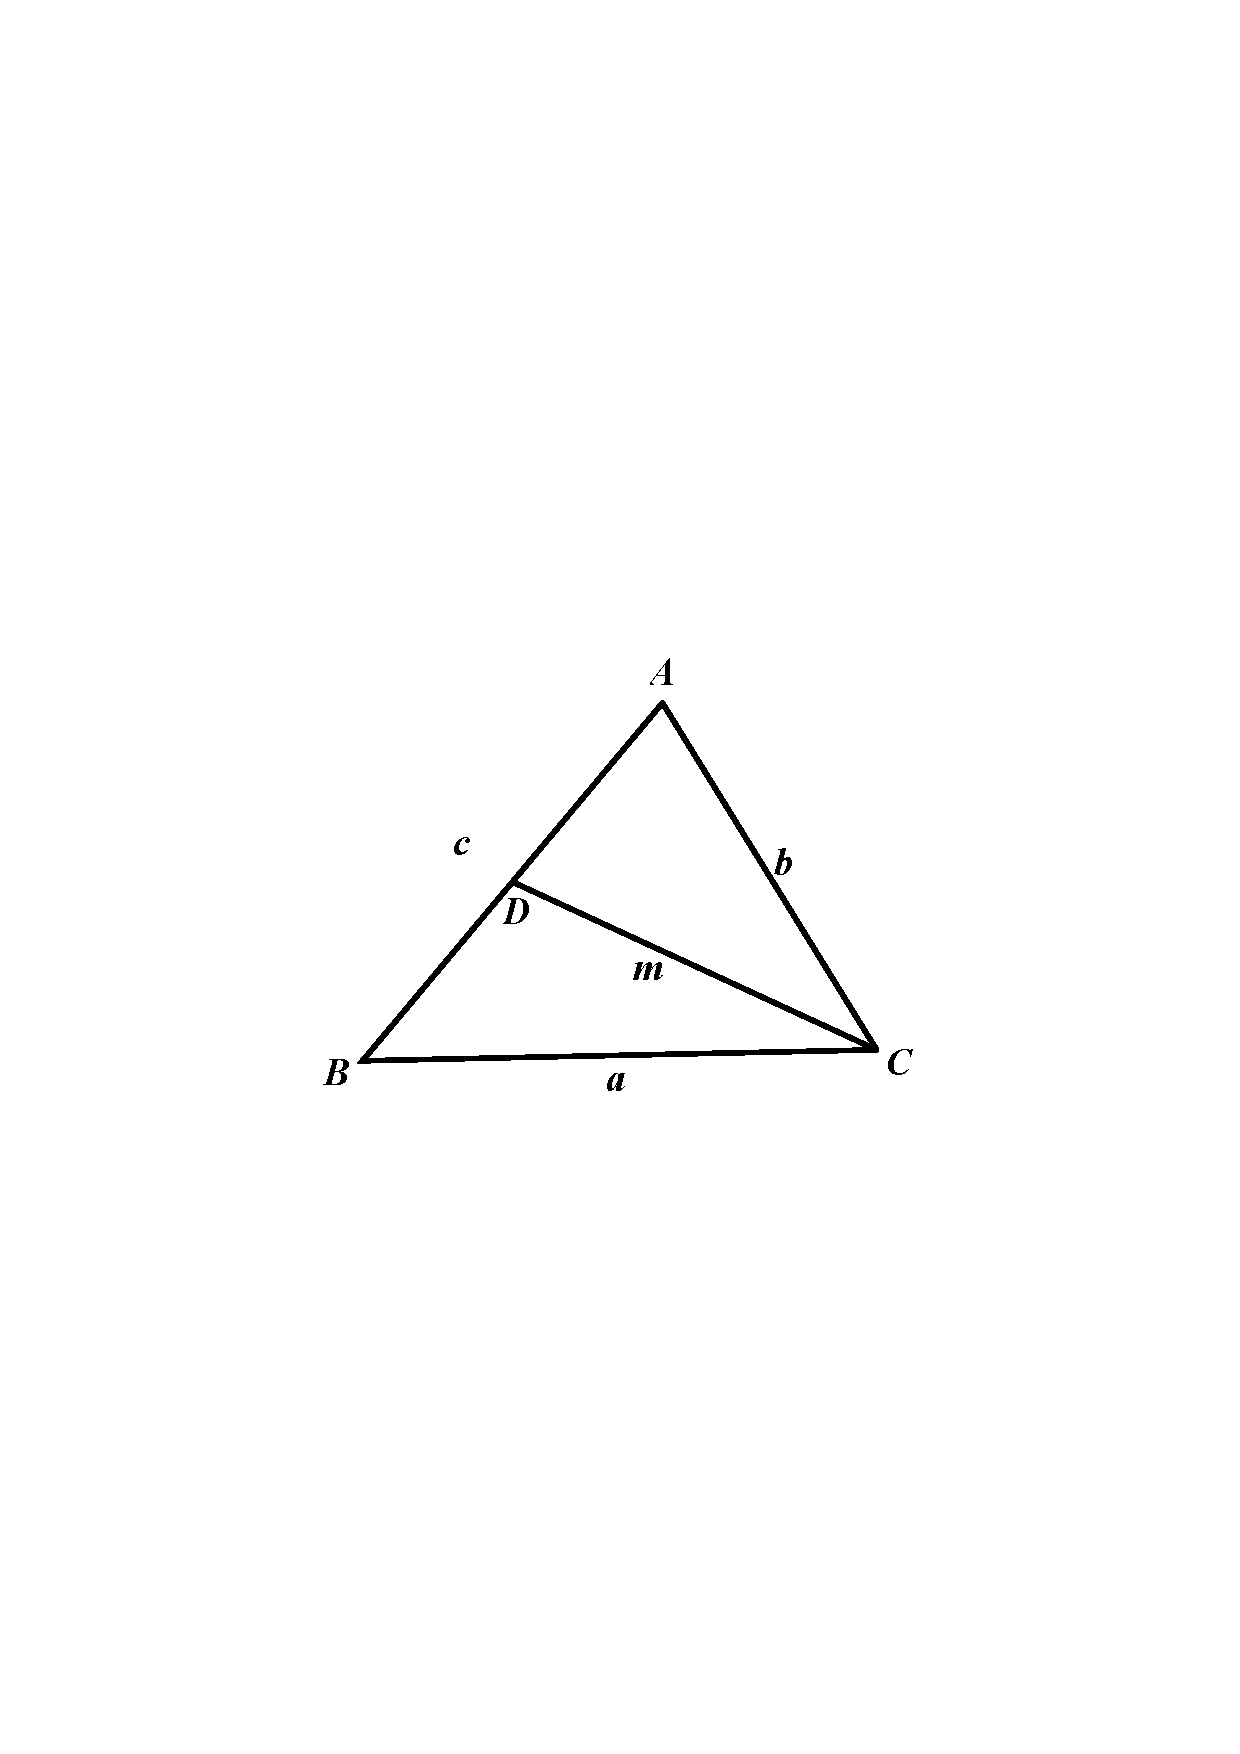
\includegraphics[width=0.4\linewidth]{PDF_Picture/三角形中线长公式}
\end{figure}

\item 对于任意四边形$ ABCD $,求证:$ \vec{AC}\perp
\vec{BD} $是$ BC^2+AD^2=BA^2+CD^2 $的充要条件。
\begin{figure}[H]
    \centering
    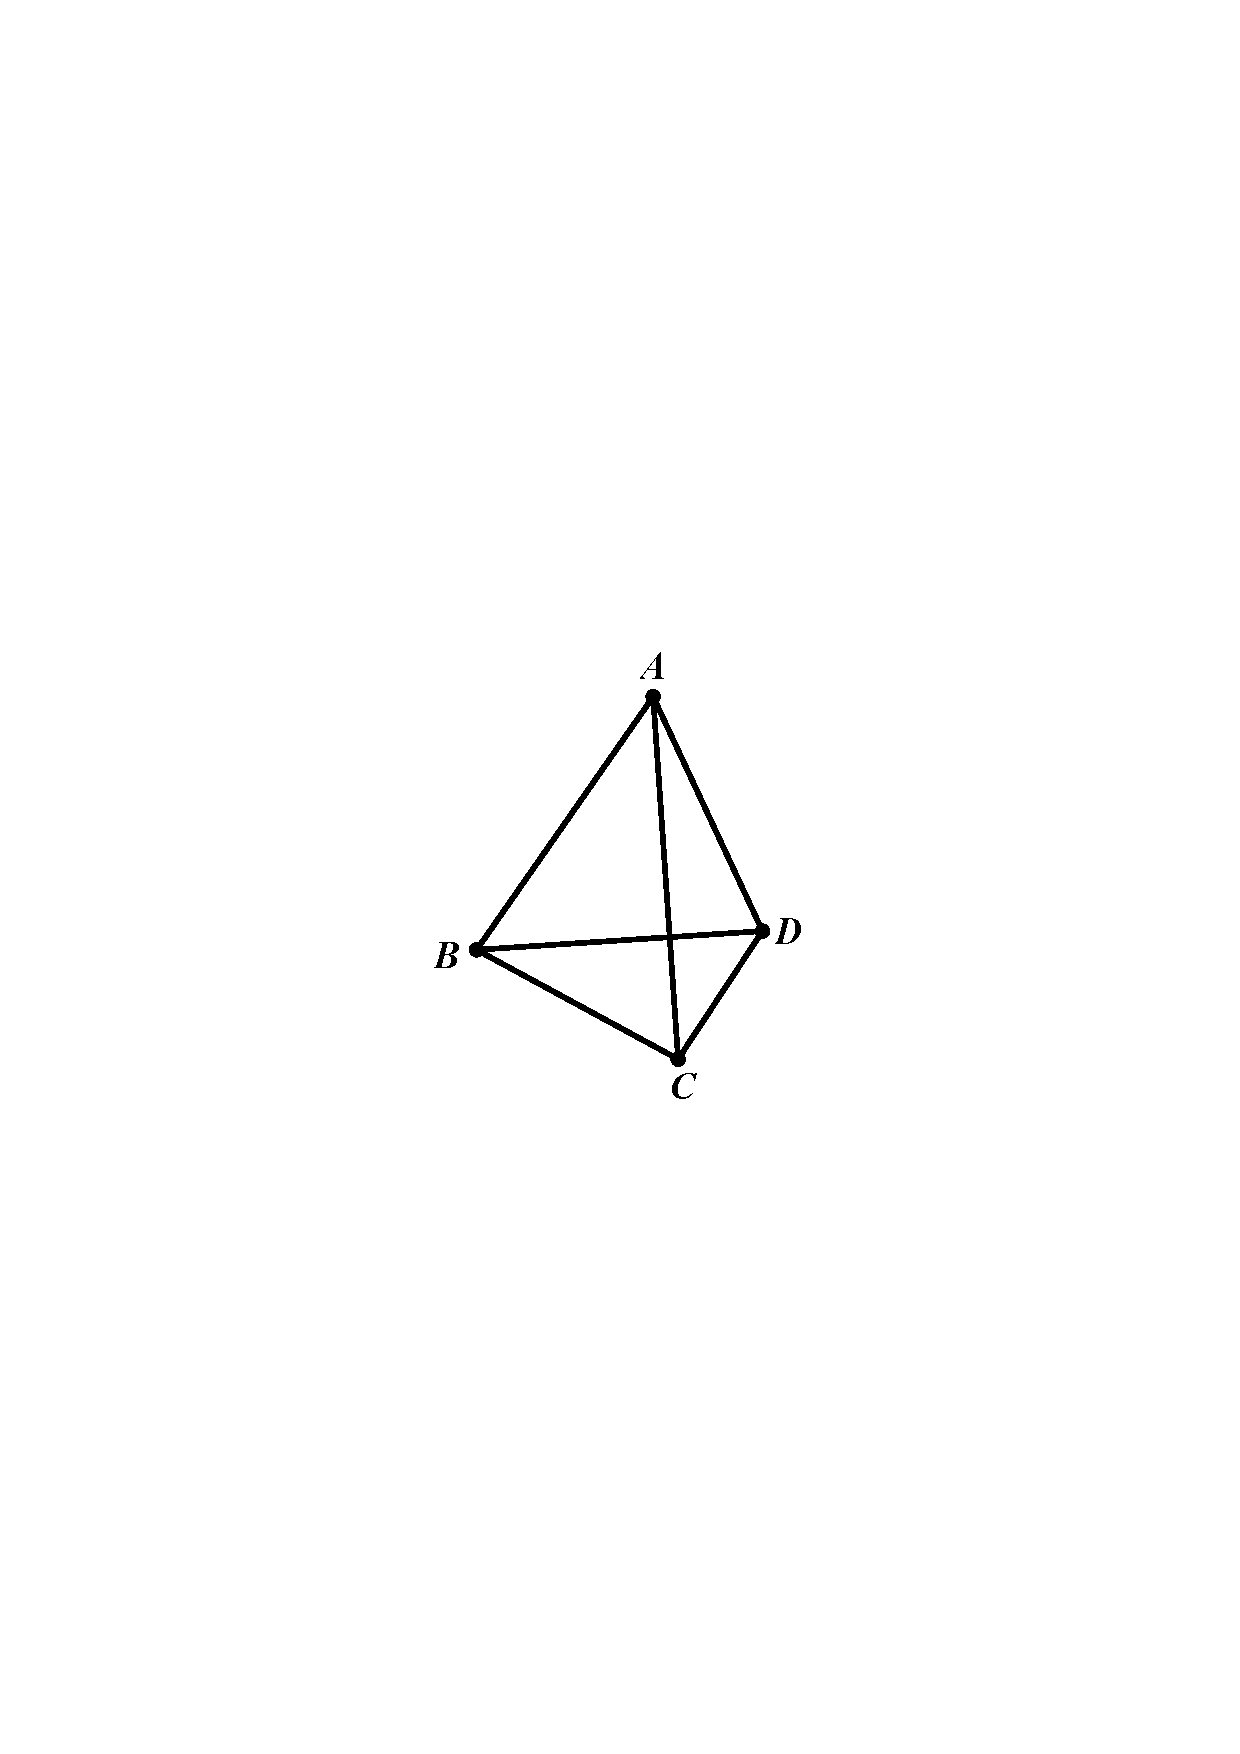
\includegraphics[width=0.26\linewidth]{对角线垂直的四边形}
    \caption{四边形$ ABCD $}
    \label{图8-1四边形ABCD}
\end{figure} 
\textbf{方法一}
\begin{align*}
    \vec{BC}\cdot\vec{BD}=\dfrac{BC^2+BD^2-CD^2}{2} \\
    \vec{BA}\cdot\vec{BD}=\dfrac{BA^2+BD^2-AD^2}{2} 
\end{align*}
两式相减:
\begin{align*}
    \vec{AC}\cdot\vec{BD}=\dfrac{BC^2+AD^2-BA^2-CD^2}{2}
\end{align*}
这说明$ \vec{AC}\perp \vec{BD} $是
$ BC^2+AD^2=BA^2+CD^2 $的充要条件。 \\
\textbf{方法二}\ 在空间中任取一点$ O $,由$ BC^2+AD^2=BA^2+CD^2 $可得:
\begin{gather*}
    (\vec{OC}-\vec{OB})^2 +
    (\vec{OD}-\vec{OA})^2 =
    (\vec{OA}-\vec{OB})^2 +
    (\vec{OD}-\vec{OC})^2  \quad \Leftrightarrow 	
\end{gather*}
\vspace{-0.8cm}
\begin{gather}\label{OAOBOCOD}
    \vec{OC}\cdot\vec{OB}+
    \vec{OD}\cdot\vec{OA}=
    \vec{OA}\cdot\vec{OB}+
    \vec{OD}\cdot\vec{OC} \quad \Leftrightarrow
\end{gather}
\vspace{-0.8cm}
\begin{gather*}	 
    (\vec{OC}-\vec{OA})
    \cdot(\vec{OB}-\vec{OD})=0 \quad \Leftrightarrow \\
    \vec{AC}\cdot\vec{DB}=0
\end{gather*}
(\ref{OAOBOCOD})式体现了$ A,B,C,D $四点的地位平等。

细心的读者应该能注意到,本题没有强调$ ABCD $是平面四边形还是空间四边形(三棱锥),
事实上对此没有要求,不论是哪种情形,以上两种证明过程都是成立的。

\item 现在我们把图\ref{图8-1四边形ABCD}看作是三棱锥,
假设其中两组对棱互相垂直,求证:第三组对棱也互相垂直。\\
\textbf{方法一}\ 设$ \vec{AB}\perp \vec{CD},\ 
\vec{AD}\perp \vec{BC} $,在空间中任取一点$ O $,那么
\begin{align*}
    (\vec{OA}-\vec{OB})\cdot
    (\vec{OC}-\vec{OD}) =&\ 0  \\
    (\vec{OA}-\vec{OD})\cdot
    (\vec{OB}-\vec{OC}) =&\ 0 
\end{align*}
由以上两式可得:
\begin{align}\label{三组对棱垂直的连等式}
    \vec{OA}\cdot \vec{OC}+
    \vec{OB}\cdot \vec{OD}=
    \vec{OA}\cdot \vec{OD}+
    \vec{OB}\cdot \vec{OC}=
    \vec{OA}\cdot \vec{OB}+
    \vec{OC}\cdot \vec{OD}
\end{align}
由(\ref{三组对棱垂直的连等式})式可得:$ \vec{AC}\cdot
\vec{DB}=0 $. (\ref{三组对棱垂直的连等式})式与(\ref{OAOBOCOD})式相似,
也与(\ref{垂心性质三个连等式})式相似。\\
\textbf{方法二}\ 设$ A $在平面$ BCD $上的投影的$ H $,
\begin{figure}[h]
    \centering
    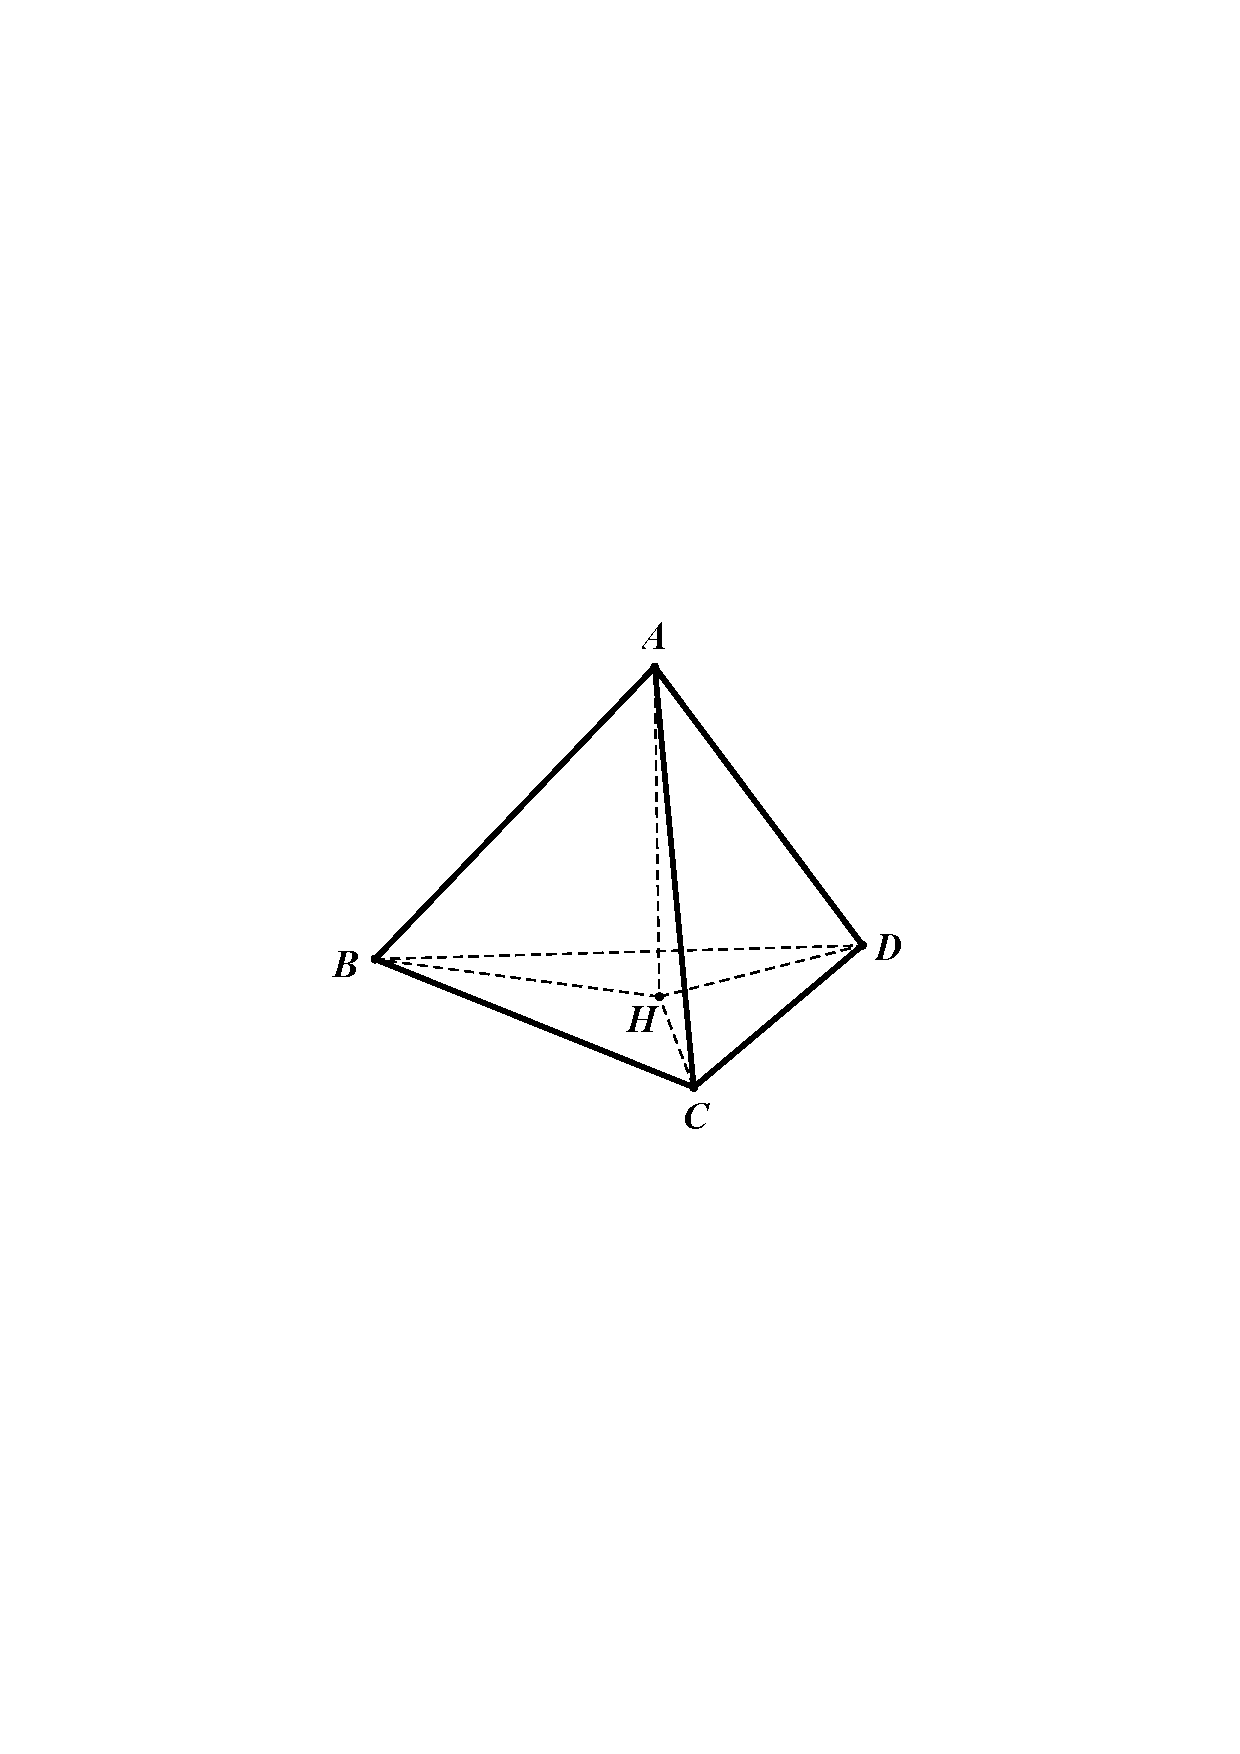
\includegraphics[width=0.25\linewidth]{三组对棱垂直}
\end{figure}
\begin{align*}
    AB\perp CD,\ AH\perp CD \Rightarrow BH\perp CD \\
    AD\perp BC,\ AH\perp BC \Rightarrow DH\perp BC 
\end{align*}
所以,$ H $为$ \Delta BCD $的垂心。$ CH\perp DB,\ AH\perp DB \Rightarrow 
AC\perp DB $. 

\item 考虑三角函数的万能代换,$ \sin\alpha=\dfrac{2\tan \frac{x}{2}}{1+\tan^2 \frac{x}{2}},\cos\alpha=\dfrac{1-\tan^2 \frac{x}{2}}{1+\tan^2 \frac{x}{2}} $,
如果令$ \tan\dfrac{x}{2}=\dfrac{b}{a} $,那么
\begin{align*}
    \sin\alpha=\dfrac{\frac{2b}{a}}{1+\left(\frac{b}{a}\right)^2}=
    \dfrac{2ab}{a^2+b^2},\quad\quad \cos\alpha=\dfrac{1-\left(\frac{b}{a}
    \right)^2}{1+\left(\frac{b}{a}\right)^2}=\dfrac{a^2-b^2}{a^2+b^2}
\end{align*}
利用$ \cos^2 \alpha+\sin^2 \alpha=1 $,可得到
\begin{gather}\label{勾股定理正整数解通式}
    (a^2-b^2)^2+(2ab)^2=(a^2+b^2)^2
\end{gather}
令$ x=a^2-b^2,\ y=2ab,\ z=a^2+b^2 $,那么上式变成$ x^2+y^2=z^2 $,
具有勾股定理的形式。$ a^2-b^2 $和$ 2ab $分别是$ (a+b\i)^2=(a^2-b^2)+2ab\i $
的实部和虚部。
让$ a,b (a\neq b) $取正整数,就能得到勾股数,所以,方程$ x^2+y^2=z^2 $
有无穷多组整数解\footnote{费马大定理:当整数
$ n\geq 3 $时,方程$ x^n+y^n=z^n $没有$ xyz\neq 0 $的整数解(也可等价地表述为
没有正整数解)。
感兴趣的读者可以探讨:方程$ k_1 x^n+k_2 y^n=k_3 z^n \ 
(k_1,k_2,k_3\in \textbf{Z},\ n\geq 2 ) $ 是否有正整数解。}。
对于该方程的整数解,$ x,y $不可能同时是奇数。
常见的勾股数有 $ (3,4,5)$, $(5,12,13)$, $(7,24,25)$, 
$(8,15,17)$, $(9,40,41)$, $(11,60,61)$, $(20,21,29) $. 
可以证明:任意一组勾股数的乘积都是60的倍数\footnote{
参见 https://www.zhihu.com/question/1896886358745805689}。

若把(\ref{勾股定理正整数解通式})式中的$ a^2,b^2 $换成$ a,b $,有
\begin{align*}
    (a-b)^2+4ab=(a+b)^2
\end{align*}
再把上式的$ a,b $换成向量$ \vec{a},\vec{b} $,然后移项,有
\begin{align}\label{极化恒等式}
    4 \vec{a}\cdot \vec{b}=
    (\vec{a}+\vec{b})^2-(\vec{a}-\vec{b})^2
\end{align}
(\ref{极化恒等式})式被称为极化恒等式。

\item 海伦公式。设$ \Delta ABC $的三条边长分别为$ a,b,c $,
令$ p=\dfrac{a+b+c}{2} $,为三角形周长的一半,
则$ S_{\Delta ABC}=\sqrt{p(p-a)(p-b)(p-c)} $. \ 证明如下:
\begin{align*}
    S_{\Delta ABC}^2=&\ \left(\dfrac{1}{2}ab\sin C \right) ^2=
    \dfrac{1}{4}a^2b^2\left[ 1-\left( {\dfrac{a^2+b^2-c^2}{2ab}}\right)^2 \right] 
\end{align*}
将括号展开后可得:
\begin{align*}
    S_{\Delta ABC}^2=\dfrac{1}{16}\left[-(a^4+b^4+c^4)+2(a^2b^2+b^2c^2+c^2a^2)\right]
\end{align*}
不做展开,而进行因式分解可得:
\begin{align*}
    S_{\Delta ABC}^2
    =&\ \left[ \dfrac{1}{2}ab+\dfrac{1}{4}
    (a^2+b^2-c^2)\right] \left[ \dfrac{1}{2}ab-\dfrac{1}{4} (a^2+b^2-c^2) \right] \\
    =&\ \left[  \dfrac{1}{4}(a+b)^2-\dfrac{1}{4}c^2 \right] 
    \left[ -\dfrac{1}{4}(a-b)^2+\dfrac{1}{4}c^2 \right] \\
    =&\ \left(\dfrac{a+b+c}{2}\right) \left(\dfrac{a+b-c}{2}\right) 
    \left(\dfrac{b+c-a}{2}\right) \left(\dfrac{a+c-b}{2}\right) \\
    =&\ p(p-a)(p-b)(p-c)
\end{align*}
若$ p $是定值(即三角形的周长固定),根据均值不等式,有
\begin{gather}\label{正三角形面积最大}
    p(p-a)(p-b)(p-c)\leq p\left[\dfrac{(p-a)+(p-b)+(p-c)}{3}\right]^3=\dfrac{p^4}{27}
\end{gather}
以上的等号在$ a=b=c $时成立,所以,在周长固定的情况下,等边三角形的面积最大。

记$ u=a^4+b^4+c^4,\ v=a^2b^2+b^2c^2+c^2a^2 ,\ w=a^2+b^2+c^2 $,
那么$ w^2=u+2v $,根据柯西不等式:$ u\geq v $,那么$ w^2=u+2v \geq 3(-u+2v)=
48 \cdot \dfrac{-u+2v}{16}=48 S_{\Delta ABC}^2 $,开平方后有:
$ w\geq 4\sqrt{3}S_{\Delta ABC} $,即
\begin{gather}\label{外森比克不等式}
    a^2+b^2+c^2 \geq 4\sqrt{3}S_{\Delta ABC}
\end{gather}
此不等式被称为外森比克(Weitzenböck)不等式。
等号成立的条件是$ a=b=c $,即$ \Delta ABC $
是等边三角形。再利用余弦定理来逆向分析外森比克不等式,
$ a^2+b^2+c^2=a^2+b^2+(a^2+b^2-2ab\cos C)\geq 4\sqrt{3}\cdot
\dfrac{1}{2}ab\sin C $,移项,
$ 2(a^2+b^2)\geq 2ab(\cos C+\sqrt{3}\sin C)=4ab\sin(C+\dfrac{\pi}{6}) $,
此不等式显然成立。 所以,当$ a^2+b^2+c^2=4\sqrt{3}S_{\Delta ABC}=
\begin{cases}
    2\sqrt{3}ab\sin C \\
    2\sqrt{3}bc\sin A \\
    2\sqrt{3}ac\sin B
\end{cases}$时,$ \Delta ABC $一定是等边三角形。

\item 三角形面积公式汇总:
\begin{gather}\label{三角形面积公式汇总}
    \left.    
    \begin{gathered}
        S=\dfrac{1}{2}ab\sin C=\dfrac{1}{2}bc\sin A=\dfrac{1}{2}ac\sin B=\\ 
        2R^2\sin A\sin B\sin C=\dfrac{abc}{4R}=\sqrt{p(p-a)(p-b)(p-c)}=pr
    \end{gathered} \right\}
\end{gather}
其中,$ R $是外接圆半径,$ r $是内切圆半径,$ p $为半周长。

\item 外森比克不等式的等价形式:
\begin{align*}
    a^2+b^2+c^2 &=2bc\cos A+2ac\cos B+2ab\cos C \\
    &=8R^2(\sin B\sin C\cos A+\sin A\sin C\cos B+\sin A\sin B\cos C) \\
    &\geq 4\sqrt{3}S_{\Delta}=4\cdot 2R^2\sin A\sin B\sin C
\end{align*}
两边约去$ 8R^2 $后可得:
\begin{gather*}
    \sin B\sin C\cos A+\sin A\sin C\cos B+\sin A\sin B\cos C
    \geq \sqrt{3} \sin A\sin B\sin C
\end{gather*}

\item $^*$ 设三角形的三条边长分别为$ a,b,c $,请思考:\\
\ding{192} 给定约束条件$ \lambda_1 a+\lambda_2 b+\lambda_3 c=\mu $,
($ \lambda_1,\lambda_2,\lambda_3,\mu $均为正数),三角形的面积何时最大?\\
\ding{193} 给定约束条件$ \lambda_1 a^2+\lambda_2 b^2+\lambda_3 c^2=\mu $,
($ \lambda_1,\lambda_2,\lambda_3,\mu $均为正数),三角形的面积何时最大?\\
对于\ding{192},容易想到
\begin{align*}
    p(p-a)(p-b)(p-c)=&\ \dfrac{p}{\lambda_1 \lambda_2 \lambda_3}
    (\lambda_1 p-\lambda_1 a)(\lambda_2 p-\lambda_2 b)
    (\lambda_3 p-\lambda_3 c)\\ \leq&\ 
    \left[\dfrac{\left(\frac{1}{\lambda_1
            \lambda_2 \lambda_3}+\lambda_1+\lambda_2+
        \lambda_3\right)p-\mu}{4}\right]^4
\end{align*}
但是,$ p=\dfrac{1}{2}(a+b+c) $不再是常数,而且等号很可能无法成立,
所以上面方法不可行。\\
对于\ding{193},利用
\begin{gather*}
    S=\frac{1}{2}ab\sin C=\frac{1}{2}\sqrt{a^2b^2(1-\cos^2 C)}=
    \frac{1}{2}\sqrt{a^2b^2-\frac{1}{4}(a^2+b^2-c^2)^2}  \\
    = \frac{1}{2}\sqrt{a^2b^2-\frac{1}{4}\left(a^2+b^2-
        \dfrac{\mu-\lambda_1 a^2-\lambda_2b^2}{\lambda_3}\right)^2}
\end{gather*}
令$ M=\dfrac{1}{\left(1+\frac{\lambda_1}{\lambda_3}\right)
    \left(1+\frac{\lambda_2}{\lambda_3}\right)} $,
$ u=\left(1+\dfrac{\lambda_1}{\lambda_3}\right)a^2 $,
$ v=\left(1+\dfrac{\lambda_2}{\lambda_3}\right)b^2 $,则
\begin{gather*}
    a^2b^2=Muv \leq M\left(\dfrac{u+v}{2}\right)^2 \\
    S\leq \frac{1}{2}\sqrt{M\left(\dfrac{u+v}{2}\right)^2
        -\frac{1}{4}\left(u+v-\mu \right)^2} 
\end{gather*}
再做变量代换$ t=u+v $,根号下就是关于$ t $的二次函数,剩余略。

\item $ \Delta ABC $的$ BC $边上有$ n $个点,记为$ P_1,P_2,\cdots P_n $,
设$ \vec{AP_1}+\vec{AP_2}+\cdots +\vec{AP_n}=
\lambda \vec{AB} +\mu \vec{AC} $,则$ \lambda+\mu=n $. \begin{figure}[h]
    \centering
    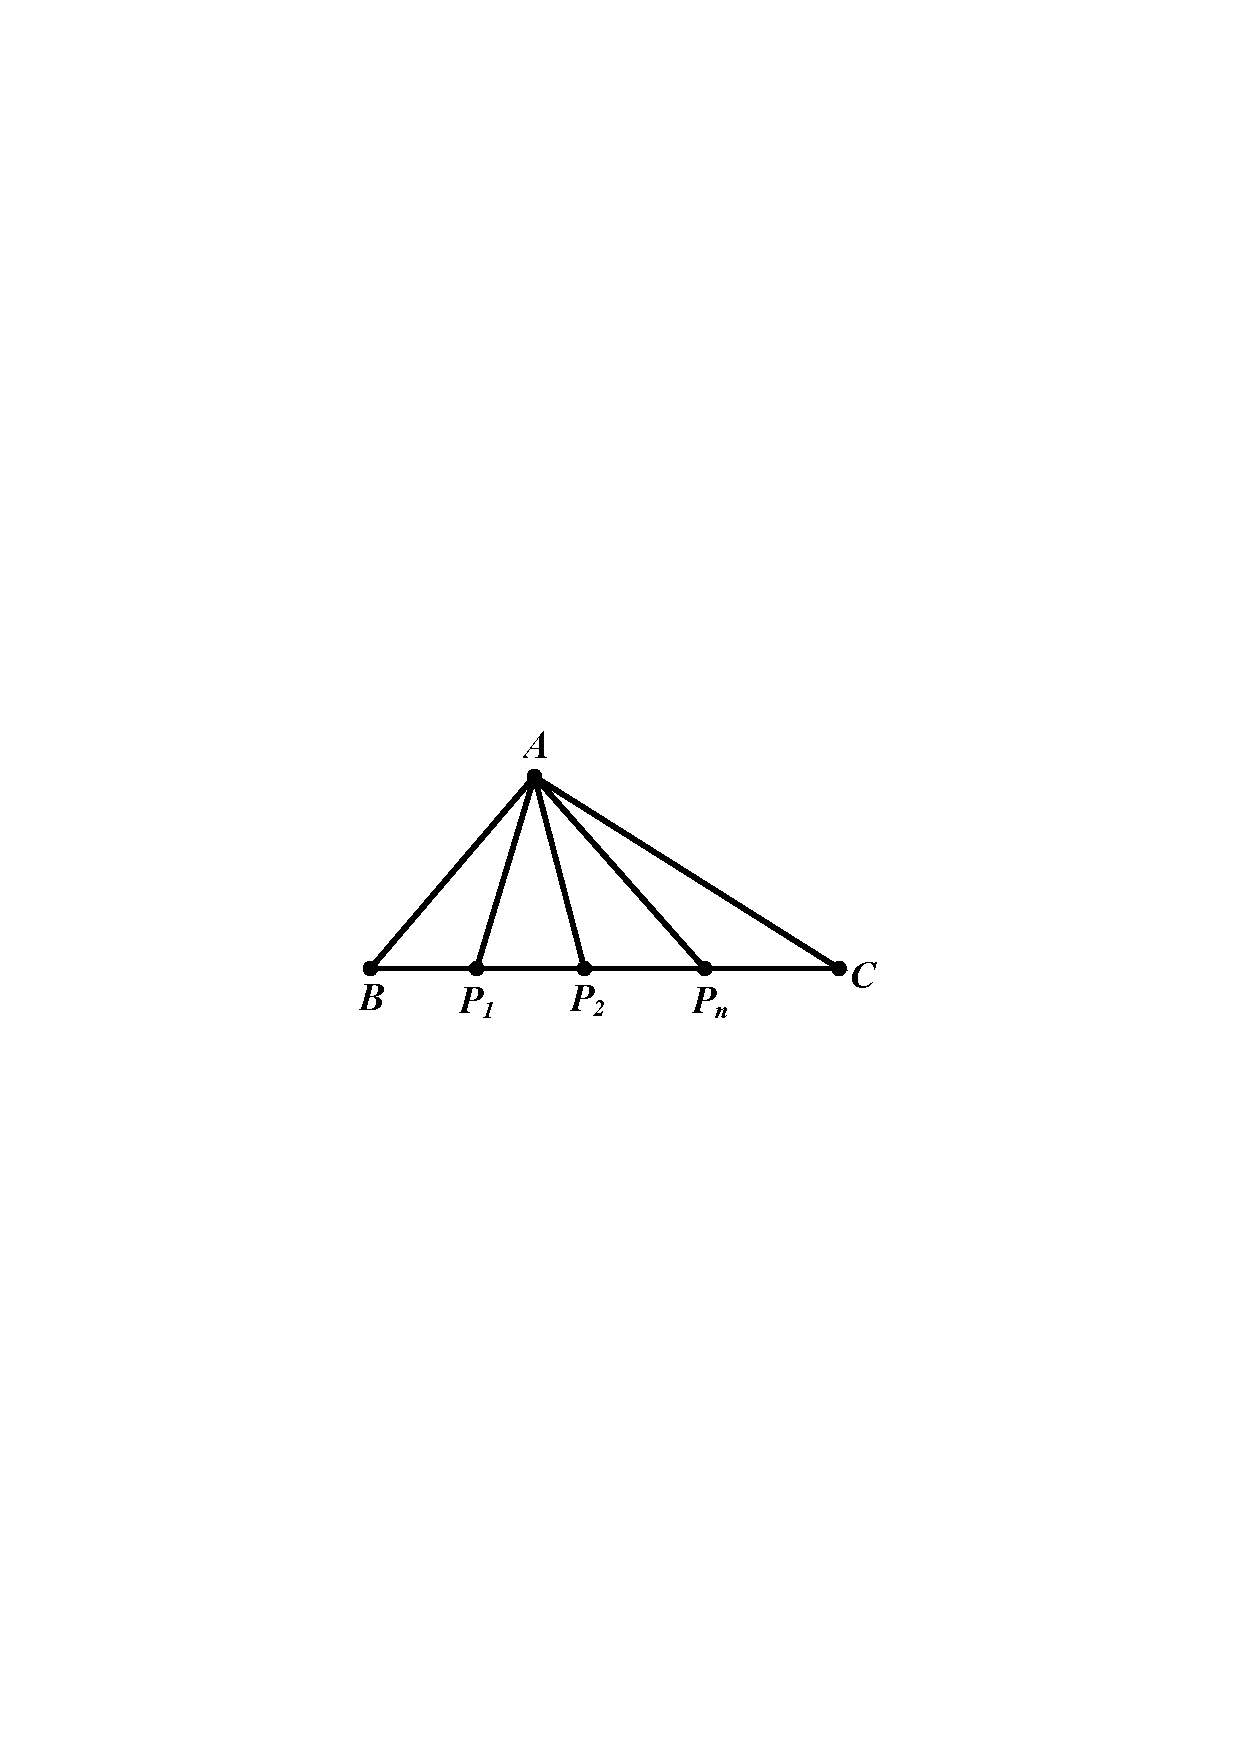
\includegraphics[width=0.3\linewidth]{多个向量终点共线}
\end{figure}

\end{itemize}

\section{重心、垂心、内心、外心}
\begin{itemize}[leftmargin=\inteval{\myitemleftmargin}pt,itemsep=
   \inteval{\myitemitempsep}pt,topsep=\inteval{\myitemtopsep}pt]
\item $ \Delta ABC $的三条中线交于一点$ G $(重心),三条中线
把三角形分成6个面积相等的小三角形。重心分割中线的比例为1:2,证明如下:
\begin{figure}[h]
    \centering
    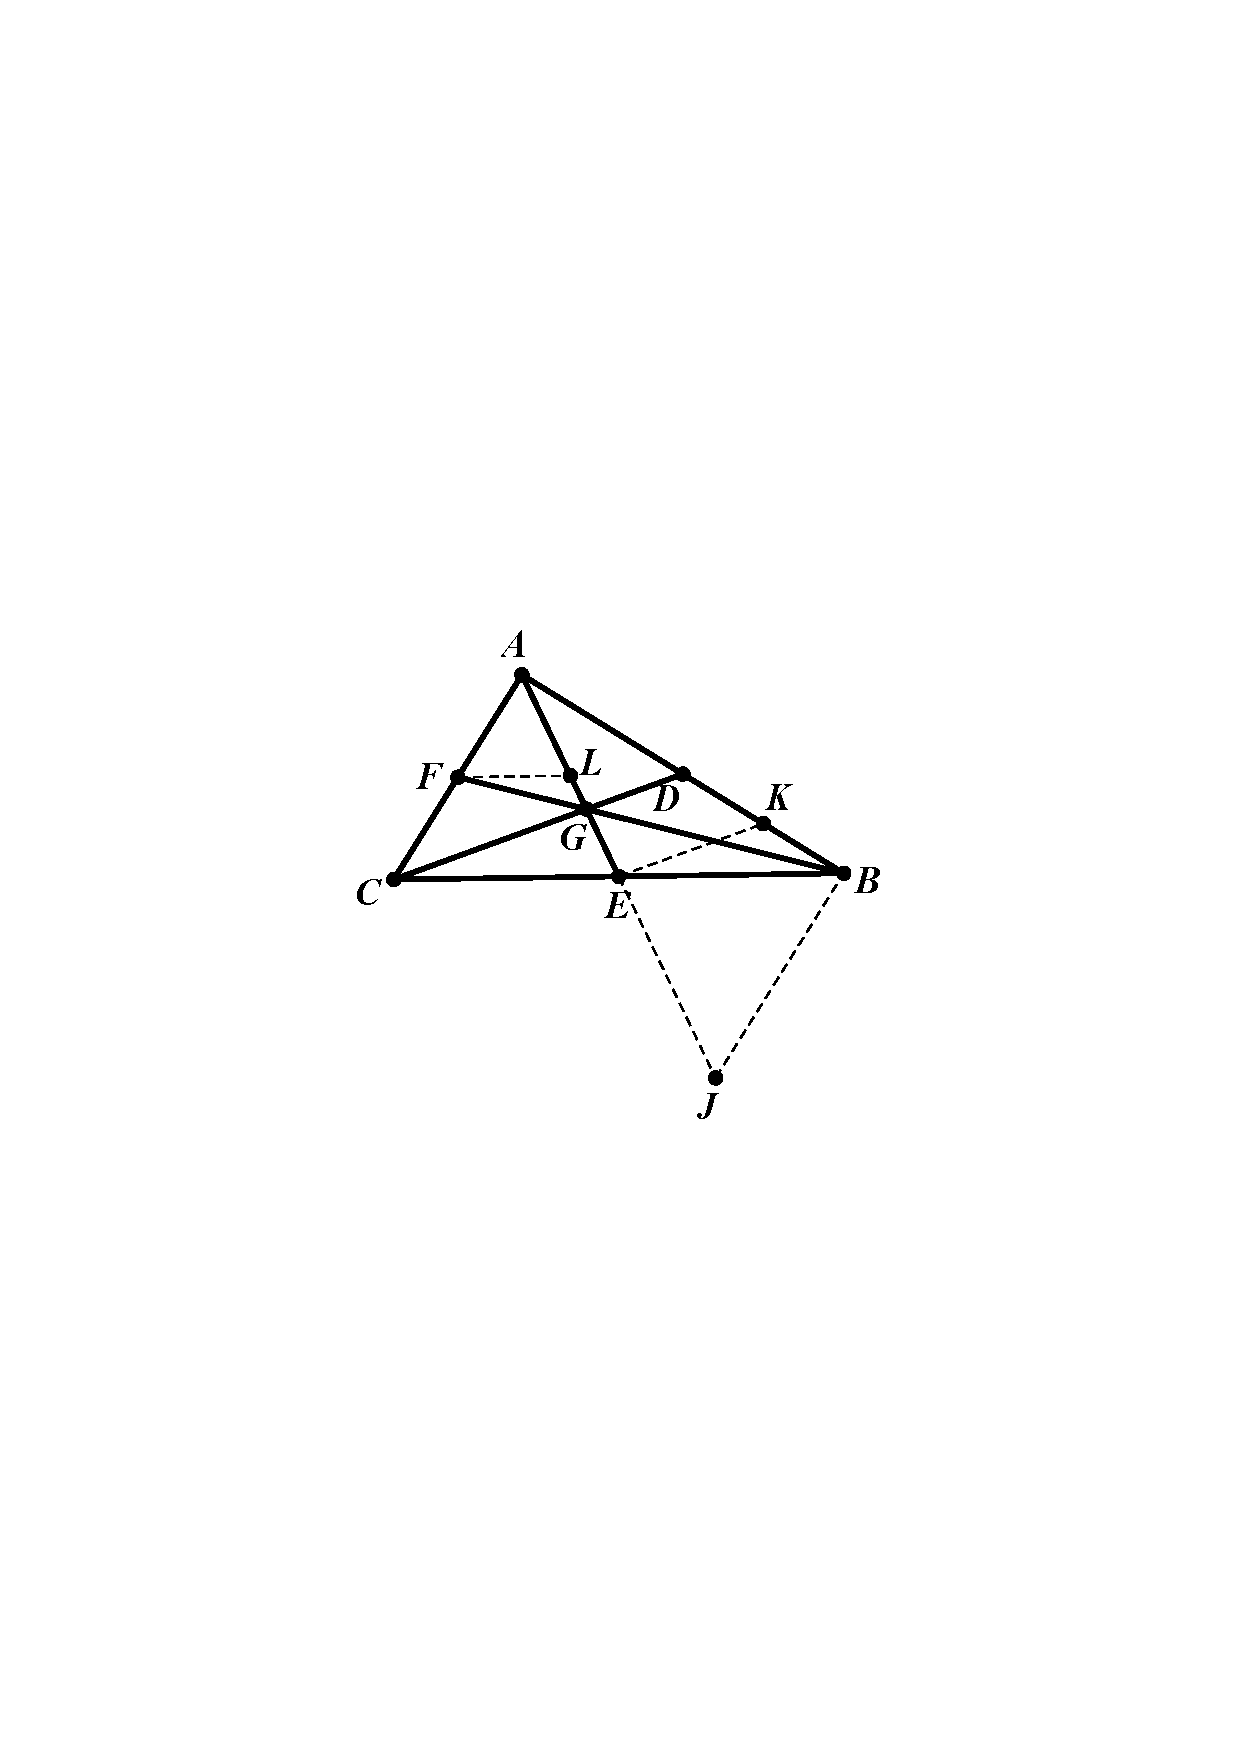
\includegraphics[width=0.3\linewidth]{重心性质证明}
\end{figure} \\
\textbf{方法一}\ 过$ B $点做$ AC $的平行线,与$ AE $的延长线交于点$ J $,容易看出
$ \Delta AFG \backsim \Delta JBG $(因为三组对应角相等),所以$ \dfrac{BG}{FG}=
\dfrac{JB}{AF}=2 $. \\
\textbf{方法二}\ 过$ E $点做$ CD $的平行线,与$ AB $交于点$ K $,容易看出
$ \Delta BEK \backsim \Delta BCD,\\ \Delta AGD \backsim \Delta AEK $,所以
$ DK=BK=\dfrac{1}{2}AD,\ \dfrac{AG}{GE}=\dfrac{AD}{DK}=2 $. \\
\textbf{方法三}\ 过$ F $点做$ CB $的平行线,与$ AE $交于点$ L $,容易看出
$ \Delta LFG \backsim \Delta EBG $,所以$\dfrac{BG}{FG}=\dfrac{BE}{FL}=2 $. \\
\textbf{方法四}\ 向量法,在$ \Delta ABC $中,$ AB $边的中点为$ D $,
$ BC $边的中点为$ E $,$ CA $边的中点为$ F $. 
\begin{align*}
    & \vec{AG}=\lambda \vec{AD}+(1-\lambda)\vec{AC}=
    \mu \vec{AF}+(1-\mu)\vec{AB} \\
    & \vec{AG}=\dfrac{\lambda}{2} \vec{AB}+(1-\lambda)\vec{AC}=
    \dfrac{\mu}{2} \vec{AC}+(1-\mu)\vec{AB} 
\end{align*}
则 $ \begin{cases}
    \dfrac{\lambda}{2} =\ 1-\mu  \\
    \dfrac{\mu}{2} =\ 1-\lambda
\end{cases} $,解得$ \lambda=\mu=\dfrac{2}{3} $,即$ \vec{AG}=
\dfrac{2}{3}\vec{AD}+\dfrac{1}{3}\vec{AC}=
\dfrac{2}{3}\vec{AF}+\dfrac{1}{3}\vec{AB} $,
已经能说明重心分割中线的比例为1:2. 所以$ \vec{AG}=
2\vec{GE}=\vec{GB}+\vec{GC}, 
\ \vec{GA}+\vec{GB}+\vec{GC}=
\vec{0} $. 再设$ O $为空间中的任意一点,则
\begin{align*}
    \vec{OG}=\vec{OA}+\vec{AG} =&\ 
    \vec{OA}+\dfrac{1}{3}\left(\vec{AB}+
    \vec{AC} \right) \\
    =&\ \vec{OA}+\dfrac{1}{3} \left[\left( \vec{OB} 
    -\vec{OA}\right) + \left( \vec{OC} -\vec{OA}\right)\right]  \\
    =&\ \dfrac{1}{3}\left(\vec{OA}+\vec{OB}+
    \vec{OC} \right) 
\end{align*}

\item 四面体的重心是4个顶点与对面重心连线的交点,重心分连线的比例为3:1,
重心也是与四个顶点连线长度的平方和最小的点。

\item 在$ \Delta ABC $中,$ D $是$ BC $边上一点,且$ \vec{BD}=\mu_1
\vec{BC},\ 0<\mu_1<1 $. $ E $是$ AD $上一点,$ \vec{AE} =
\mu_2\vec{AD},\ 0<\mu_2<1 $. 过$ E $点的直线与$ AB,AC $所在的直线分别交于
$ M,N $两点,设$ \vec{AM}=x\vec{AB},\vec{AN}=
y\vec{AC} $,求证:
$ \dfrac{(1-\mu_1)\mu_2}{x}+\dfrac{\mu_1\mu_2}{y}=1 $. 
\begin{figure}[h]
    \centering
    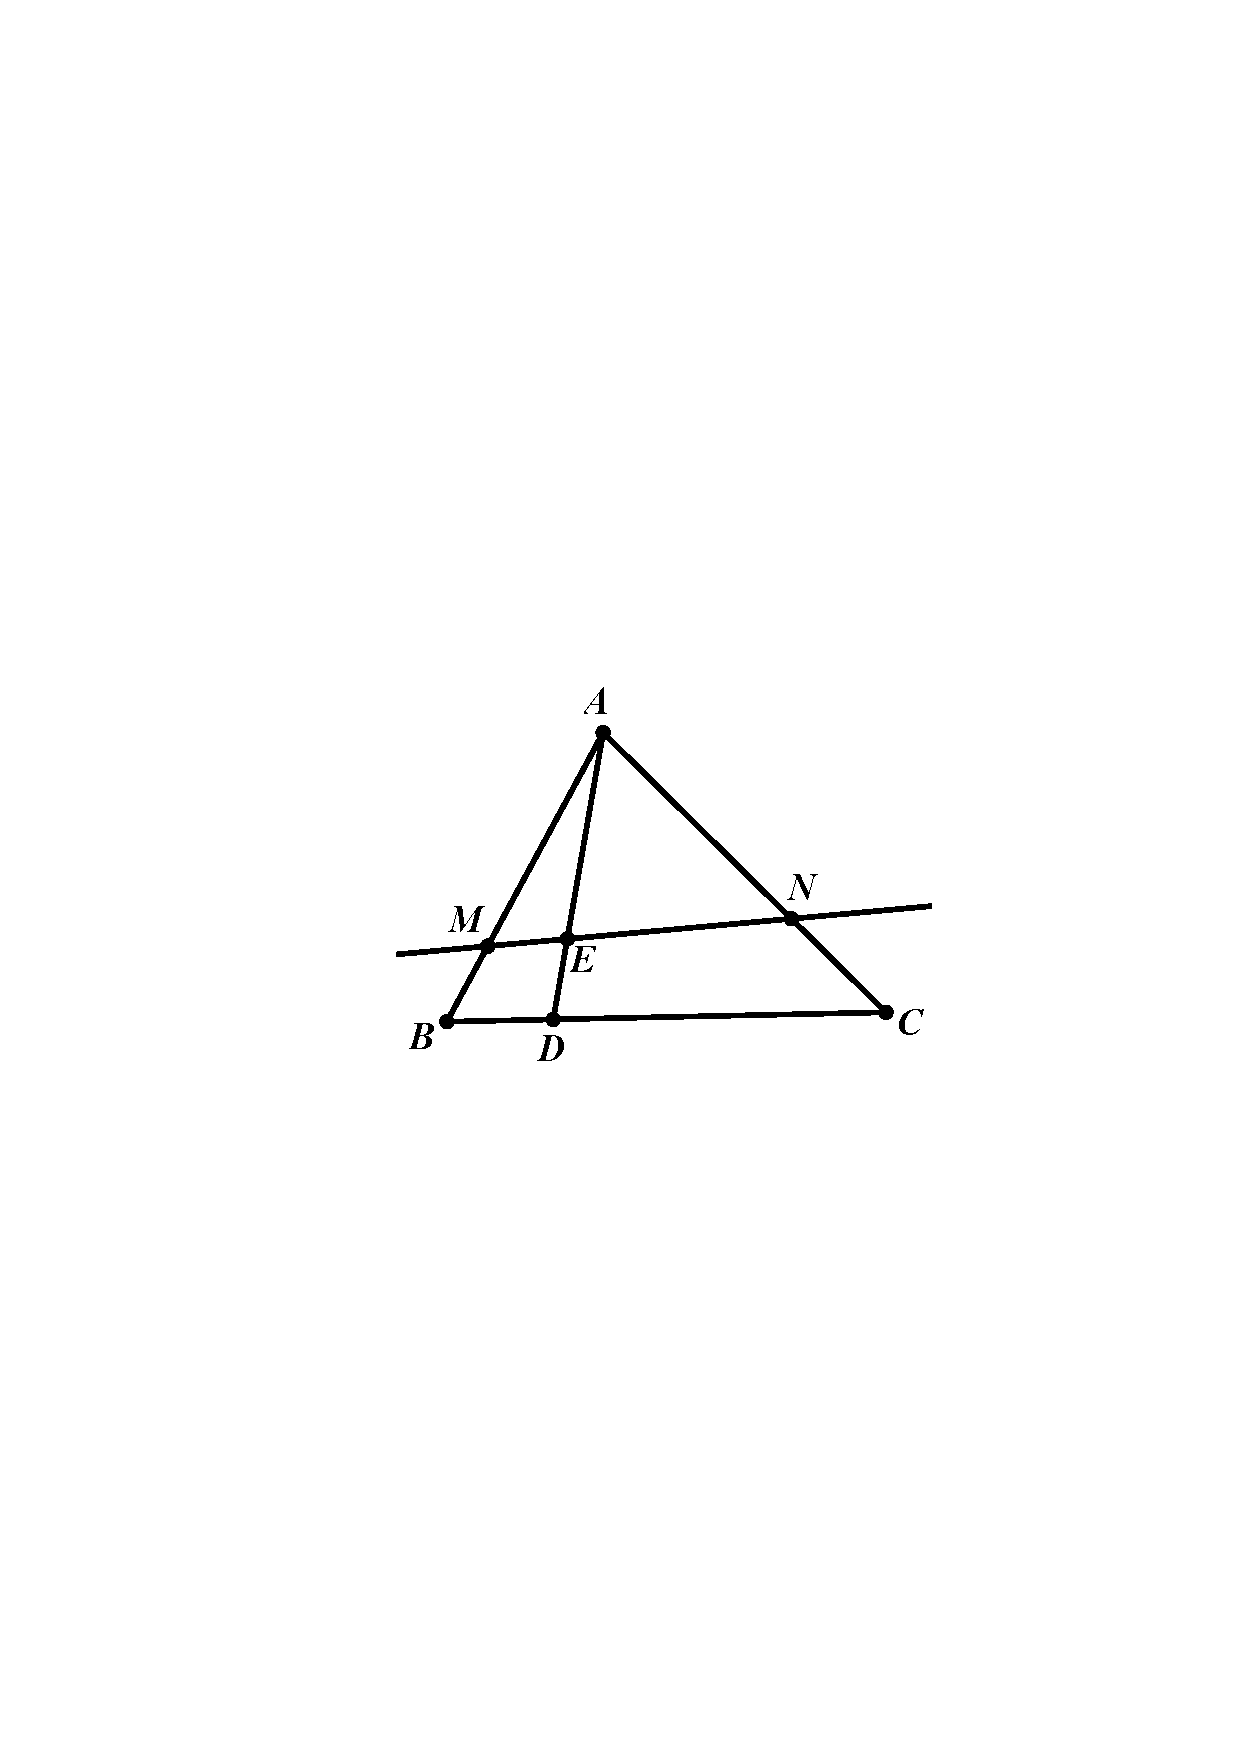
\includegraphics[width=0.3\linewidth]{系数倒数相加为定值}
\end{figure} \\
\textbf{方法一}\ 向量法
\begin{align*}
    \vec{AE} =\mu_2\vec{AD} =&\ \mu_2\left[
    (1-\mu_1)\vec{AB}+\mu_1\vec{AC}\right]\\
    =&\ (1-\mu_1)\mu_2\vec{AB}+\mu_1\mu_2\vec{AC} \\
    \vec{AE}=\lambda\vec{AM}+(1-\lambda)
    \vec{AN}=&\ \lambda x\vec{AB}+(1-\lambda)y
    \vec{AC}
\end{align*}
$ \begin{cases}
    \lambda x = (1-\mu_1)\mu_2 \\
    (1-\lambda)y = \mu_1\mu_2
\end{cases} $. 所以$ \dfrac{(1-\mu_1)\mu_2}{x}+\dfrac{\mu_1\mu_2}{y}
=\lambda+1-\lambda=1 $. \\
当$ E $是三角形的重心时,$ \mu_1=\dfrac{1}{2},\ \mu_2=\dfrac{2}{3},\ 
\dfrac{1}{x}+\dfrac{1}{y}=3 $. \\
\textbf{方法二}\ 面积法。
\begin{gather*}
    \dfrac{S_{\Delta AME}+S_{\Delta ANE}}{S_{\Delta ABC}}=
    \dfrac{S_{\Delta AMN}}{S_{\Delta ABC}}=\dfrac{|AM|\cdot 
    |AN|\cdot\sin\angle BAC}
    {|AB|\cdot |AC|\cdot\sin\angle BAC}=xy \\
    \dfrac{S_{\Delta AME}}{S_{\Delta ABC}}=\dfrac{S_{\Delta AME}}
    {S_{\Delta ABD}}\cdot \dfrac{S_{\Delta ABD}}{S_{\Delta ABC}}=x\mu_2\cdot\mu_1 \\
    \dfrac{S_{\Delta ANE}}{S_{\Delta ABC}}=y\mu_2\cdot(1-\mu_1)
\end{gather*}
于是有$ x\mu_2\mu_1+y\mu_2(1-\mu_1)=xy $,两边同除$ xy $即得结论。

\item 设$ \Delta ABC $的垂心为$ H $,则$ \vec{HA}\cdot \vec{BC}=
\vec{HA}\cdot (\vec{HC}-\vec{HB})=
\vec{0},\ \vec{HA}\cdot \vec{HC}=
\vec{HA}\cdot \vec{HB} $,采用类似方法,可以得到
\begin{align}\label{垂心性质三个连等式}
    \vec{HA}\cdot \vec{HB}=
    \vec{HA}\cdot \vec{HC}=\vec{HB}\cdot \vec{HC} 
\end{align}
\begin{figure}[h]
    \centering
    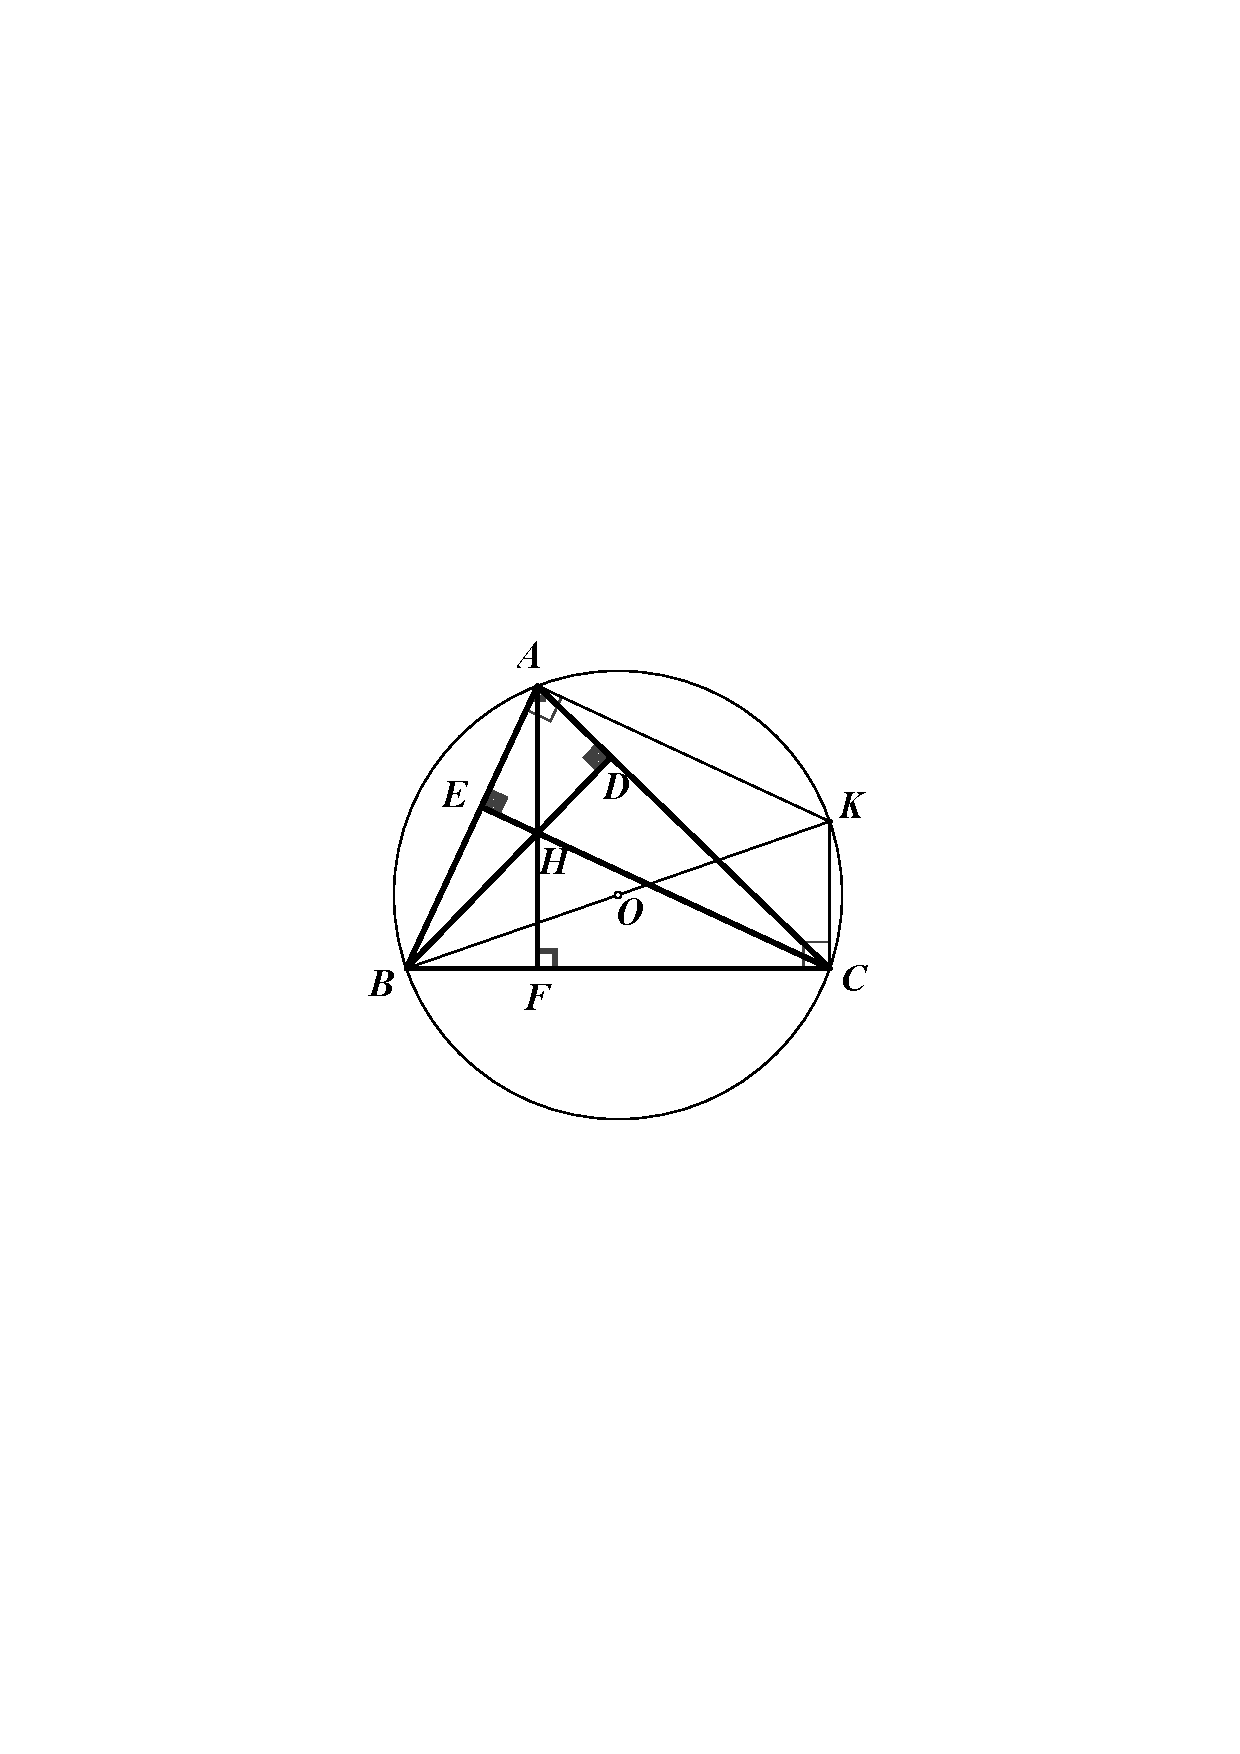
\includegraphics[width=0.3\linewidth]{垂心的性质}
\end{figure}
考虑$ \Delta AHB,\Delta BHC,\Delta CHA $的面积比,
\begin{gather*}
    \dfrac{S_{\Delta AHB}}{S_{\Delta BHC}}=\dfrac{HB\cdot AD}
    {HB \cdot CD}=\dfrac{AD}{CD}=\dfrac{\dfrac{BD}{\tan A}}
    {\dfrac{BD}{\tan C}}=\dfrac{\tan C}{\tan A} \\
    S_{\Delta BHC}:S_{\Delta CHA}:S_{\Delta AHB}= \tan A:\tan B:\tan C
\end{gather*}
四边形$ AEHD $有两个内角为直角,所以$ \angle EAD+\angle EHD=\angle EAD
+\angle BHC =\pi $,同理可得:
$ \angle BCA+\angle BHA =\pi,\ \angle ABC+\angle AHC =\pi $. 

\item 设$ \Delta ABC $的内心为$ I $,若$ \vec{AI}=\lambda\vec{AB}+\mu\vec{AC} $,
则$ \lambda:\mu=|\vec{AC}|:|\vec{AB}| $. 
\begin{figure}[h]
    \centering
    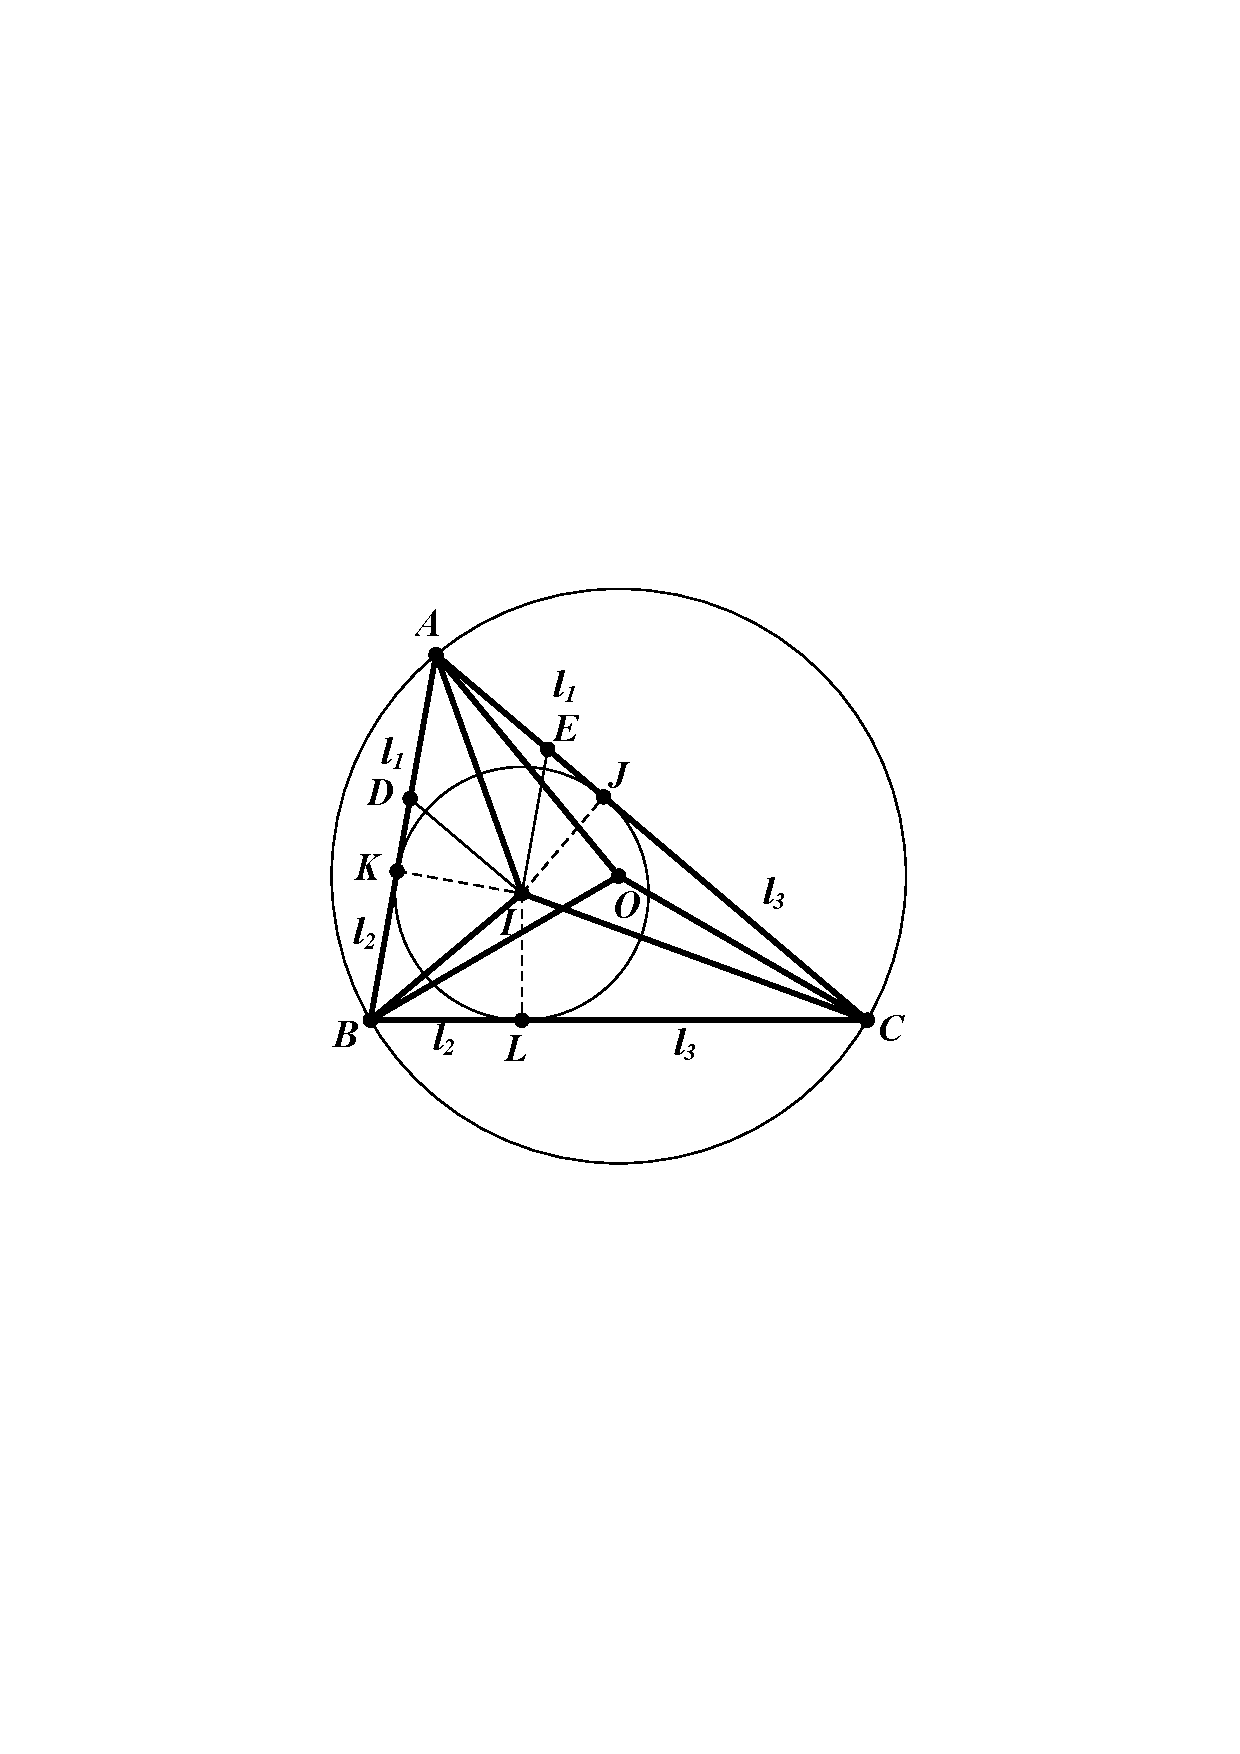
\includegraphics[width=0.4\linewidth]{内心外心合并图}
\end{figure}
\\
\textbf{证}\ 过$ I $点作$ AB,AC $的平行线,与$ AB,AC $分别交于$ D,E $两点,
则$ \vec{AD}=\lambda\vec{AB},\ 
\vec{AE}=\mu\vec{AC} $,
因为$ \angle DAI=\angle EAI $,所以平行四边形$ ADIE $是菱形,
$ \lambda|\vec{AB}|=\mu|\vec{AC}| $,即
$ \lambda:\mu=|\vec{AC}|:|\vec{AB}| $. 

\item 设$ \Delta ABC $内切圆半径为$ r $,则
\begin{gather*}
    S_{\Delta ABC}=\dfrac{1}{2}(a+b+c)r=pr=\sqrt{p(p-a)(p-b)(p-c)} \\
    r=\sqrt{\dfrac{(p-a)(p-b)(p-c)}{p}} \\
    S_{\Delta BIC}:S_{\Delta CIA}:S_{\Delta AIB}=a:b:c
\end{gather*}
\item $ J,K,L $为内切圆与三条边的切点,$ IJ=IK=IL=r $,记$ AK=AJ=l_1,\ 
BK=BL=l_2,\ CJ=CL=l_3 $,则
$ l_1\tan\dfrac{A}{2}=l_2\tan\dfrac{B}{2}=l_3\tan\dfrac{C}{2}=r $,
\begin{align*}
    p=l_1+l_2+l_3=&\ r\left(\dfrac{1}{\tan\dfrac{A}{2}}
    +\dfrac{1}{\tan\dfrac{B}{2}}+\dfrac{1}{\tan\dfrac{C}{2}} \right) \\
    =&\ \dfrac{r\left(\tan\dfrac{A}{2}\tan\dfrac{B}{2}+
        \tan\dfrac{A}{2}\tan\dfrac{C}{2}+\tan\dfrac{B}{2}\tan\dfrac{C}{2}
        \right)}{\tan\dfrac{A}{2}\tan\dfrac{B}{2}\tan\dfrac{C}{2}} \\
    =&\ \dfrac{r}{\tan\dfrac{A}{2}\tan\dfrac{B}{2}\tan\dfrac{C}{2}}
\end{align*}
所以$ S_{\Delta ABC}=pr=p^2\tan\dfrac{A}{2}\tan\dfrac{B}{2}\tan\dfrac{C}{2}=
\dfrac{r^2}{\tan\dfrac{A}{2}\tan\dfrac{B}{2}\tan\dfrac{C}{2}} $. \\
\textbf{注}\ 由$ \tan(\dfrac{A}{2}+\dfrac{B}{2})=\dfrac{\tan \dfrac{A}{2}+\tan \dfrac{B}{2}}
{1-\tan \dfrac{A}{2}\tan \dfrac{B}{2}}=\tan(\dfrac{\pi}{2}-\dfrac{C}{2})=
\dfrac{1}{\tan \dfrac{C}{2}} $
可得到
\begin{gather*}
    \tan\dfrac{A}{2}\tan\dfrac{B}{2}+\tan\dfrac{A}{2}
    \tan\dfrac{C}{2}+\tan\dfrac{B}{2}\tan\dfrac{C}{2}=1
\end{gather*}
设$ \vec{AI}=\rho\left(\dfrac{\vec{AB}}{|
    \vec{AB}|}+\dfrac{\vec{AC}}{|
    \vec{AC}|}\right) $,那么$ |\vec{AI}|^2=\rho^2(2+2\cos A) $. 
又有$ |\vec{AI}|=\dfrac{r}{\sin \dfrac{A}{2}} $,所以
\begin{gather*}
    |\vec{AI}|^2=\dfrac{r^2}{\sin^2 \dfrac{A}{2}}=
    \dfrac{2r^2}{1-\cos A}= 2\rho^2(1+\cos A) \\
    \rho=\dfrac{r}{\sin A} \\
    \vec{AI}\cdot\vec{BC}=\rho\left(\dfrac{
        \vec{AB}}{|\vec{AB}|}+\dfrac{
        \vec{AC}}{|\vec{AC}|}\right)\cdot(\vec{AC}-
    \vec{AB})=\rho(1+\cos A)\left(|\vec{AC}|
    -|\vec{AB}|\right)=\\
    \dfrac{r(1+\cos A)}{\sin A}
    \left(|\vec{AC}|-|\vec{AB}|\right)=
    \dfrac{r}{\tan \frac{A}{2}}
    \left(|\vec{AC}|-|\vec{AB}|\right)
\end{gather*}

\item 利用正弦定理和(\ref{三角恒等式1})式,
\begin{align*}
    p=\frac{1}{2}(a+b+c)=R(\sin A+\sin B+\sin C)=4R\cos(\dfrac{A}{2})
    \cos(\dfrac{B}{2})\cos(\dfrac{C}{2})
\end{align*}
两边同乘$ 4R\sin(\dfrac{A}{2})\sin(\dfrac{B}{2})\sin(\dfrac{C}{2}) $,有
\begin{align*}
    4pR\sin(\dfrac{A}{2})\sin(\dfrac{B}{2})\sin(\dfrac{C}{2})=
    2R^2\sin A\sin B\sin C=S_{\Delta ABC}=pr
\end{align*}
所以,$ r=4R\sin(\dfrac{A}{2})\sin(\dfrac{B}{2})\sin(\dfrac{C}{2}) $.
设$ I $是$ \Delta ABC $的内心,则
\begin{gather*}
    |AI||BI||CI|=\frac{r^3}{\sin(\dfrac{A}{2})\sin(\dfrac{B}{2})
        \sin(\dfrac{C}{2})}=4Rr^2
\end{gather*}

\item 设$ \Delta ABC $的外心为$ O $,则$ \vec{AO} \cdot \vec{BC}=
\vec{AO}\cdot (\vec{AC}-\vec{AB})=
\dfrac{1}{2}|\vec{AC}|^2-\dfrac{1}{2}|\vec{AB}|^2. $ 
设$ \vec{AO}=\eta\vec{AB}+\kappa\vec{AC} $,那么 
\begin{gather*}
\begin{cases}
    \vec{AO}\cdot\vec{AB}=\eta |AB|^2+\kappa |AB|
    \cdot |AC|\cdot\cos A=\dfrac{1}{2}|AB|^2 \\
    \vec{AO}\cdot\vec{AC}=\eta |AB|\cdot |AC|\cdot\cos A+\kappa 
    |AC|^2=\dfrac{1}{2}|AC|^2 
\end{cases} \\
\begin{cases}
    \eta |AB|+\kappa |AC|\cdot\cos A=\dfrac{1}{2}|AB| \\
    \eta |AB|\cdot \cos A+\kappa |AC|=\dfrac{1}{2}|AC| 
\end{cases}\q \Rightarrow \q
\begin{cases}
    \eta=\dfrac{|AB|-|AC|\cos A}{2|AB|\sin^2 A} \\
    \kappa=\dfrac{|AC|-|AB|\cos A}{2|AC|\sin^2 A} 
\end{cases}
\end{gather*}
\begin{align*}
    S_{\Delta BOC}:S_{\Delta COA}:S_{\Delta AOB} =&\ \dfrac{1}{2}R^2 
    \sin\angle BOC:\dfrac{1}{2}R^2\sin\angle COA:
    \dfrac{1}{2}R^2\sin\angle AOB \\ =&\ \sin 2A:\sin 2B:\sin 2C
\end{align*}
\item 设$ \Delta ABC $外接圆半径为$ R $,则$ R=\dfrac{abc}{4S} $. 
又有$ a=|BC|=l_2+l_3,b=|AC|=l_1+l_3,c=|AB|=l_1+l_2 $,
$ p-a=l_1,p-b=l_2,p-c=l_3 $,那么
\begin{align*}
    \dfrac{R}{r}=\dfrac{abc}{4S}\cdot \dfrac{p}{S}
    =&\ \dfrac{abc}{4(p-a)(p-b)(p-c)} \\
    =&\ \dfrac{(l_2+l_3)(l_1+l_3)(l_1+l_2)}{4l_1l_2l_3} 
    \geq \dfrac{2\sqrt{l_2l_3}\cdot 2\sqrt{l_1l_3}\cdot 2\sqrt{l_1l_2}}{4l_1l_2l_3}=2
\end{align*}
上式说明任意三角形的外接圆半径大于等于2倍内切圆半径。当$ l_1=l_2=l_3 $时,
等号成立,此时$ \Delta ABC $是等边三角形。

\item $^*$ 三角形的内心和外心的距离的平方为$ R(R-2r) $,由此也可得出$ R\geq 2r $.
假设一个半径为$ r $的小圆位于一个半径为$ R $大圆的内部(两个圆没有交点),
若两个圆的圆心距恰好等于$ \sqrt{R(R-2r)} $,那么存在无穷多个三角形,
分别以这两个圆为内切圆和外接圆(彭赛列闭合定理)。

\item $ \Delta ABC $内部有任意一点$ O $,记$ \Delta AOB,\Delta BOC,\Delta COA $
的面积分别为$ S_C,S_A,S_B $,那么有:
\begin{align}\label{任意点面积定理}
    S_A\cdot\vec{OA}+ S_B\cdot\vec{OB}
    +S_C\cdot\vec{OC}= \vec{0}
\end{align}
\begin{figure}[h]
    \centering
    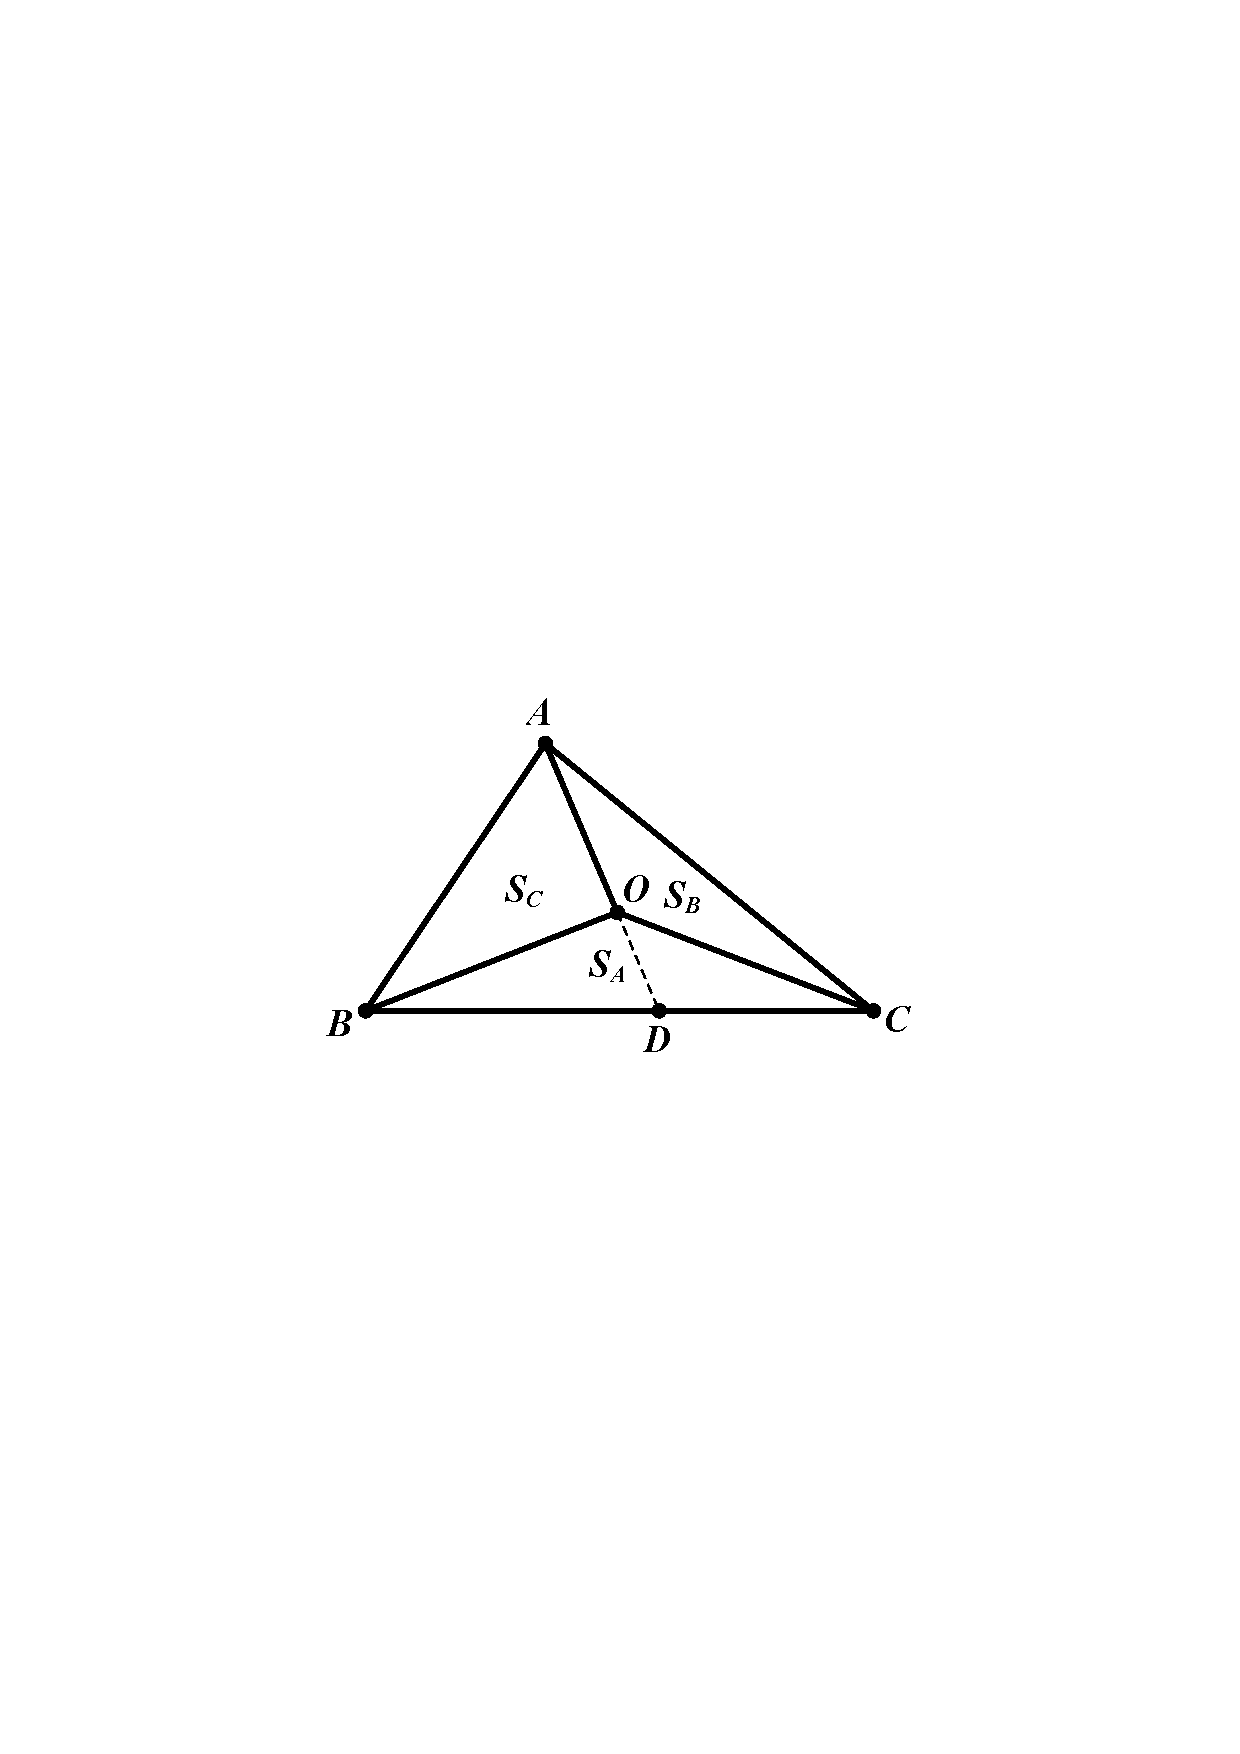
\includegraphics[width=0.3\linewidth]{内部点的向量和定理}
\end{figure}
延长$ AO $交$ BC $边于$ D $点,$ \dfrac{S_C}{S_B}=\dfrac{\frac{1}{2}AO\cdot BD \sin \angle  BDO}{\frac{1}{2}AO\cdot DC \sin \angle CDO}=\dfrac{BD}{DC} $,
\begin{gather*}
    \vec{OD}=\dfrac{DC}{BC}\cdot\vec{OB} + 
    \dfrac{BD}{BC}\cdot\vec{OC}=\dfrac{S_B}{S_B+S_C}\cdot
    \vec{OB} +\dfrac{S_C}{S_B+S_C}\cdot\vec{OC} \\
    \dfrac{OD}{OA}=\dfrac{S_{\Delta BOD}}{S_{\Delta BOA}}=
    \dfrac{S_{\Delta COD}}{S_{\Delta COA}}=\dfrac{S_{\Delta BOD}+
        S_{\Delta COD}}{S_{\Delta BOA}+S_{\Delta COA}}=\dfrac{S_A}{S_B+S_C} \\
    \vec{OD}=-\dfrac{S_A}{S_B+S_C}\cdot\vec{OA}=
    \dfrac{S_B}{S_B+S_C}\cdot
    \vec{OB} +\dfrac{S_C}{S_B+S_C}\cdot\vec{OC} \\
    S_A\cdot\vec{OA}+ S_B\cdot\vec{OB}
    +S_C\cdot\vec{OC}= \vec{0}
\end{gather*}
$\diamond$ 当$ O $是$ \Delta ABC $的重心时,
\begin{gather*}
    S_A:S_B:S_C=1:1:1\\  \vec{OA}
    +\vec{OB}+\vec{OC}=\vec{0}
\end{gather*}
$\diamond$ 当$ O $是$ \Delta ABC $的垂心时,
\begin{gather*}
    S_A:S_B:S_C=\tan A:\tan B:\tan C \\ \tan A\cdot
    \vec{OA}+\tan B\cdot \vec{OB}
    +\tan C\cdot\vec{OC}=\vec{0}
\end{gather*}
$\diamond$ 当$ O $是$ \Delta ABC $的内心时,
\begin{gather*}
    S_A:S_B:S_C=a:b:c \\ a\cdot \vec{OA}
    +b\cdot\vec{OB}+
    c\cdot\vec{OC}=\vec{0}
\end{gather*}
$\diamond$ 当$ O $是$ \Delta ABC $的外心时,
\begin{gather*}
    S_A:S_B:S_C=\sin 2A:\sin 2B:\sin 2C  \\
    \sin 2A\cdot\vec{OA}+ \sin 2B\cdot
    \vec{OB}+
    \sin 2C\cdot\vec{OC}=\vec{0}
\end{gather*}

\item (\ref{任意点面积定理})式可以推广到四面体中:设四面体$ A-BCD $内部有任意一点
$ O $,记$  O-ABC,O-ABD,O-ACD,O-BCD $的体积分别为$V_D,V_C,V_B,V_A $,那么有:
\begin{align*}
    V_A\cdot\vec{OA}+ V_B\cdot\vec{OB}
    +V_C\cdot\vec{OC}+V_D\cdot\vec{OD}= \vec{0}
\end{align*}

\item 设$ \Delta ABC $三个顶点的坐标分别为$ A(x_1,y_1),B(x_2,y_2),C(x_3,y_3) $,
平面上有一个动点$ P(x,y) $,考虑$ \lambda_1|PA|^2+\lambda_2|PB|^2+
\lambda_3|PC|^2 $的最小值,($ \lambda_1,\ \lambda_2,\ \lambda_3>0 $),
\begin{align*}
    &\ \lambda_1|PA|^2+\lambda_2|PB|^2+\lambda_3|PC|^2 \\
    =&\ (\lambda_1+\lambda_2+\lambda_3)x^2-2(\lambda_1x_1+\lambda_2x_2
    +\lambda_3x_3)x+\lambda_1x_1^2+\lambda_2x_2^2+\lambda_3x_3^2 \\ 
    +&\ (\lambda_1+\lambda_2+\lambda_3)y^2
    -2(\lambda_1y_1+\lambda_2y_2+\lambda_3y_3)y+
    \lambda_1y_1^2+\lambda_2y_2^2+\lambda_3y_3^2 \\
    =&\ (\lambda_1+\lambda_2+\lambda_3)\left(x-\dfrac{\lambda_1x_1+
        \lambda_2x_2+\lambda_3x_3}{\lambda_1
        +\lambda_2+\lambda_3}\right)^2+\cdots \\
    +&\ (\lambda_1+\lambda_2+\lambda_3)\left(y-\dfrac{\lambda_1y_1
        +\lambda_2y_2+\lambda_3y_3}{
        \lambda_1+\lambda_2+\lambda_3}\right)^2+ \cdots
\end{align*}
$ x,y $是两个完全独立的变量,所以,当$ x=\dfrac{\lambda_1x_1+\lambda_2x_2+
    \lambda_3x_3}{\lambda_1+\lambda_2+\lambda_3} $,$ y=\dfrac{\lambda_1y_1+
    \lambda_2y_2+\lambda_3y_3}{\lambda_1+\lambda_2+\lambda_3} $时,
$ \lambda_1|PA|^2+\lambda_2|PB|^2+\lambda_3|PC|^2 $取得极小值。\\
\ding{192} 当$ \lambda_1=\lambda_2=\lambda_3=1 $时,
\begin{gather*}
    x=\dfrac{x_1+x_2+x_3}{3},\q y=\dfrac{y_1+y_2+y_3}{3}
\end{gather*}
$ P $点是$ \Delta ABC $的重心。\\
\ding{193} 当$ \lambda_1=\tan A,\ \lambda_2=\tan B,\ \lambda_3=
\tan C $时,
\begin{align*}
    x &=\dfrac{(\tan A)x_1+(\tan B)x_2+(\tan C)x_3}{\tan A+\tan B+
        \tan C} \\ 
    y &=\dfrac{(\tan A)y_1+(\tan B)y_2+(\tan C)y_3}{\tan A+\tan B+
        \tan C}
\end{align*}
$ P $点是$ \Delta ABC $的垂心。\\
\ding{194} 当$ \lambda_1=\sin A,\ \lambda_2=\sin B,\ \lambda_3=
\sin C $时,
\begin{align*}
    x &=\dfrac{(\sin A)x_1+(\sin B)x_2+(\sin C)x_3}{\sin A+\sin B+
        \sin C}=\dfrac{ax_1+bx_2+cx_3}{a+b+c} \\ 
    y &=\dfrac{(\sin A)y_1+(\sin B)y_2+(\sin C)y_3}{\sin A+\sin B+
        \sin C}=\dfrac{ay_1+by_2+cy_3}{a+b+c}
\end{align*}
$ P $点是$ \Delta ABC $的内心。\\
\ding{195} 当$ \lambda_1=\sin 2A,\ \lambda_2=\sin 2B,\ \lambda_3=
\sin 2C $时,
\begin{align*}
    x &=\dfrac{(\sin 2A)x_1+(\sin 2B)x_2+(\sin 2C)x_3}{\sin 2A+
        \sin 2B+\sin 2C} \\
    y &=\dfrac{(\sin 2A)y_1+(\sin 2B)y_2+(\sin 2C)y_3}{\sin 2A+
        \sin 2B+\sin 2C}
\end{align*}
$ P $点是$ \Delta ABC $的外心。

\item 平面上有$ n $个不同的固定点$ A_1,A_2,\cdots,A_n $,
坐标为$ A_i(x_i,y_i)\ (i=1,2,\cdots,n) $,考虑动点$ P(x,y) $
到$ A_i $的距离的平方之和,
\begin{align*}
    S=&\ \sum_{i=1}^n \left[(x-x_i)^2+(y-y_i)^2\right] \\
    =&\ nx^2-2x\left(\sum_{i=1}^n x_i\right)+
    \left(\sum_{i=1}^n x_i^2\right)+ny^2-2y
    \left(\sum_{i=1}^n y_i\right)+
    \left(\sum_{i=1}^ny_i^2\right) \\
    =&\ n\left(x-\dfrac{1}{n}\sum_{i=1}^n x_i\right)^2+
    n\left(y-\dfrac{1}{n}\sum_{i=1}^n y_i\right)^2 \\
    &\ -\dfrac{1}{n}\left(\sum_{i=1}^n x_i\right)^2+
    \left(\sum_{i=1}^n x_i^2\right)
    -\dfrac{1}{n}\left(\sum_{i=1}^n y_i\right)^2+
    \left(\sum_{i=1}^n y_i^2\right)
\end{align*}
观察上式可以得出两个结论:\\
(一) 当$ x=\dfrac{1}{n}\sum\limits_{i=1}^n x_i,\ 
y=\dfrac{1}{n}\sum\limits_{i=1}^n y_i $时,$ S $取得最小值。\\
(二) 如果$ S $是定值,那么$ P $点的轨迹如果存在,则是一个圆。

\item $^*$ 设$ P $是$ \Delta ABC $内的一点,从$ P $点向三条边分别作垂线,
垂足分别为$ D,E,F $,则有Erdos-Mordell不等式\footnote{证明参见
https://forumgeom.fau.edu/FG2007volume7/FG200711.pdf }:
\begin{gather*}
    |PA|+|PB|+|PC|\geq 2(|PD|+|PE|+|PF|)
\end{gather*}
当$ P $是$ \Delta ABC $的外心时,等号成立。

\item 对于$ \Delta ABC $,分别以$ AB,BC,AC $为边,
在$ \Delta ABC $外部作三个等边三角形,
这三个等边三角形的外接圆会交于同一点,该交点被称为\textbf{费马点}
(也称\textbf{托里拆利点})。
\begin{itemize}[itemsep=-3pt]
\item 如果三角形的最大内角小于$ 120^{\circ} $,那么费马点位于
$ \Delta ABC $内部,且费马点(记为$ P $点)就是使到三角形三个顶点距离之和
取最小值的点,$ PA,PB,PC $恰好互成$ 120^{\circ} $.
(证明见本书第\pageref{费马点求偏导}页);
\item 如果三角形的最大内角等于$ 120^{\circ} $,则费马点位于钝角顶点;
\item 如果三角形的最大内角大于$ 120^{\circ} $,则费马点位于$ \Delta ABC $
外部;
\end{itemize}
对于后两种情形(最大内角大于等于$ 120^{\circ} $),钝角顶点是到三个顶点
距离之和最小的点。有些参考资料中把最后一种情形下的钝角顶点
(而不是外接圆交点)称为费马点,这是不恰当的。
\begin{figure}[!h]
    \centering
    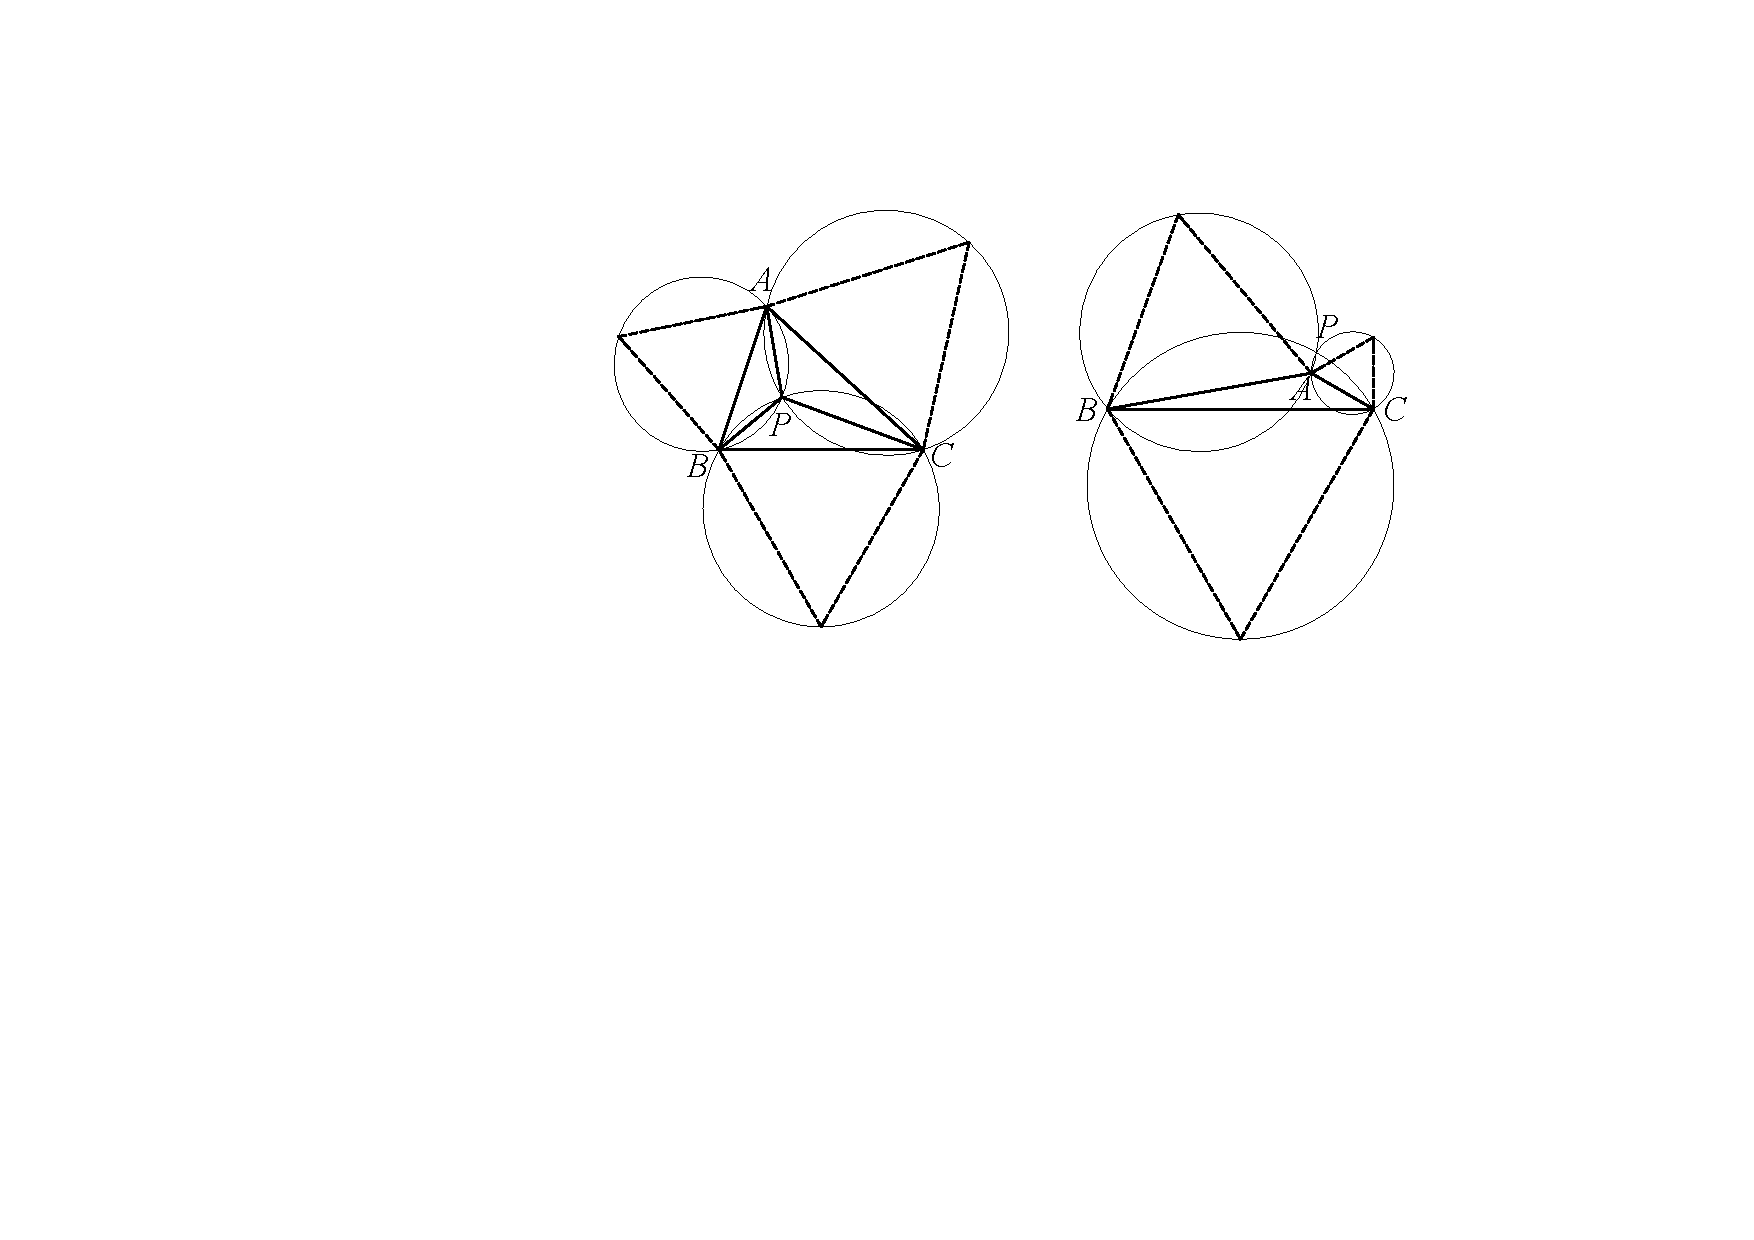
\includegraphics[width=0.8\linewidth]{费马点-朝外作三角形}
    \label{费马点朝内朝外两种}
\end{figure}

如果三个等边三角形不是全部在$ \Delta ABC $外部,而是全部在与
$ \Delta ABC $有相交区域的方位(或者说向内部作等边三角形),
三个外接圆也会交于同一点,且交点位于$ \Delta ABC $外部,
此时的交点不具备与三个顶点距离之和最小的特点。
\begin{figure}[!h]
    \centering
    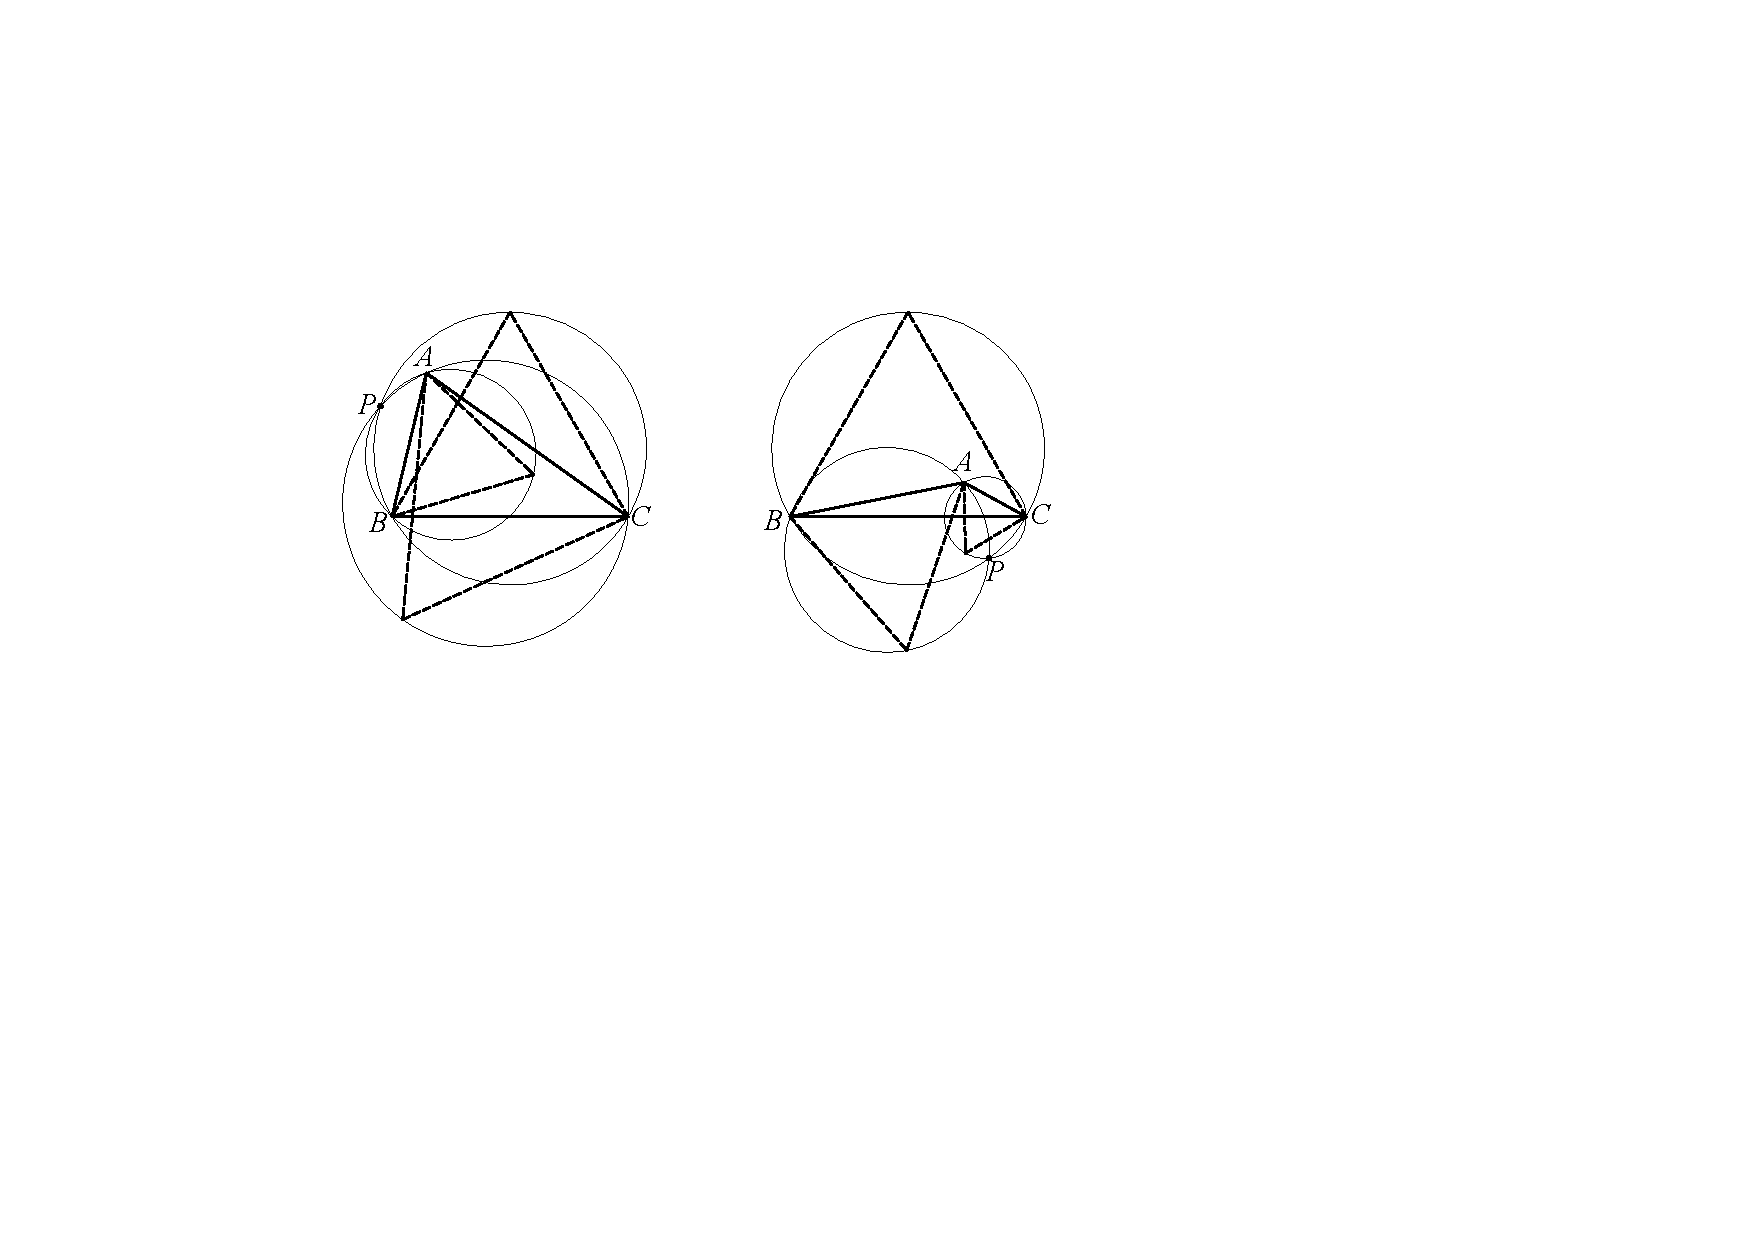
\includegraphics[width=0.8\linewidth]{费马点-朝内作三角形}
\end{figure}
\newpage

\end{itemize}

\section{三角形中的等式与不等式}
\begin{itemize}[leftmargin=\inteval{\myitemleftmargin}pt,itemsep=
    \inteval{\myitemitempsep}pt,topsep=\inteval{\myitemtopsep}pt]
    \item $ \Delta ABC $中的恒等式($ A+B+C=\pi $)
    \begin{align} 
        &\sin A +\sin B +\sin C =4\cos\Big(\dfrac{A}{2}\Big)
        \cos\Big(\dfrac{B}{2}\Big)\cos\Big(\dfrac{C}{2}\Big) \label{三角恒等式1} \\
        &\sin2A +\sin2B +\sin2C =4\sin A  \sin B \sin C \label{三角恒等式2}\\
        &\cos A +\cos B +\cos C =1+4\sin\Big(\dfrac{A}{2}\Big)
        \sin\Big(\dfrac{B}{2}\Big)\sin\Big(\dfrac{C}{2}\Big) \label{三角恒等式3} \\
        &\cos2A +\cos2B +\cos2C =-1-4\cos A\cos B \cos C \label{三角恒等式4} \\	
        &\cos^2A+\cos^2B+\cos^2C =1-2\cos A\cos B\cos C \label{三角恒等式5} \\ 
        &\sin^2A+\sin^2B+\sin^2C =2+2\cos A\cos B\cos C \label{三角恒等式6} \\
        &\tan A+\tan B +\tan C =\tan A \tan B\tan C \label{三角恒等式7}\\
        &\cot A\cot B+\cot B \cot C+\cot A\cot C=1 \label{三角恒等式8}\\
        &\tan\Big(\dfrac{A}{2}\Big)\tan\Big(\dfrac{B}{2}\Big)+
        \tan\Big(\dfrac{B}{2}\Big)\tan\Big(\dfrac{C}{2}\Big)+
        \tan\Big(\dfrac{A}{2}\Big)\tan\Big(\dfrac{C}{2}\Big)=1 \label{三角恒等式-最后}
    \end{align}
    
    \item 从左到右证明(\ref{三角恒等式1})式,使用和差化积公式:
    \begin{align*}
        & (\sin A +\sin B) +\sin C  \\
        =&\  2\sin\left(\dfrac{A+B}{2}\right)\cos\left(\dfrac{A-B}{2}\right)+\sin(A+B) \\    
        =&\  2\sin\left(\dfrac{A+B}{2}\right)\cos\left(\dfrac{A-B}{2}\right)+
        2\sin\left(\dfrac{A+B}{2}\right)\cos\left(\dfrac{A+B}{2}\right) \\
        =&\  2\sin\left(\dfrac{A+B}{2}\right)\cdot 2\cos\left(\dfrac{A}{2}\right)\cos\left(\dfrac{B}{2}\right) \\
        =&\  4\cos\left(\dfrac{C}{2}\right)\cos\left(\dfrac{A}{2}\right)\cos\left(\dfrac{B}{2}\right)
    \end{align*}
    \item 从右到左证明(\ref{三角恒等式1})式,
    \begin{align*}
        & 4\cos\left(\dfrac{A}{2}\right)\cos\left(\dfrac{B}{2}\right)\sin\left(\dfrac{A+B}{2}\right) \\
        =&\  4\cos\left(\dfrac{A}{2}\right)\cos\left(\dfrac{B}{2}\right) \left[\sin\left(\dfrac{A}{2}\right) \cos\left(\dfrac{B}{2}\right)+\cos\left(\dfrac{A}{2}\right) \sin\left(\dfrac{B}{2}\right) \right] \\
        =&\  4\cos\left(\dfrac{A}{2}\right)\sin\left(\dfrac{A}{2}\right)\cos^2\left(\dfrac{B}{2}\right)+
        4\cos\left(\dfrac{B}{2}\right)\sin\left(\dfrac{B}{2}\right)\cos^2\left(\dfrac{A}{2}\right)\\
        =&\  \sin A (\cos B+1)+\sin B(\cos A +1) \\
        =&\  \sin A +\sin B + \sin(A+B)
    \end{align*}
    以上方法同样适用于(\ref{三角恒等式2}),(\ref{三角恒等式3}),(\ref{三角恒等式4}).
    由(\ref{三角恒等式4})式可以导出(\ref{三角恒等式5})式,
    由(\ref{三角恒等式5})式可以导出(\ref{三角恒等式6})式。
    由(\ref{三角恒等式6})式可知$ \cos A\cos B\cos C >-1 $,
    由(\ref{三角恒等式3})式可知$ \cos A+\cos B+\cos C >1 $.  
    
    \item 由$ \tan(A+B)=\dfrac{\tan A+\tan B}{1-\tan A\tan B}=
    \tan(\pi-C)=-\tan C $可得到(\ref{三角恒等式7})式,
    (\ref{三角恒等式7})式两边同除$ \tan A \tan B\tan C $可得到(\ref{三角恒等式8})式。
    由$ \tan\Big(\dfrac{A}{2}+\dfrac{B}{2}\Big)=\dfrac{\tan \dfrac{A}{2}+
        \tan \dfrac{B}{2}}{1-\tan \dfrac{A}{2}\tan \dfrac{B}{2}}
    =\tan\Big(\dfrac{\pi}{2}-\dfrac{C}{2}\Big)=\dfrac{1}{\tan \dfrac{C}{2}} $
    可得到(\ref{三角恒等式-最后})式。
    
    \item 对任意$ \Delta ABC $,有如下不等式成立:
    \begin{gather}
        0<\sin A +\sin B +\sin C \leq \frac{3\sqrt{3}}{2} \label{sinA+sinB+sinC}\\    
        0<\sin A \sin B \sin C \leq \frac{3\sqrt{3}}{8} \label{sinAsinBsinC}\\
        1<\cos A +\cos B +\cos C \leq \frac{3}{2} \label{cosA+cosB+cosC}\\
        -1<\cos A\cos B\cos C \leq \frac{1}{8} \label{cosAcosBcosC}
    \end{gather}
    右侧不等号中的等号均在$ A=B=C=\dfrac{\pi}{3} $时取得,左侧则是至少一个角趋于0时的极限
    (剩余两个角可能趋于$ 0 $和$ \pi $,也可能都趋于$ \dfrac{\pi}{2} $).
    
    \item (\ref{sinA+sinB+sinC})式左侧不等式显然成立,现证明右侧。\\
    \textbf{方法一}\ 利用正弦函数$ y=\sin x $在$ [0,\pi] $上的凹凸性
    (不等式(\ref{琴森不等式})):
    \begin{gather*}
        \sin A +\sin B +\sin C \leq 3\sin \dfrac{A+B+C}{3}=\dfrac{3\sqrt{3}}{2}
    \end{gather*}
    \textbf{方法二}\ 考虑$ y=\sin x $在$ \Big(\dfrac{\pi}{3},\dfrac{\sqrt{3}}{2}
    \Big) $处的切线$ y=\dfrac{1}{2}\Big(x-\dfrac{\pi}{3}\Big)+\dfrac{\sqrt{3}}{2} $,
    $ \forall x\in [0,\pi] $,有$ \sin x\leq \dfrac{1}{2}\Big(x-\dfrac{\pi}{3}\Big)
    +\dfrac{\sqrt{3}}{2} $,所以,
    \begin{gather*}
        \sin A +\sin B +\sin C \leq \dfrac{1}{2}\Big(A+B+C-3\cdot\dfrac{\pi}{3}\Big)
        +3\cdot\dfrac{\sqrt{3}}{2}=\dfrac{3\sqrt{3}}{2}
    \end{gather*}
    \textbf{方法三}\ 利用均值不等式(\ref{完整的均值不等式})、(\ref{三角恒等式6})式、
    (\ref{cosAcosBcosC})式:
    \begin{align*}
        \sin A +\sin B +\sin C \leq &\ \sqrt{3(\sin^2A+\sin^2B+\sin^2C)} \\
        =&\ \sqrt{3(2+2\cos A\cos B\cos C)}\leq \sqrt{3\left(2+2\cdot 
            \dfrac{1}{8}\right)}=\dfrac{3\sqrt{3}}{2}
    \end{align*}
    
    \item (\ref{sinAsinBsinC})式左侧不等式显然成立,现证明右侧。利用均值不等式
    (\ref{完整的均值不等式}):
    \begin{gather}
        \sin A \sin B \sin C \leq \left(\dfrac{\sin A +\sin B +\sin C}{3} \right)^3
        \leq \left(\dfrac{\sqrt{3}}{2}\right)^3=\dfrac{3\sqrt{3}}{8}
        \label{三个正弦和不等式-小于}
    \end{gather}
    
    \item 证明(\ref{cosA+cosB+cosC})式。\\
    \textbf{方法一}\ 利用(\ref{三角恒等式3})式、均值不等式和正弦函数的凹凸性:
    \begin{align}
        \cos A +\cos B +\cos C =&\ 1+4\sin\Big(\dfrac{A}{2}\Big)
        \sin\Big(\dfrac{B}{2}\Big)\sin\Big(\dfrac{C}{2}\Big)\qquad (>1) \nonumber \\
        \leq &\ 1+4\left[\dfrac{\sin(\frac{A}{2})+
            \sin(\frac{B}{2})+\sin(\frac{C}{2})}{3}\right]^3 \nonumber \\
        \leq &\ 1+ 4\left(\sin \dfrac{\frac{A}{2}+\frac{B}{2}+\frac{C}{2}}{3}\right)^3=
        1+4\left(\dfrac{1}{2}\right)^3=\dfrac{3}{2} \label{三个余弦和不等式-小于}
    \end{align}
    \textbf{方法二}\ 考虑$ y=\cos x $在$ \Big(\dfrac{\pi}{3},\dfrac{1}{2}
    \Big) $处的切线$ y=-\dfrac{\sqrt{3}}{2}\Big(x-\dfrac{\pi}{3}\Big)+\dfrac{1}{2} $,
    $ \forall x\in [0,\pi] $,有$ \cos x\leq -\dfrac{\sqrt{3}}{2}\Big(x-
    \dfrac{\pi}{3}\Big)+\dfrac{1}{2} $,所以,
    \begin{gather*}
        \cos A +\cos B +\cos C \leq -\dfrac{\sqrt{3}}{2}\Big(A+B+C-3\cdot
        \dfrac{\pi}{3}\Big)+3\cdot\dfrac{1}{2}=\dfrac{3}{2}
    \end{gather*}
    
    \item 对于(\ref{cosAcosBcosC})式,因为$ |\cos A\cos B\cos C|<1 $,
    所以$ \cos A\cos B\cos C>-1 $,左侧成立。现证明(\ref{cosAcosBcosC})式右侧成立。\\
    \textbf{方法一}\ 利用均值不等式:
    \begin{gather*}
        \cos A \cos B \cos C \leq \left(\dfrac{\cos A +\cos B +\cos C}{3} \right)^3
        \leq \left(\dfrac{1}{2}\right)^3=\dfrac{1}{8}
    \end{gather*}
    \textbf{方法二}\ 利用(\ref{三角恒等式5})式和均值不等式,
    \begin{align*}
        1-2\cos A\cos B\cos C=\cos^2A+\cos^2B+\cos^2C \geq 3(\cos A\cos B\cos C)^{2/3}
    \end{align*}
    记$ t=(\cos A\cos B\cos C)^{1/3} $,那么 $ 2t^3+3t^2-1= (2t-1)(t+1)^2 \leq 0 $,
    于是$ t\leq \dfrac{1}{2} $,$ \cos A\cos B \cos C=t^3\leq \dfrac{1}{8} $.  
    
    \item 当$ x\in\Big(0,\dfrac{\pi}{2}\Big) $时,
    $ \sin x>\dfrac{2}{\pi}x $,$ \cos x>1-\dfrac{2}{\pi}x $.
    \begin{figure}[!h]  % sinx_Great_2x_pi.m
        \centering
        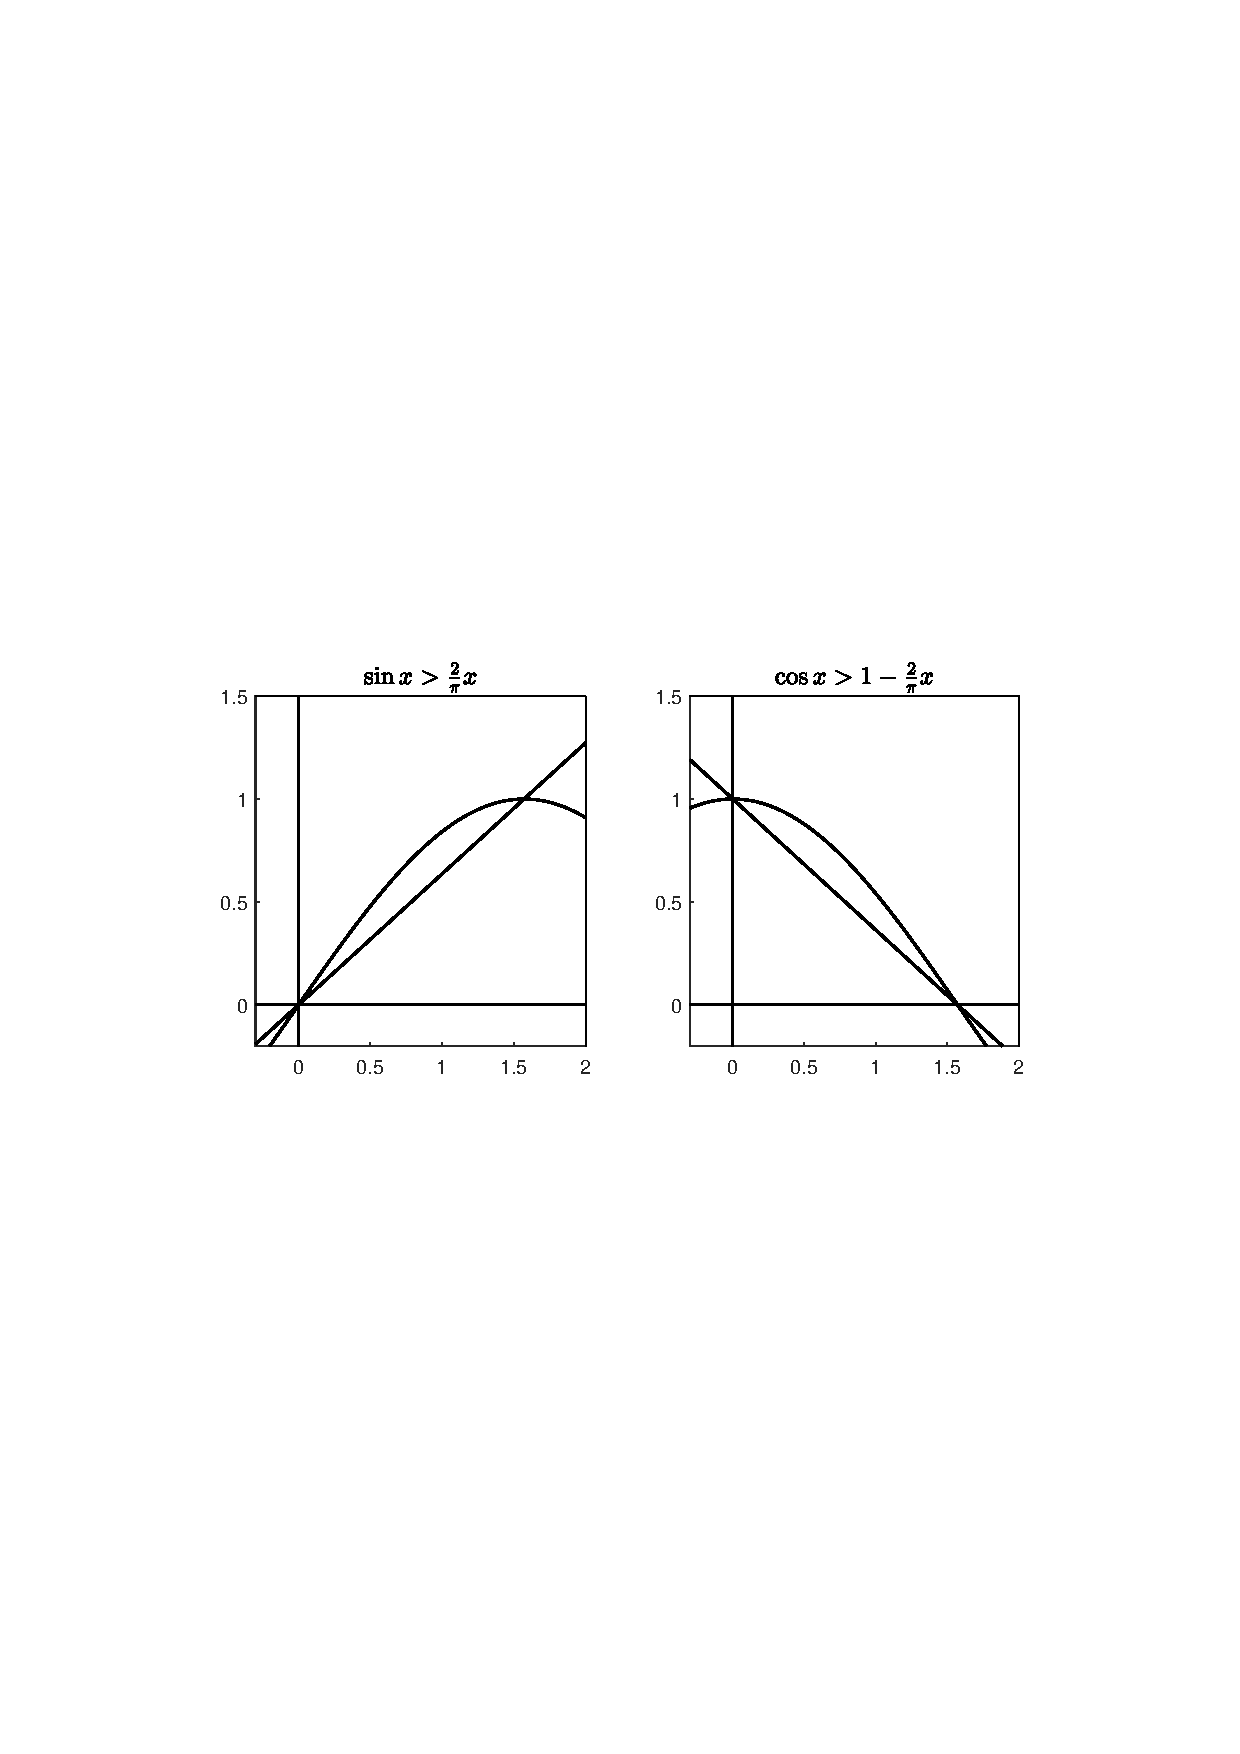
\includegraphics[width=0.7\linewidth]{sinx大于2x_pi}
    \end{figure} \\
    对于锐角三角形$ ABC $,有
    \begin{align*}
        \sin A +\sin B +\sin C &>\dfrac{2}{\pi}(A+B+C)=2 \\
        \cos A +\cos B +\cos C &>3-\dfrac{2}{\pi}(A+B+C)=1
    \end{align*}
    
    \item 若$ \Delta ABC $是钝角三角形,那么$ \tan A+\tan B +\tan C =
    \tan A \tan B\tan C <0 $.\\
    若$ \Delta ABC $是锐角三角形,那么
    \begin{gather*}
        \tan A+\tan B +\tan C =\tan A \tan B\tan C \leq \left(
        \dfrac{\tan A+\tan B +\tan C}{3}\right)^3
    \end{gather*}
    于是
    \begin{gather*}
        \tan A+\tan B +\tan C\geq 3\sqrt{3}
    \end{gather*}
    也可以从正切函数的凹凸性来理解上式,
    \begin{gather*}
        \tan A+\tan B +\tan C\geq 3\tan\dfrac{A+B+C}{3}=3\sqrt{3}
    \end{gather*}
    或者考虑$ y=\tan x $在$ \Big(\dfrac{\pi}{3},\sqrt{3}\Big) $
    处的切线$ y=4\Big(x-\dfrac{\pi}{3}\Big)+\sqrt{3} $,
    $ \forall x\in \Big[0,\dfrac{\pi}{2}\Big) $,有$ \tan x\geq 
    4\Big(x-\dfrac{\pi}{3}\Big)+\sqrt{3} $,所以,
    \begin{gather*}
        \tan A +\tan B +\tan C \geq 4\Big(A+B+C-3\cdot\dfrac{\pi}{3}\Big)
        +3\sqrt{3}=3\sqrt{3}
    \end{gather*}
    
\end{itemize}

\section{一些平面几何的定理}
\begin{itemize}[leftmargin=\inteval{\myitemleftmargin}pt,itemsep=
   \inteval{\myitemitempsep}pt,topsep=\inteval{\myitemtopsep}pt]
\item 三角形的内角平分线定理:$ \dfrac{|AB|}{|AC|}=
\dfrac{|BD|}{|CD|} $的充分必要条件是:
$ AD $是$ \angle BAC $的角平分线。(提示,$ |DE|=|DF| $,考虑
$ \Delta ABD $与$ \Delta ACD $的面积之比。)
\begin{figure}[!h]
    \centering
    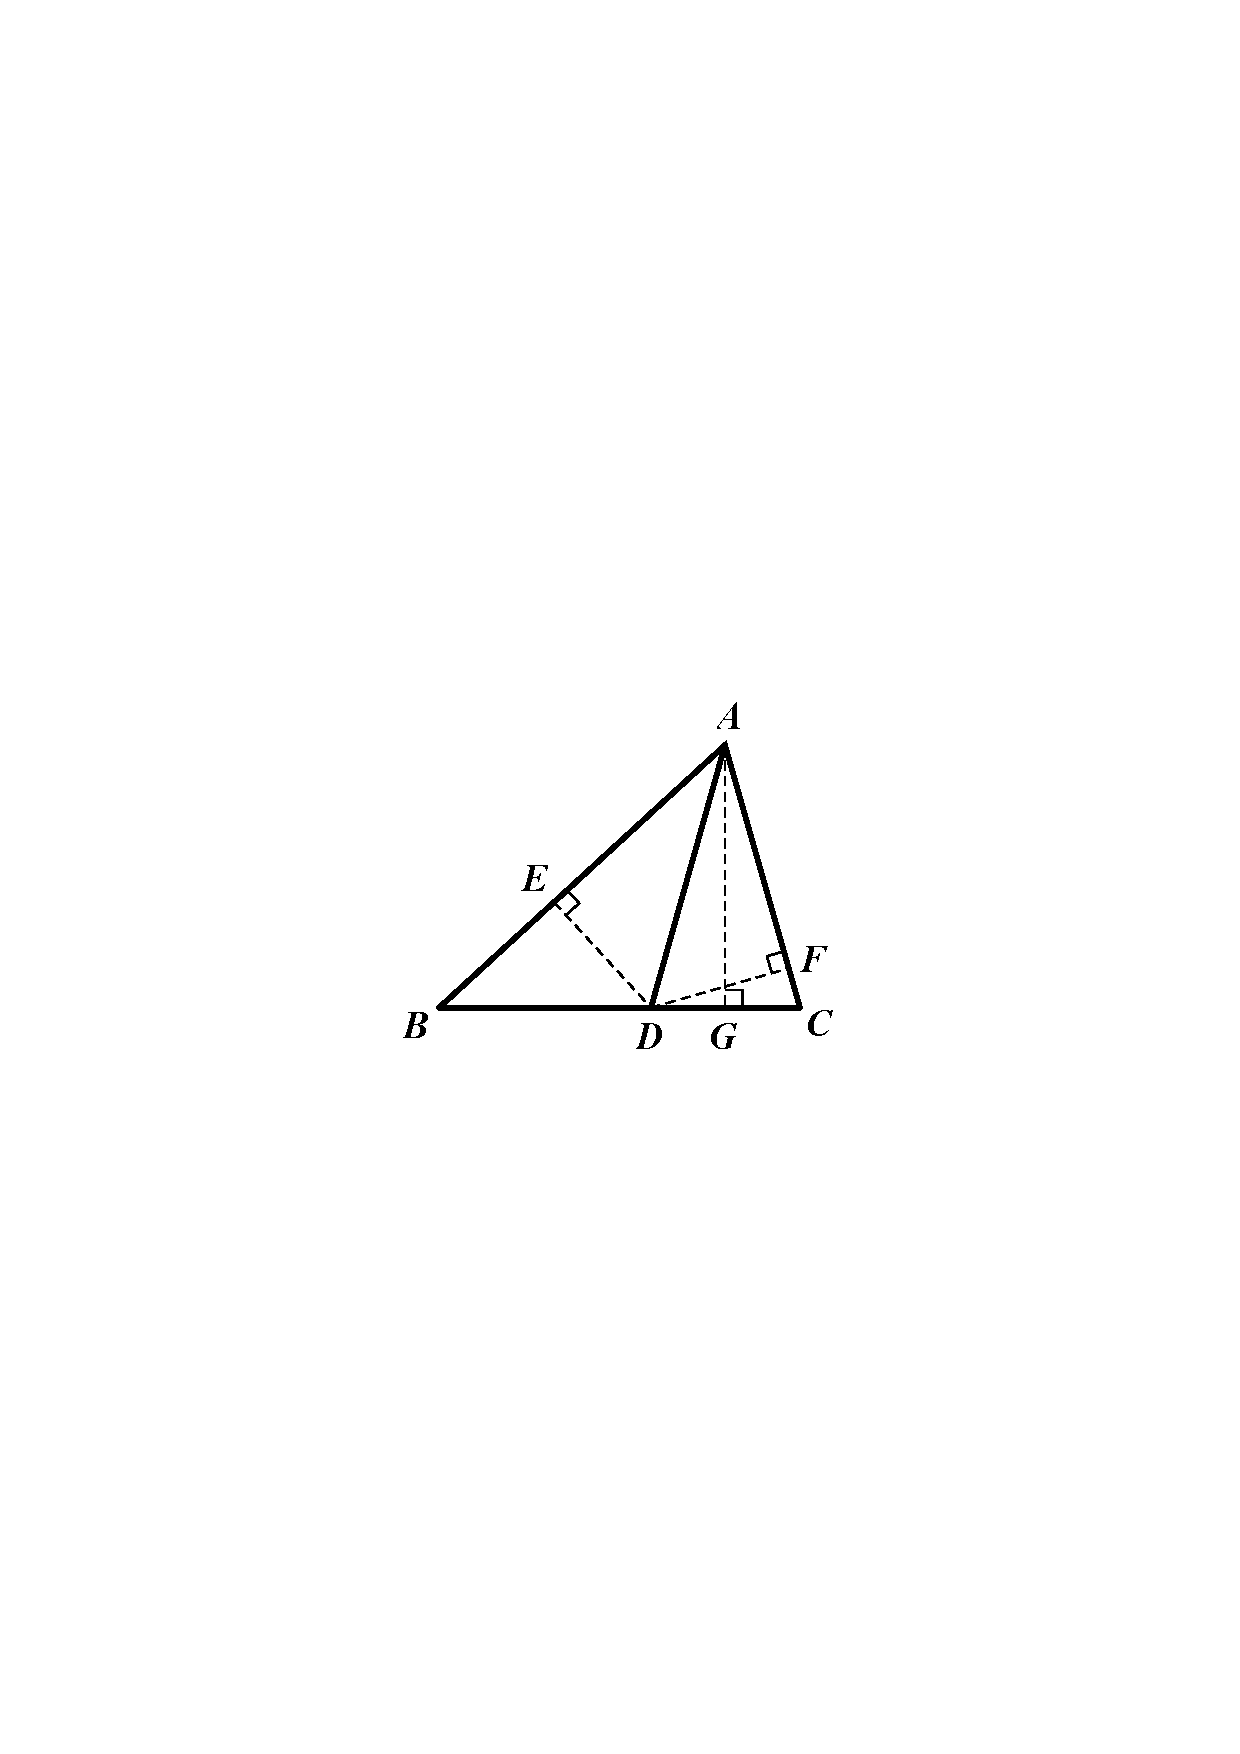
\includegraphics[width=0.3\linewidth]{三角形的内角平分线定理}
\end{figure} 

\item 梅涅劳斯定理$ ^* $:直线$ l $与$ \Delta ABC $的三边所在直线
分别交于$ D,E,F $点,则有
\begin{gather*}
    \dfrac{|AD|}{|DB|} \cdot \dfrac{|BE|}{|EC|} \cdot
    \dfrac{|CF|}{|FA|}=1
\end{gather*}
\begin{figure}[h]
    \centering
    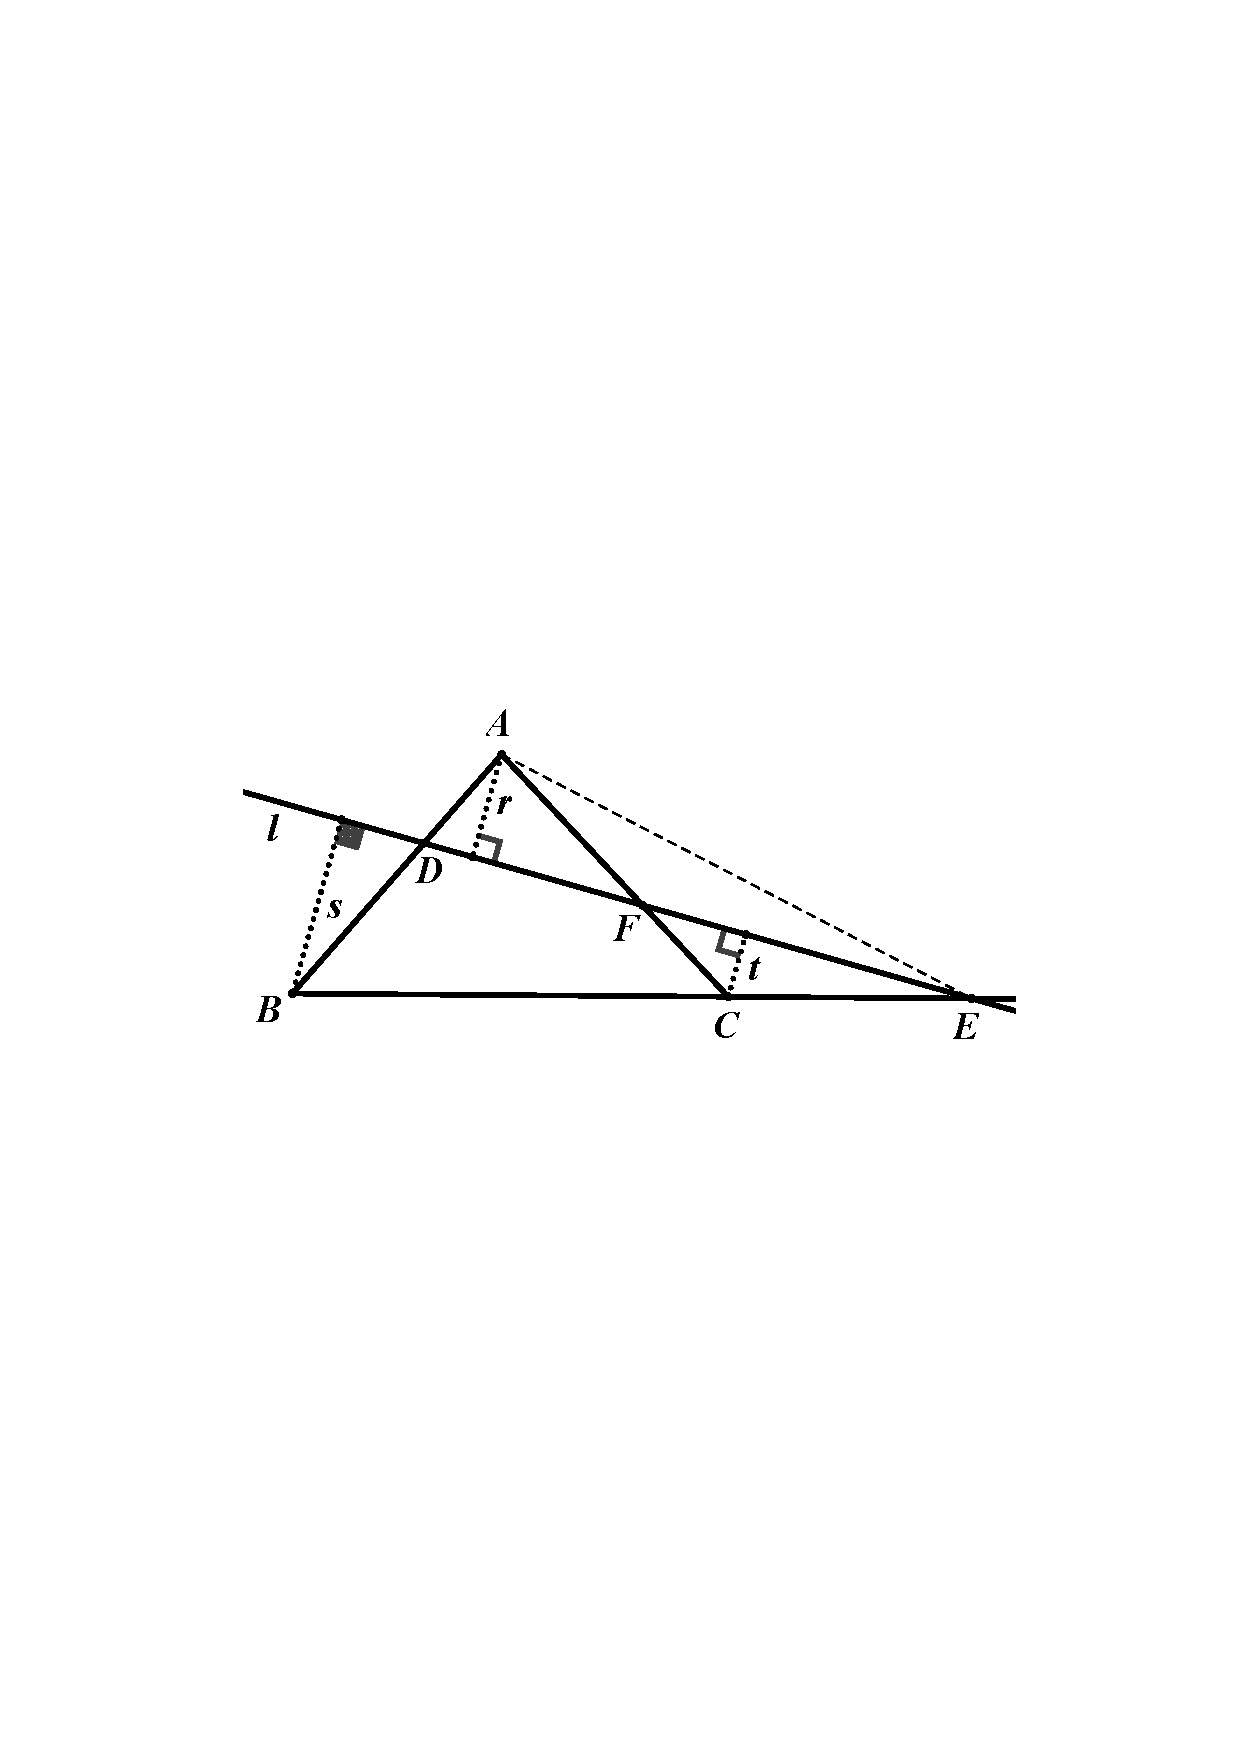
\includegraphics[width=0.5\linewidth]{梅涅劳斯定理}
\end{figure} \\
\textbf{方法一}\ 
\begin{gather*}
    \dfrac{S_{\Delta ADF}}{S_{\Delta BDE}}=\dfrac{|AD|\cdot|DF|}{|DB|\cdot|DE|},\quad
    \dfrac{S_{\Delta BDE}}{S_{\Delta CFE}}=\dfrac{|BE|\cdot|DE|}{|EC|\cdot|EF|},\quad
    \dfrac{S_{\Delta CFE}}{S_{\Delta ADF}}=\dfrac{|CF|\cdot|EF|}{|FA|\cdot|DF|} \\
    \dfrac{S_{\Delta ADF}}{S_{\Delta BDE}}\cdot\dfrac{S_{\Delta BDE}}{S_{\Delta CFE}}
    \cdot\dfrac{S_{\Delta CFE}}{S_{\Delta ADF}}=\dfrac{|AD|}{|DB|} \cdot
    \dfrac{|BE|}{|EC|} \cdot \dfrac{|CF|}{|FA|}=1
\end{gather*}
\textbf{方法二}\ 分别从$ A,B,C $向$ l $作垂线,垂线段的长度依次为$ r,s,t $,则
\begin{align*}
    \dfrac{|AD|}{|DB|} \cdot	\dfrac{|BE|}{|EC|} \cdot \dfrac{|CF|}{|FA|}=
    \dfrac{r}{s} \cdot \dfrac{s}{t} \cdot \dfrac{t}{r}= 1
\end{align*}
\textbf{方法三}\ 设$ \vec{AD}=k_1\vec{AB},\ \vec{AF}=
k_2\vec{AC},\ k_1\neq k_2 $,因为$ D,F,E $三点共线,那么
\begin{gather*}
    \vec{AE}=\lambda \vec{AD}+(1-\lambda)\vec{AF}=
    \lambda k_1\vec{AB}+(1-\lambda)k_2\vec{AC}
\end{gather*}
又因为$ B,C,E $三点共线,所以$ \lambda k_1+(1-\lambda)k_2=1,\ \lambda=\dfrac{1-k_2}
{k_1-k_2} $,$ \dfrac{|BE|}{|EC|} =-\dfrac{(1-\lambda)k_2}{\lambda k_1} =
\dfrac{k_2(1-k_1)}{k_1(1-k_2)} $,
\begin{align*}
    \dfrac{|AD|}{|DB|} \cdot	\dfrac{|BE|}{|EC|} \cdot \dfrac{|CF|}{|FA|}=
    \dfrac{k_1}{1-k_1}\cdot \dfrac{k_2(1-k_1)}{k_1(1-k_2)}\cdot\dfrac{1-k_2}{k_2}=1
\end{align*}

\item 塞瓦定理$ ^* $:$ \Delta ABC $内部任取一点$ P $,连接$ AP $并延长,交$ BC $
于$ E $点,连接$ BP $并延长,交$ CA $于$ F $点,连接$ CP $并延长,交$ AB $于$ D $点,
则有$ \dfrac{|AD|}{|DB|} \cdot \dfrac{|BE|}{|EC|} \cdot\dfrac{|CF|}{|FA|}=1 $. 
\begin{figure}[H]
    \centering
    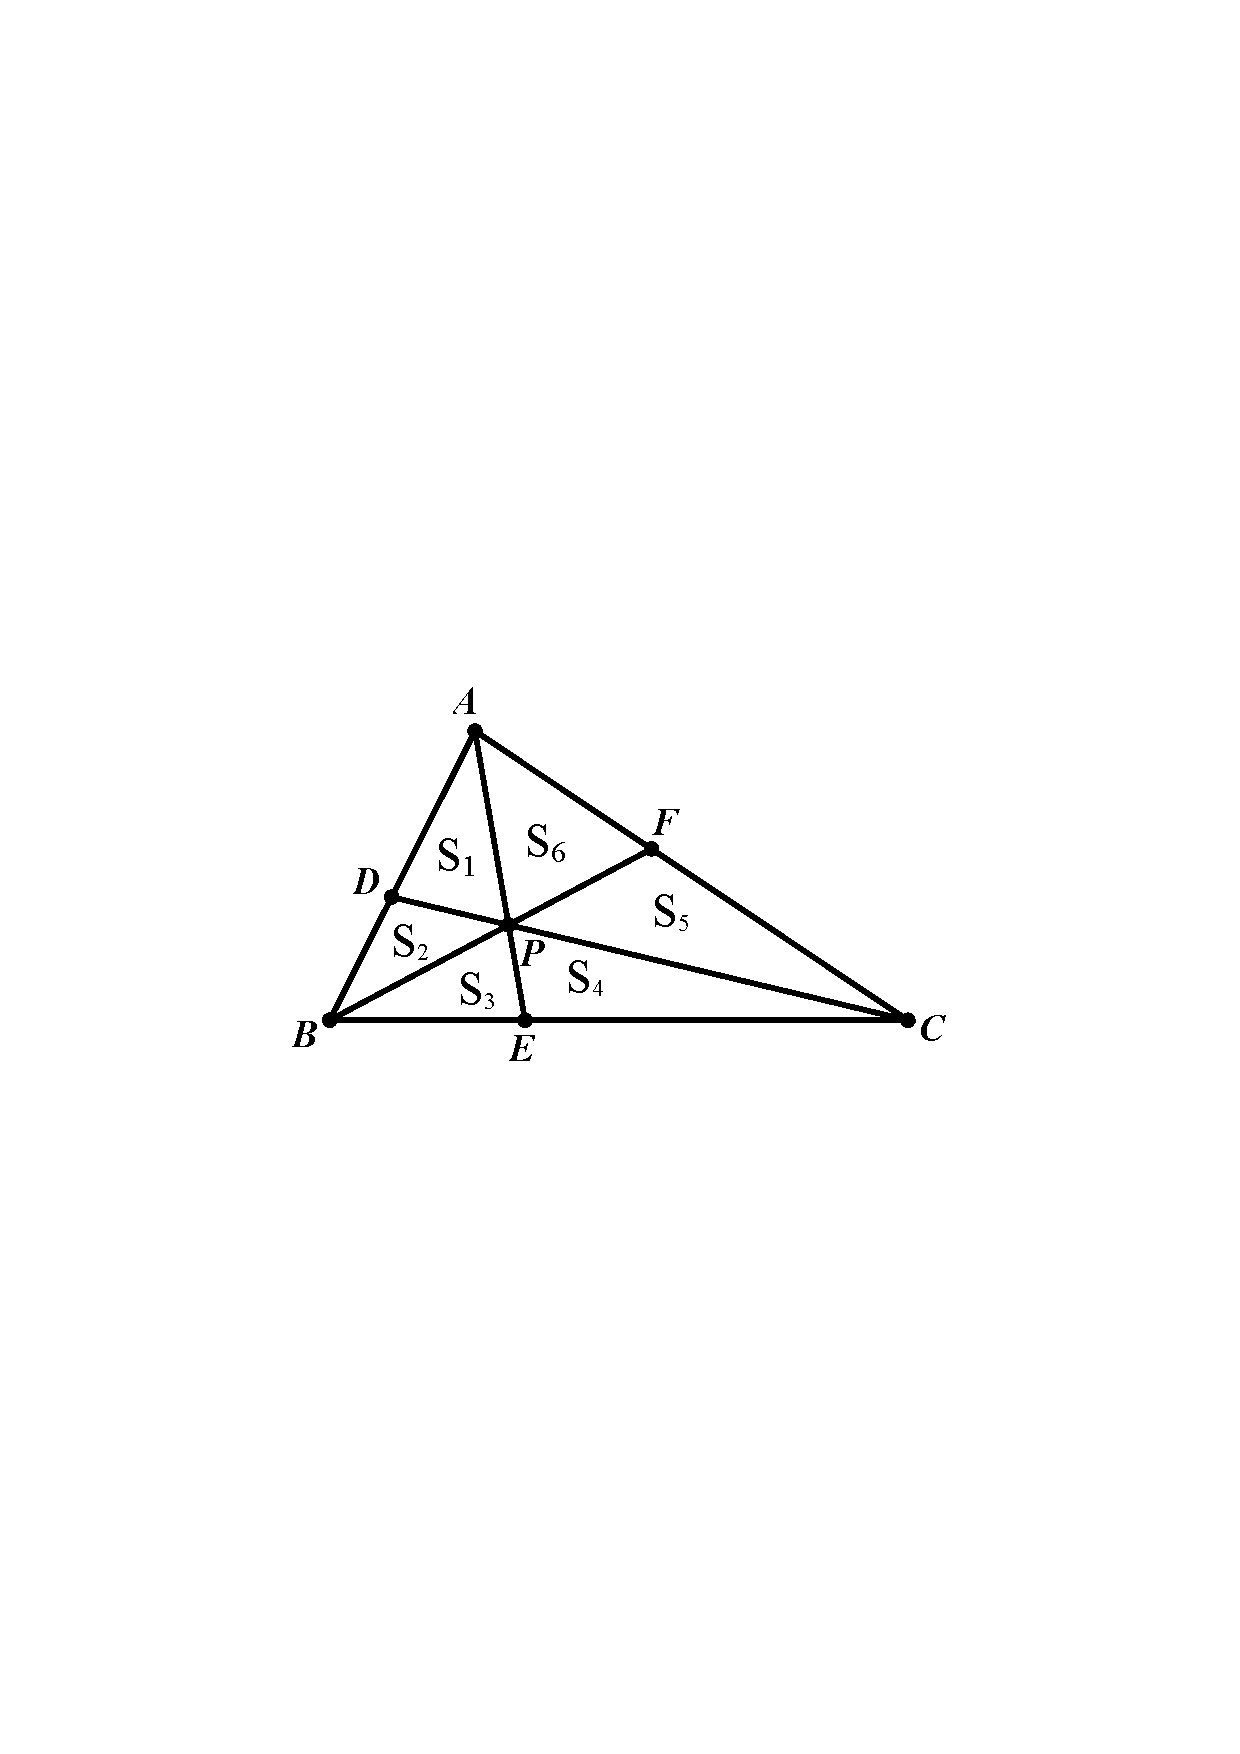
\includegraphics[width=0.5\linewidth]{塞瓦定理}
\end{figure}
\textbf{方法一}\ 设$ \Delta APD,\Delta BPD,\Delta BPE,\Delta CPE,
\Delta CPF,\Delta APF $的面积分别为$S_1$,$S_2$,$S_3$,
$S_4$,$S_5$,$S_6$,则
\begin{gather*}
    \dfrac{|BE|}{|EC|}=\dfrac{S_3}{S_4}=\dfrac{S_1+S_2+S_3}{S_4+S_5+S_6}=
    \dfrac{S_1+S_2}{S_5+S_6}		\\
    \dfrac{|AD|}{|DB|} \cdot \dfrac{|BE|}{|EC|} \cdot\dfrac{|CF|}{|FA|}=
    \dfrac{S_5+S_6}{S_3+S_4} \cdot \dfrac{S_1+S_2}{S_5+S_6} \cdot \dfrac{S_3+S_4}{S_1+S_2} =1
\end{gather*} 
\textbf{方法二}\ 设$ \vec{AD}=k_1\vec{AB},\ \vec{AF}=
k_2\vec{AC} $,那么
\begin{align*}
    \vec{AP}=&\ \lambda \vec{AD}+(1-\lambda)\vec{AC}=
    \mu \vec{AF}+(1-\mu)\vec{AB} \\
    =&\ \lambda k_1\vec{AB}+(1-\lambda)\vec{AC}=
    \mu k_2\vec{AC}+(1-\mu)\vec{AB}
\end{align*}
所以,$ \lambda k_1=1-\mu,\ 1-\lambda=\mu k_2 $,解得:$ \lambda=\dfrac{1-k_2}{1-k_1k_2},
\ \mu=\dfrac{1-k_1}{1-k_1k_2} $,$ \dfrac{|BE|}{|EC|} =\dfrac{1-\lambda}{\lambda k_1} =
\dfrac{k_2(1-k_1)}{k_1(1-k_2)} $,
于是
\begin{align*}
    \dfrac{|AD|}{|DB|} \cdot \dfrac{|BE|}{|EC|} \cdot\dfrac{|CF|}{|FA|}=
    \dfrac{k_1}{1-k_1}\cdot \dfrac{k_2(1-k_1)}{k_1(1-k_2)}\cdot\dfrac{1-k_2}{k_2}=1
\end{align*}

\item 托勒密定理$ ^* $:圆的内接四边形两组对边乘积的和等于两条对角线的乘积。\\
\textbf{方法一}\ 圆的半径不影响本题结论的成立与否。设单位圆上不同的四点的坐标为 \\
$ (\cos \alpha_k,\sin \alpha_k)(k=1,2,3,4) $,适当的坐标系选取可保证
$ 0< \alpha_1 <\alpha_2<\alpha_3<\alpha_4<2\pi $,只需验证下式:
\begin{align*}
    \sin\dfrac{\alpha_2-\alpha_1}{2}\cdot 
    \sin\dfrac{\alpha_4-\alpha_3}{2}+\sin\dfrac{\alpha_4-\alpha_1}{2}\cdot
    \sin\dfrac{\alpha_3-\alpha_2}{2}=\sin\dfrac{\alpha_3-\alpha_1}{2}\cdot 
    \sin\dfrac{\alpha_4-\alpha_2}{2}
\end{align*}
\textbf{方法二}\ 设四边形的四个顶点对应的复数分别为$ z_1,z_2,z_3,z_4 $,有恒等式
\begin{align*}
    (z_1-z_2)(z_3-z_4)+(z_1-z_4)(z_2-z_3)=(z_1-z_3)(z_2-z_4)
\end{align*}
在这个等式两边取模,有
\begin{align*}
    |(z_1-z_2)(z_3-z_4)|+|(z_1-z_4)(z_2-z_3)|\geq &\  \\
    |(z_1-z_2)(z_3-z_4)+(z_1-z_4)(z_2-z_3)|=&\ |(z_1-z_3)(z_2-z_4)|
\end{align*}
等号成立的条件是四点共圆或者四点共线。

\item 横纵坐标均为整数的点称为格点,所有顶点均在格点的多边形称为格点多边形。
设格点多边形内部有$ N $个格点,边界上有$ B $个格点。则多边形的面积
\begin{gather}\label{格点面积皮克公式}
    S=N+\dfrac{B}{2}-1
\end{gather}
这个公式被称为皮克(Pick)公式,在此只给出部分证明
\footnote{完整证明参见 https://www.mathed.page/geometry-labs/pick/}。
不过,如果读者已经学过晶体化学中晶胞原子计数的知识,
而且此时还没有把皮克公式和晶胞原子计数方法(均摊法)联系起来,
那就说明缺乏数学上的敏锐,可能不适合从事数学研究。\\
考虑边长分别为$ m,n\ (m,n\in \mathbf{N}^+) $的矩形,
\begin{figure}[H]
    \centering
    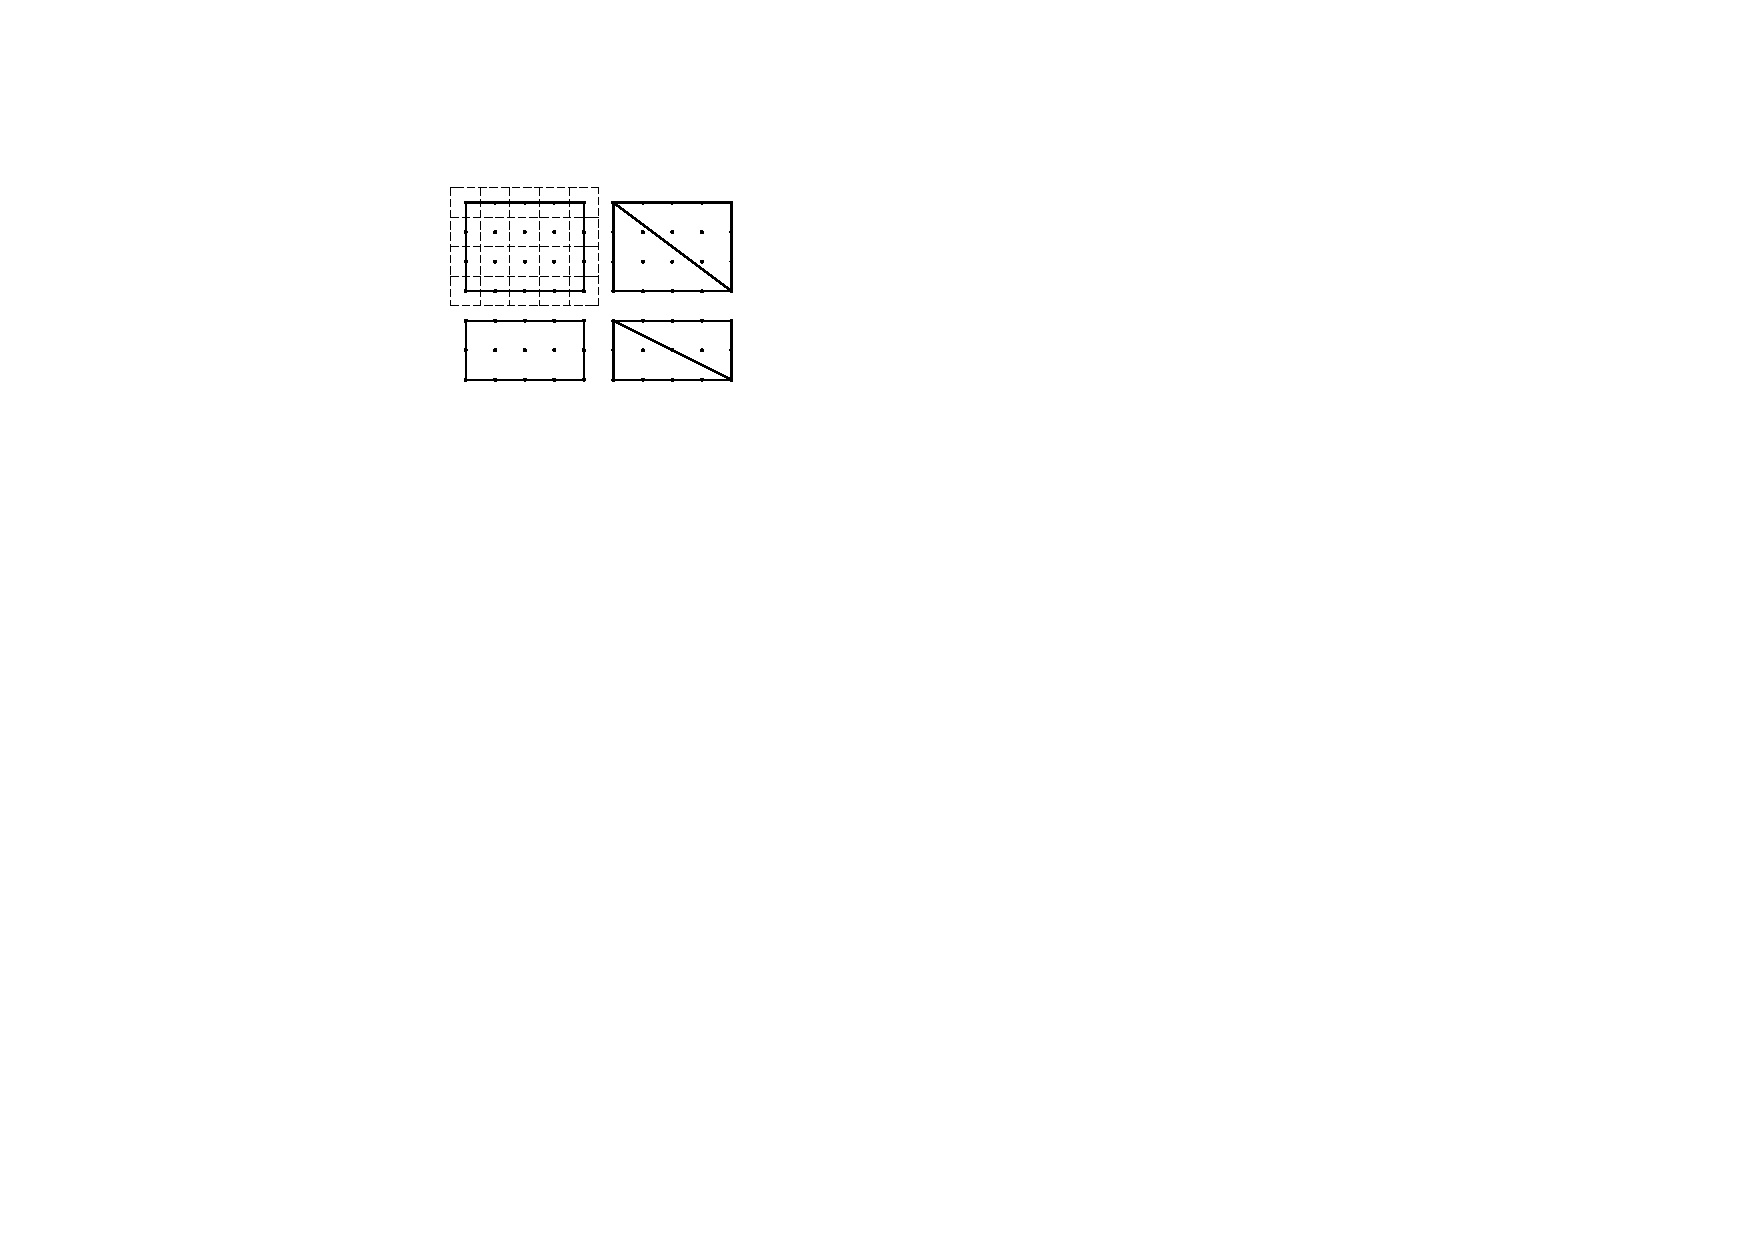
\includegraphics[width=0.7\linewidth]{PDF_Picture/格点多边形-皮克公式}
\end{figure}
矩形面积$ S=mn $,内部格点数$ N=(m-1)(n-1)=mn-(m+n)+1 $,
边界格点数$ B=2(n+m) $,
所以$ S=mn=N+\dfrac{B}{2}-1 $. 
用晶胞原子计数方法重新叙述一遍:
晶胞内部的原子有$ N $个,每个的贡献是1;
晶胞边界(不含顶点)的原子有$ B-4 $个,每个的贡献是$ \dfrac{1}{2} $;
晶胞顶点的原子有$ 4 $个,每个的贡献是$ \dfrac{1}{4} $;于是原子总数为:
$ N+(B-4)\cdot\dfrac{1}{2}+4\cdot \dfrac{1}{4}=N+\dfrac{B}{2}-1 $.\\
接下来考虑用一条对角线将上述矩形分割成两个全等的直角三角形,
除去对角线的两个端点,设对角线经过了$ d $个原始矩形的内部点,
那么,$ N_{\Delta}=\dfrac{N-d}{2} $,$ B_{\Delta}=\dfrac{B}{2}+1+d $,
直角三角形的面积
\begin{gather*}
    S_{\Delta}=\dfrac{1}{2}\left(N+\dfrac{B}{2}-1\right)
    =\dfrac{N-d}{2}+\dfrac{\frac{B}{2}+1+d}{2}-1=
    N_{\Delta}+\dfrac{B_{\Delta}}{2}-1
\end{gather*}
说明皮克公式对于直角边分别平行于$ x,y $轴的直角三角形也成立。
而其它任意形状的三角形,均可用一个两组对边分别平行于$ x,y $轴
且面积最小的格点矩形将其包围,然后减去若干个直角三角形获得。
如下图。同时,任意形状的多边形,均可拆分为若干个三角形,请读者自行分析。
\begin{figure}[H]
    \centering
    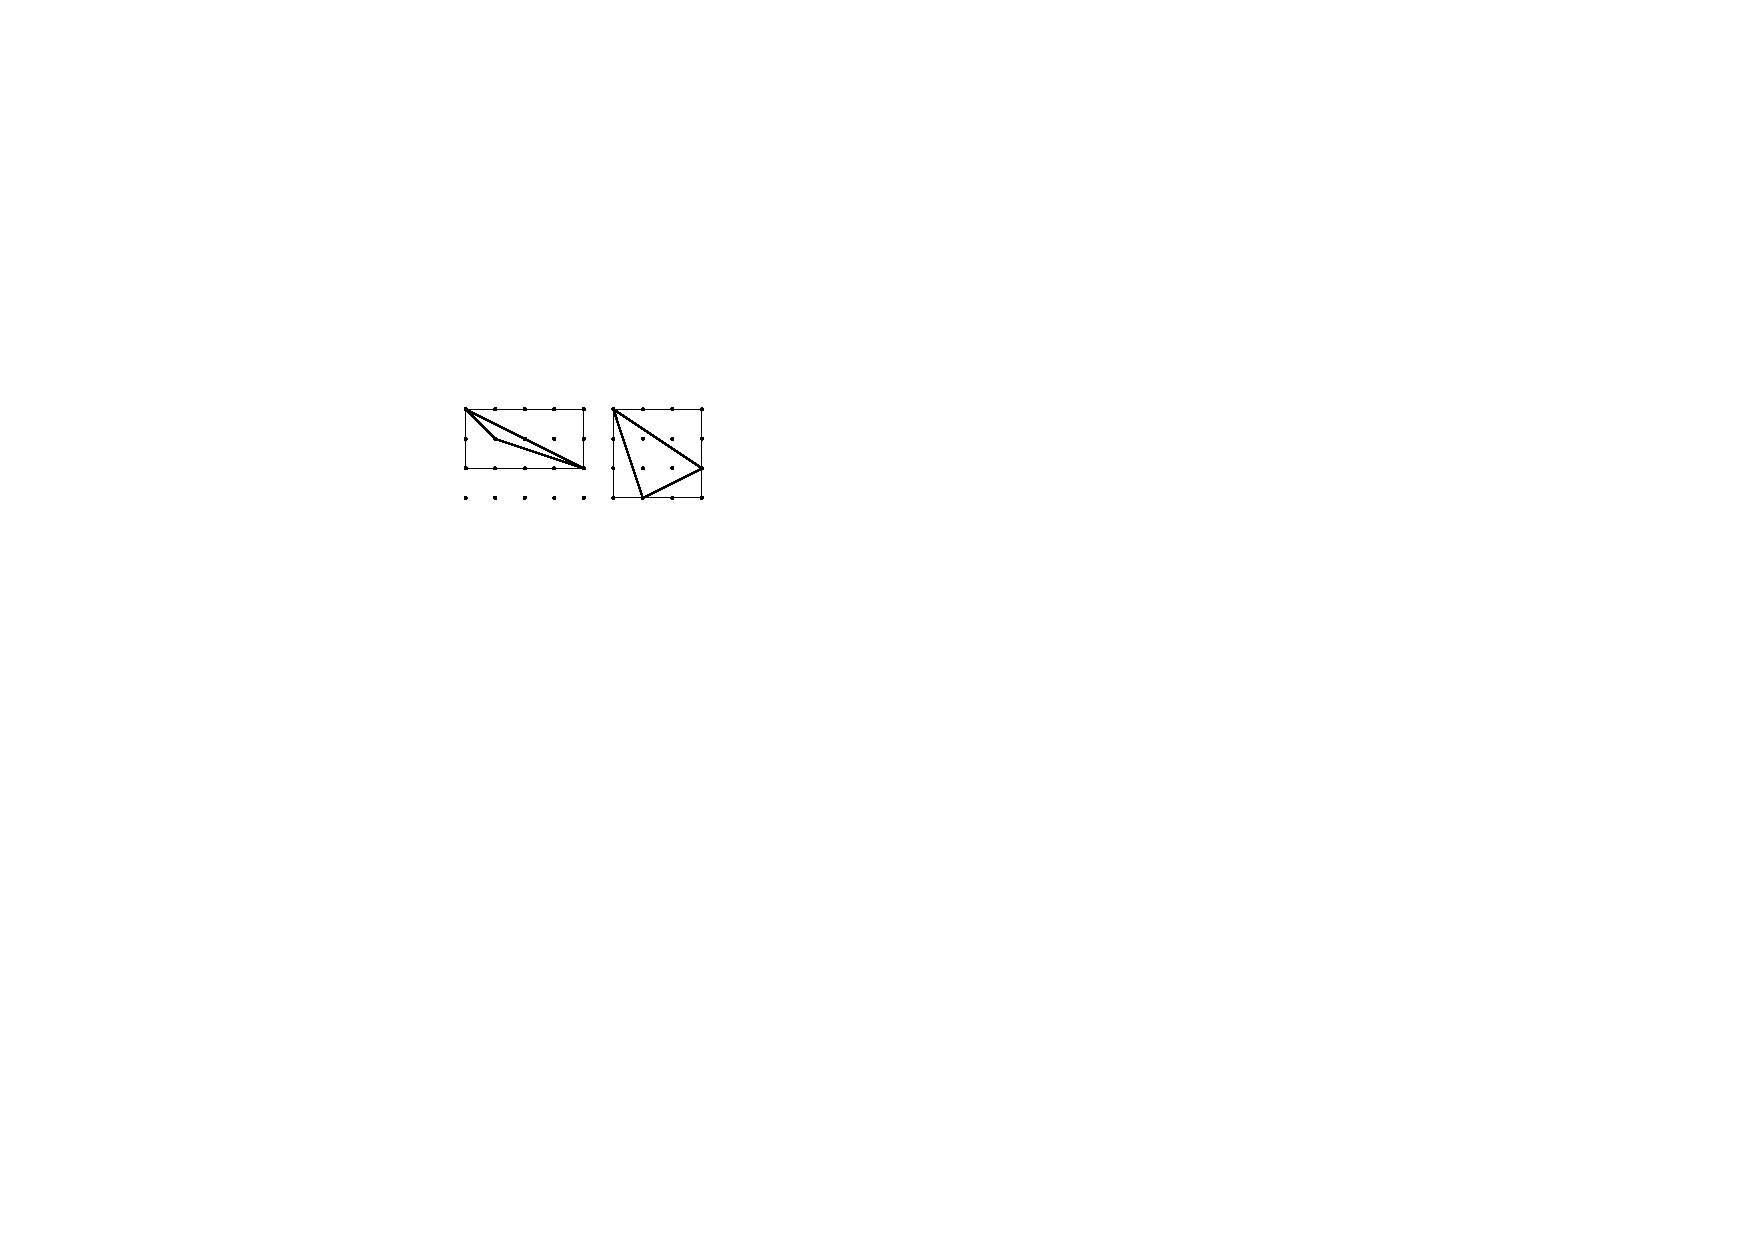
\includegraphics[width=0.65\linewidth]{PDF_Picture/任意三角形-皮克公式}
\end{figure}

\item 设多边形的顶点按顺时针(或逆时针)方向依次为
$ P_1(x_1, y_1), P_2(x_2, y_2),\cdots, P_{n}(x_{n}, y_{n}) $,
则多边形面积为
\begin{align}\label{多边形面积公式}
    S=&\ \frac{1}{2}\left|(x_1y_2+x_2y_{3}+x_{3}y_{4}+\cdots+
    x_{n-1}y_{n}+ x_{n}y_1) \right. \notag \\ 
    & \left. -(x_2y_1+x_{3}y_2+x_{4}y_{3}+\cdots
    +x_{n}y_{n-1}+x_1y_{n})\right| \\
    =&\ \frac{1}{2} \left|\left(
    \begin{vmatrix}
        {x_1} & {y_1} \\
        {x_2} & {y_2} \\
    \end{vmatrix}+
    \begin{vmatrix}
        {x_2} & {y_2} \\
        {x_3} & {y_3} \\
    \end{vmatrix}+\cdots+
    \begin{vmatrix}
        {x_{n-1}} & {y_{n-1}} \\
        {x_{n}} & {y_{n}} \\
    \end{vmatrix}  +
    \begin{vmatrix}
        {x_{n}} & {y_{n}} \\
        {x_1} & {y_1} \\
    \end{vmatrix}   \right) \right|
\end{align}
注意,对于第二个等号右侧的式子,小括号里面的两条竖线表示二阶行列式
(即$ \begin{vmatrix}
    {x_1} & {y_1} \\
    {x_2} & {y_2} \\
\end{vmatrix}=x_1y_2-x_2y_1 $),
小括号外面的两条竖线表示绝对值。这个公式的证明倒是十分简单,
以四边形为例($ n=4 $),展示两种证明方法。
\begin{figure}[H]
    \centering
    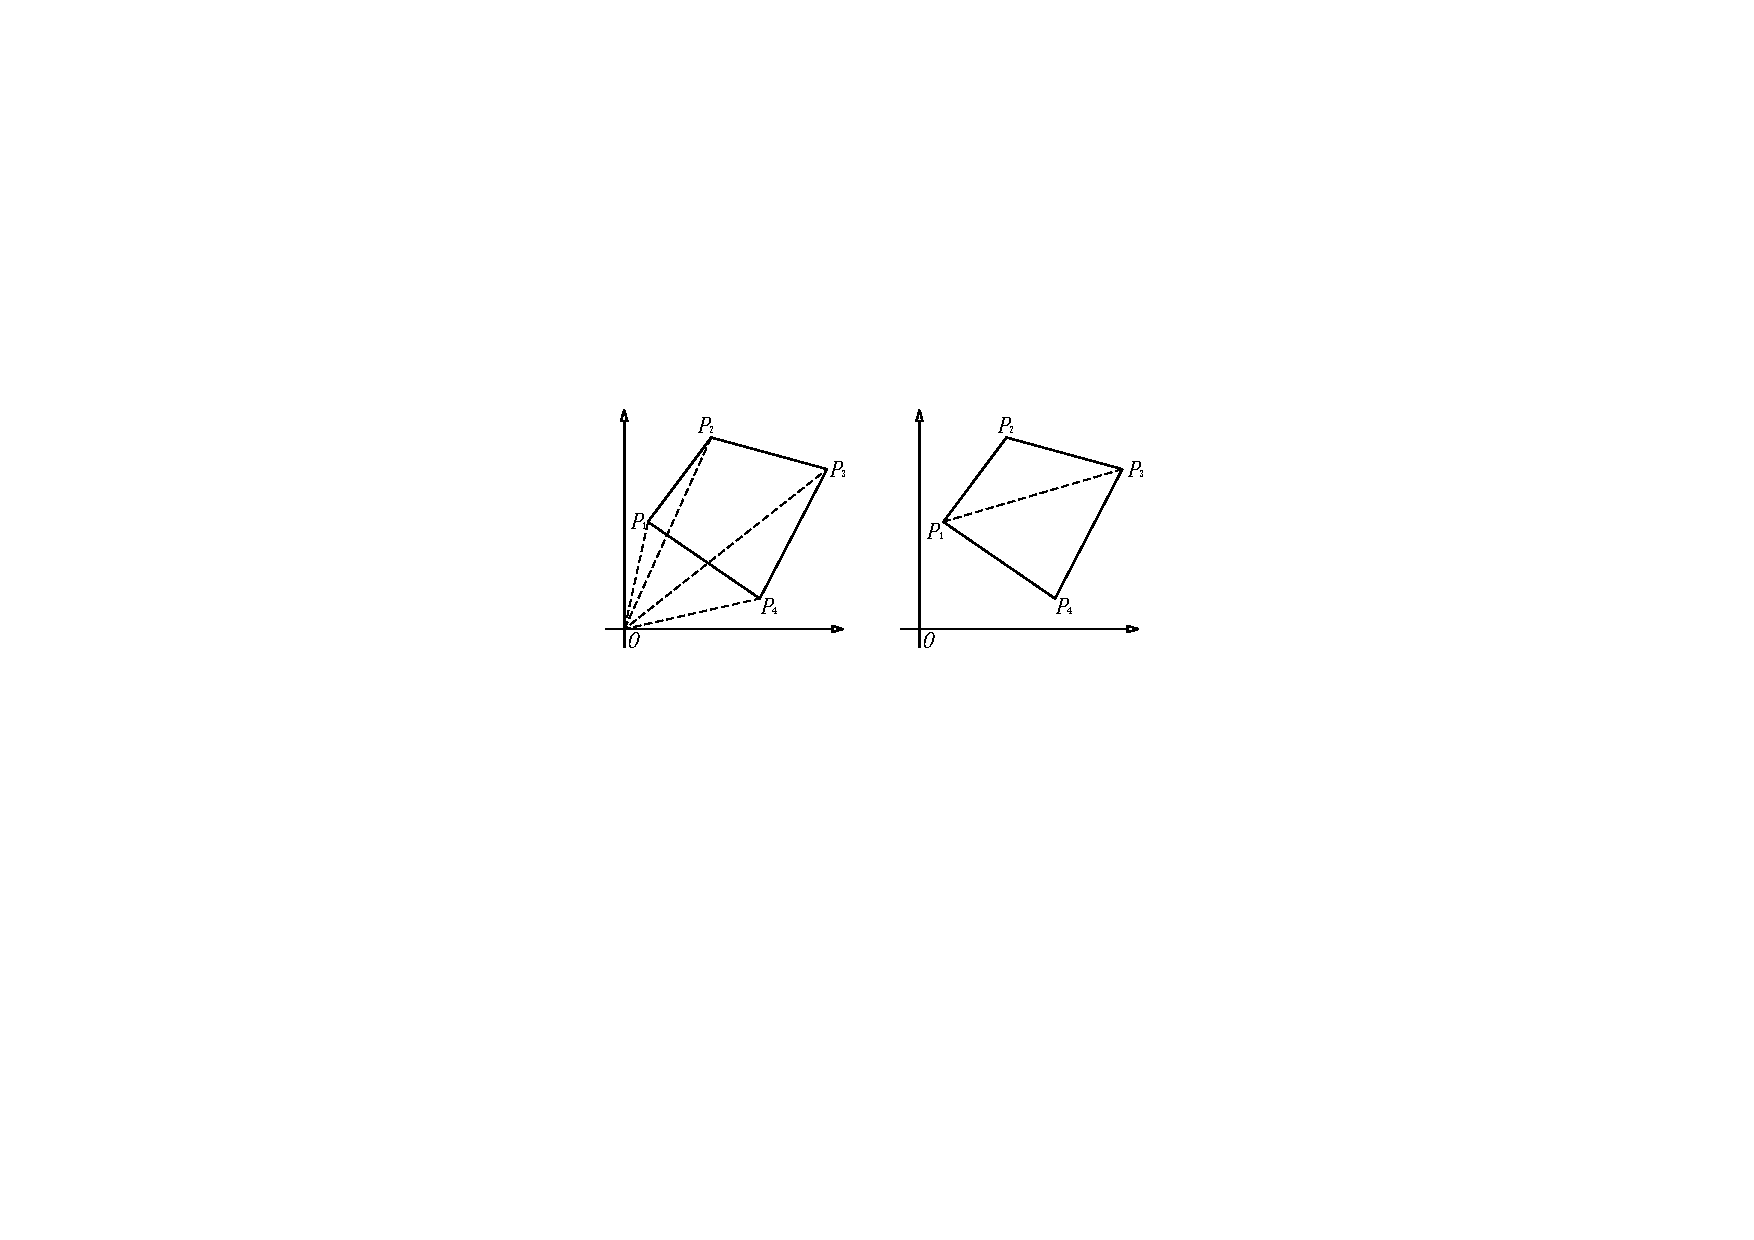
\includegraphics[width=0.6\linewidth]{PDF_Picture/多边形面积公式}
\end{figure}
方法一:如上面左图,分别连接坐标原点$ O $与所有的多边形顶点,
产生了$ \Delta OP_1P_2,\\ \Delta OP_2P_3,\ \Delta OP_3P_4,\ 
\Delta OP_4P_1 $这$ n $个三角形,注意,前$ n-1 $个三角形的顶点在书写时
都是按照顺时针的顺序,而第$ n $个三角形的顶点在书写时
是按照逆时针的顺序。假如我们约定,在利用二阶行列式计算三角形
$ \Delta OP_iP_j $的(有向)面积时,把$ \vec{OP_i} $的坐标写在行列式
的第一行,把$ \vec{OP_j} $的坐标写在行列式的第二行。
如果改变了顶点的书写顺序,就
会导致行列式的第一行与第二行交换位置,行列式的值就会反号。即
\begin{gather*}
    \begin{vmatrix}
        {x_{n}} & {y_{n}} \\
        {x_1} & {y_1} \\
    \end{vmatrix} =x_ny_1-x_1y_n=-(x_1y_n-x_ny_1)=-
    \begin{vmatrix}
        {x_1} & {y_1} \\
        {x_{n}} & {y_{n}} \\
    \end{vmatrix}
\end{gather*}
前$ n-1 $个二阶行列式,第一行的下标均小于第二行(顶点按顺时针书写),
只有最后一个行列式第一行的下标大于第二行(顶点按逆时针书写),
这就意味着最后一个行列式的符号与前$ n-1 $个不同,这正好对应了
\begin{align*}
    S_{P_1P_2P_3P_4}=&\ S_{\Delta OP_1P_2}+S_{\Delta OP_2P_3}+
    S_{\Delta OP_3P_4}-S_{\Delta OP_4P_1} \\
    =&\ \frac{1}{2} \left|\left(
    \begin{vmatrix}
        {x_1} & {y_1} \\
        {x_2} & {y_2} \\
    \end{vmatrix}+
    \begin{vmatrix}
        {x_2} & {y_2} \\
        {x_3} & {y_3} \\
    \end{vmatrix}+
    \begin{vmatrix}
        {x_3} & {y_3} \\
        {x_4} & {y_4} \\
    \end{vmatrix} -
    \begin{vmatrix}
        {x_1} & {y_1} \\
        {x_4} & {y_4} \\
    \end{vmatrix}   \right) \right| \\
    =&\ \frac{1}{2} \left|\left(
    \begin{vmatrix}
        {x_1} & {y_1} \\
        {x_2} & {y_2} \\
    \end{vmatrix}+
    \begin{vmatrix}
        {x_2} & {y_2} \\
        {x_3} & {y_3} \\
    \end{vmatrix}+
    \begin{vmatrix}
        {x_3} & {y_3} \\
        {x_4} & {y_4} \\
    \end{vmatrix} +
    \begin{vmatrix}
        {x_4} & {y_4} \\
        {x_1} & {y_1} \\
    \end{vmatrix}   \right) \right| \\
    =&\  \frac{1}{2}\left|(x_1y_2+x_2y_{3}+x_{3}y_{4}+x_4y_1)-
    (x_2y_1+x_{3}y_2+x_{4}y_{3}+x_1y_4)\right|
\end{align*}

方法二:如上面右图,从$ P_1 $点向所有不相邻的顶点作对角线,可将多边形
划分成$ n-2 $个三角形,即$ \Delta P_1P_2P_3,\ \Delta P_1P_3P_4 $,
那么
\begin{align*}
    S_{P_1P_2P_3P_4}=&\ S_{\Delta P_1P_2P_3}+S_{\Delta P_1P_3P_4}\\
    =&\ \frac{1}{2} \left|\left(
    \begin{vmatrix}
        {x_2-x_1} & {y_2-y_1} \\
        {x_3-x_1} & {y_3-y_1} \\
    \end{vmatrix}+
    \begin{vmatrix}
        {x_3-x_1} & {y_3-y_1} \\
        {x_4-x_1} & {y_4-y_1} \\
    \end{vmatrix}  \right) \right| \\
    =&\  \frac{1}{2}\left|(x_1y_2+x_2y_{3}+x_{3}y_{4}+x_4y_1)-
    (x_2y_1+x_{3}y_2+x_{4}y_{3}+x_1y_4)\right|
\end{align*}

虽然笔者在这里使用凸多边形做的演示,但这些方法对凹多边形同样适用,
请读者自行分析。

\end{itemize}

\section{例题}

\begin{enumerate}[label={【\textbf{例\thechapter.\arabic*}】},
 leftmargin=\inteval{\myenumleftmargin}pt,
 itemsep=\inteval{\myenumitempsep}pt,
 itemindent=\inteval{\myenumitemindent}pt]
\item 设$ \Delta ABC $的垂心为$ H $,且$ 3\vec{HA}+4\vec{HB}
+5\vec{HC}=\vec{0} $,求$ \cos\angle BHC $. \\
\textbf{解}\ 根据(\ref{垂心性质三个连等式})式,可设 $ \vec{HA}\cdot
\vec{HB}=\vec{HA}
\cdot\vec{HC}=\vec{HB}\cdot \vec{HC}=t<0 $,分别用
$ \vec{HB},\vec{HC} $与$ 3\vec{HA}+
4\vec{HB} +5\vec{HC}=\vec{0} $做数量积,有
\begin{gather*}
    \begin{cases}
        \vec{HB}\cdot (3\vec{HA}+4\vec{HB} +5\vec{HC})=
        3t+4|\vec{HB}|^2+5t= 0 \\
        \vec{HC}\cdot (3\vec{HA}+4\vec{HB} +5\vec{HC})=
        3t+4t+5|\vec{HC}|^2= 0 
    \end{cases} \Rightarrow \q 
    \begin{cases}
        |\vec{HB}|=\sqrt{-2t}\\
        |\vec{HC}|=\sqrt{-\dfrac{7t}{5}}
    \end{cases}
\end{gather*}
所以,
\begin{gather*}
    \cos\angle BHC=\dfrac{\vec{HB}\cdot \vec{HC}}
    {|\vec{HB}||\vec{HC}|}=\dfrac{t}{\sqrt{-2t}\sqrt{-\frac{7t}{5}}}
    =-\dfrac{\sqrt{70}}{14} 
\end{gather*}

类似地可以计算出$ \cos\angle BHA,\ \cos\angle CHA $,实际上就知道了
$ \cos\angle ABC,\cos\angle BCA,\\ \cos\angle CAB $,
三角形的形状也能确定了。另外,条件$ 3\vec{HA}+4\vec{HB}
+5\vec{HC}=\vec{0} $还可变形成$ 3\vec{HA}+4(\vec{HA}+\vec{AB})
+5(\vec{HA}+\vec{AC})=\vec{0} $,即
$ \vec{AH}=\dfrac{1}{3}\vec{AB}+\dfrac{5}{12}\vec{AC}$.

\item 已知在$ \Delta ABC $中,$ M $是$ BC $中点,$ AM=3,\ BC=10 $,
求$ \vec{AB}\cdot \vec{AC} $的值。\\
\textbf{方法一}\ 由极化恒等式(\ref{极化恒等式}),$ \vec{AB}\cdot 
\vec{AC}=\dfrac{1}{4}[(\vec{AB}+\vec{AC})^2-
(\vec{AB}-\vec{AC})^2]=\dfrac{1}{4}[(2\vec{AM})^2-
(\vec{CB})^2]=(\vec{AM})^2-(\vec{MB})^2=9-25=-16 $. \\
\textbf{方法二}\ 既然$ \vec{AB}\cdot \vec{AC} $的值与三角形形状无关,
不妨将三角形取为特殊形状,比如令$ |AB|=|AC|=\sqrt{3^2+5^2}=\sqrt{34} $,
$ \cos\angle BAC=2\cos^2\angle MAC-1=2\cdot \dfrac{9}{34}-1=-\dfrac{16}{34} $,
$ \vec{AB}\cdot \vec{AC}=\sqrt{34}\cdot \sqrt{34}\cdot
\Big(-\dfrac{16}{34}\Big)=-16 $.

\item 在下图所示的正方形、正六边形和圆形边界上有一点$ P $,
求$ \vec{PA} \cdot \vec{PB} $的范围。
\begin{figure}[h]
    \centering
    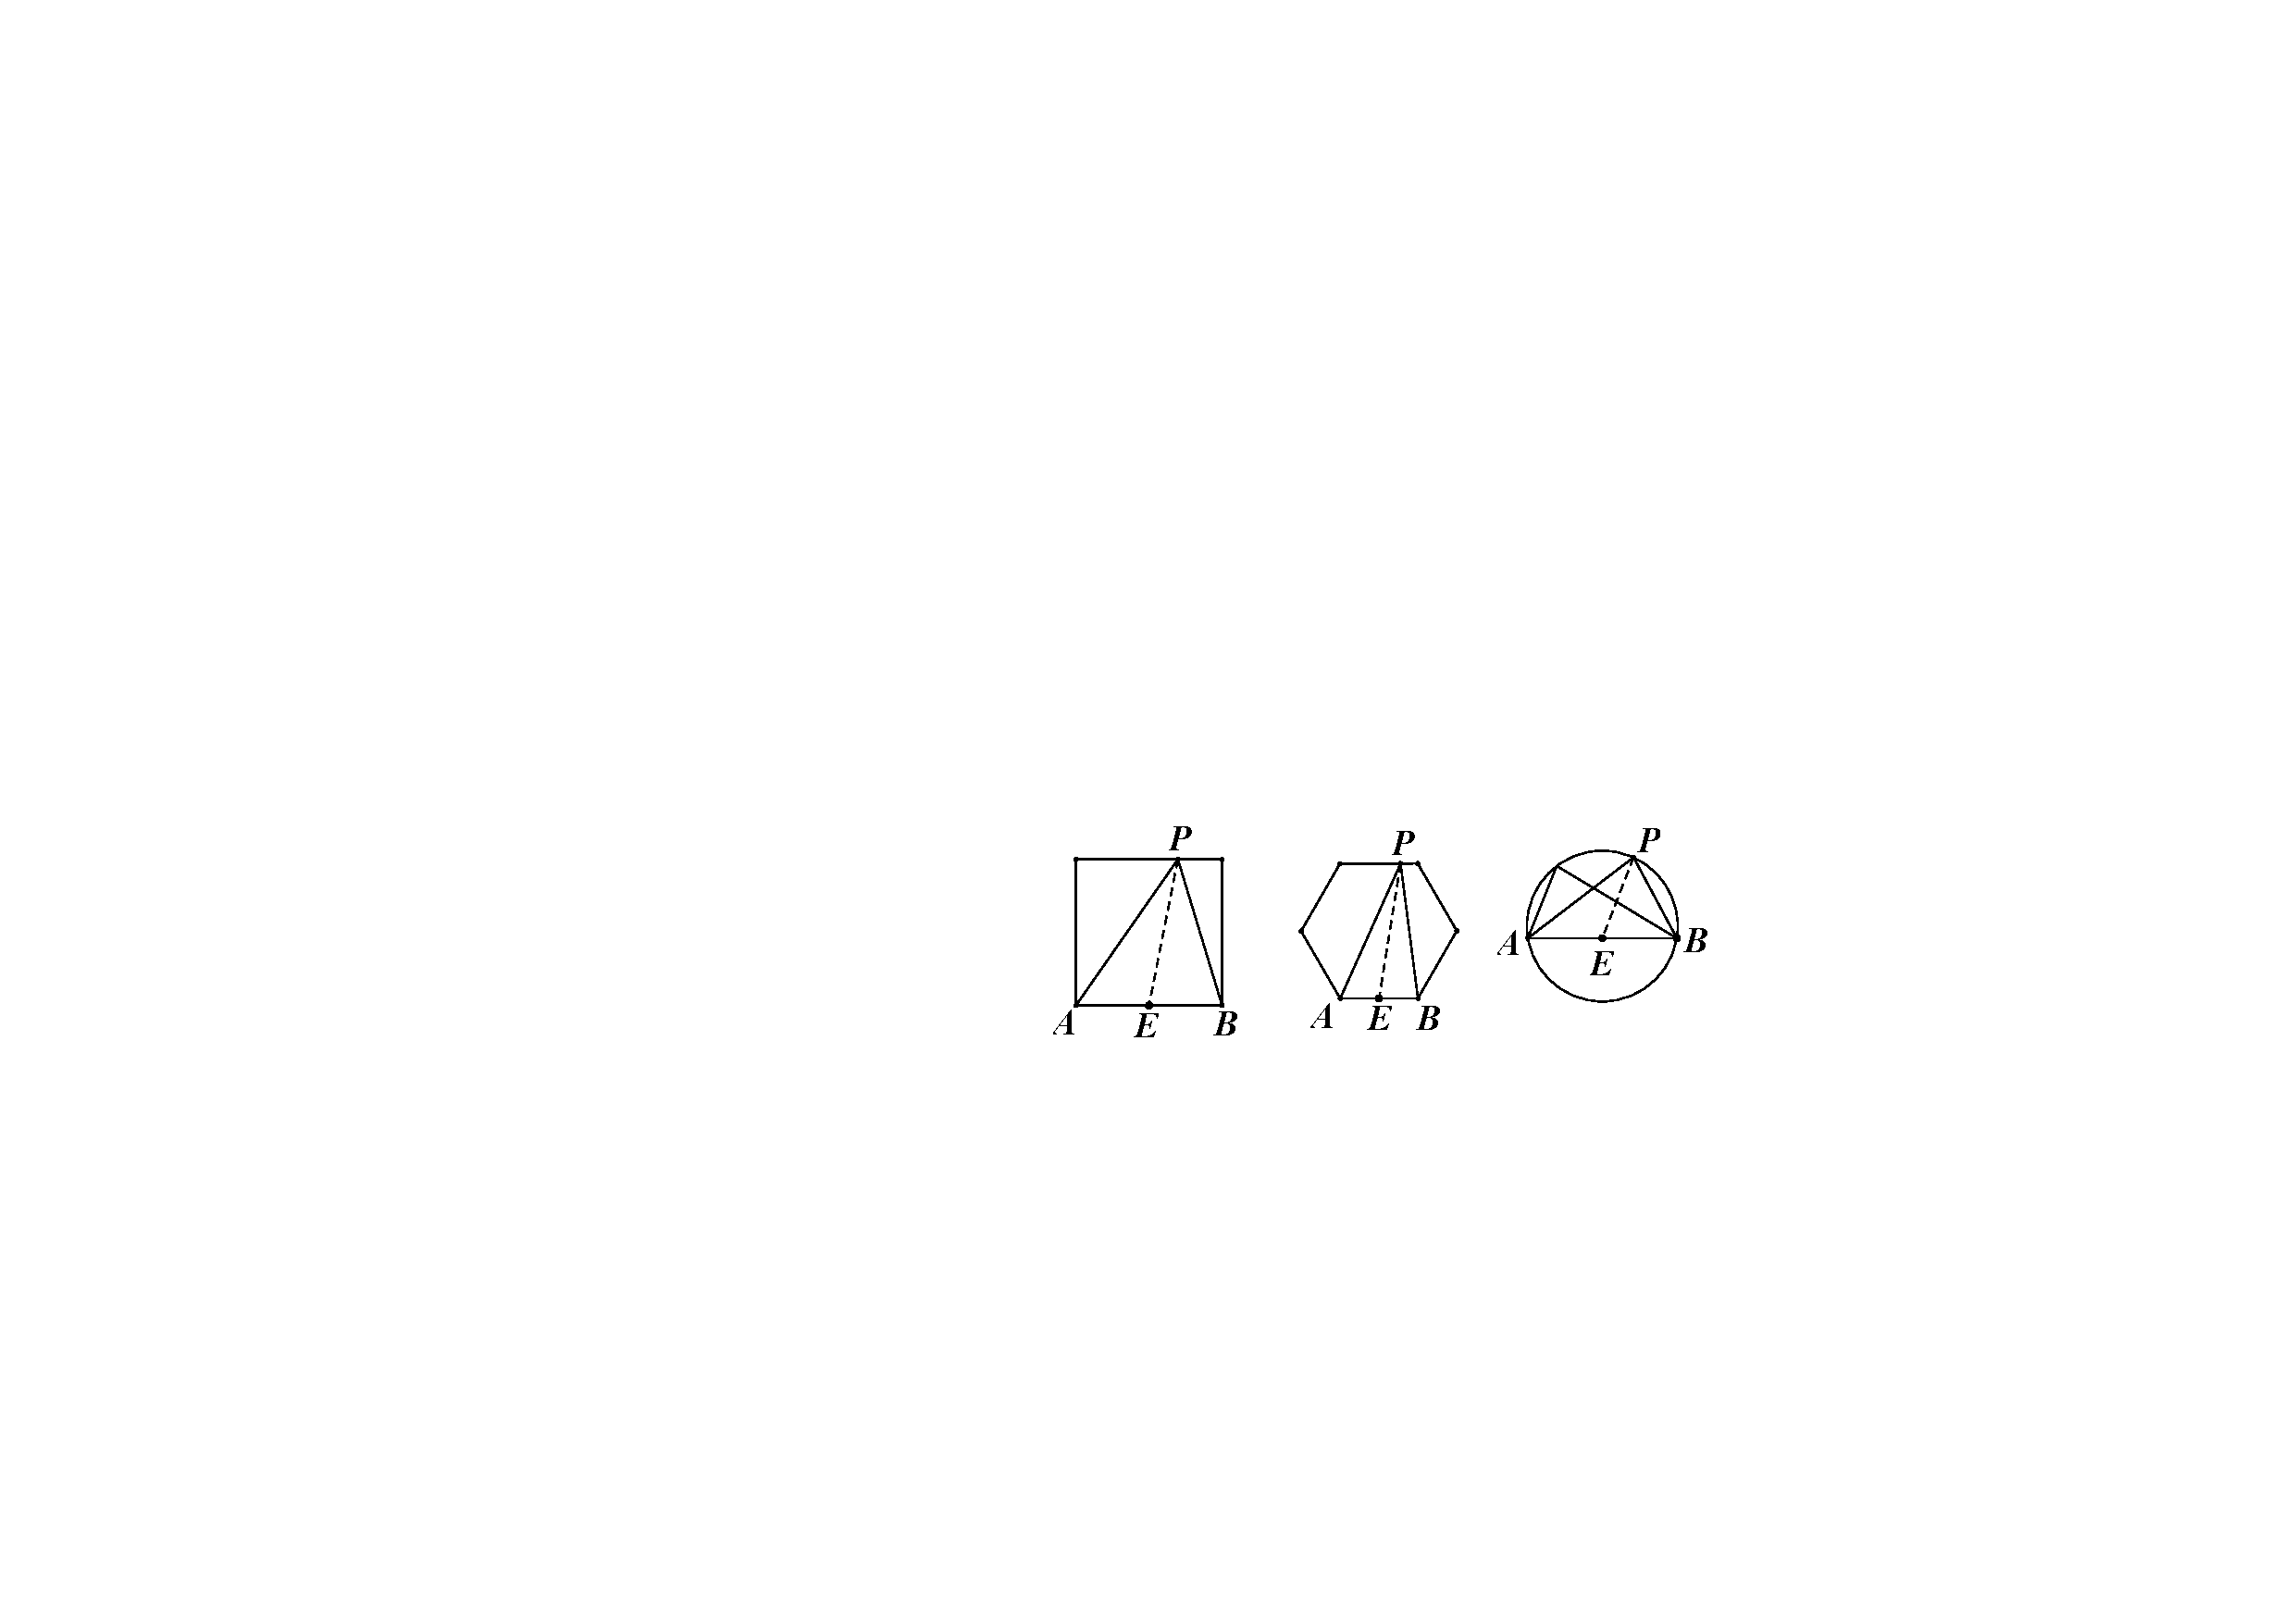
\includegraphics[width=0.6\linewidth]{向量点乘最值问题}
\end{figure} \\
\textbf{分析}\ 取$ AB $的中点$ E $,则$ \vec{PA}\cdot\vec{PB}
= \left(\vec{PE}+\vec{EA}\right)\cdot \left(
\vec{PE}-\vec{EA}\right) = \vec{PE}^2-
\vec{EA}^2 $,问题就转化成了求$ |\vec{PE}| $的范围。

另一类问题是$ \vec{PA}\cdot\vec{PB} $为定值
$ L $,求$ P $点的轨迹。只要$ L>-|\vec{EA}|^2 $,$ P $点的轨迹就是以
$ E $点为圆心,以$ \sqrt{|\vec{EA}|^2+L} $为半径的圆。

\item 在$ \Delta ABC $中,$ A=\dfrac{\pi}{3},\ AB=2 $,求
$ \vec{CA}\cdot\vec{CB} $的取值范围。\\
\textbf{解}\ 
$ \vec{CA}\cdot\vec{CB}=\vec{CA}\cdot(
\vec{CA}+\vec{AB})=\vec{CA}^2+
\vec{CA}\cdot\vec{AB}
=|\vec{CA}|^2-|\vec{CA}|\geq -\dfrac{1}{4} $. 

\item $ \Delta ABC $的面积为3,且有$ c=3b $,求$ a $的最小值。\\
\textbf{解}\ $ S_{\Delta ABC}=\dfrac{1}{2}bc\sin A=3,\ b^2=\dfrac{2}{\sin A} $,
$ a^2=b^2+c^2-2bc\cos A=10b^2-6b^2\cos A=\dfrac{4(5-3\cos A)}{\sin A} $,
令$ k=\dfrac{5-3\cos A}{\sin A}>0 $,则$ k\sin A+3\cos A=\sqrt{k^2+9}\sin(A+\varphi)=5 
\Rightarrow \sqrt{k^2+9}\geq 5, k\geq 4 $,所以$ a=2\sqrt{k}\geq 4 $. 

\item 在$ \Delta ABC $中,$ AB=4,\ AC=\sqrt{3}BC $,
求$ \Delta ABC $面积的最大值。\\
\textbf{方法一}\ 以$ AB $所在直线为$ x $轴,$ AB $中点为原点,建立直角坐标系,设
$ A(-2,0),B(2,0),\\ C(x,y) $,那么$ (x+2)^2+y^2=3[(x-2)^2+y^2] \Rightarrow
(x-4)^2+y^2=12 $,说明$ C $点轨迹是一个圆(名为“阿波罗尼奥斯圆”),$ |y|\leq 
2\sqrt{3} $,面积最大值为$ 4\times 2\sqrt{3} \times \dfrac{1}{2}=4\sqrt{3} $. \\
\textbf{方法二}\ $ AC=\sqrt{3}BC=\sqrt{3}a $,
\begin{gather*}
    S=\dfrac{1}{2}\cdot 4 a\sin B=2a\sqrt{1-\cos^2B}=2a\sqrt{1-\left(
        \dfrac{16+a^2-3a^2}{2\cdot4\cdot a}\right)^2} \\
    =\dfrac{1}{2}\sqrt{-(a^2-16)^2+192}\leq 4\sqrt{3}
\end{gather*}

\item 在$ \Delta ABC $中,$ C=\dfrac{2\pi}{3},\ c^2=7b^2,\ S_{\Delta ABC}=
2\sqrt{3} $,求$ b $. \\
\textbf{方法一}\ $ 7b^2=c^2=a^2+b^2-2ab\cos C \Rightarrow a^2+ab-6b^2=0,\ (a+3b)
(a-2b)=0\Rightarrow a=2b,\ S_{\Delta ABC}=\dfrac{1}{2}ab\sin C=\dfrac{1}{2}(2b)b\dfrac{\sqrt{3}}{2}=2\sqrt{3},\ b=2  $. \\
\textbf{方法二}\ $ \sin C=\dfrac{\sqrt{3}}{2},\ \cos C=-\dfrac{1}{2},\ \sin B=
\dfrac{1}{\sqrt{7}}\sin C=\dfrac{\sqrt{21}}{14},\ \cos B=\dfrac{5\sqrt{7}}{14},
\ \sin A=\sin(B+C)=\dfrac{\sqrt{21}}{7},\ \ S_{\Delta ABC}=\dfrac{1}{2}bc\sin A=
\dfrac{1}{2}b(\sqrt{7}b)\dfrac{\sqrt{21}}{7}=2\sqrt{3},\ b=2 $. 

\item (2017 高考全国卷)如下图,在矩形$ ABCD $中,$ AB=1,\ AD=2 $,
动点$ P $在以点$ C $为圆心且与$ BD $相切的圆上运动,若$ \vec{AP}=
\lambda\vec{AB}+\mu\vec{AD} $,
求$ \lambda+\mu $的最大值。 
\begin{figure}[H]
    \centering
    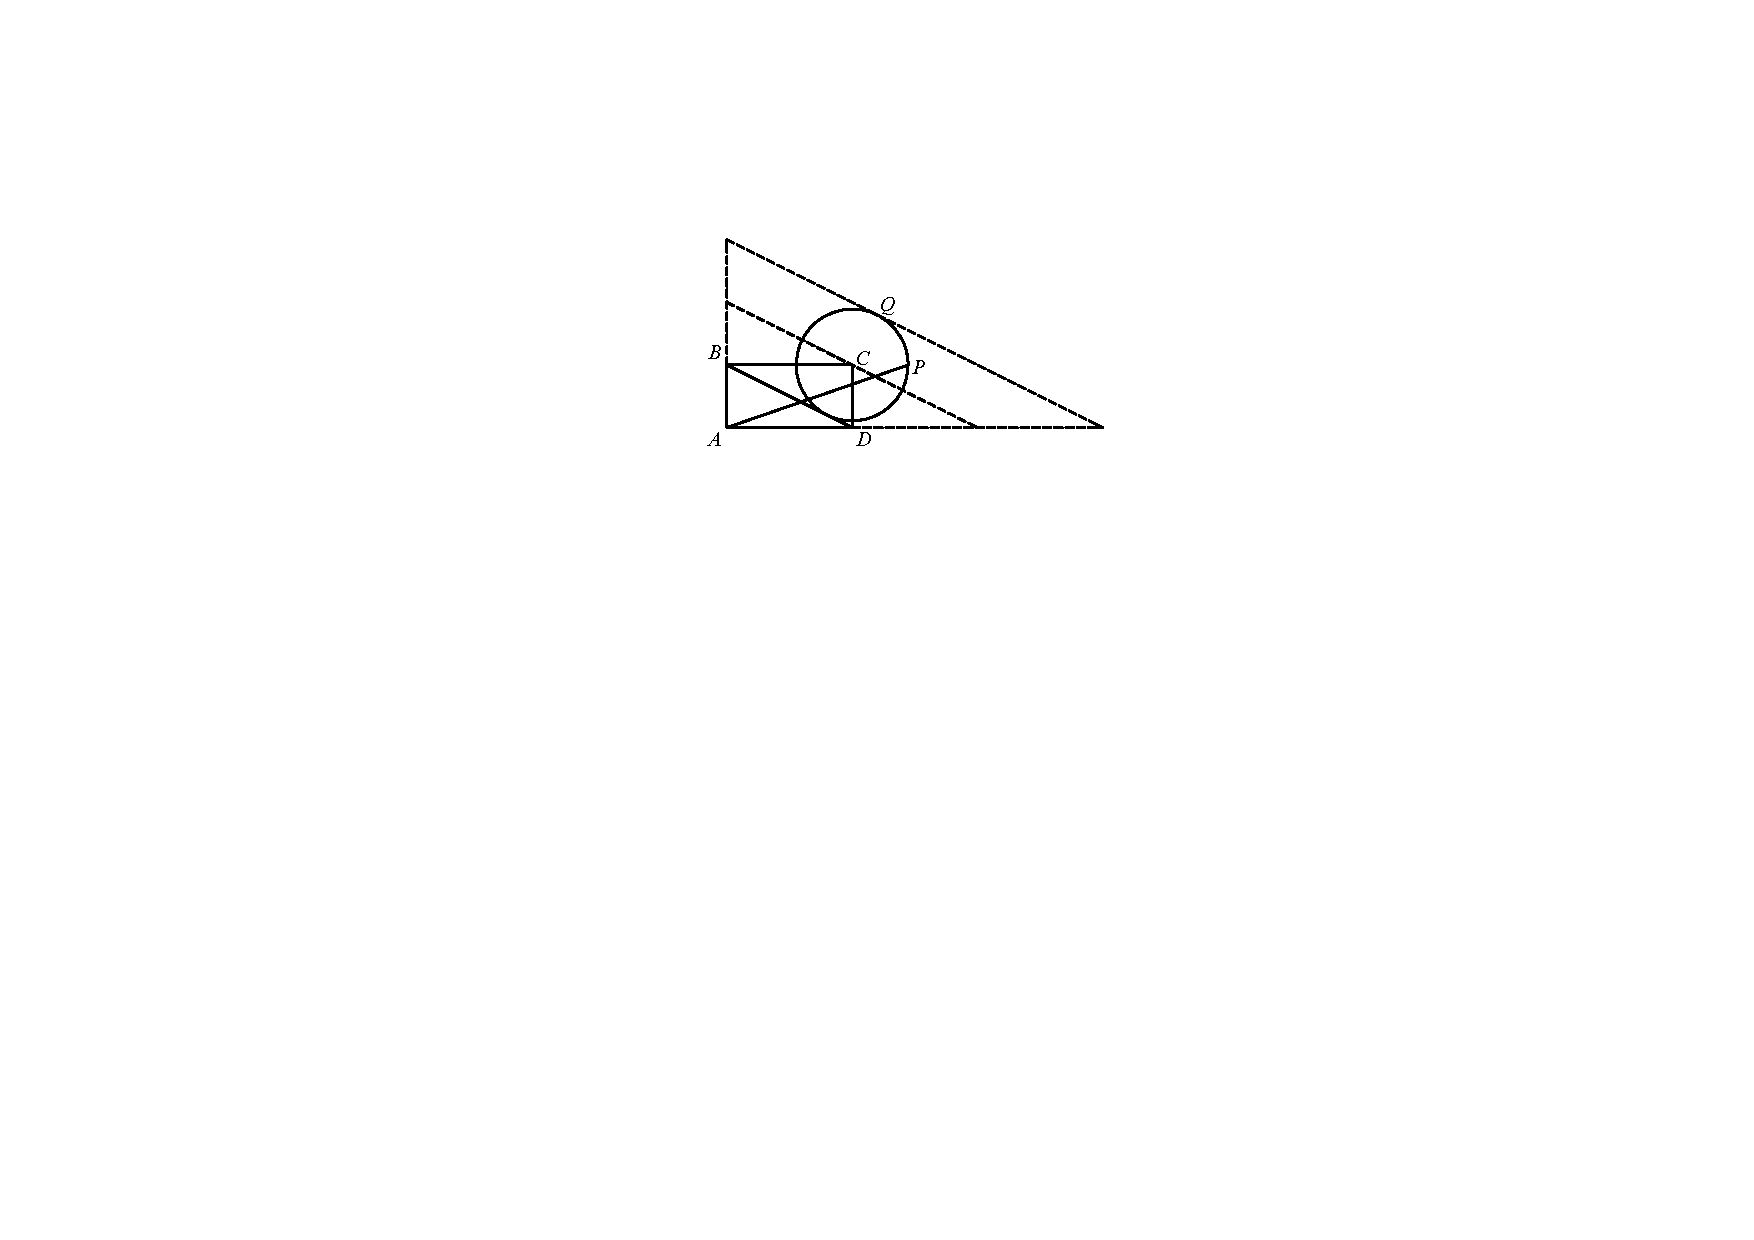
\includegraphics[width=0.35\linewidth]{向量等和线问题(带辅助线)}
\end{figure} 
\noindent\textbf{解}\ 选定一条与$ BD $平行的直线$ l $,当$ P $点在$ l $上运动时,
$ \lambda+\mu $为定值。作一条与$ BD $平行且与$ \odot C $
相切的直线,切点为$ Q $,当$ P $运动到$ Q $点时,$ \lambda+\mu $取得最大值。
根据相似三角形,最大值为3. 

\item 已知向量$ \vec{a},\vec{b} $满足
$ |\vec{a}|=1,|\vec{b}|=2$,
求$ |\vec{a}+\vec{b}|+|\vec{a}-
\vec{b}| $的最小值和最大值。\\
\textbf{解}\ 
\begin{gather*}
    \sqrt{a^2+b^2+2ab\cos\theta}+\sqrt{a^2+b^2-2ab\cos\theta}=
    \sqrt{5+4\cos\theta}+\sqrt{5-4\cos\theta}=\\
    \sqrt{\left(\sqrt{5+4\cos\theta}+\sqrt{5-4\cos\theta} 
        \right)^2}=\sqrt{10+2\sqrt{25-16\cos^2\theta}}
\end{gather*}
最小值是4,此时$ \vec{a},\vec{b} $反向;
最大值是$ 2\sqrt{5} $,此时$ \vec{a},\vec{b} $同向。
还可以求导,或者使用柯西不等式求最大值。

\item 设$ x>0,y>0 $,向量$ \vec{a}=(1-x,4),\vec{b}=
(x,-y) $,求$ \vec{a}//\vec{b} $,则$ x+y $的最小值。\\
\textbf{解}\ $ 4x+(1-x)y=0,\ \dfrac{1}{x}+\dfrac{4}{y}=1 $. \\
\textbf{方法一}\ 消元:
$ x=\dfrac{y}{y-4},x+y=\dfrac{y}{y-4}+y=(y-4)+\dfrac{4}{y-4}+5\geq 9 $. \\
\textbf{方法二}\ 基本不等式:
$ x+y=(x+y)(\dfrac{1}{x}+\dfrac{4}{y})=5+\dfrac{y}{x}+\dfrac{4x}{y}
\geq 5+ 2\sqrt{\dfrac{y}{x}\cdot \dfrac{4x}{y}}=9 $. \\
\textbf{方法三}\ 柯西不等式:$ x+y=(x+y)(\dfrac{1}{x}+\dfrac{4}{y})
\geq \left( \sqrt{x\cdot \dfrac{1}{x}}+
\sqrt{y\cdot \dfrac{4}{y}}\right) ^2=3^2=9 $. 

\item 在平面四边形$ ABCD $中,已知$ \Delta ABC $的面积是$ \Delta ADC $
的面积的3倍,若存在正实数$ x,y $使得$ \vec{AC}=\left(\dfrac{1}{x}-3
\right)\vec{AB}+\left(1-\dfrac{1}{y} 
\right)\vec{AD} $成立,求$ x+y $的最小值。\\
\textbf{解}\ 对于$ \Delta ABC $和$ \Delta ADC $,如果都以对角线$ AC $为底边,
那么两个三角形的高的比值是3,再根据相似三角形,
$ BD $被$ AC $分成3:1两段。$ 3\left(\dfrac{1}{x}-3 \right)=\left(1-
\dfrac{1}{y} \right) $,$ \dfrac{3}{x}+\dfrac{1}{y}=10 $,
$ x+y=(x+y)\cdot\dfrac{1}{10}\Big(\dfrac{3}{x}+\dfrac{1}{y}\Big)=
\dfrac{1}{10}\Big(3+1+\dfrac{3y}{x}+\dfrac{x}{y}\Big)
\geq\dfrac{2+\sqrt{3}}{5} $. 

\item 设向量$ \vec{a},\vec{b},\vec{c} $
满足$ |\vec{a}|=|\vec{b}|=1,\vec{a}\cdot
\vec{b}=-\dfrac{1}{2},\langle\vec{a}-\vec{c},
\vec{b}-\vec{c}\rangle=\dfrac{\pi}{3} $,
则$ |\vec{c}| $的最大值是多少?
\begin{figure}[h]
    \centering
    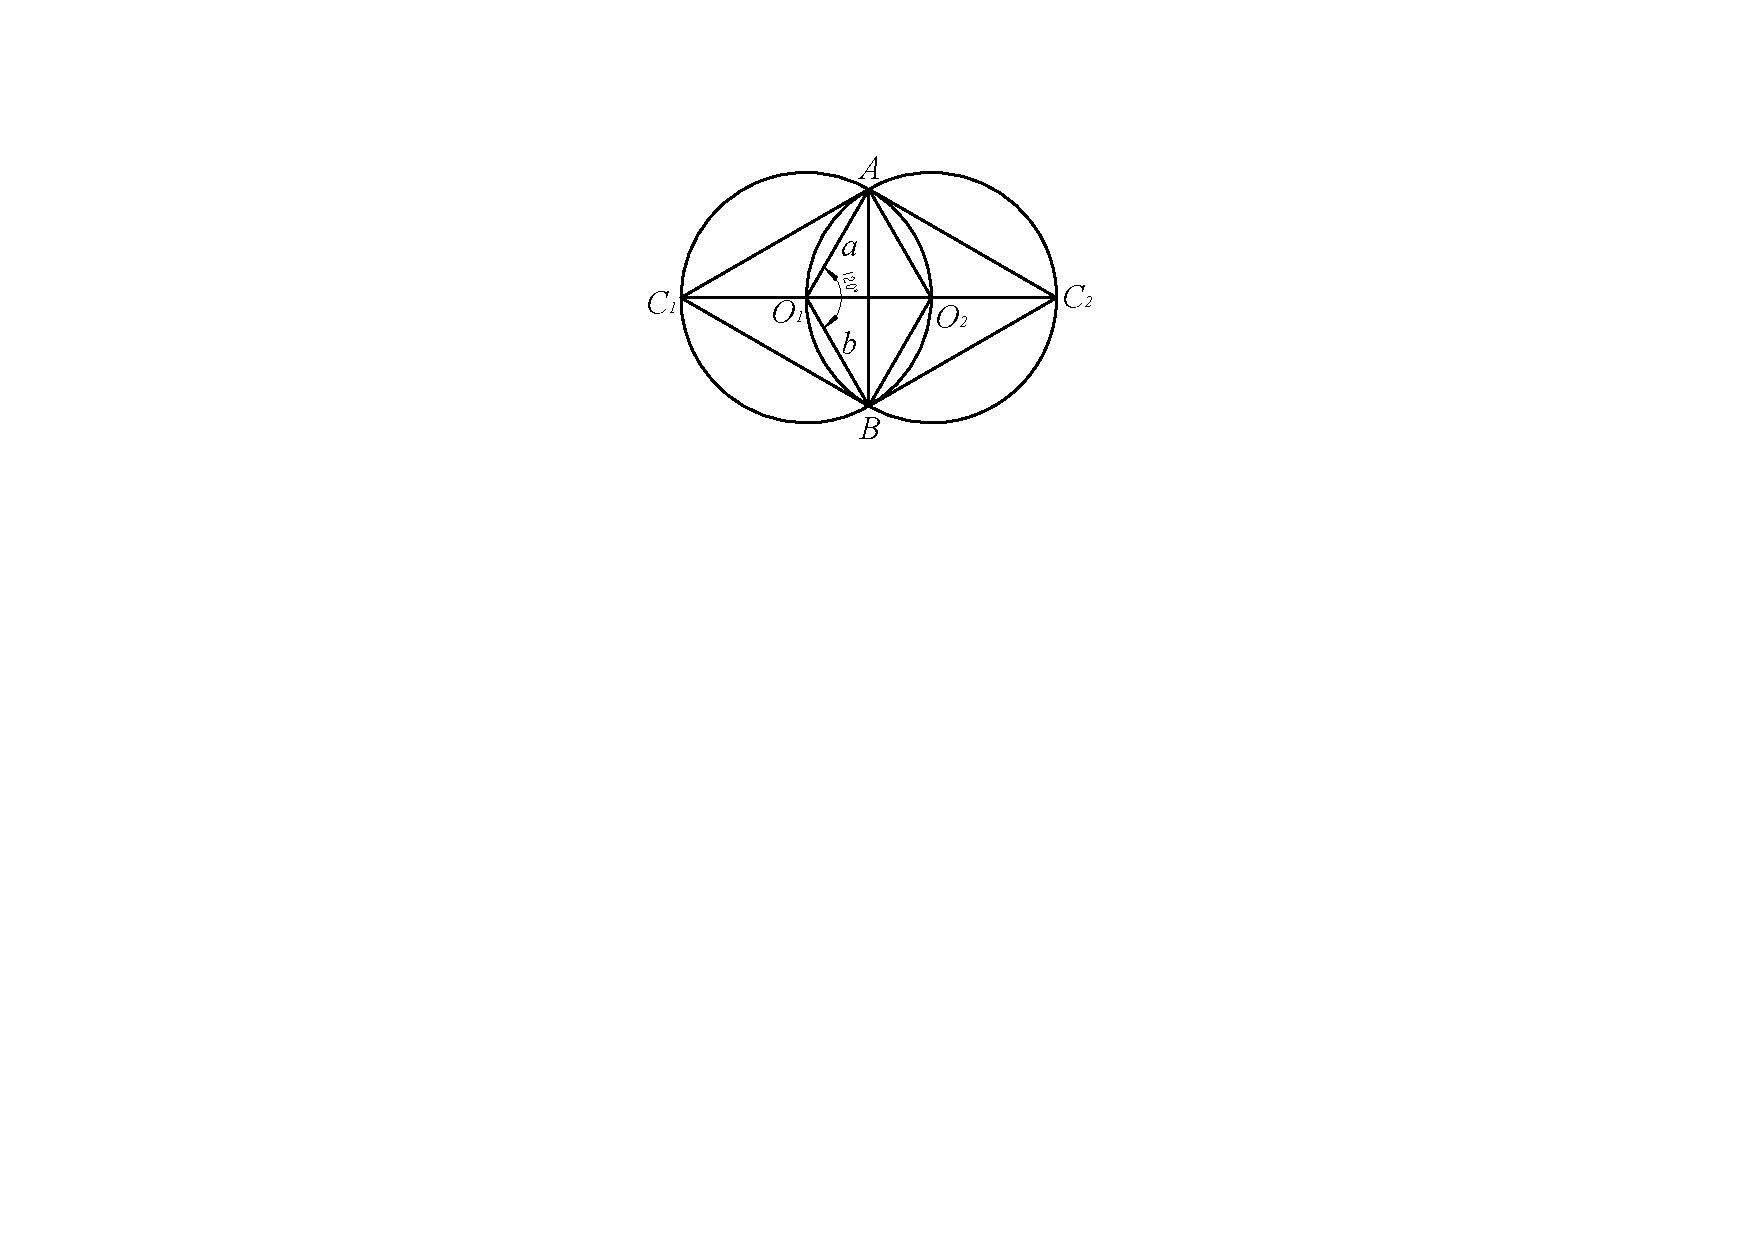
\includegraphics[width=0.4\linewidth]{向量-四点共圆题}
\end{figure} \\
\textbf{解}\ $ \vec{O_1A}=\vec{a},\ \vec{O_1B}=
\vec{b},\angle AOB=120^\circ $,$ \vec{c} $的终点可能在$ \odot 
O_1 $或$ \odot O_2 $上,$ |\vec{c}| $最大是$ |O_1C_2|=2 $ .

\item 在$ \Delta ABC $中,$ \vec{AB}=(\sqrt{3}\cos x,\cos x),
\vec{AC}=(\cos x,\sin x) $,则$ \Delta ABC $面积的最大值是多少?\\
\textbf{解}\ 根据(\ref{三角形面积公式x1y2-x2y1})式,$ S_{\Delta ABC}=\dfrac{1}{2}
\left|\sqrt{3}\cos x\sin x-\cos^2 x\right|=\dfrac{1}{2}\left|\dfrac{\sqrt{3}}{2}
\sin 2x-\dfrac{1}{2}\cos 2x-\dfrac{1}{2}\right|
=\dfrac{1}{2}\left|\sin\Big(2x-\dfrac{\pi}{6}\Big)-\dfrac{1}{2}\right|
\leq \dfrac{3}{4} $. 

\item 已知点$ M,N $在以$ AB $为直径的圆上,若$ AB=5,AM=3,BN=2 $ ,
求$ \vec{AB}\cdot\vec{MN} $. 
\begin{figure}[H]
    \centering
    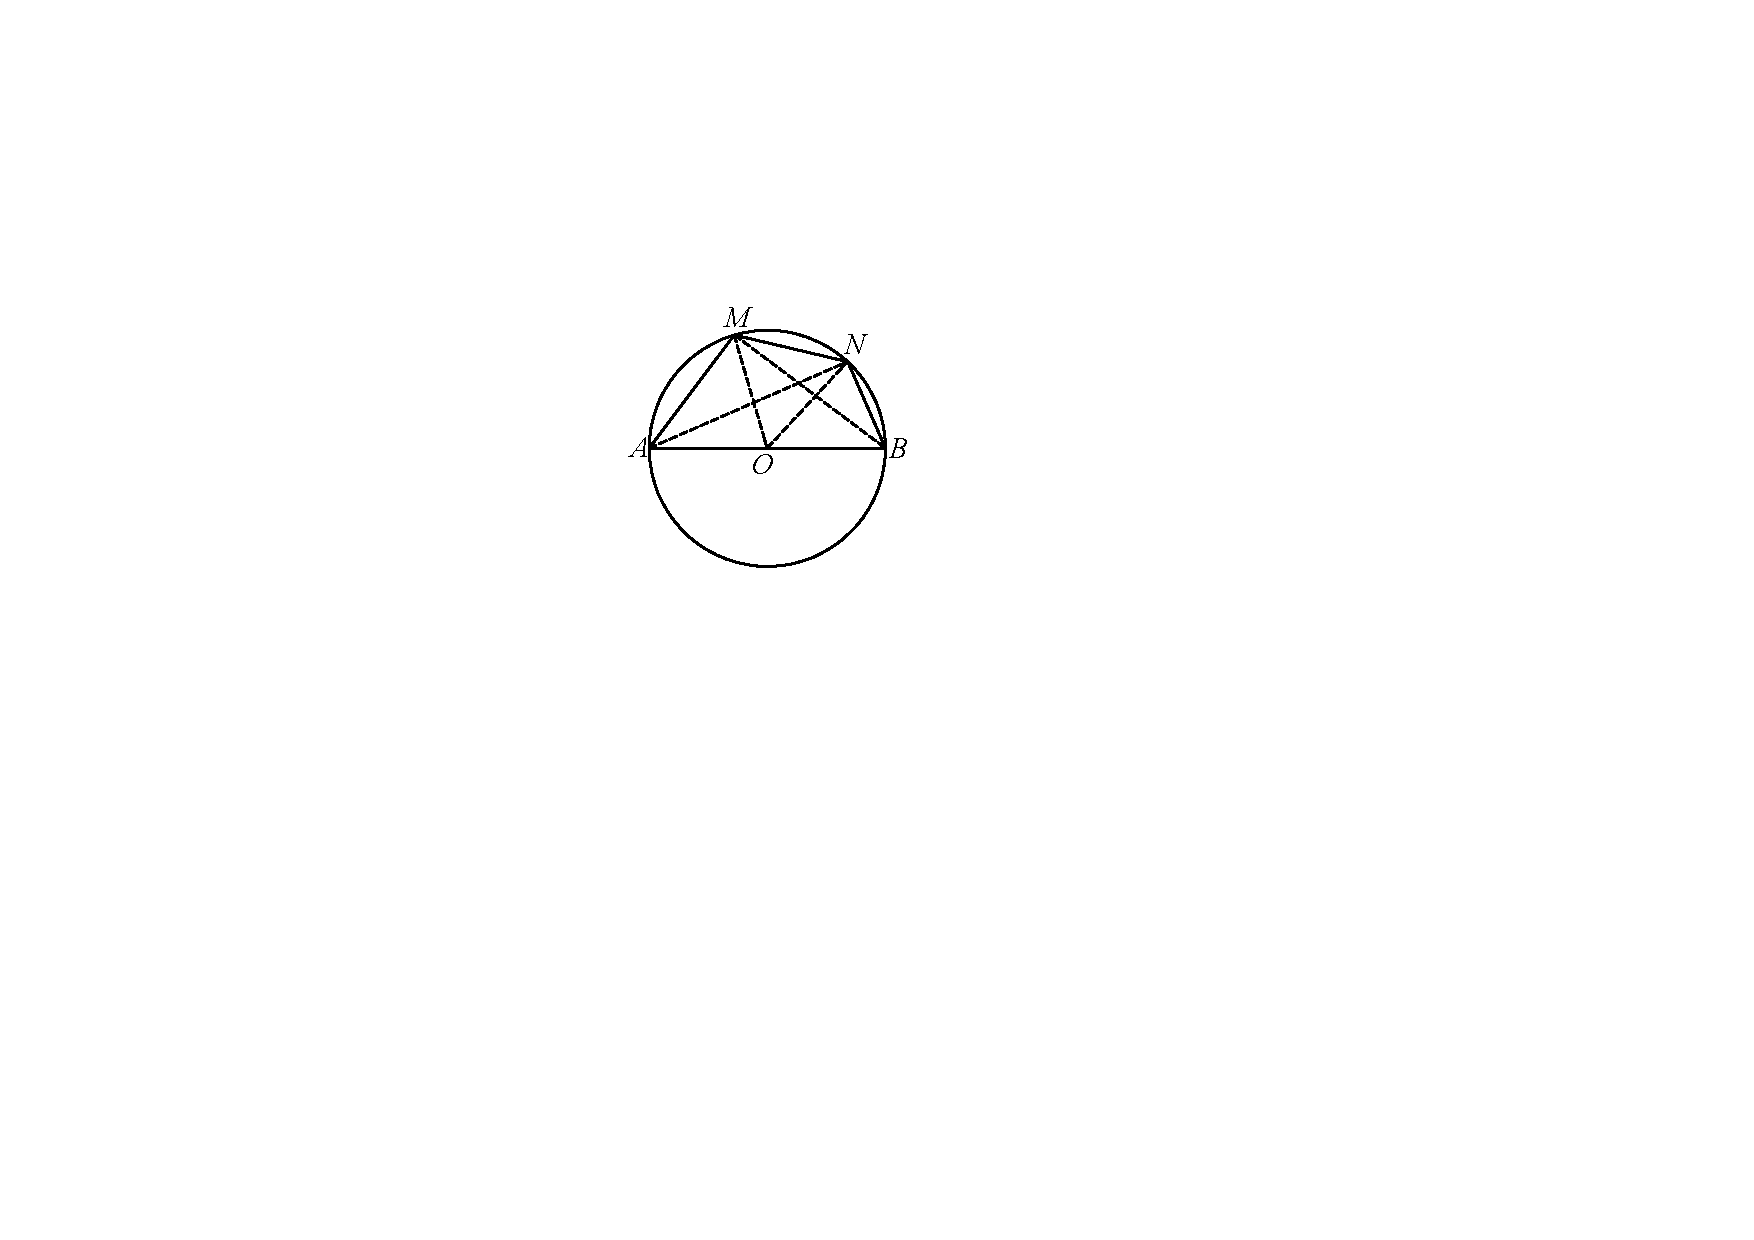
\includegraphics[width=0.3\linewidth]{向量题圆AB=5}
\end{figure}
\noindent\textbf{方法一}\ $ \vec{AB}\cdot\vec{MN}=\vec{AB}
\cdot(\vec{AN}-\vec{AM})=\vec{AB}\cdot
\vec{AN}-\vec{AB}\cdot\vec{AM}=
|AN|^2-|AM|^2=(|AB|^2-|BN|^2)-|AM|^2=25-4-9=12 $. \\
\textbf{方法二}\ $ \cos\angle AOM=\dfrac{7}{25},\ \cos\angle BON=\dfrac{17}{25} $,
以$ O $为原点,$ OB $为$ x $轴正半轴建立坐标系,则
$ M\left(-\dfrac{5}{2}\cdot\dfrac{7}{25},y_M\right) $,
$ N\left(\dfrac{5}{2}\cdot\dfrac{17}{25},y_N\right) $,
$ \vec{MN}=\left(\dfrac{12}{5},y_N-y_M\right) $,$ \vec{AB}=(5,0) $,
$ \vec{AB}\cdot\vec{MN}=5\cdot\dfrac{12}{5}=12 $. \\
\textbf{注}\ 不论$ M,N $两点分布在直径$ AB $同侧还是两侧,最终结果是一样的。

\item (2022,新高考I卷)已知$ \Delta ABC $满足$ \dfrac{\cos A}{1+\sin A}=
\dfrac{\sin 2B}{1+\cos 2B} $. \\
(1)若$ C=\dfrac{2\pi}{3} $,求$ B $;\\
(2)求$ \dfrac{a^{2}+b^{2}}{c^{2}} $的最小值。\\
\textbf{解}\ (1) 
\begin{gather*}
    \dfrac{\cos A}{1+\sin A}=\dfrac{\sin 2B}{1+\cos 2B}=
    \dfrac{2\sin B\cos B}{2\cos^2 B}=\dfrac{\sin B}{\cos B} \\
    \cos(A+B)=-\cos C=\sin B 
\end{gather*}
所以,$ C=B+\dfrac{\pi}{2} $,$ B=\dfrac{\pi}{6} $. \\
(2) $ A=\pi-B-C=\dfrac{\pi}{2}-2B>0 $,$ 0<B<\dfrac{\pi}{4} $,
\begin{align*}
    \dfrac{a^{2}+b^{2}}{c^{2}} &=\dfrac{c^2+2ab\cos C}{c^2}
    =1+\dfrac{2ab}{c^2}\cos C=1+\dfrac{2\sin A\sin B\cos C}{\sin^2 C} \\
    &=1+\dfrac{2\sin(\frac{\pi}{2}-2B)\sin B(-\sin B)}{\cos^2 B}
    =1+\dfrac{2\cos2B(-\sin^2 B)}{\cos^2 B} \\
    &=1+\dfrac{2(2\cos^2 B-1)(\cos^2B-1)}{\cos^2 B}
    =1+2\left(2\cos^2 B+\dfrac{1}{\cos^2B}-3\right) \\
    &\geq 1+2(2\sqrt{2}-3)=4\sqrt{2}-5
\end{align*}
当$ 2\cos^2 B=\dfrac{1}{\cos^2B},\ \cos B=\dfrac{1}{\sqrt[4]{2}}\in 
\left(\dfrac{\sqrt{2}}{2},1\right) $时,等号成立。

所以,$ \dfrac{a^{2}+b^{2}}{c^{2}} $的最小值是$ 4\sqrt{2}-5 $. 
%\\ \textbf{注}\ 本题的难点在于求$ \dfrac{2\cos2B(-\sin^2 B)}{\cos^2 B} $
%的最值,如果尝试求导,则会消耗过多时间,而且容易出错,在考场上不划算。
%本题在解三角形的题目中属于较难的,但我认为不能算优质的题目,
%因为求导才是求函数最值的通法,故意制造手工求导计算的困难,
%而迫使学生想其它方法,这不是正确的导向,特别是在手机和计算机
%十分普及的时代。现在的学生根本不应该在这些适用范围狭小的低端
%变形技巧上浪费时间,只要把$ \dfrac{2\cos2B(-\sin^2 B)}{\cos^2 B} $
%稍加改动,比如改成$ \dfrac{2\cos2.2B(-\sin^2 B)}{\cos^2 B},\ 
%\dfrac{2\cos2B(-\sin B)}{\cos^2 B} $,那么本题中的低端变形技巧
%就失效了,还是要靠求导,并用计算机求导函数零点。
%所以命题者和教师应该引导学生花时间学习更高级的、适用范围更广的通法。
%毕竟,人的精力是有限的,通法才是数学的正统。

\item (2022,全国乙卷)记$\triangle ABC$的内角$A, B, C$的对边分别为$a, b, c$,\\
已知 $\sin C\sin(A-B)=\sin B\sin(C-A)$. \\
(I) 证明:$2a^{2}=b^{2}+c^{2}$;\\
(II) 若$a=5,\ \cos A=\dfrac{25}{31}$,求$\triangle ABC$的周长。\\
\textbf{解}\ (I)
\begin{gather*}
    \sin C\sin(A-B)=\sin B\sin(C-A) \\
    \sin C\sin A\cos B-\sin C\cos A\sin B=
    \sin B\sin C\cos A-\sin B\cos C\sin A \\
    \sin A(\sin C\cos B+\cos C\sin B)=\sin^2A=2\sin B\sin C\cos A \\
    \cos A=\dfrac{\sin^2 A}{2\sin B\sin C}=\dfrac{a^2}{2bc}=
    \dfrac{b^2+c^2-a^2}{2bc} \\
    2a^{2}=b^{2}+c^{2}
\end{gather*}
(II) $ \cos A=\dfrac{a^2}{2bc}=\dfrac{25}{2bc}=\dfrac{25}{31} $,
$ 2bc=31 $,$ b^{2}+c^{2}=2a^2=50 $,$ (b+c)^2=50+31=81 $,$ b+c=9 $,
周长为$ a+b+c=5+9=14 $.

\item 四个不同的点$ A,B,C,D $都位于一条直线上,$ P $点不在这条直线上,求证:
\begin{gather*}
    \dfrac{|AC|\cdot|BD|}{|AD|\cdot|BC|}=
    \dfrac{\sin\angle APC\cdot \sin\angle BPD}
    {\sin\angle APD\cdot \sin\angle BPC}
\end{gather*}
\begin{figure}[!ht]
    \centering
    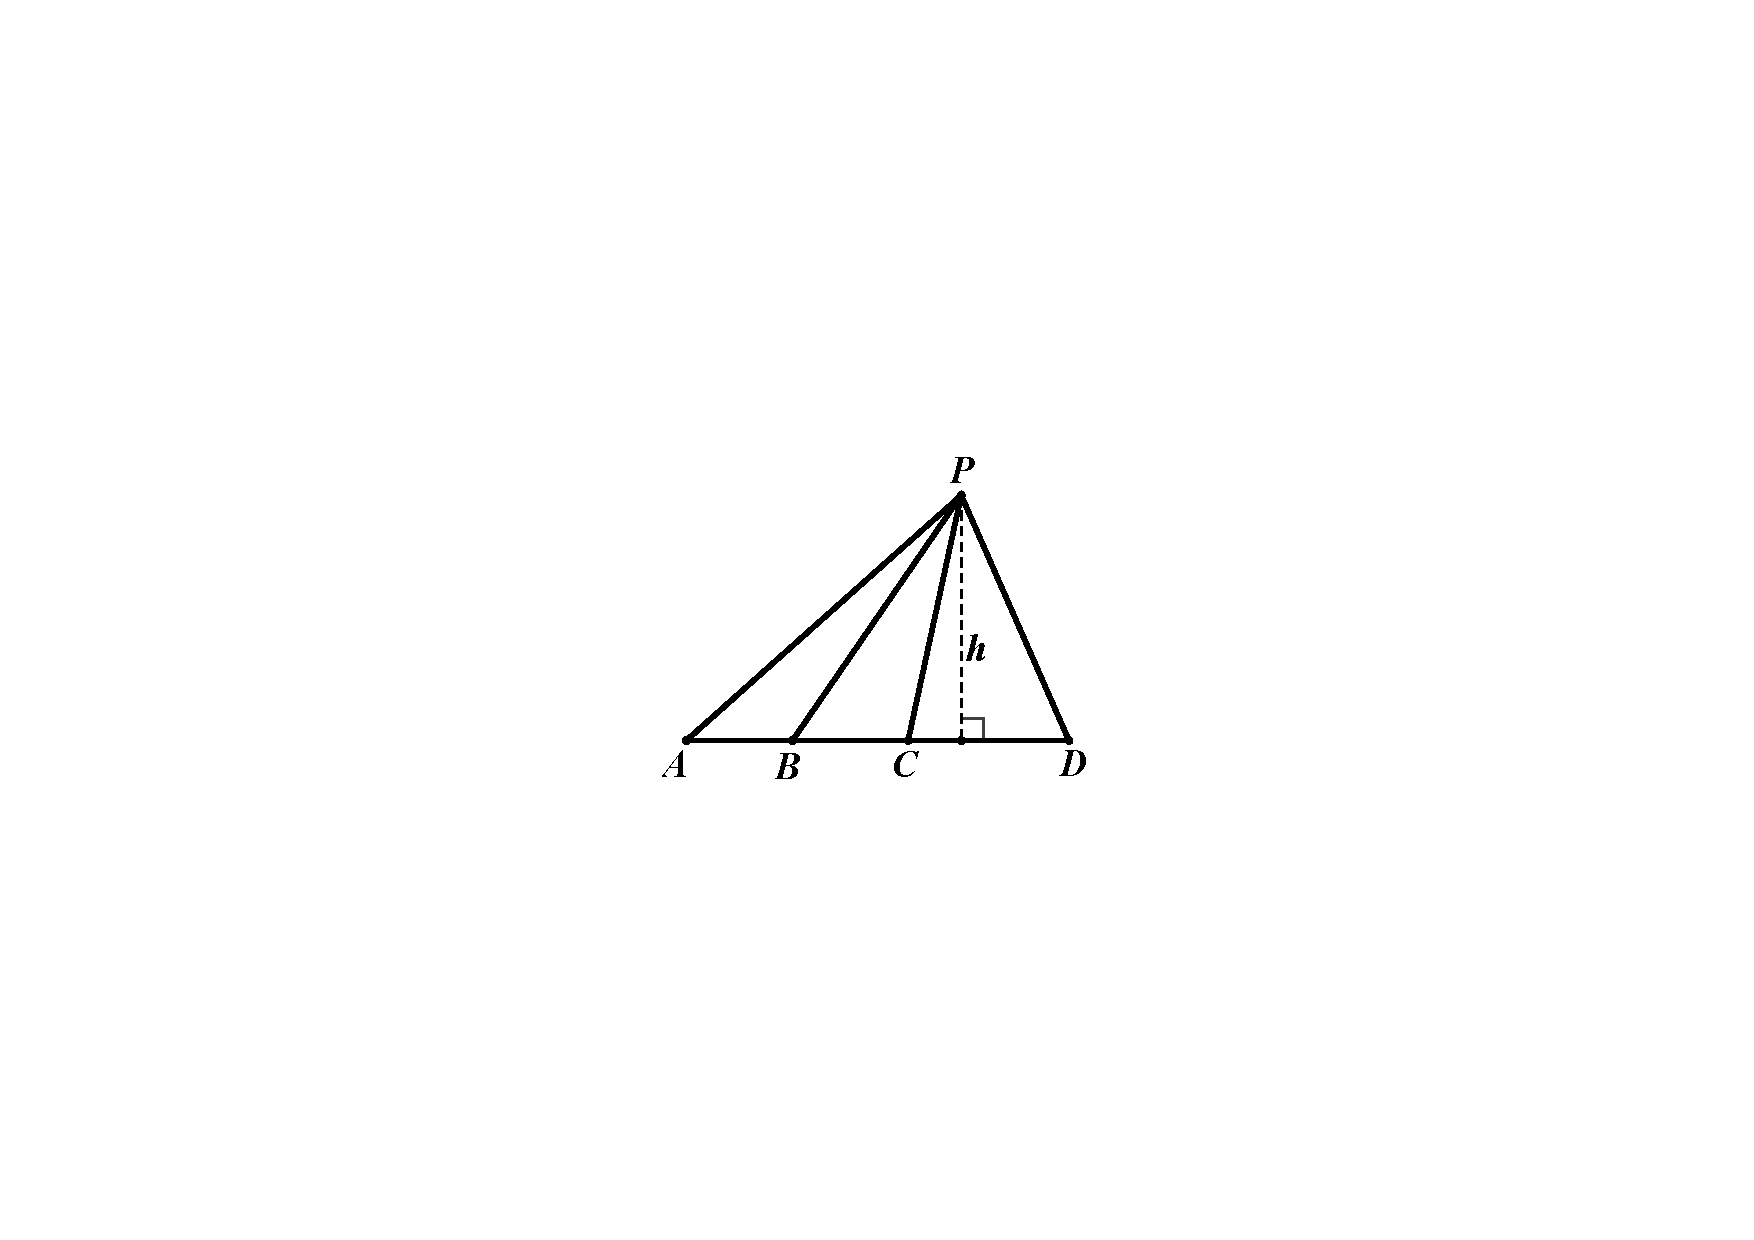
\includegraphics[width=0.3\linewidth]{线段交比等于角度正弦交比}
\end{figure}
\\
\textbf{证}\ 由正弦定理,
\begin{align}
    & \dfrac{|AC|}{\sin\angle APC}=\dfrac{|PA|}{\sin\angle PCA}
    =\dfrac{|PC|}{\sin\angle PAC} \label{线束交比正弦1} \\
    & \dfrac{|BD|}{\sin\angle BPD}=\dfrac{|PB|}{\sin\angle PDB} 
    =\dfrac{|PD|}{\sin\angle PBD} \label{线束交比正弦2}\\
    & \dfrac{|AD|}{\sin\angle APD}=\dfrac{|PD|}{\sin\angle PAC}
    =\dfrac{|PA|}{\sin\angle PDB} \label{线束交比正弦3}\\    
    & \dfrac{|BC|}{\sin\angle BPC}=\dfrac{|PC|}{\sin\angle PBC}
    =\dfrac{|PB|}{\sin\angle PCB} \label{线束交比正弦4}
\end{align}
设$ h $代表$ P $到$ A,B,C,D $所在直线的距离,所以,
\begin{align*}
    \dfrac{\dfrac{|AC|}{\sin\angle APC}\cdot \dfrac{|BD|}{\sin\angle BPD}}
    {\dfrac{|AD|}{\sin\angle APD}\cdot \dfrac{|BC|}{\sin\angle BPC}} &=
    \dfrac{\dfrac{|PA|}{\sin\angle PCA}\cdot \dfrac{|PB|}{\sin\angle PDB}}
    {\dfrac{|PD|}{\sin\angle PAC}\cdot \dfrac{|PC|}{\sin\angle PBC}} \\
    &=\dfrac{|PA|\sin\angle PAC\cdot |PB|\sin\angle PBC}
    {|PD|\sin\angle PDB\cdot |PC|\sin\angle PCA}=\dfrac{h\cdot h}{h\cdot h}=1 
\end{align*}
上面的计算使用了(\ref{线束交比正弦1})$ \sim $(\ref{线束交比正弦4})式的中间一列,
当然也可以使用最右边的列,请读者自行完成。

\item 设圆$ O $是单位圆,$ A,B,C $为圆周上不同的三点,且$ C $点位于劣弧
$ AB $上(弧长小于半圆),$ \vec{OA},\vec{OB} $的夹角为
$ \theta\ (0<\theta<\pi) $,向量$\vec{OC}$与$ \vec{OA},
\vec{OB} $的夹角分别为$ t\theta,(1-t)\theta $,其中$ 0<t<1 $,
设$ \vec{OC}=\lambda\vec{OA}+\mu\vec{OB} $,求$ \lambda,\mu $.
\begin{figure}[h]
    \centering
    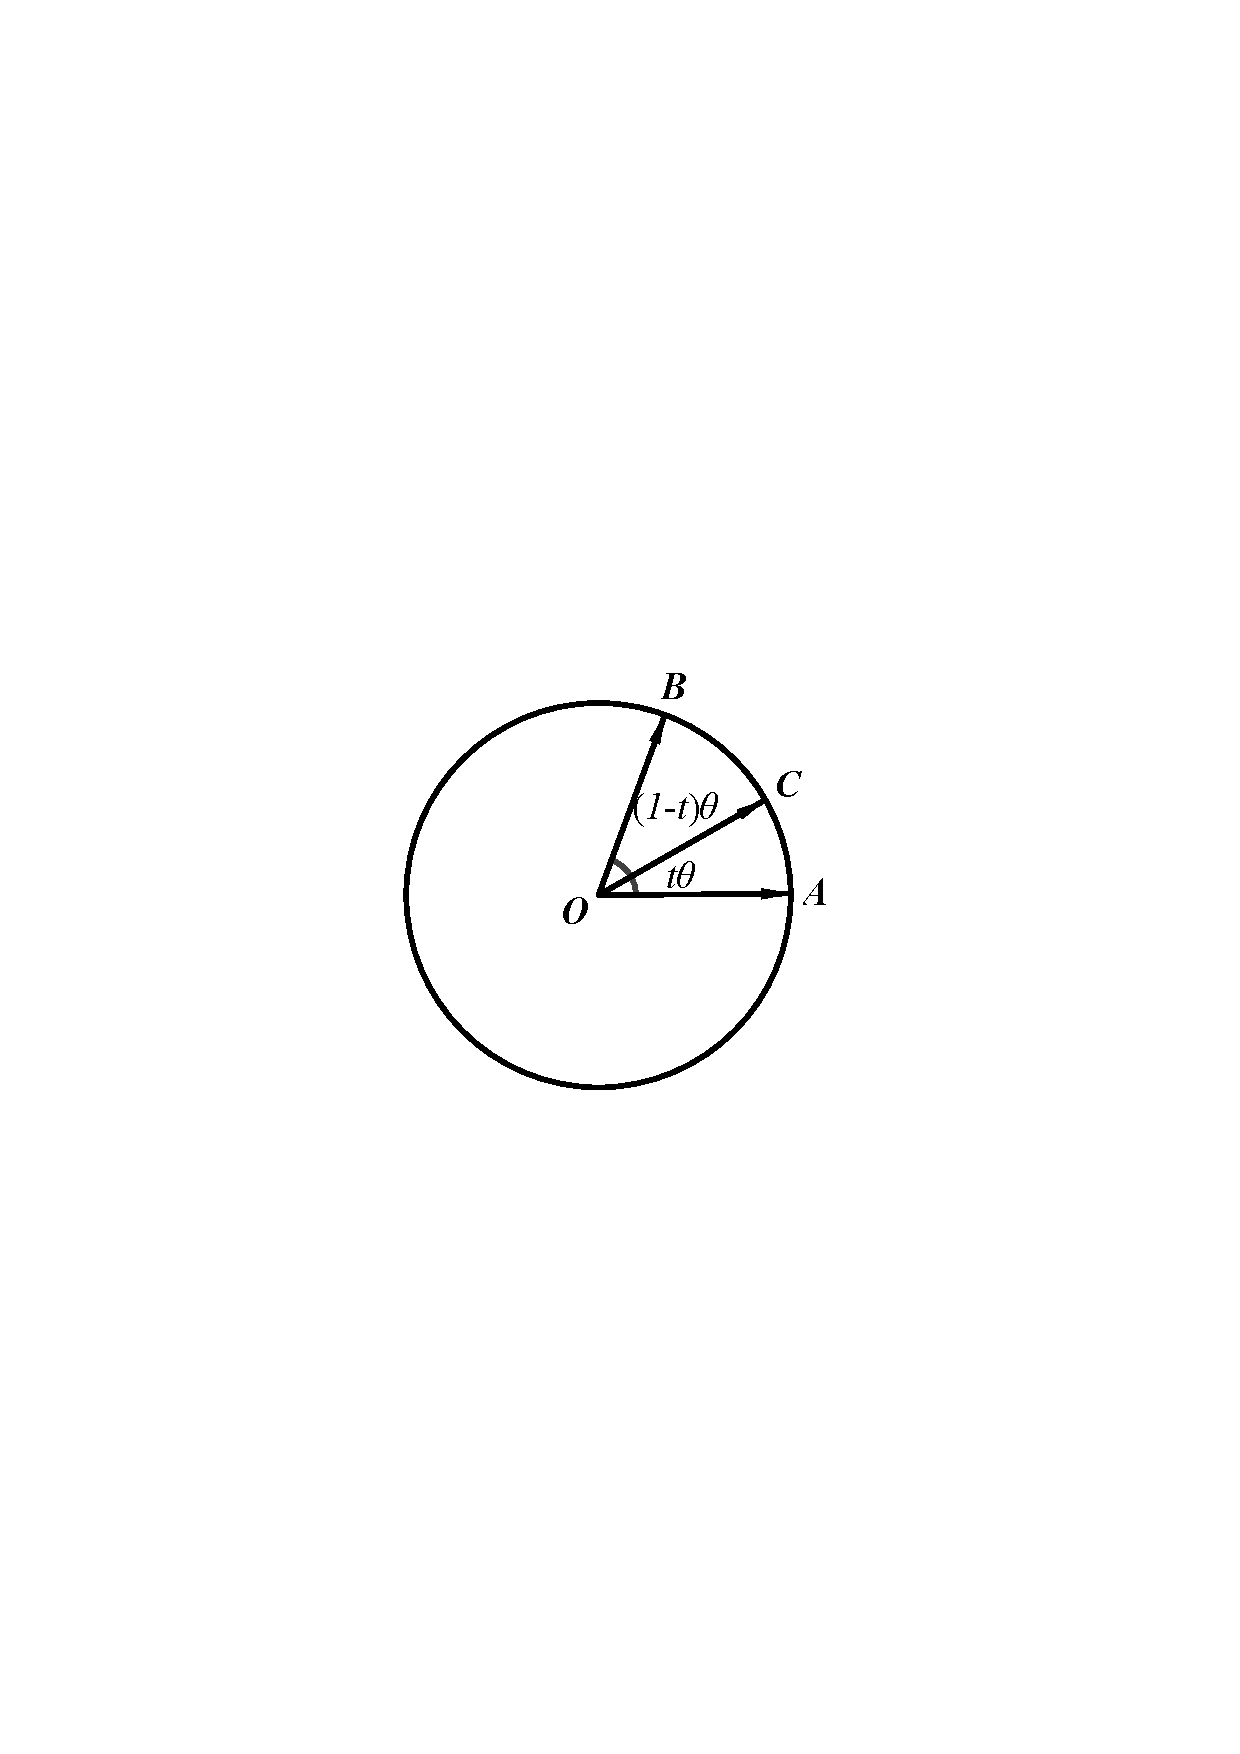
\includegraphics[width=0.3\linewidth]{单位圆上3个向量v1v2合成v四元数背景}
\end{figure} \\
\textbf{解}\ 过$ C $ 点作$ OB $的平行线,与$ OA $交于$ D $点,
则$ \vec{OC}=\vec{OD}+\vec{DC}=\lambda\vec{OA}+\mu\vec{OB} $,
在$ \Delta ODC $中应用正弦定理,
\begin{figure}[h]
    \centering
    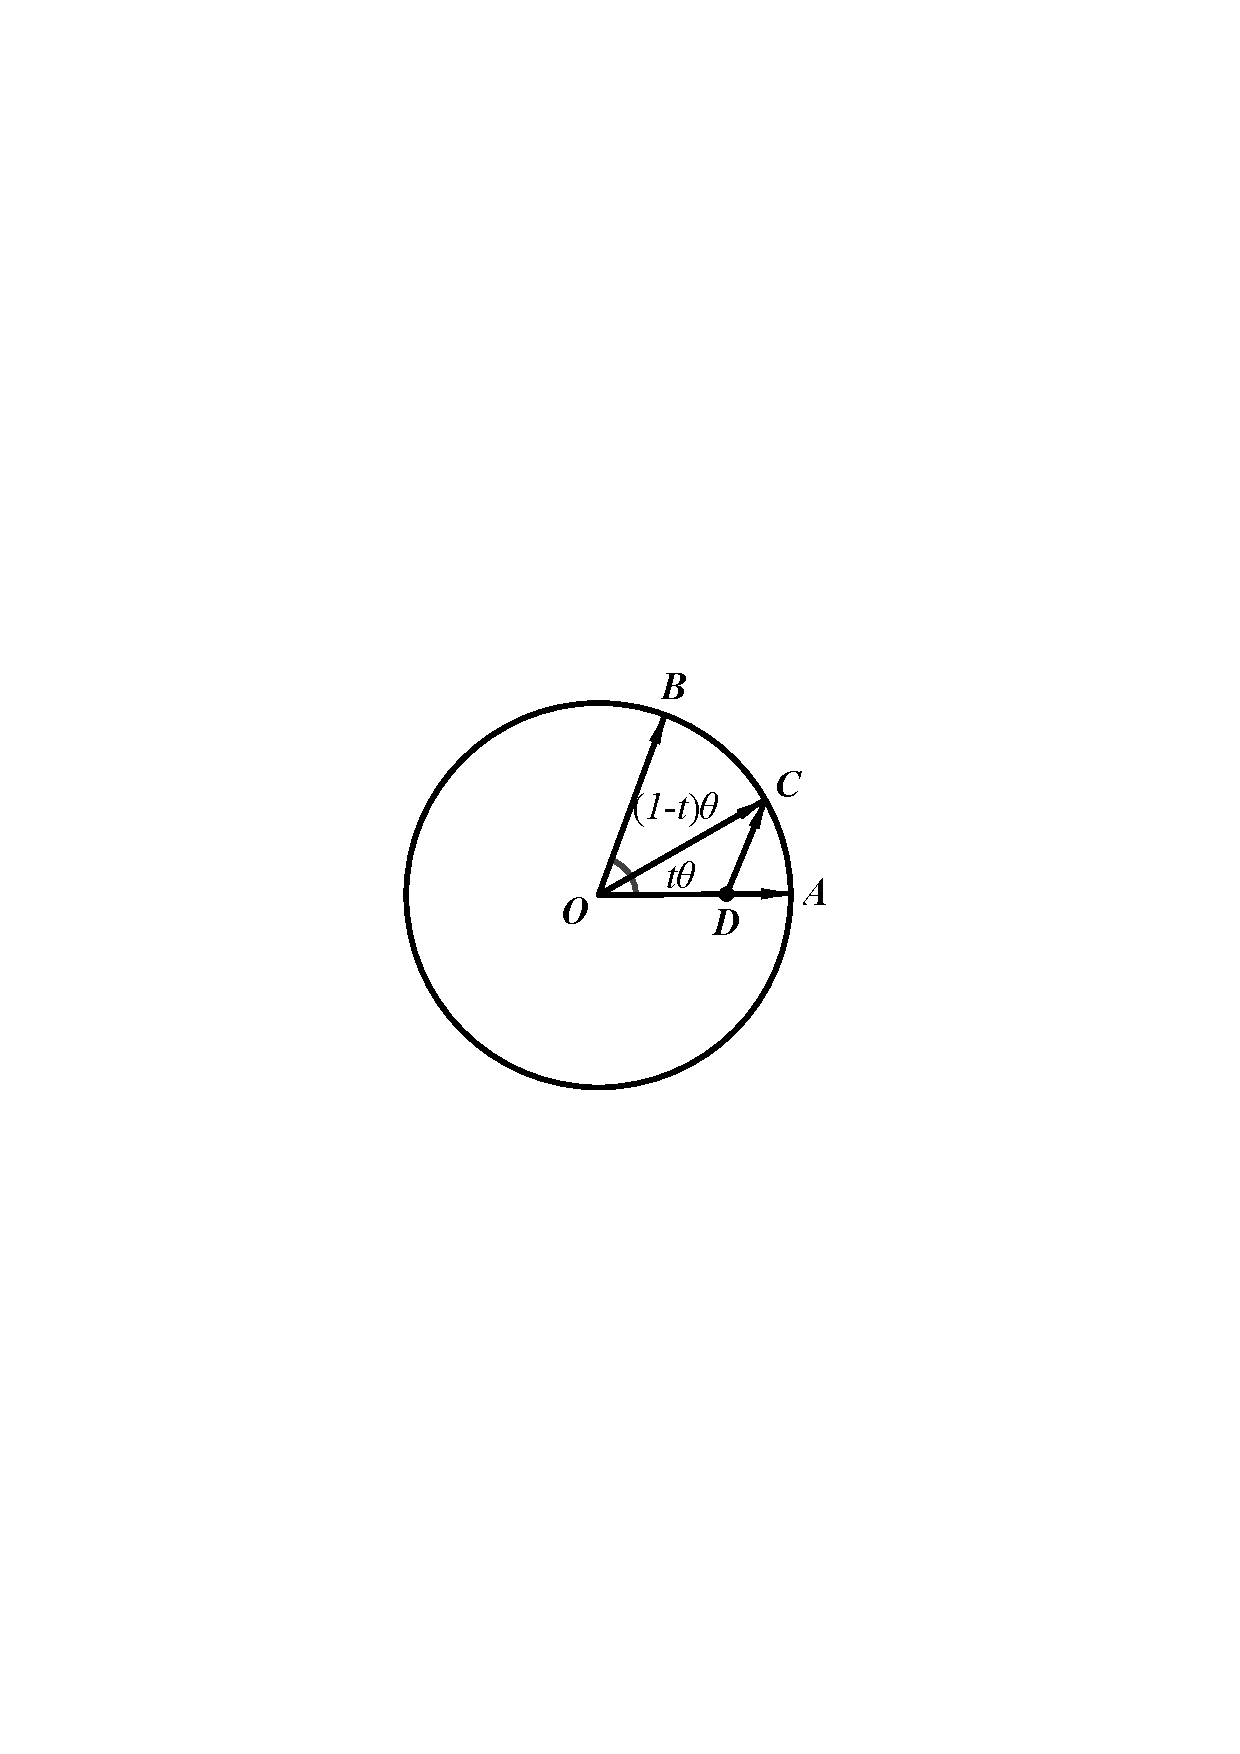
\includegraphics[width=0.3\linewidth]{单位圆上3个向量v1v2合成v四元数背景-含辅助线}
    \label{单位圆上3个向量v1v2合成v}
\end{figure}
\begin{gather*}
    \dfrac{|OC|}{\sin\angle ODC}=\dfrac{|OD|}{\sin\angle OCD}
    =\dfrac{|DC|}{\sin\angle COD} \\
    \dfrac{1}{\sin(\pi-\theta)}=
    \dfrac{\lambda}{\sin((1-t)\theta)}=
    \dfrac{\mu}{\sin(t\theta)}
\end{gather*}
所以,$ \lambda=\dfrac{\sin((1-t)\theta)}{\sin(\theta)},\ 
\mu=\dfrac{\sin(t\theta)}{\sin(\theta)} $. \\
\textbf{注}\ 如果读者以后学习四元数(Quaternion)插值,就会遇到公式
\begin{gather}\label{四元数插值}
    \vec{OC}=\dfrac{\sin((1-t)\theta)}{\sin(\theta)}
    \vec{OA}+\dfrac{\sin(t\theta)}{\sin(\theta)}\vec{OB} 
\end{gather}
如果$ A $、$ C $、$ B $三点共线,那么
\begin{gather}\label{三点共线系数和为1}
    \vec{OC}=(1-\lambda)\vec{OA}+\lambda\vec{OB}
\end{gather}
读者是否注意到了\eqref{三点共线系数和为1}式与
\eqref{四元数插值}式的相似之处?事实上,利用
罗必塔法则\eqref{罗必塔法则}式,
\begin{gather*}
    \lim_{\theta\to 0}\dfrac{\sin((1-t)\theta)}{\sin(\theta)}=
    \lim_{\theta\to 0}\dfrac{(1-t)\cos((1-t)\theta)}{\cos(\theta)}
    =1-t \\
    \lim_{\theta\to 0}\dfrac{\sin(t\theta)}{\sin(\theta)}=
    \lim_{\theta\to 0}\dfrac{t\cos(t\theta)}{\cos(\theta)}
    =t
\end{gather*}
即,\eqref{三点共线系数和为1}式就是\eqref{四元数插值}式在
$ \theta\to 0 $时的极限,当圆弧无限短时,可以认为圆弧就是线段了。

\item $^*$ 设平面$ \alpha $为复平面,$ O $为坐标原点,以$ O $为球心作一个
半径为1的球面。复平面$ \alpha $上有两点$ A,B $,这两点对应的复数
分别为$ z_1,z_2 $. 线段$ ON\perp\alpha $且$ N $点位于球面
($ N $为球的北极点),
$ N,A $所在直线交球面于$ A' $点,$ N,B $所在直线交球面于$ B' $点。
求线段$ |A'B'| $的长度(用含$ z_1,z_2 $的式子表示。) 
\begin{figure}[!ht]
    \centering
    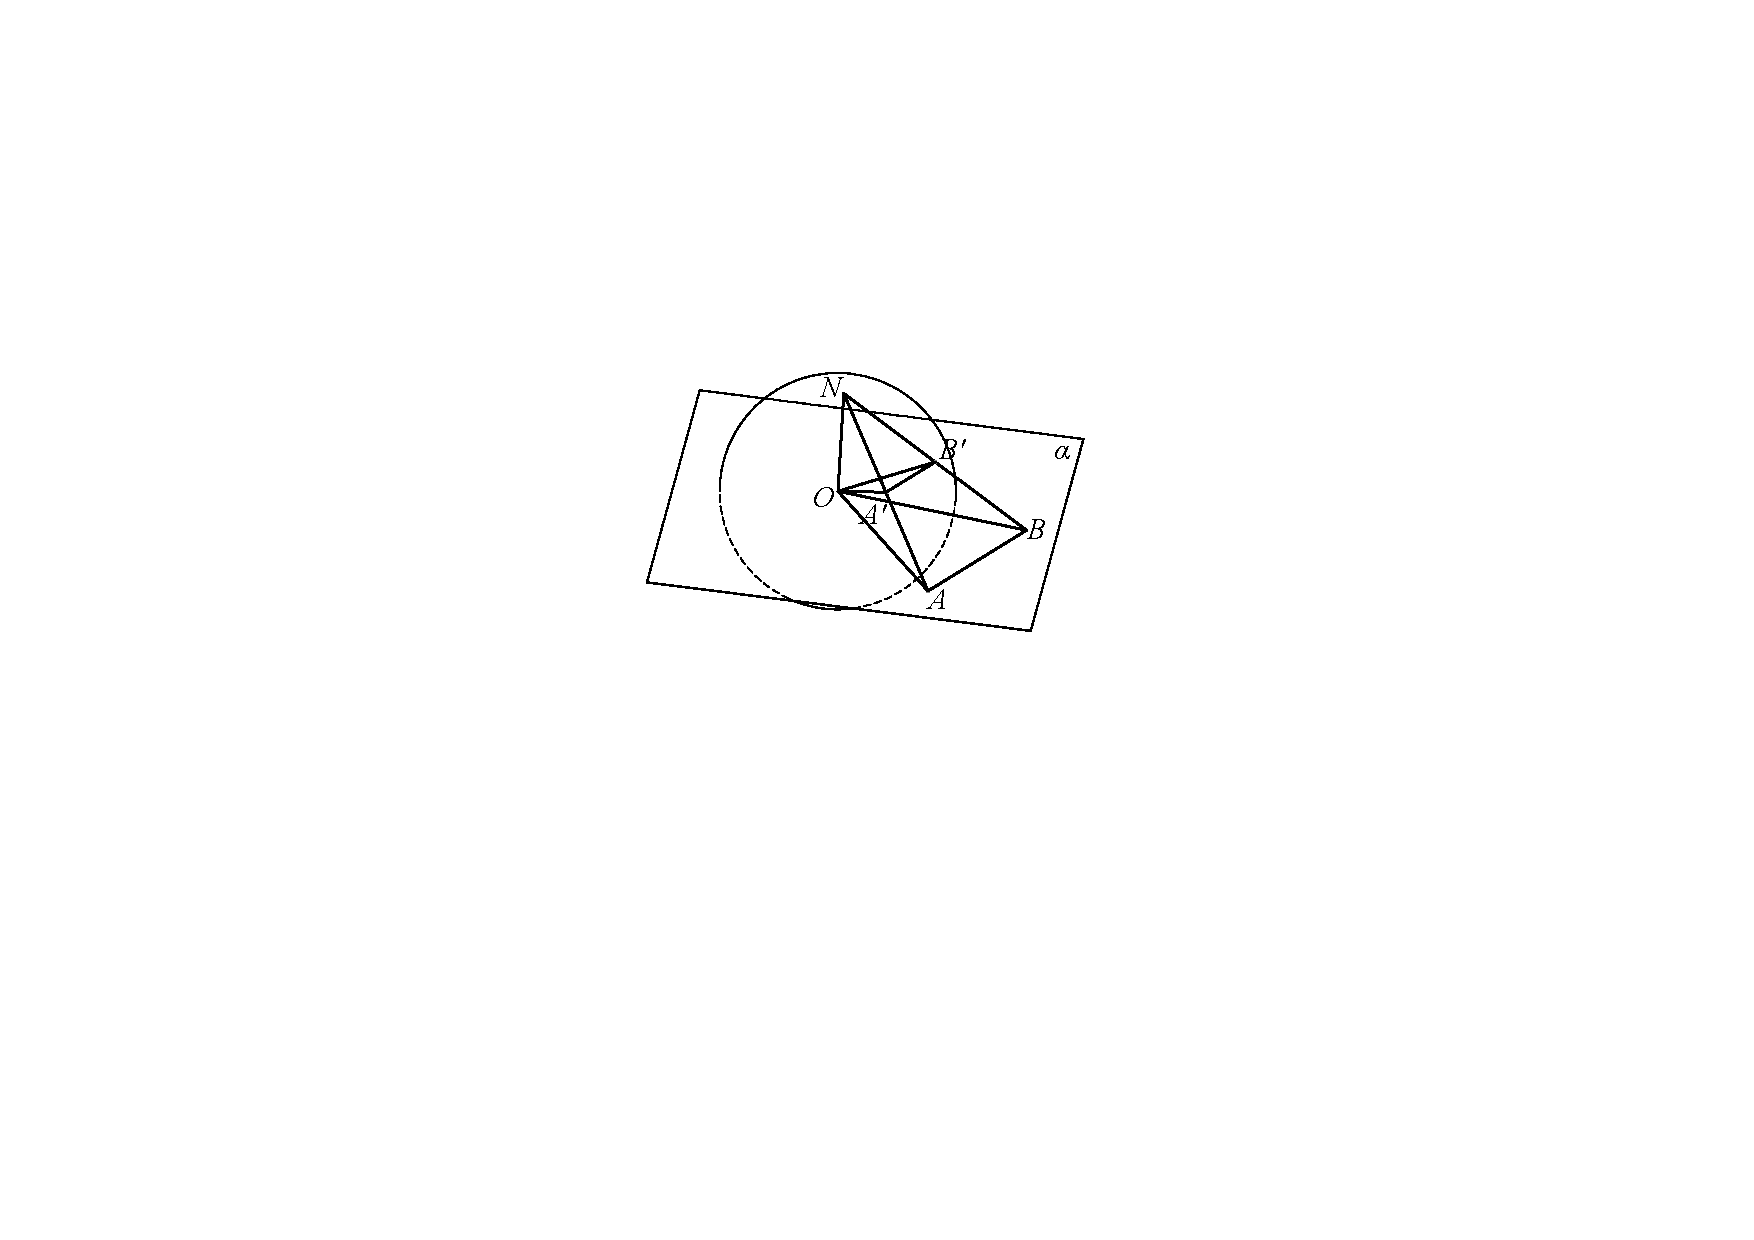
\includegraphics[width=0.5\linewidth]{黎曼球面度量}
\end{figure}
\\
\textbf{解}\ 因为$ |ON|=|OA'|=|OB'|=1 $,所以$ \Delta ONA',
\Delta ONB' $均为等腰三角形,且
\begin{align*}
    |NA'| =2\cos\angle ONA=\dfrac{2}{|NA|},\qquad
    |NB'| =2\cos\angle ONB=\dfrac{2}{|NB|} 
\end{align*}
在$ \Delta NAB $和$ \Delta NA'B' $中使用余弦定理,有
\begin{align*}
    |A'B'|^2 &=|NA'|^2+|NB'|^2-2|NA'|\cdot|NB'|\cos\angle ANB \\
    &=|NA'|^2+|NB'|^2-2|NA'|\cdot|NB'|
    \dfrac{|NA|^2+|NB|^2-|AB|^2}{2|NA|\cdot|NB|} \\
    &=\dfrac{4}{|NA|^2}+\dfrac{4}{|NB|^2}-
    \dfrac{4(|NA|^2+|NB|^2-|AB|^2)}{|NA|^2\cdot|NB|^2} \\
    &=\dfrac{4|AB|^2}{|NA|^2\cdot|NB|^2} 
\end{align*}
所以
\begin{gather*}
    |A'B'|=\dfrac{2|AB|}{|NA|\cdot|NB|}=
    \dfrac{2|z_1-z_2|}{\sqrt{1+|z_1|^2}\sqrt{1+|z_2|^2}}
\end{gather*}
\textbf{注}\ 事实上,
\begin{gather*}
    \dfrac{|NA'|}{|NB'|}=\dfrac{\dfrac{2}{|NA|}}{\dfrac{2}{|NB|}}
    =\dfrac{|NB|}{|NA|}
\end{gather*} 
所以,$ \Delta NB'A' \backsim \Delta NAB $,也可以利用相似三角形求$ |A'B'| $.\\
\textbf{变体}\ 如果不是球心在复平面上,而是球面与复平面相切于原点$ O $,
$ A',B',ON $定义同上,那么$ |A'B'| $表达式会怎样变化?\footnote{
    \q $ |A'B'|=\dfrac{2|AB|}{|NA|\cdot|NB|}=
    \dfrac{2|z_1-z_2|}{\sqrt{4+|z_1|^2}\sqrt{4+|z_2|^2}} $.  } 

\item $ ^* $
在$ \Delta ABC $中,$ D,E,F $分别是$ BC,AC,AB $上的三等分点,
且$ D $靠近$ C $点,$ E $靠近$ A $点,$ F $靠近$ B $点,
求$ \Delta PQR $与$ \Delta ABC $面积的比值。
\begin{figure}[!ht]
    \centering
    \includegraphics[width=0.7\linewidth]{"1_7面积占比 向量题"}
\end{figure}
\\
\textbf{方法一}\ 向量法:\\
\begin{gather*}
    \vec{AP}=\lambda \left(\dfrac{1}{3}\vec{AC} 
    \right) +(1-\lambda)\vec{AB}=k_1\vec{AD}=k_1\left[
    \dfrac{2}{3}\vec{AC}+\dfrac{1}{3}\vec{AB}\right] \\
    \dfrac{\frac{1}{3}\lambda}{1-\lambda}=\dfrac{2}{1},\ 
    \lambda=\dfrac{6}{7},\ k_1=\dfrac{3}{7} \\
    \vec{AR}=\mu \left(\dfrac{2}{3}\vec{AB} \right) +(1-\mu)\vec{AC}=k_2\vec{AD}=k_2\left[ \dfrac{2}{3}\vec{AC}+
    \dfrac{1}{3}\vec{AB} \right] \\
    \dfrac{\frac{2}{3}\mu}{1-\mu}=\dfrac{1}{2},\ 
    \mu=\dfrac{3}{7},\  k_2=\dfrac{6}{7} 
\end{gather*}
所以,$ P $是$ AR $的中点,同理可得,$ Q $是$ BP $的中点,$ R $是$ CQ $的中点,于是
\begin{gather*}
    \dfrac{S_{\Delta PQR}}{S_{\Delta ABC}} =
    \dfrac{S_{\Delta ABD}}{S_{\Delta ABC}}\cdot 
    \dfrac{S_{\Delta PBR}}{S_{\Delta ABD}}\cdot
    \dfrac{S_{\Delta PQR}}{S_{\Delta PBR}}=
    \dfrac{|BD|}{|BC|}\cdot
    \dfrac{|PR|}{|AD|}\cdot \dfrac{|PQ|}{|PB|}=\dfrac{2}{3}\cdot \dfrac{3}{7}\cdot
    \dfrac{1}{2} =\dfrac{1}{7}
\end{gather*}
\\
\textbf{方法二}\ 相似三角形法:过$ D $作$ CF $的平行线交
$ AB $于$ J $点,过$ R,D $作$ BE $的平行线,交$ AC $于$ K,L $两点,
$ \Delta CLD \sim \Delta CEB $,$ \Delta BJD\sim \Delta BFC $,
\begin{gather*}
    |CL|:|LE|=|CD|:|DB|=1:2,\ |EL|=\dfrac{2}{3}|EC|=
    \dfrac{2}{3}\left(\dfrac{2}{3} |AC|\right) =\dfrac{4}{9}|AC|,\\
    |AP|:|PD|=|AE|:|EL|=3:4 \\
    |BJ|:|JF|=|BD|:|DC|=2:1,\ |JF|=\dfrac{1}{3}|BF|=
    \dfrac{1}{3}\left(\dfrac{1}{3}|AB| \right)=\dfrac{1}{9}|AB|, \\
    |AF|:|FJ|=|AR|:|RD|=|AK|:|KL|=6:1  
\end{gather*}
所以,$ |EK|=\dfrac{1}{3}|AC| $,$ K $是$ EC $中点,
$ P $是$ AR $的中点,剩余步骤同方法一。\\
\textbf{注1}\ 如果把三等分点改成$ n $等分点,那么$     \mu=k_1=\dfrac{n}{n^2-n+1},\ \lambda=k_2=\dfrac{n^2-n}{n^2-n+1} $,
\begin{gather*}
    \dfrac{S_{\Delta PQR}}{S_ {\Delta ABC}} =\dfrac{|BD|}{|BC|}\cdot
    \dfrac{|PR|}{|AD|} \cdot \dfrac{|PQ|}{|PB|}=\dfrac{n-1}{n}
    \cdot(k_2-k_1)\cdot\dfrac{k_2-k_1}{k_2}=\dfrac{(n-2)^2}{n^2-n+1}
\end{gather*}
如果$ n=2 $,那么$ S_{\Delta PQR} =0 $,这正是三条中线交于一点的表现。\\
\textbf{注2}\ 更一般地,若$ \dfrac{|AF|}{|FB|}=\lambda_1,\ 
\dfrac{|BD|}{|DC|}=\lambda_2,\ \dfrac{|CE|}{|EA|}=\lambda_3 $,那么
\begin{align*}
    \dfrac{S_{\Delta PQR}}{S_ {\Delta ABC}} =\dfrac{(\lambda_1\lambda_2
        \lambda_3-1)^2}{(1+\lambda_1+\lambda_1\lambda_2)
        (1+\lambda_2+\lambda_2\lambda_3)(1+\lambda_3+\lambda_3\lambda_1)}
\end{align*}

\item 已知$ \vec{a}=(x,t),\ \vec{b}=(t,y) $,
若$ x,y $是常数,且$ \vec{a},\vec{b} $的夹角为$ \theta $,
求$ t $. \\
\textbf{方法一}\ 设向量$ \vec{a},\vec{b} $所在的直线倾斜角
分别为$ \theta_1,\theta_2 $,由正切差角公式:
\begin{gather*}
    \pm\tan\theta=\tan(\theta_1-\theta_2)=\dfrac{\tan\theta_1-\tan\theta_2}
    {1+\tan\theta_1	\tan\theta_2}=\dfrac{\dfrac{t}{x}-\dfrac{y}{t}}{1+
        \dfrac{t}{x}\cdot\dfrac{y}{t}}=\dfrac{t^2-xy}{xt+yt} 
\end{gather*}
\begin{gather}\label{正切化成的二次方程}
    t^2\pm(\tan\theta)(x+y)t-xy=0
\end{gather}
直接解方程,就能得到$ t $. 
现在让我们站在命题人的角度来看方程(\ref{正切化成的二次方程}),我们希望解出的$ t $
是有理数(不含有根式),最好还是整数,以减小计算量。为满足这个要求,该如何选定$ x,y $呢?
让我们从韦达定理的角度考虑。\\
\ding{192} 方程(\ref{正切化成的二次方程})的两根为$ x,-y $,那么
\begin{gather}\label{考虑有理数-情形1}
    x-y=\pm(\tan\theta)(x+y)
\end{gather}
只要让$ \tan\theta $是有理数,那么当$ x $是有理数时,$ y $也必然是有理数。\\
\ding{193} 方程(\ref{正切化成的二次方程})的两根为$ 1,-xy $,那么
\begin{gather}\label{考虑有理数-情形2}
    1-xy=\pm(\tan\theta)(x+y)
\end{gather}
只要让$ \tan\theta $是有理数,那么当$ x $是有理数时,$ y $也必然是有理数。\\
\ding{194} 方程(\ref{正切化成的二次方程})的两根为$ \sqrt{x},-\sqrt{x}y $,那么
\begin{gather}\label{考虑有理数-情形3}
    \sqrt{x}(1-y)=\pm(\tan\theta)(x+y) 
\end{gather}
只要让$ \tan\theta $是有理数,那么当$ \sqrt{x} $是有理数时,$ y $也必然是有理数。\\
\\
\textbf{方法二}\ $ \cos\theta=\dfrac{tx+ty}{\sqrt{x^2+t^2}\sqrt{y^2+t^2}} $,整理得:
\begin{align}\label{余弦化成t2二次方程}
    t^4+\left[x^2+y^2-\dfrac{1}{\cos^2\theta}(x+y)^2\right]t^2+x^2y^2=0
\end{align}
这是关于$ t^2 $的二次方程。\\
\ding{192} 方程(\ref{余弦化成t2二次方程})的两根为$ x^2,y^2 $,那么
\begin{gather*}
    x^2+y^2=\dfrac{1}{\cos^2\theta}(x+y)^2-(x^2+y^2) \\
    2(x^2+y^2)-(x+y)^2=\dfrac{1}{\cos^2\theta}(x+y)^2 -(x+y)^2 \\
    (x-y)^2=(\tan\theta)^2(x+y)^2
\end{gather*}
这与(\ref{考虑有理数-情形1})式等价。\\
\ding{193} 方程(\ref{余弦化成t2二次方程})的两根为$ 1,x^2y^2 $,那么
\begin{gather*}
    1+x^2y^2=\dfrac{1}{\cos^2\theta}(x+y)^2-(x^2+y^2) \\
    1+x^2y^2-2xy=\dfrac{1}{\cos^2\theta}(x+y)^2-(x^2+y^2+2xy) \\
    (1-xy)^2=(\tan\theta)^2 (x+y)^2 
\end{gather*}
这与(\ref{考虑有理数-情形2})式等价。\\
\ding{194} 方程(\ref{余弦化成t2二次方程})的两根为$ x,xy^2 $,那么
\begin{gather*}
    x+xy^2=\dfrac{1}{\cos^2\theta}(x+y)^2-(x^2+y^2) \\
    x+xy^2-2xy=\dfrac{1}{\cos^2\theta}(x+y)^2-(x^2+y^2+2xy) 
\end{gather*}
\begin{gather}\label{考虑有理数-情形3已平方}
    x(1-y)^2=(\tan\theta)^2(x+y)^2
\end{gather}
这与(\ref{考虑有理数-情形3})式等价。列举一些整数解的情形:$ \tan\theta=3 $,
(\ref{考虑有理数-情形3已平方})式有$ (1,-2),(4,-14) $等整数解;
$ \tan\theta=4 $,(\ref{考虑有理数-情形3已平方})式有$ (4,-9),(9,-39) $等整数解;
$ \tan\theta=5 $,(\ref{考虑有理数-情形3已平方})式有
$ (9,-24),(16,-84) $等整数解。

% FermatPoint_9_16_25_StudyAgain.m
% 
\item \label{三元二次非线性方程组-费马点}正实数$ x,y,z $满足
$ \begin{cases}
    x^2+xy+y^2=9  &\mycircled{1} \\
    y^2+yz+z^2=6  &\mycircled{2} \\
    z^2+zx+x^2=25 &\mycircled{3}
\end{cases} $,求$ xy+yz+zx $的值。\\
\textbf{解}\ $ x,y,z $可看成边长为$ 3,4,5 $的直角三角形的费马点与三个顶点连线的长度,
直角三角形的面积等于三个小三角形面积之和:$ \dfrac{1}{2}\cdot 3\cdot 4= \dfrac{1}{2}\cdot(xy+yz+zx)\sin 120^{\circ} $,于是
$ xy+yz+zx=8\sqrt{3} $. 如果读者第一次遇到此类较难的题目而无从下手,但题目恰好以选择题形式出现,
那么至少可利用基本不等式排除明显错误的答案,因为$ x,y,z $任意两个都不相等
(令其中两个相等,会得到相互矛盾的两个方程),
所以,$ 2xy+xy < x^2+y^2+xy =9,\ xy <3$,同理可得,$ yz<\dfrac{16}{3},zx<\dfrac{25}{3} $,
于是$ xy+yz+zx < \dfrac{50}{3} $,所有大于等于$ \dfrac{50}{3}=16.66\cdots $
的选项均可排除。$ (8\sqrt{3}\approx 13.8564 ) $. \\
如果将\mycircled{1},\mycircled{2},\mycircled{3}
式等号右侧的常数分别换成$ a^2,b^2,c^2\ 
(a+b>c>0,b+c>a>0,c+a>b>0) $,
那么利用海伦公式可得
\begin{gather*}
    xy+yz+zx=
    \dfrac{4}{\sqrt{3}}S_{\Delta ABC}=
    \dfrac{4}{\sqrt{3}}\sqrt{p(p-a)(p-b)(p-c)}, \q 
    \left(p=\dfrac{a+b+c}{2} \right)
\end{gather*}
又有
\begin{gather*}
    xy+yz+zx\leq \dfrac{1}{3}(a^2+b^2+c^2)
\end{gather*}
等号在$ a=b=c $时成立。以上不等式还可以从另一个角度理解,
结合$ xy+yz+zx=\dfrac{4}{\sqrt{3}}S_{\Delta ABC} $与外森比克不等式
(\ref{外森比克不等式}),
\begin{gather*}
    S_{\Delta ABC}\leq \dfrac{1}{4\sqrt{3}}(a^2+b^2+c^2) \\
    xy+yz+zx=\dfrac{4}{\sqrt{3}}S_{\Delta ABC}\leq 
    \dfrac{4}{\sqrt{3}}\cdot \dfrac{1}{4\sqrt{3}}(a^2+b^2+c^2)=
    \dfrac{1}{3}(a^2+b^2+c^2)
\end{gather*}

如果想在只有计算器的情况下求这个方程组的近似解,
可用消元法转化为关于一个变量的方程,然后用二分法求解。
例如,由\mycircled{1}可得$ x=\dfrac{1}{2}(-y\pm\sqrt{36-3y^2}) $,由\mycircled{2}可得
$ z=\dfrac{1}{2}(-y\pm\sqrt{64-3y^2}) $,将$ x,z $的表达式(只考虑取正根的情况)带入\mycircled{3},整理后可得:
\begin{align}\label{费马点例题f(y)=3y2+3y}
    f(y)=3y^2+3y\left(\sqrt{36-3y^2}+\sqrt{64-3y^2}\right)
    -\sqrt{36-3y^2} \sqrt{64-3y^2}=0
\end{align}
此方程已经可以通过二分法求解(也可用GeoGebra求零点)。当然,还可以多次进行平方与移项操作,
消去所有的根号,得到一个关于$ y $的高次方程。解出$ y $以后就立刻能得到$ x,z $. 
但如果只是要得到$ xy+yz+zx $的近似值,是可以不直接使用$ x,z $的值的,这是因为
\begin{align*}
    &\ xy+yz+zx=(x+z)y+zx\\ =&\ \dfrac{1}{4}
    \left[-3y^2+y\left(\sqrt{36-3y^2}+\sqrt{64-3y^2}\right)  
    +\sqrt{36-3y^2}\cdot \sqrt{64-3y^2}\right]\ 
    (\text{利用}(\ref{费马点例题f(y)=3y2+3y})\text{化简})\\ 
    =&\ y\left(\sqrt{36-3y^2}+\sqrt{64-3y^2}\right)
\end{align*}

通过求导,可算出 $ f(y) $的极小值点为
$ \left( -\dfrac{12}{\sqrt{37}},-96\right) $,极大值点为
$ \left(\dfrac{12}{\sqrt{13}},96\right) $,$ f(y) $的图像如下,形状像一把勺子,
并不具有任何对称性,但极大值和极小值的绝对值相同,还是令人有些诧异。
感兴趣的读者还可尝试利用初等方法(不借助导数)寻找$ f(y) $的极值。 
\begin{figure}[h] % xy_yz_zxFermat.m
    \centering
    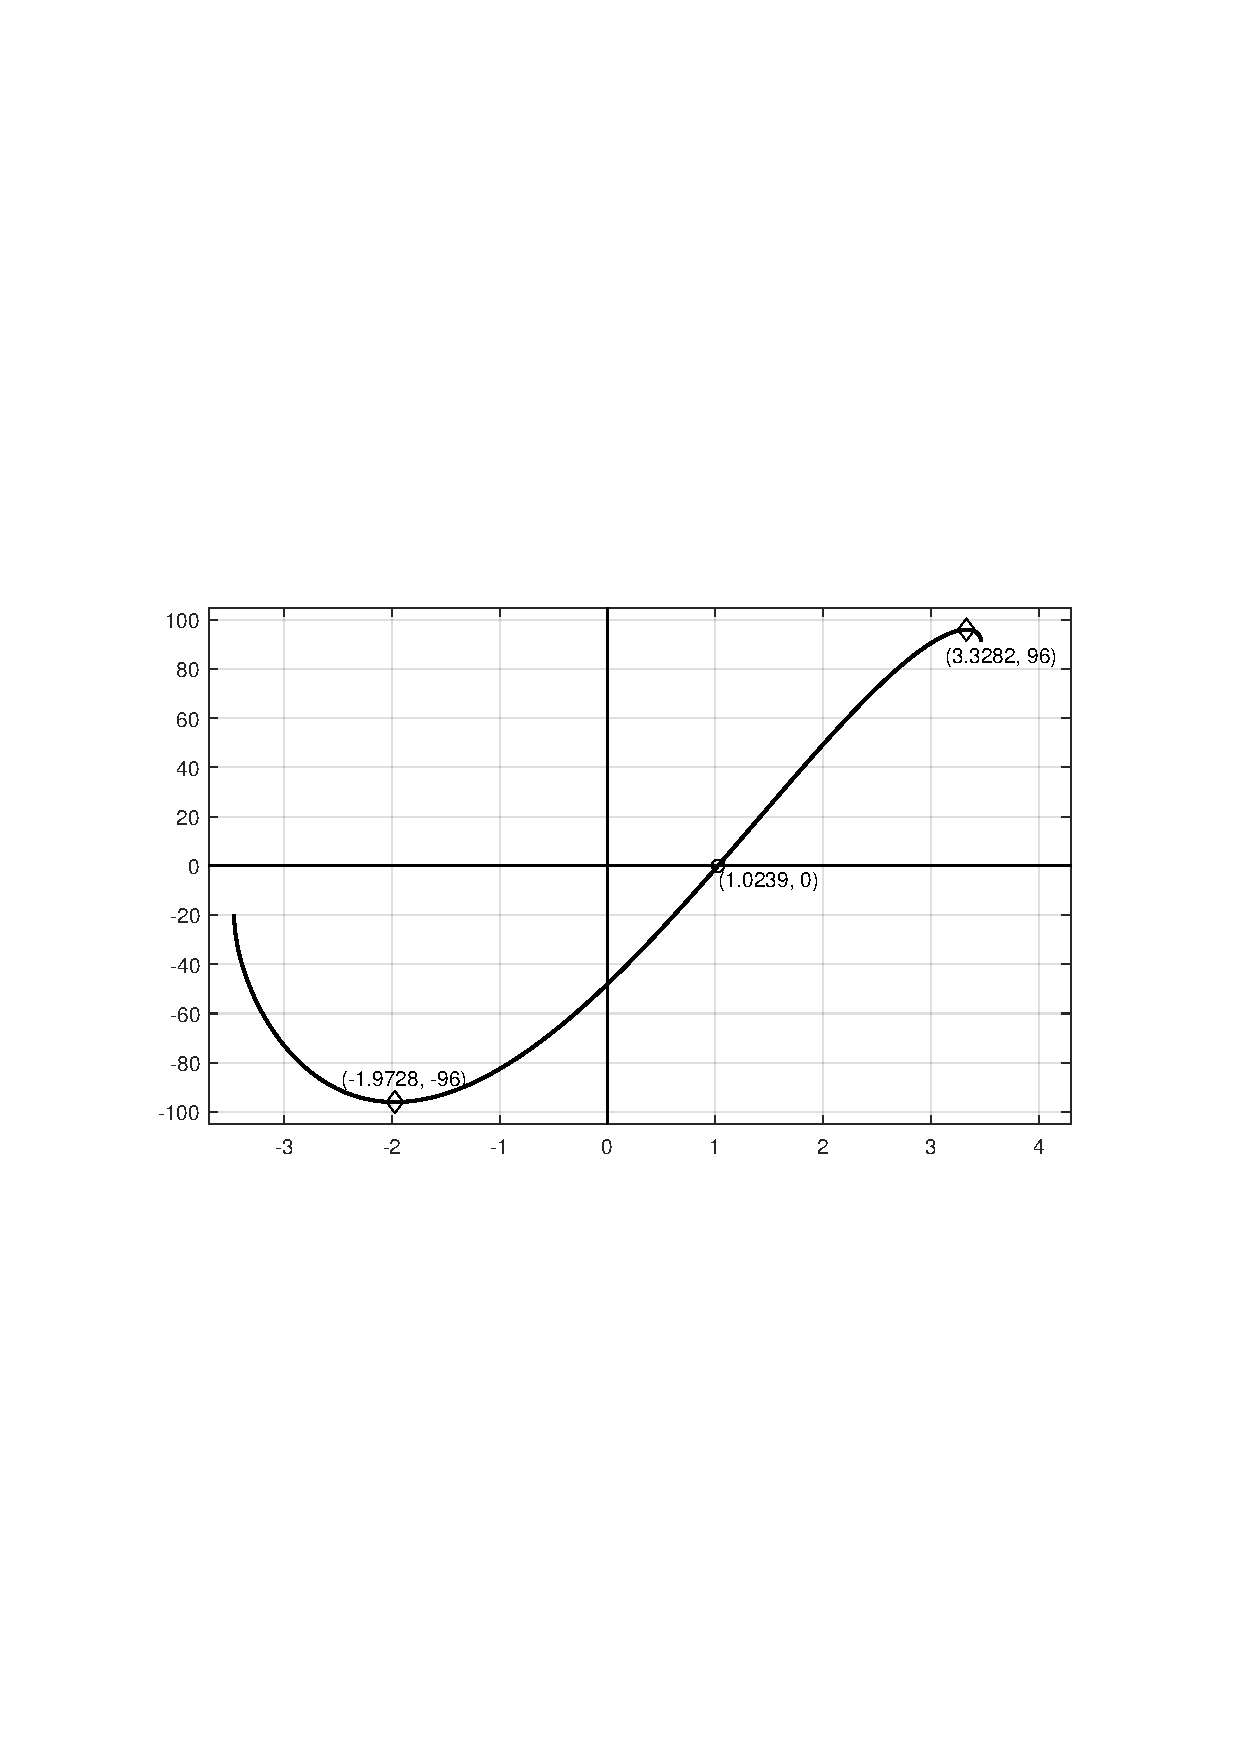
\includegraphics[width=0.6\linewidth]{xy+yz+zx题目}
\end{figure}

下面介绍由\mycircled{1}、\mycircled{2}、\mycircled{3}
组成的方程组的直接求解方法,
将$ 9,16,25 $换成一般性的常数$ a^2,b^2,c^2 $,(不要求$ a^2+b^2=c^2 $,
只要求以$ |a|,|b|,|c| $为边长能构成三角形。)
分别用$ \mycircled{1}-\mycircled{2},
\mycircled{1}-\mycircled{3},\mycircled{2}-\mycircled{3} $,
(这一方法已经在第\pageref{复数多元二次方程求解演示} 
页的\ref{复数多元二次方程求解演示}的方法三中演示过了,
形式一致的式子相减,往往可以因式分解),可得:
\begin{align*}
    \begin{cases}
        (x+y+z)(x-z)= a^2-b^2 \q \mycircled{4}  \\
        (x+y+z)(y-z)= a^2-c^2 \q \mycircled{5}  \\
        (x+y+z)(y-x)= b^2-c^2 \q \mycircled{6} 
    \end{cases}
\end{align*}
以上三式左右同时平方后相加,可得:
\begin{gather*}
    \left[ x^2+y^2+z^2+2(xy+yz+zx) \right] \left[ 2(x^2+y^2+z^2)-2(xy+yz+zx) \right] \\
    =2(a^4+b^4+c^4)-2(a^2b^2+b^2c^2+c^2a^2) \hspace{1cm} \mycircled{7}
\end{gather*}
由 \mycircled{1}+\mycircled{2}+\mycircled{3} 可得
\begin{align*}
    2(x^2+y^2+z^2)+(xy+yz+zx)=a^2+b^2+c^2  \hspace{1cm} \mycircled{8}
\end{align*}
记
\begin{align*}
    & s_1=x+y+z \\
    & s_2=x^2+y^2+z^2 \\
    & \sigma_2=xy+yz+zx  \\
    & u=a^4+b^4+c^4 \\
    & v=a^2b^2+b^2c^2+c^2a^2 \\
    & w=a^2+b^2+c^2
\end{align*}
那么$ w^2=u+2v $,\mycircled{7}、\mycircled{8}两式成为
\begin{align*}
    \begin{cases}
        (s_2+2\sigma_2)(2s_2-2\sigma_2)= 2u-2v \\
        2s_2+\sigma_2 = w
    \end{cases}
\end{align*}
解得:
\begin{align*}
    \begin{cases}
        s_2 = \dfrac{1}{2}\left[w \mp \sqrt{\dfrac{-u+2v}{3}}\right] \\
        \sigma_2= \pm \sqrt{\dfrac{-u+2v}{3}}=
        \pm \dfrac{4}{\sqrt{3}}\sqrt{\dfrac{-u+2v}{16}}=
        \pm\dfrac{4}{\sqrt{3}}S_{\Delta ABC} 
        %    =\pm \dfrac{4}{\sqrt{3}}\sqrt{p(p-a)(p-b)(p-c)}
    \end{cases}
\end{align*}
所以,
\begin{gather*}
    s_1=x+y+z=\pm\sqrt{s_2+2\sigma_2 }=
    \pm \sqrt{\dfrac{1}{2}[w\pm\sqrt{3(-u+2v)}]}
\end{gather*}
根据\mycircled{4}式,$ s_1(x-z)=a^2-b^2 $,
有$ z=x+\dfrac{b^2-a^2}{s_1} $;\\
同理,根据\mycircled{6}式,有$ y=x+\dfrac{b^2-c^2}{s_1} $,于是
\begin{gather*}
    x+y+z=3x+\dfrac{2b^2-a^2-c^2}{s_1}=s_1 \\
    \begin{cases}
        x=\dfrac{1}{3}\left(s_1+\dfrac{a^2+c^2-2b^2}{s_1}\right)\\[3mm]
        y=\dfrac{1}{3}\left(s_1+\dfrac{a^2+b^2-2c^2}{s_1}\right)\\[3mm]
        z=\dfrac{1}{3}\left(s_1+\dfrac{b^2+c^2-2a^2}{s_1}\right)
    \end{cases}
\end{gather*}
当$ a,b,c $分别为$ 3,\ 4,\ 5 $时,若限制$ x,y,z $均为正数,则
\begin{gather*}
\begin{cases}
    \sigma_2 =8\sqrt{3} \\        
    s_2 =25- 4\sqrt{3} \\
    s_1=\sqrt{25 + 12\sqrt{3}}
\end{cases}
\Rightarrow 
\begin{cases}
    x =\dfrac{1}{3}\left(\sqrt{25 + 12\sqrt{3}}+
    \dfrac{2}{\sqrt{25 + 12\sqrt{3}}}\right)=2.35400309 \cdots\\
    y =\dfrac{1}{3}\left(\sqrt{25 + 12\sqrt{3}}-
    \dfrac{25}{\sqrt{25 + 12\sqrt{3}}}\right)= 1.02390782 \cdots\\
    z =\dfrac{1}{3}\left(\sqrt{25 + 12\sqrt{3}}+
    \dfrac{23}{\sqrt{25 + 12\sqrt{3}}}\right)= 3.38852164 \cdots 
\end{cases}
\end{gather*}
若允许$ x,y,z $出现负数,则还有如下一组解:
\begin{align*}
    \begin{cases}
        \sigma_2 = -8\sqrt{3} \\        
        s_2 = 25+ 4\sqrt{3} \\
        s_1=\sqrt{25 - 12\sqrt{3}}
    \end{cases}
    \Rightarrow 
    \begin{cases}
        x =\dfrac{1}{3}\left(\sqrt{25 - 12\sqrt{3}}+
        \dfrac{2}{\sqrt{25 - 12\sqrt{3}}}\right)=1.00908617 \cdots \\
        y =\dfrac{1}{3}\left(\sqrt{25 - 12\sqrt{3}}-
        \dfrac{25}{\sqrt{25 - 12\sqrt{3}}}\right)=-3.37444009 \cdots \\
        z =\dfrac{1}{3}\left(\sqrt{25 - 12\sqrt{3}}+
        \dfrac{23}{\sqrt{25 - 12\sqrt{3}}}\right)= 4.41849548 \cdots 
    \end{cases}
\end{align*}
当然,如果把$ x,y,z $全部变成相反数,也是原方程组的解。
\footnote{注:$ \sqrt{25\pm 12\sqrt{3}} =\dfrac{1}{2}\left(\sqrt{50+2\sqrt{193}}
    \pm \sqrt{50-2\sqrt{193}}\right) $,无法去掉外层根号。}

\begin{figure}[H]
    \centering
    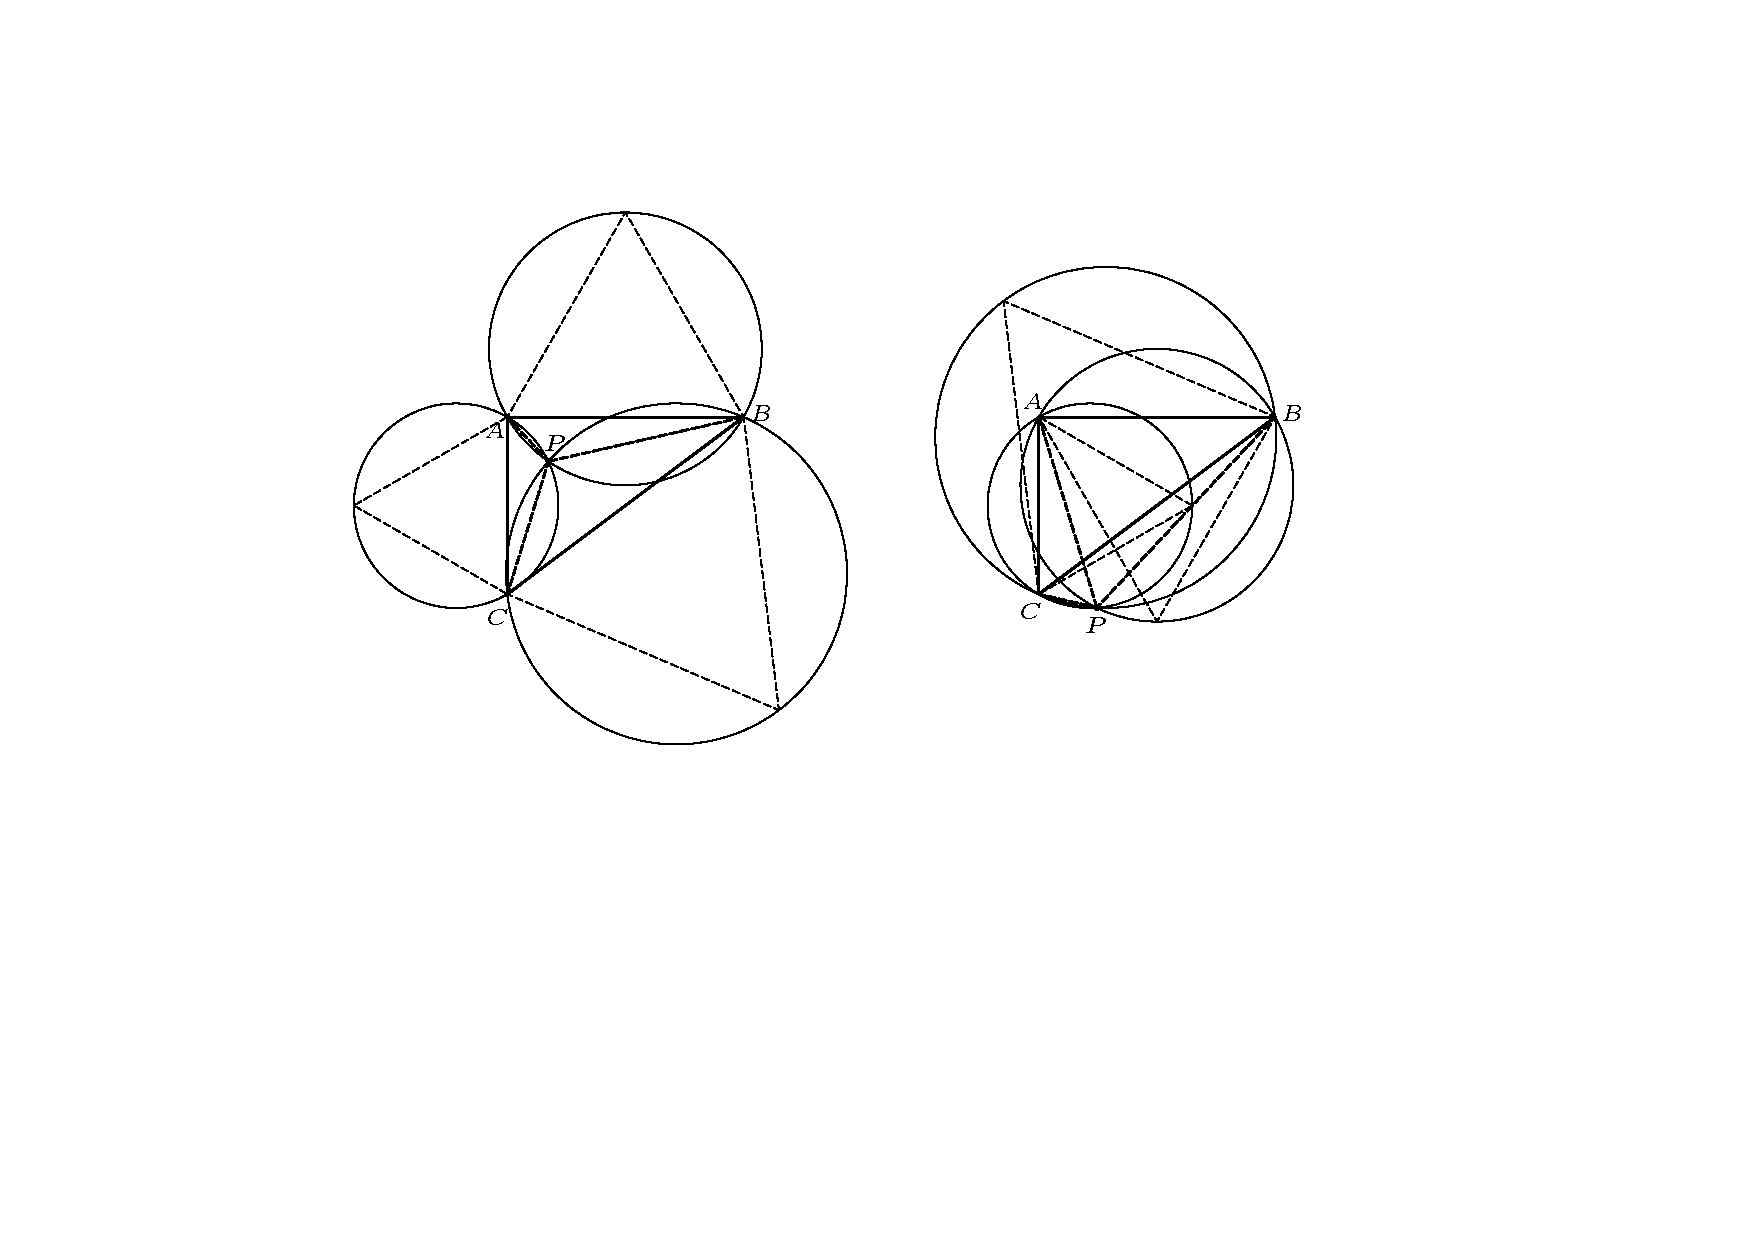
\includegraphics[width=0.75\linewidth]{费马点3-4-5}
\end{figure} 
第一组解对应上面左图的情形:向$ \Delta ABC $外部作等边三角形,三个外接圆交点
$ P $在$ \Delta ABC $内部,$ \angle APB=\angle BPC =\angle CPA
=120^{\circ} ,S_{\Delta ABC}=S_{\Delta APB}+S_{\Delta BPC}+S_{\Delta CPA}$.
第二组解对应上面右图的情形:向$ \Delta ABC $内部作等边三角形,
三个外接圆交点$ P $在$ \Delta ABC $外部,$ \angle APB=\angle APC
=60^{\circ},\angle BPC=120^{\circ},S_{\Delta ABC}=S_{\Delta APB}+
S_{\Delta APC}-S_{\Delta BPC} $. 在两张图中都有:
$ |AC|=3,|AB|=4,|BC|=5, |PC|=|x|,|PA|=|y|,|PB|=|z| $. 


方程\mycircled{1}、\mycircled{2}、\mycircled{3}还可以看成三维空间中
三个两两相互垂直的椭圆柱面,感兴趣的可以用GeoGebra画图看看。
关于$ x+y+z $还有如下不等式\footnote{证明过程可查阅:张善立.
    有关费尔马点的一个不等式的加强[J]. 中等数学, 1997(04):22-22.}:
\begin{gather*}
    x+y+z\leq \sqrt{ab+bc+ca}
\end{gather*} 

\item $ ^* $ \label{2010江西高考}
(2010,江西高考)证明以下命题:\\
(I)对任意正整数$ a $ ,都存在正整数$ b,c\ (b<c) $,使得$ a^2,b^2,c^2 $为等差数列;\\
(II)存在无穷多互不相似的三角形$ \Delta_n $,其边长$ a_n,b_n,c_n $为正整数且
$ a_n^2,b_n^2,c_n^2 $成等差数列。\\
\textbf{解}\ (I)取$ b=5a,\ c=7a $,那么$ a^2+c^2=a^2+(7a)^2=50a^2=
2(5a)^2=2b^2 $. \\
(II) $ a_n^2+c_n^2=2b_n^2 $,与勾股定理形式相似,考虑从恒等式
\begin{gather*}
    (x^2-y^2)^2+(2xy)^2=(x^2+y^2)^2
\end{gather*}
出发,构造符合题意的正整数。上式两边同乘2,
\begin{gather*}
    2[(\underbrace{x^2-y^2}_{r})^2+(\underbrace{2xy}_{s})^2]=2(x^2+y^2)^2
\end{gather*}
因为$ 2(r^2+s^2)=(r-s)^2+(r+s)^2 $,所以上式可以变成
\begin{gather*}
    (x^2-y^2-2xy)^2+(x^2-y^2+2xy)^2=2(x^2+y^2)^2
\end{gather*}
取$ x_n,y_n\in \textbf{N}^+,\ x_n\geq 3y_n $,令$ a_n=x_n^2-y_n^2-2x_ny_n,\ 
b_n=x_n^2+y_n^2,\ c_n=x_n^2-y_n^2+2x_ny_n $,那么$ a_n^2,b_n^2,c_n^2 $
成等差数列,$ a_n=y_n^2\left(\dfrac{x_n^2}{y_n^2}-1-\dfrac{2x_n}{y_n}\right)
>0\ $ (当$ \dfrac{x_n}{y_n}\geq 3 $),下面需要证明这些三角形互不相似。
假设三角形$ \Delta_m,\Delta_n $相似,即$ \dfrac{a_m}{c_m}=
\dfrac{a_n}{c_n} $,那么
\begin{align*}
    \dfrac{x_m^2-y_m^2-2x_my_m}{x_m^2-y_m^2+2x_my_m} &=
    \dfrac{x_n^2-y_n^2-2x_ny_n}{x_n^2-y_n^2+2x_ny_n}  \\
    \dfrac{\dfrac{x_m^2}{y_m^2}-1-\dfrac{2x_m}{y_m}}
    {\dfrac{x_m^2}{y_m^2}-1+\dfrac{2x_m}{y_m}} &=
    \dfrac{\dfrac{x_n^2}{y_n^2}-1-\dfrac{2x_n}{y_n}}
    {\dfrac{x_n^2}{y_n^2}-1+\dfrac{2x_n}{y_n}} 
\end{align*}
因为函数$ \dfrac{u^2-1-2u}{u^2-1+2u}=1-\dfrac{4u}{u^2-1+2u}=1-
\dfrac{4}{u-\dfrac{1}{u}+2} $在$ u\in (1,+\infty) $时单调递增,
所以$ \dfrac{x_m}{y_m}=\dfrac{x_n}{y_n} $. 换言之,只要选取
$ \dfrac{x_m}{y_m}\neq\dfrac{x_n}{y_n} $,就能保证三角形
$ \Delta_m,\Delta_n $不相似,这样的选取方法显然是有无穷多的。\\
\textbf{注}\ 如果从恒等式$ (n^2-1)^2+(2n)^2=(n^2+1)^2 $出发,
推导过程基本一样。

% QuZhou_LianGan.m
\item 下图是往复式内燃机\footnote{以内燃机为动力的汽车与以电动机为动力
    的汽车将长期共存,内燃机不会退出历史的舞台,依然具有研究价值。
    160kWh的电量大致能让一般的5座电动私家车以100km/h的速度行驶800km,
    才能与燃油车的续航里程相抗衡,假设充电速度也要媲美加油速度,
    比如5分钟充满160kWh,那么充电功率高达$ 160\times 12=1920 $kW,
    这对电池、充电桩(线)、输电网都提出了巨大的挑战。假设一个家庭同时开2台空调,
    用电功率4kW,那么1920kW相当于480户家庭的用电功率。
    不同品牌的电动汽车的电池形状、接口、电芯类型、冷却方式很难统一,
    所以换电模式也是不同品牌各自为战,无法普及。}
%$ \sqrt{1.92}=1.385 $,这意味着充电电压超过$ 1385 $V,
%那么需要使用电阻率更高或者更厚的绝缘材料,否则会击穿。
%或者充电电流超过$ 1385 $A,那么需要使用电阻率更低或者是更粗的导线,
%否则发热量过大。
%}
的曲轴-连杆-活塞的简化图,$ O $是曲轴中心,
$ A $点代表曲柄销中心,$ A $点绕$ O $点旋转,$ |OA|=R $,
称为曲轴回转半径。$ AB $代表连杆,$ B $点代表活塞,只能沿直线运动,
$ |AB|=L>R $.设$ \angle AOB=\theta $, $ \angle ABO=\alpha $, 
$ |OB|=x $,求$ x $关于$ \theta $的关系式。
\begin{figure}[h]
\centering
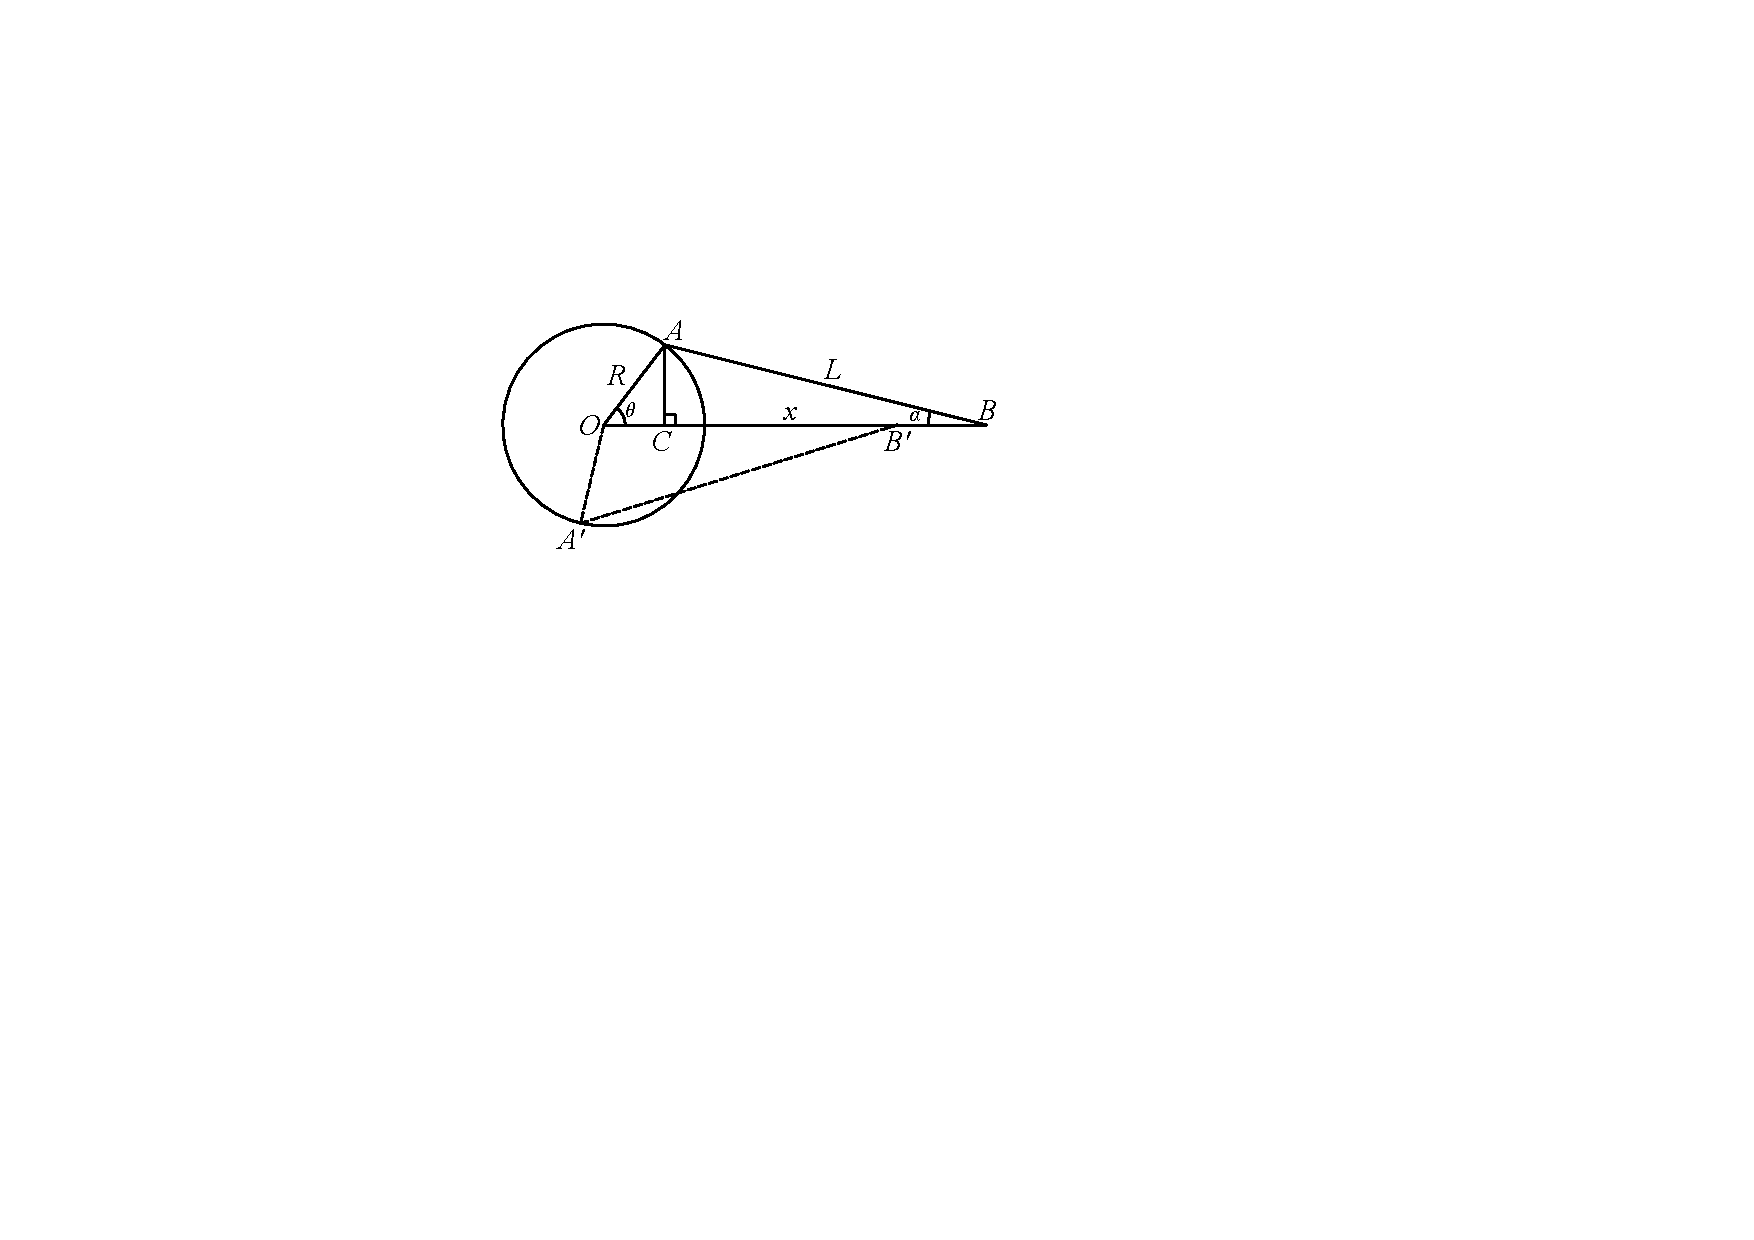
\includegraphics[width=0.5\linewidth]{曲轴-连杆机构}
\end{figure} \\
\textbf{方法一}\ 过$ A $点作$ OB $的垂线,垂足为$ C $,则
$ R\sin\theta=L\sin\alpha $,
\begin{align*}
x =R\cos\theta+L\cos\alpha=R\cos\theta+\sqrt{L^2-L^2\sin^2\alpha} 
=R\cos\theta+\sqrt{L^2-R^2\sin^2\theta}
\end{align*}
\textbf{方法二}\ 由余弦定理,$ L^2=R^2+x^2-2Rx\cos\theta $,
求解二次方程,抛弃掉一个解,也可以得到与方法一相同的结果。

$ R\cos\theta+\sqrt{L^2-R^2\sin^2\theta} $与$ R\cos\theta+L $
的函数图像对比如下,$ \dfrac{R}{L} $越小,两者的图像越接近。
\begin{figure}[h]
\centering
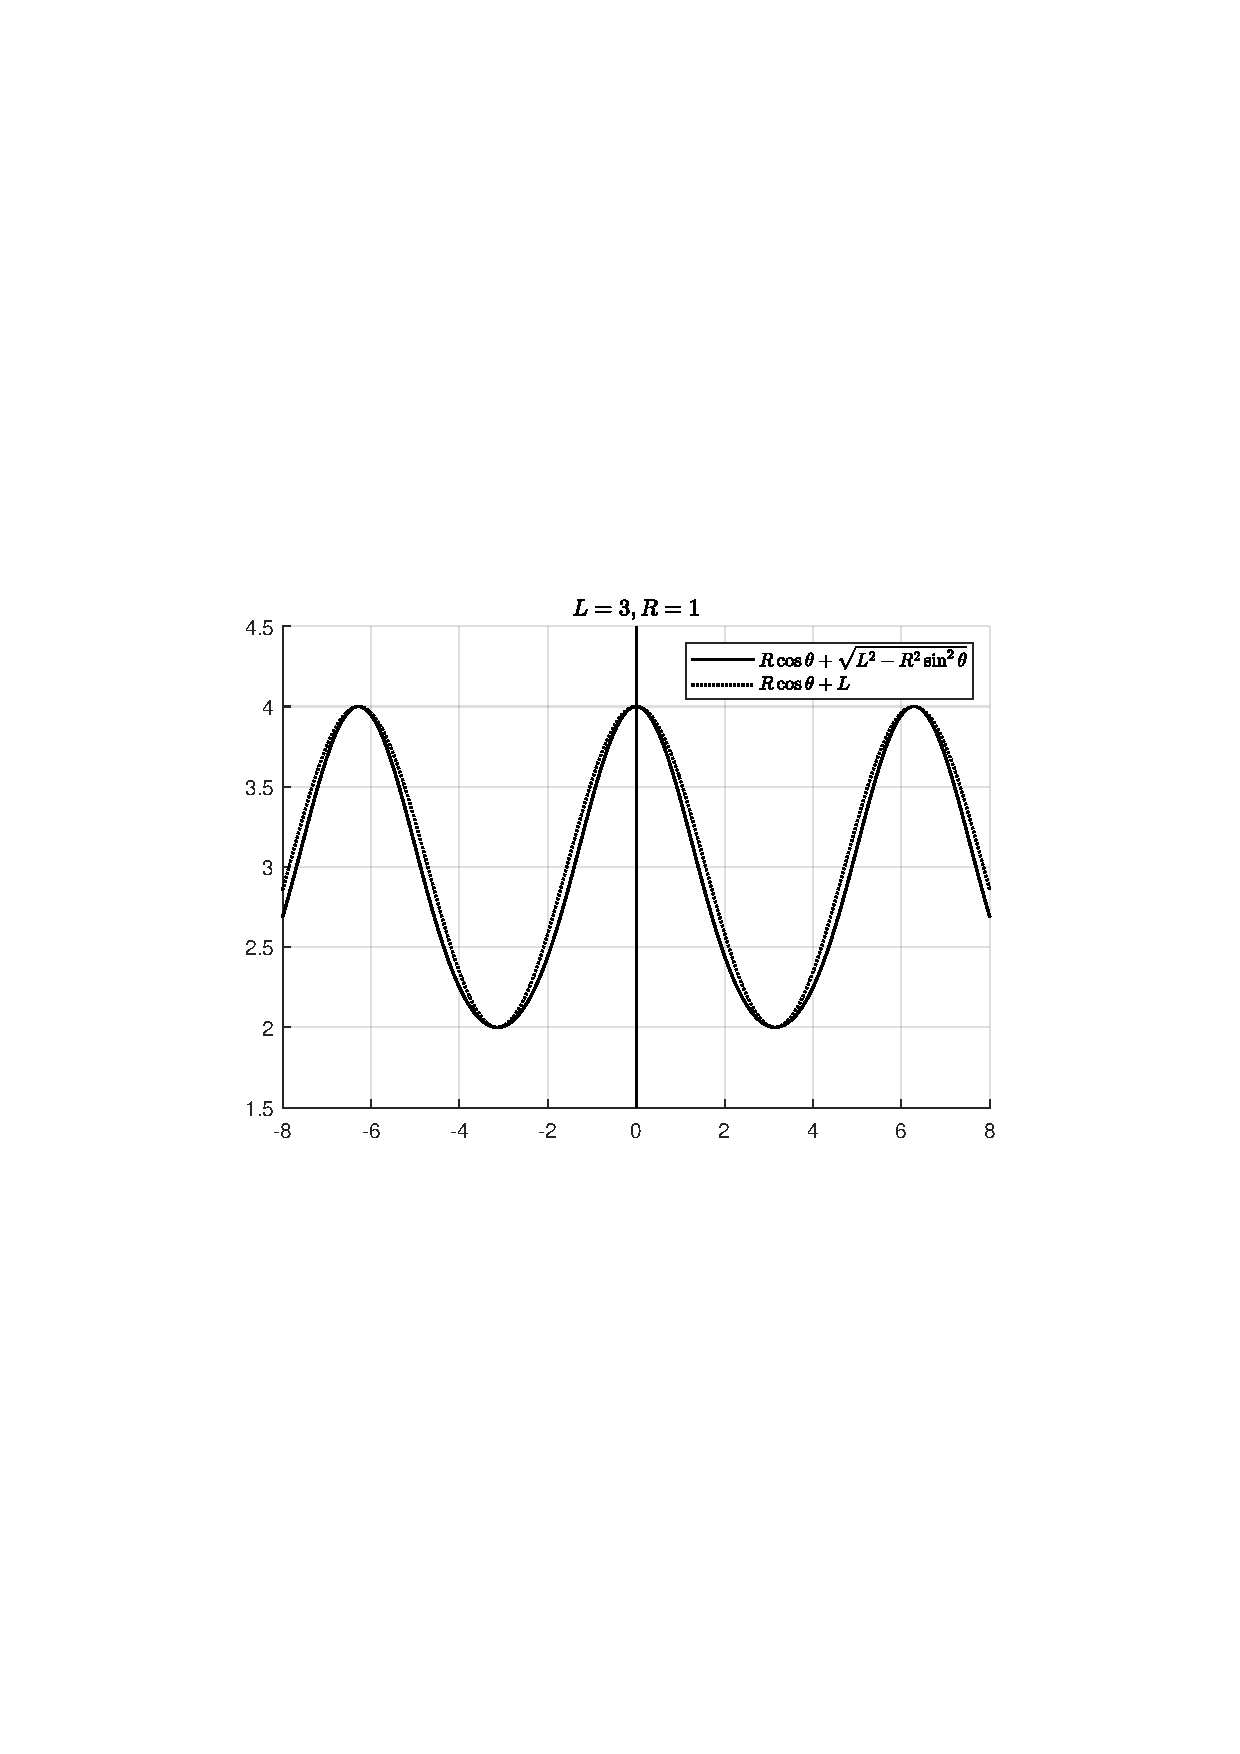
\includegraphics[width=0.5\linewidth]{曲轴-连杆机构函数图像}
\end{figure} 
\\
\textbf{变体}\ 如果$ B $点运动所在的直线(气缸中心轴)不经过$ O $点,
而与$ O $点的距离为$ d $,求$ x=|DB| $关于$ \theta $的关系式。
\begin{figure}[h]
\centering
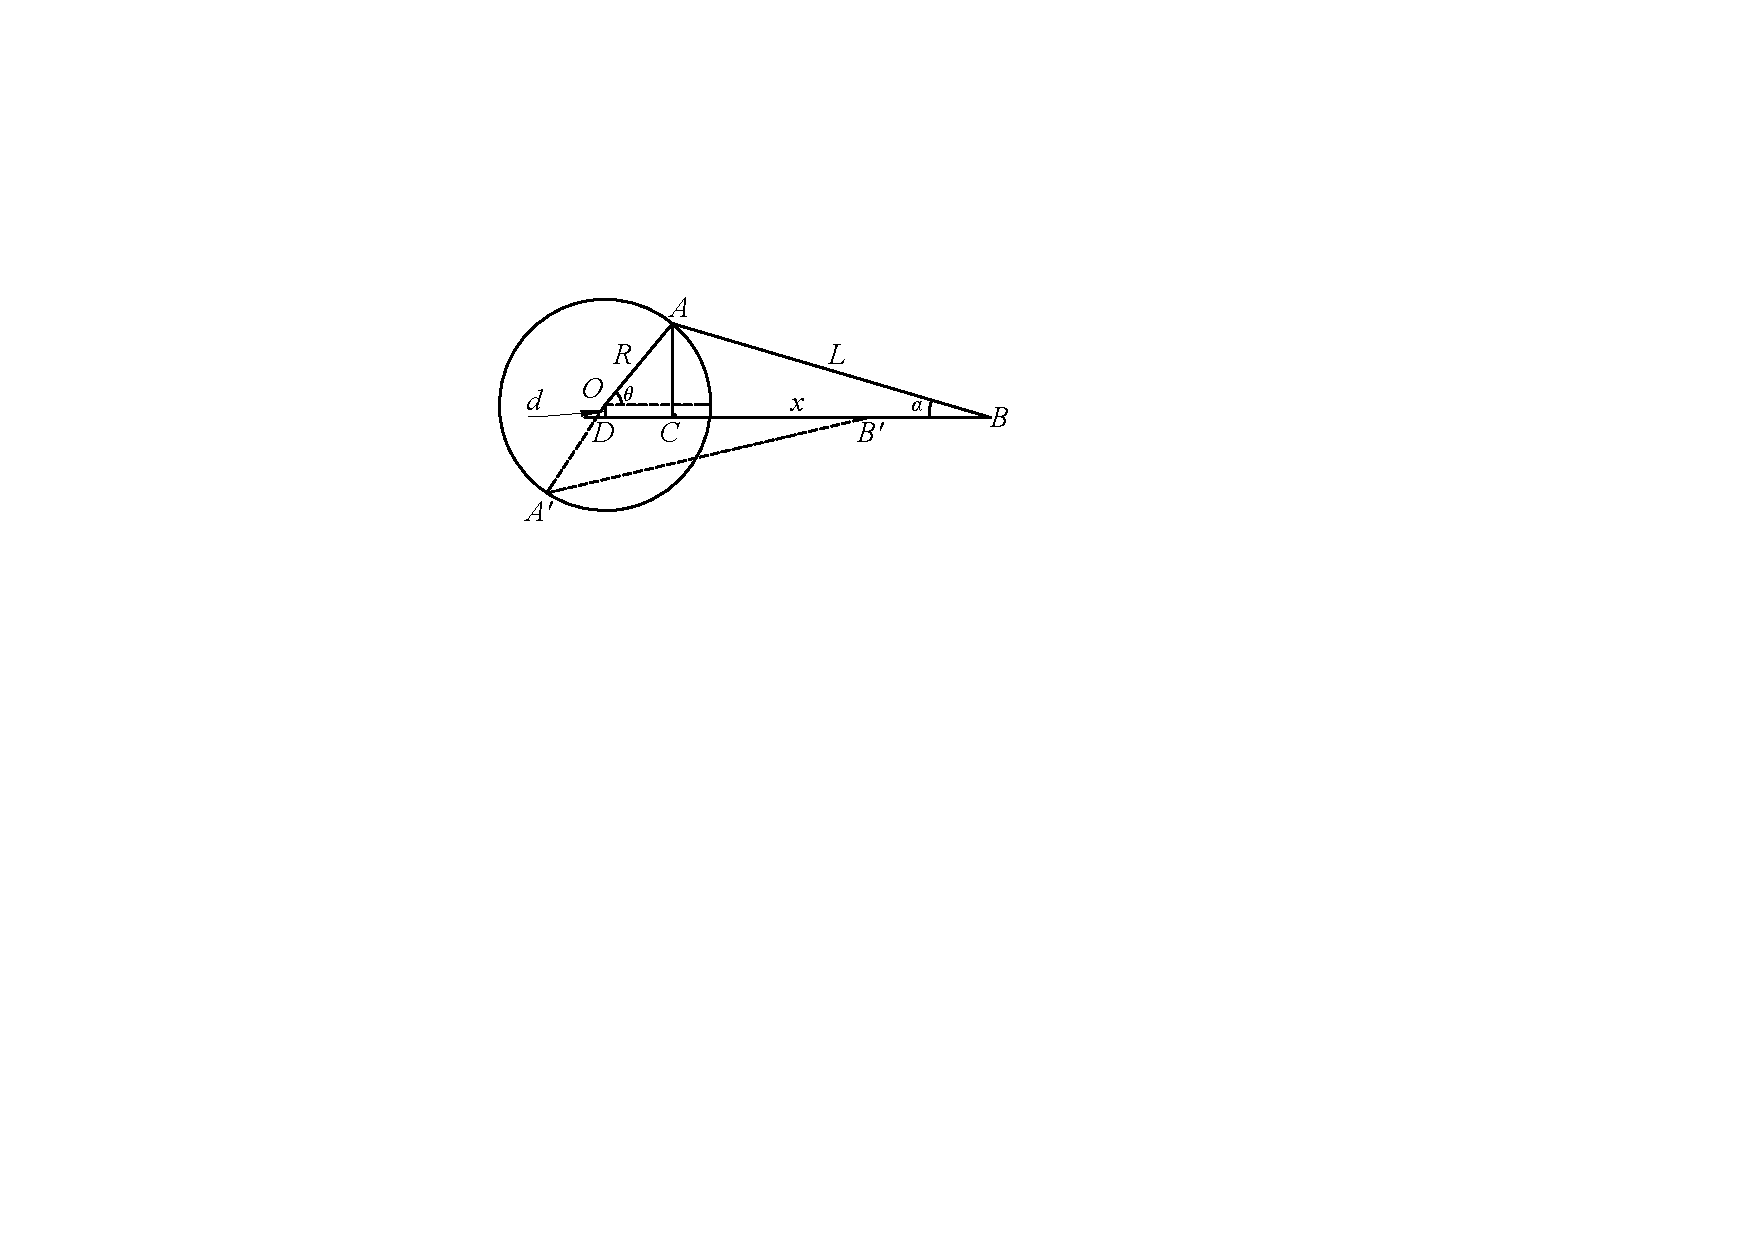
\includegraphics[width=0.5\linewidth]{曲轴-连杆机构-偏置}
\end{figure} \\
\textbf{解}\ $ R\sin\theta+d=L\sin\alpha $,
$ x=R\cos\theta+L\cos\alpha=R\cos\theta+\sqrt{L^2-(R\sin\theta+d)^2} $.

这种设计方案被称为“曲轴偏置”(分为正偏置与负偏置),正偏置的优点有
\footnote{$\diamond$ 顾丽,吴东兴,李波,等. 曲轴偏置和活塞销偏置对发动机摩擦损耗的影响研究[J]. 现代车用动力, 2018(3):3.\\
$\diamond$ 田丰果,睢娟. 曲轴偏置式发动机力学分析研究[J]. 数字技术与应用, 2009. \\
$\diamond$李永纯,张颖,袁海马.某型号发动机曲轴偏置分析.汽车工程师.(2014):44-46}:
在做功冲程中,连杆与气缸中心轴的夹角更小,
使发动机输出的扭矩和功率和热效率提高。同时可减小活塞环对气缸壁的正压力,从而减小摩擦力。

如果假设曲轴匀速旋转,即$ \theta=\omega t $,那么将$ x $对时间$ t $
求一阶导数和二阶导数,就能得到活塞往复运动的速度和加速度的变化规律。分析$ x $
的极大、极小值,就能得到活塞的行程,感兴趣的读者自行研究。

\item 设$ ABCD $是一个四边形,其中$ AD $边固定,另外三边可以运动
(但不会散开),设$ |AB|=l_1 $,$ |BC|=l_2 $,$ |CD|=l_3 $,
$ |DA|=l_4 $,假设已知$ \gamma $角,求$ \alpha,\ \beta $.
\begin{figure}[h]
\centering
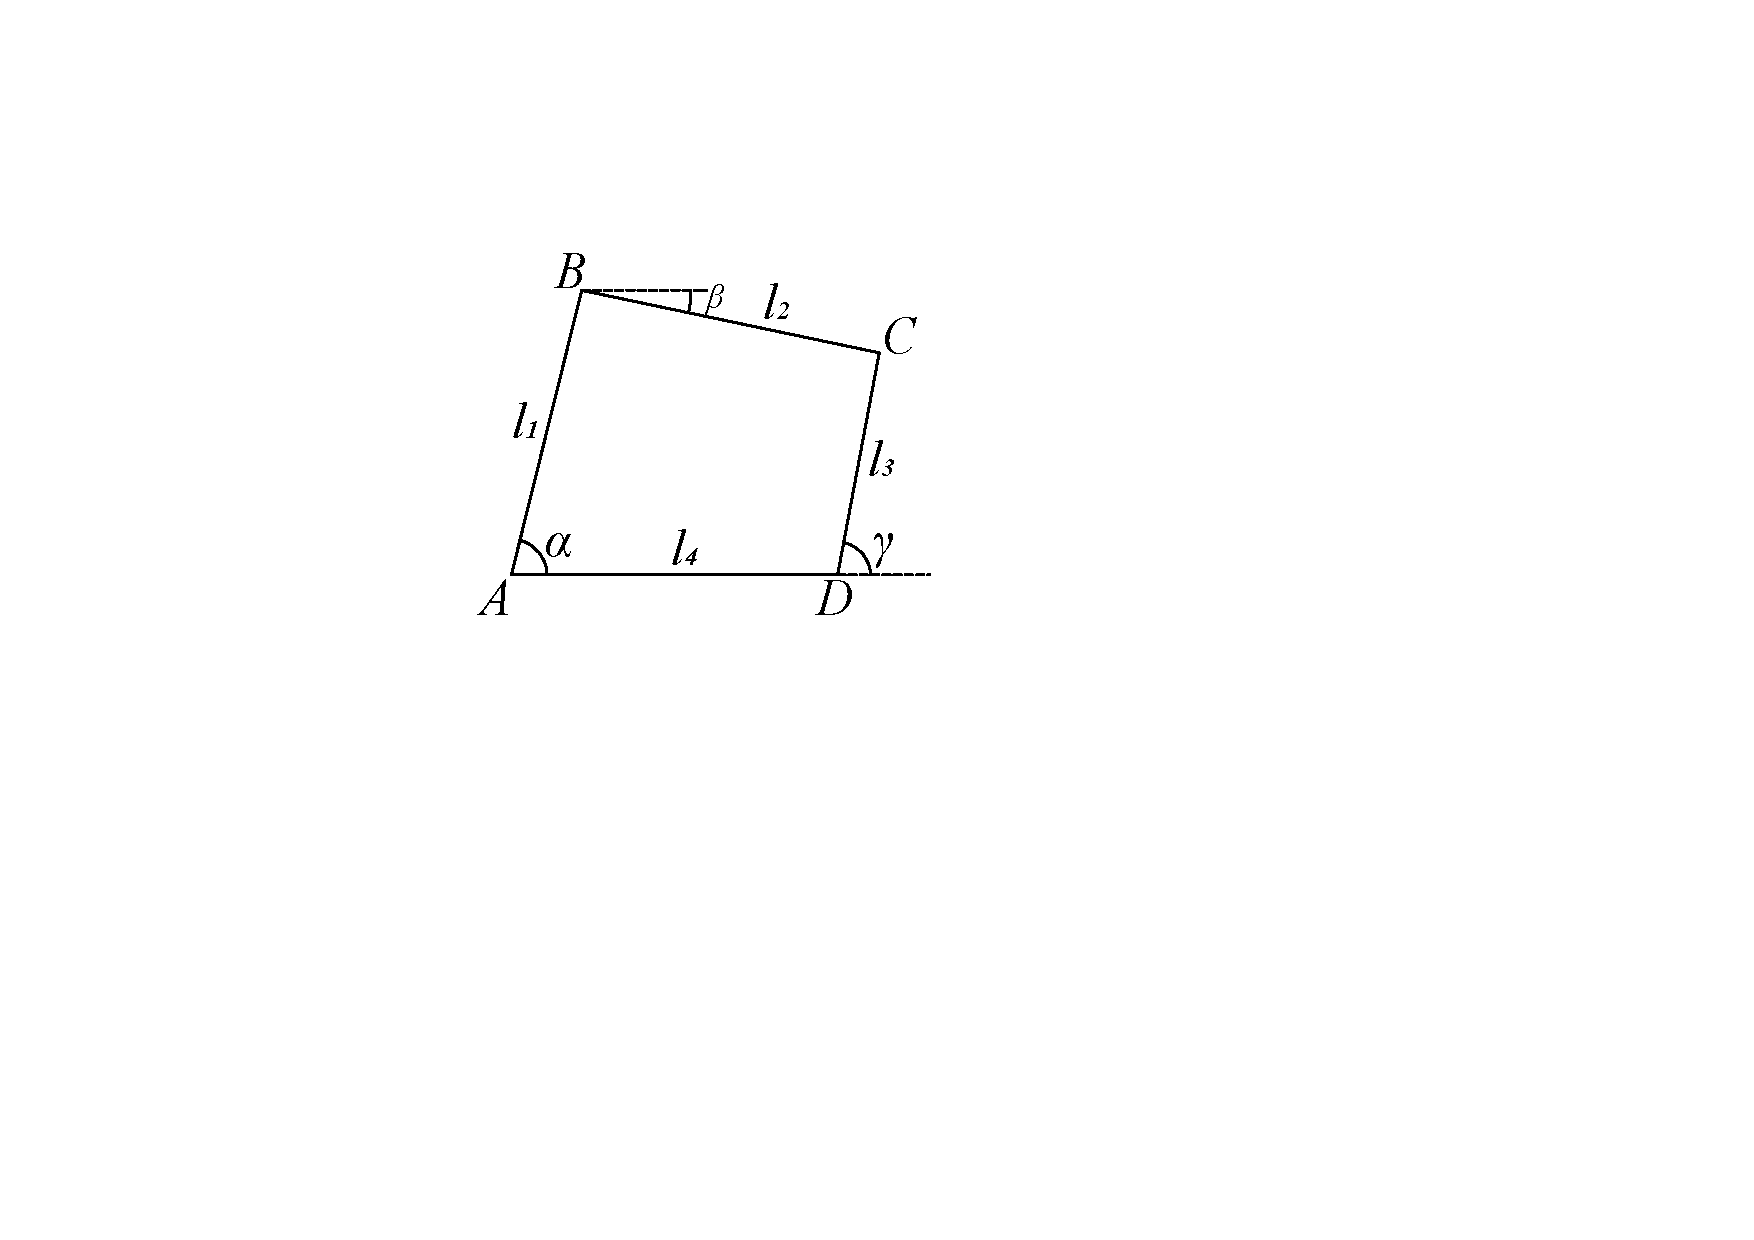
\includegraphics[width=0.3\linewidth]{四连杆机构}
\end{figure} \\
\textbf{解}\ 
\begin{align*}
\begin{cases}
    l_1\sin\alpha +l_2\sin\beta=l_3\sin\gamma \\
    l_1\cos\alpha +l_2\cos\beta=l_4+l_3\cos\gamma 
\end{cases}
\end{align*}
以上两式平方后相加可得:
\begin{gather*}
l_1^2+l_2^2+2l_1l_2\cos(\alpha-\beta)=
l_3^2+l_4^2+2l_3l_4\cos\gamma =|AC|^2 \\
\alpha-\beta=\arccos\frac{l_3^2+l_4^2+2l_3l_4\cos\gamma-
    l_1^2-l_2^2}{2l_2l_2}
\end{gather*}
这样就相当于消去了一个变量,剩余的计算过程比较容易,在此略去。

本题中的可变形四边形是生活中的四连杆机构的抽象,
四连杆机构在很多机械设备中都有应用。
比如汽车转向系统中最常见的的阿克曼转向系统,
就是一个四连杆机构(其中有两根杆的长度相等),
作用是让汽车在转向时,弯道内侧车轮的偏转角大于外侧车轮,
尽量让内侧车轮和外侧车轮具有共同的转向中心,减少轮胎磨损。

\item 假设你偶遇了迪迦奥特曼,想测量他的身高。如下图所示,你位于左侧大楼
的$ A $点,大楼$ CD $对迪迦腿部有遮挡。你手上只有一台激光测距仪,
此仪器只能测量距离,无法测量角度。请设计一种测量方案,
测出迪迦当前站姿的身高$ EF $(不必考虑两腿没有并拢)。
\begin{figure}[h]
    \centering
    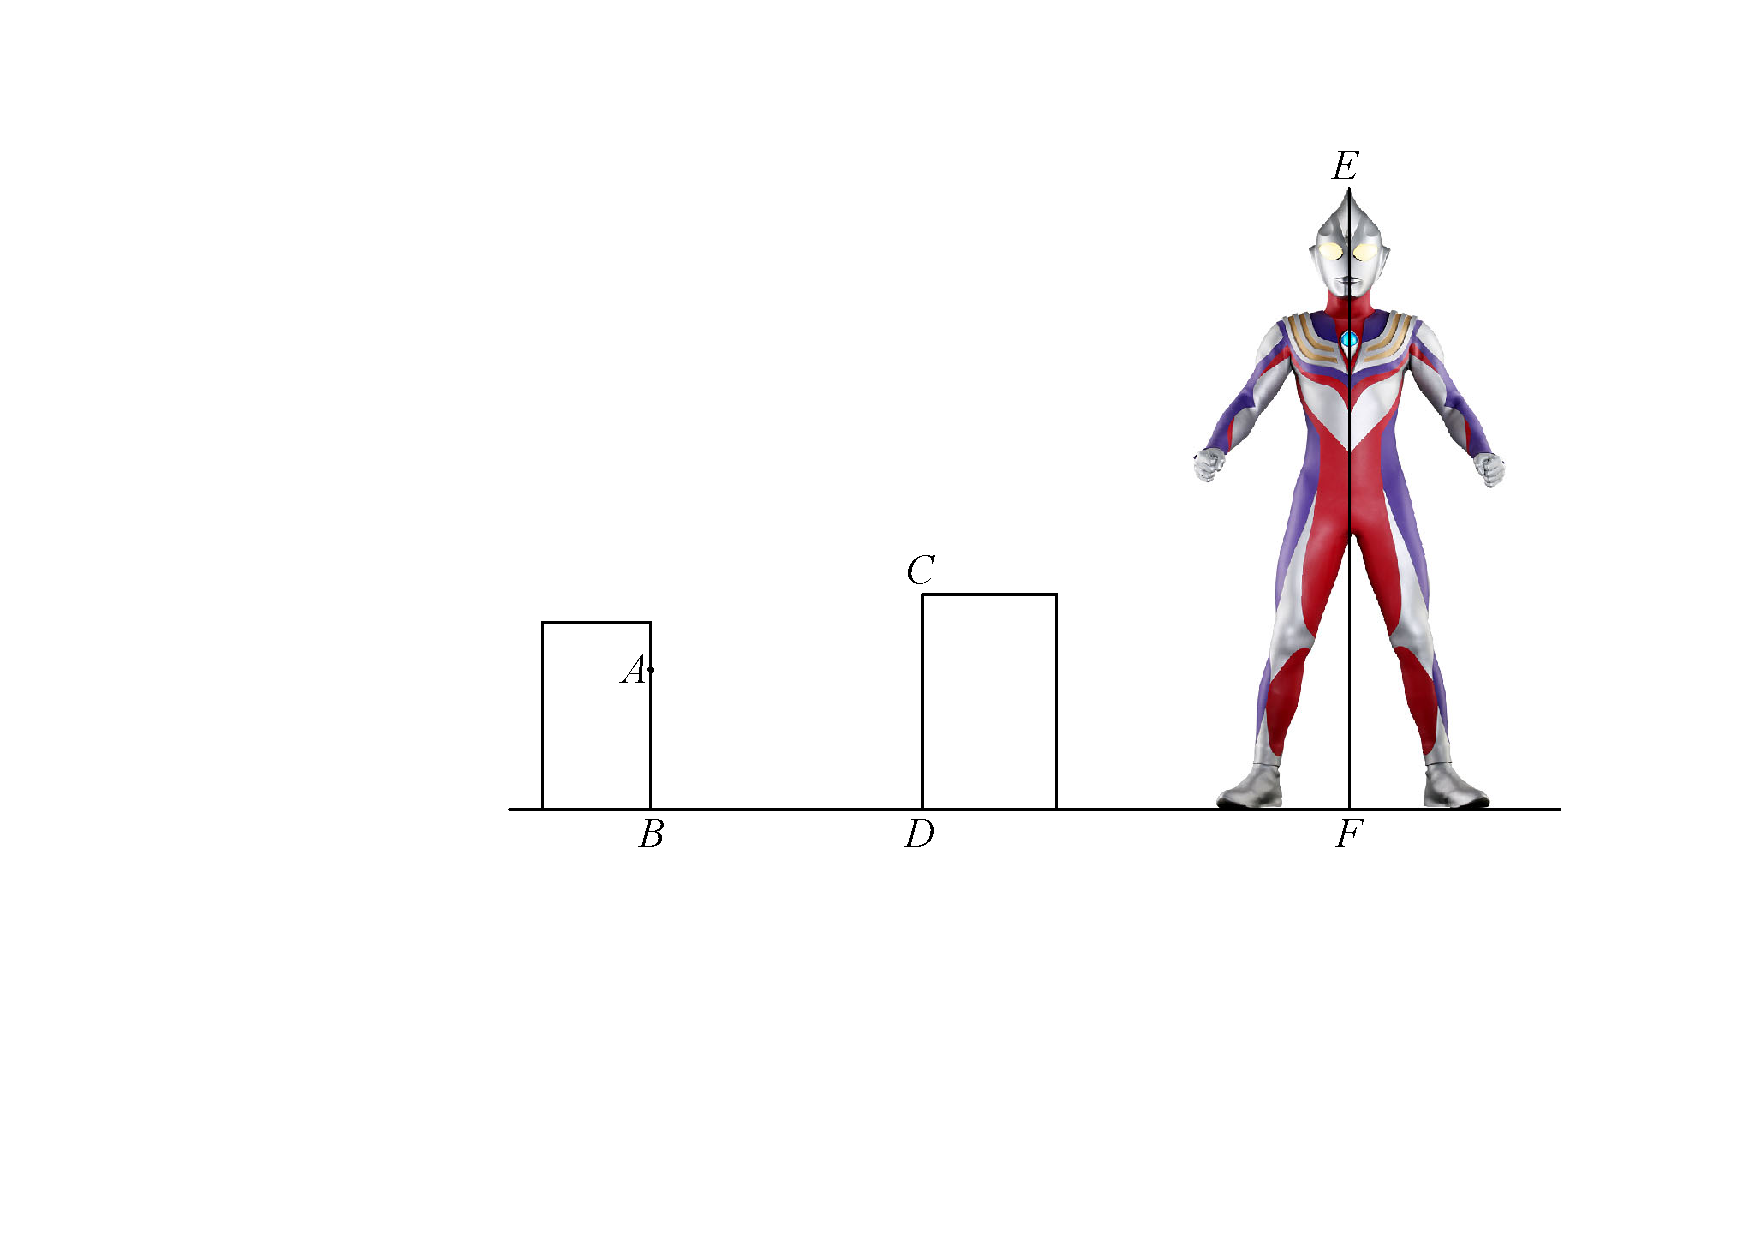
\includegraphics[width=0.6\linewidth]{迪迦身高计算(无测量方案)}
\end{figure} \\
\textbf{解}\ 测量方案如下:
\begin{figure}[h]
    \centering
    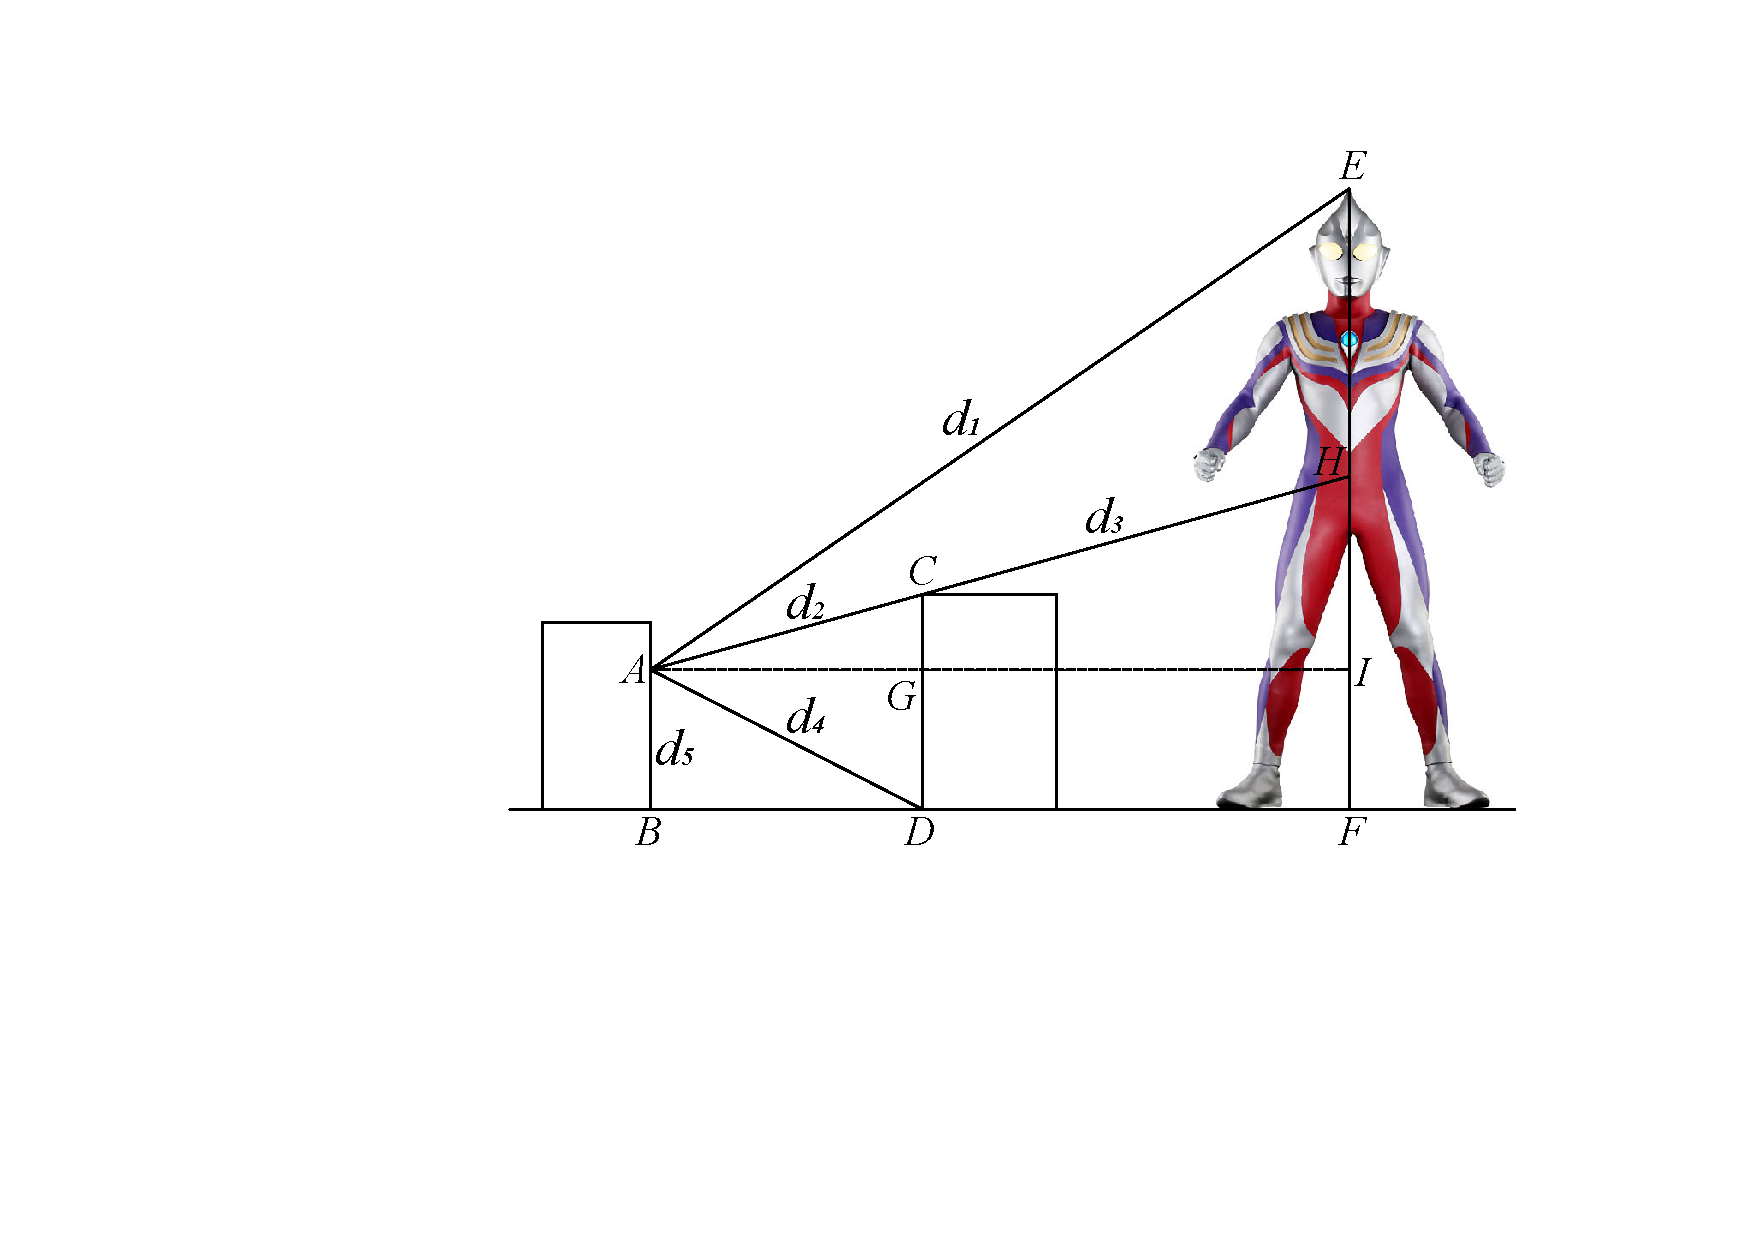
\includegraphics[width=0.6\linewidth]{迪迦身高计算(有辅助线)}
\end{figure} \\
测出$ |AE|=d_1 $, $ |AC|=d_2 $, $ |AH|=d_3 $(注意不是$ |CH|=d_3 $),
$ |AD|=d_4 $, $ |AB|=d_5 $,即可得到$ EF $.
但因为$ H $点是$ AC $延长线与$ EF $的交点,该点位于迪迦的体内,
激光测距仪无法测量。所以需要观测者沿垂直于纸面的方向,
平移测距仪的位置,以迪迦腹部表面的点来代替体内的点,进而测出$ |AH| $.
计算如下:过$ A $点作水平线,交$ CD $于$ G $点,交$ EF $于$ I $点,
则$ |AG|=|BD|=\sqrt{d_4^2-d_5^2} $.因为$ \Delta AGC \backsim \Delta AIH $,
所以
\begin{gather*}
    \dfrac{|AC|}{|AH|}=\dfrac{d_2}{d_3}=\dfrac{|AG|}{|AI|},\q  |AI|=\dfrac{d_3\sqrt{d_4^2-d_5^2} }{d_2},\q |EI|=\sqrt{d_1^2-|AI|^2}
\end{gather*}
最终有
\begin{gather*}
    |EF|=|EI|+|IF|=\sqrt{d_1^2-\frac{d_3^2(d_4^2-d_5^2)}{d_2^2}}+d_5
\end{gather*}
\textbf{注1}\ 以上方案也存在一些不足,如果大楼$ CD $太矮或者$ A $点位置太高,
那么$ H $点将位于迪迦的两腿之间,是一个悬空的点,从而无法测距。
当然,如果把迪迦换成一栋长方体形的大楼,那就不存在这个麻烦了。\\
\textbf{注2}\ 假如还可以测量角度,那么是否可以避免“要测量到悬空的点的距离”的困难
\footnote{可以避免。不测$ |AH| $,改为测量$ \angle EAD $即可,因为$ \angle 
    GAD=\arcsin\dfrac{d_5}{d_4} $是已知的,那么$ \angle EAG=\angle EAD-\angle 
    GAD $,$ |EI|=d_1\sin\angle EAG $. }?\\
\textbf{注3}\ 假如没有大楼$ CD $的遮挡(但不能测量角度),可以测量到$ F $点的距离,
又该如何测量身高\footnote{设$ |AF|=d_6 $,再利用$ d_1,d_5 $即可,
    $ |EF|=\sqrt{d_1^2-(d_6^2-d_5^2)}+d_5 $. }?

\end{enumerate}
%~\newpage

\section{习题}
\begin{enumerate}[label={\textbf{\arabic*.}},leftmargin=
    \inteval{\myenumleftmargin}pt]
\item 在$ \Delta ABC $中,已知$ a^2+b^2+c^2=2\sqrt{3}bc\sin A $,求$ B $的大小。

\item $ \vec{a}=(4,t),\ \vec{b}=\left(t,\dfrac{5}{3}\right) $,若
$ \vec{a}//\vec{b} $,则$ t= $\underline{\hspace{2cm}};
若$ \vec{a},\vec{b} $夹角为$ \dfrac{\pi}{4} $,
则$ t= $\underline{\hspace{2cm}}.

\item 平面直角坐标系中有4点,它们的坐标分别为$ A(3,4),B(6,0),C(7,2),D(4,6) $,
求四边形$ ABCD $的面积。

\item 在$ \Delta ABC $中,$ \sin^2A\leq\sin^2B+\sin^2C-
\sin B\sin C $,求$ A $的取值范围。

\item 证明恒等式(\ref{三角恒等式2})$ \sim $ (\ref{三角恒等式-最后}).

\item 求证:在$ \Delta ABC $中,\\ $ \sin (nA) +\sin (nB) +\sin (nC)=
\begin{cases}
    - 4\sin\left(\dfrac{nA}{2}\right)\sin\left(\dfrac{nB}{2}\right)
    \sin\left(\dfrac{nC}{2}\right),& n=4k \\
    4\cos\left(\dfrac{nA}{2}\right)\cos\left(\dfrac{nB}{2}\right)
    \cos\left(\dfrac{nC}{2}\right),& n=4k+1 \\
    4\sin\left(\dfrac{nA}{2}\right)\sin\left(\dfrac{nB}{2}\right)
    \sin\left(\dfrac{nC}{2}\right),& n=4k+2 \\
    - 4\cos\left(\dfrac{nA}{2}\right)\cos\left(\dfrac{nB}{2}\right)
    \cos\left(\dfrac{nC}{2}\right),& n=4k+3
\end{cases} $

\item 求证:在锐角$ \Delta ABC $中,\\
(I) $ \sin A +\sin B +\sin C > \dfrac{4}{3} (\cos A +\cos B +\cos C) $. \\
(II) $ \tan^2 A+\tan^2 B +\tan^2 C \geq 9 $.

\item 正实数$ x,y,z,a,b,c $满足
$ \begin{cases} 
    x^2+xy+y^2= a^2 \\
    y^2+yz+z^2= b^2 \\
    z^2+zx+x^2= c^2  
\end{cases} $,\\
(I) 若$ a^2=6,\ b^2=7,\ c^2=8 $,
求$ xy+yz+zx,\ x+y+z $以及$x,y,z$. \\
(II) 若$a^2+c^2=2b^2$,求证:$ y+z=2x $.

\item 
$\begin{cases}
    x^2+y=a \\
    y^2+z=b \\
    z^2+x=c 
\end{cases}$,其中$x,y,z$是未知数,$a,b,c$是常数,
通过消元法求出$x$所满足的8次方程。

\item 在$ \Delta ABC $中,已知$ AB=7,AC=8,BC=9 $,那么它的面积为\underline{
    \hspace{1cm}},内切圆半径为\underline{\hspace{1cm}},外接圆半径为\underline{
    \hspace{1cm}},$ \vec{AB}\cdot \vec{AC}
=$\underline{\hspace{1cm}},$ BC $边的中点为$ D $,$ AD $
的长度为\underline{\hspace{1cm}}.$ I $是它的内心,$ O $是它的外心,
则$ \vec{AO}\cdot\vec{BC} = $\underline{\hspace{2cm}},
$ \vec{AI}\cdot\vec{BC}= $\underline{\hspace{2cm}}.

\item 已知正方形$ ABCD $的边长为1.当每个$ \lambda_i(i=1,2,3,4,5,6) $取遍
$ \pm 1 $时,求\\ $|\lambda_1\vec{AB}+\lambda_2\vec{BC}+\lambda_3
\vec{CD}+\lambda_4\vec{DA}+\lambda_5 \vec{AC}+\lambda_6\vec{BD}| 
$的最小值和最大值.

\item \label{以AB为直径作圆习题} 下图中,$ AB=4,BC \perp AB $,以$ AB $为直径作一个圆,$ BD $是$ \angle ABC $的平分线,$ P $是$ BD $上任意一点,$ EF $是圆$ O $的任意一条直径,求$ \vec{PE}\cdot \vec{PF} $的最小值。
\begin{figure}[h]
    \centering
    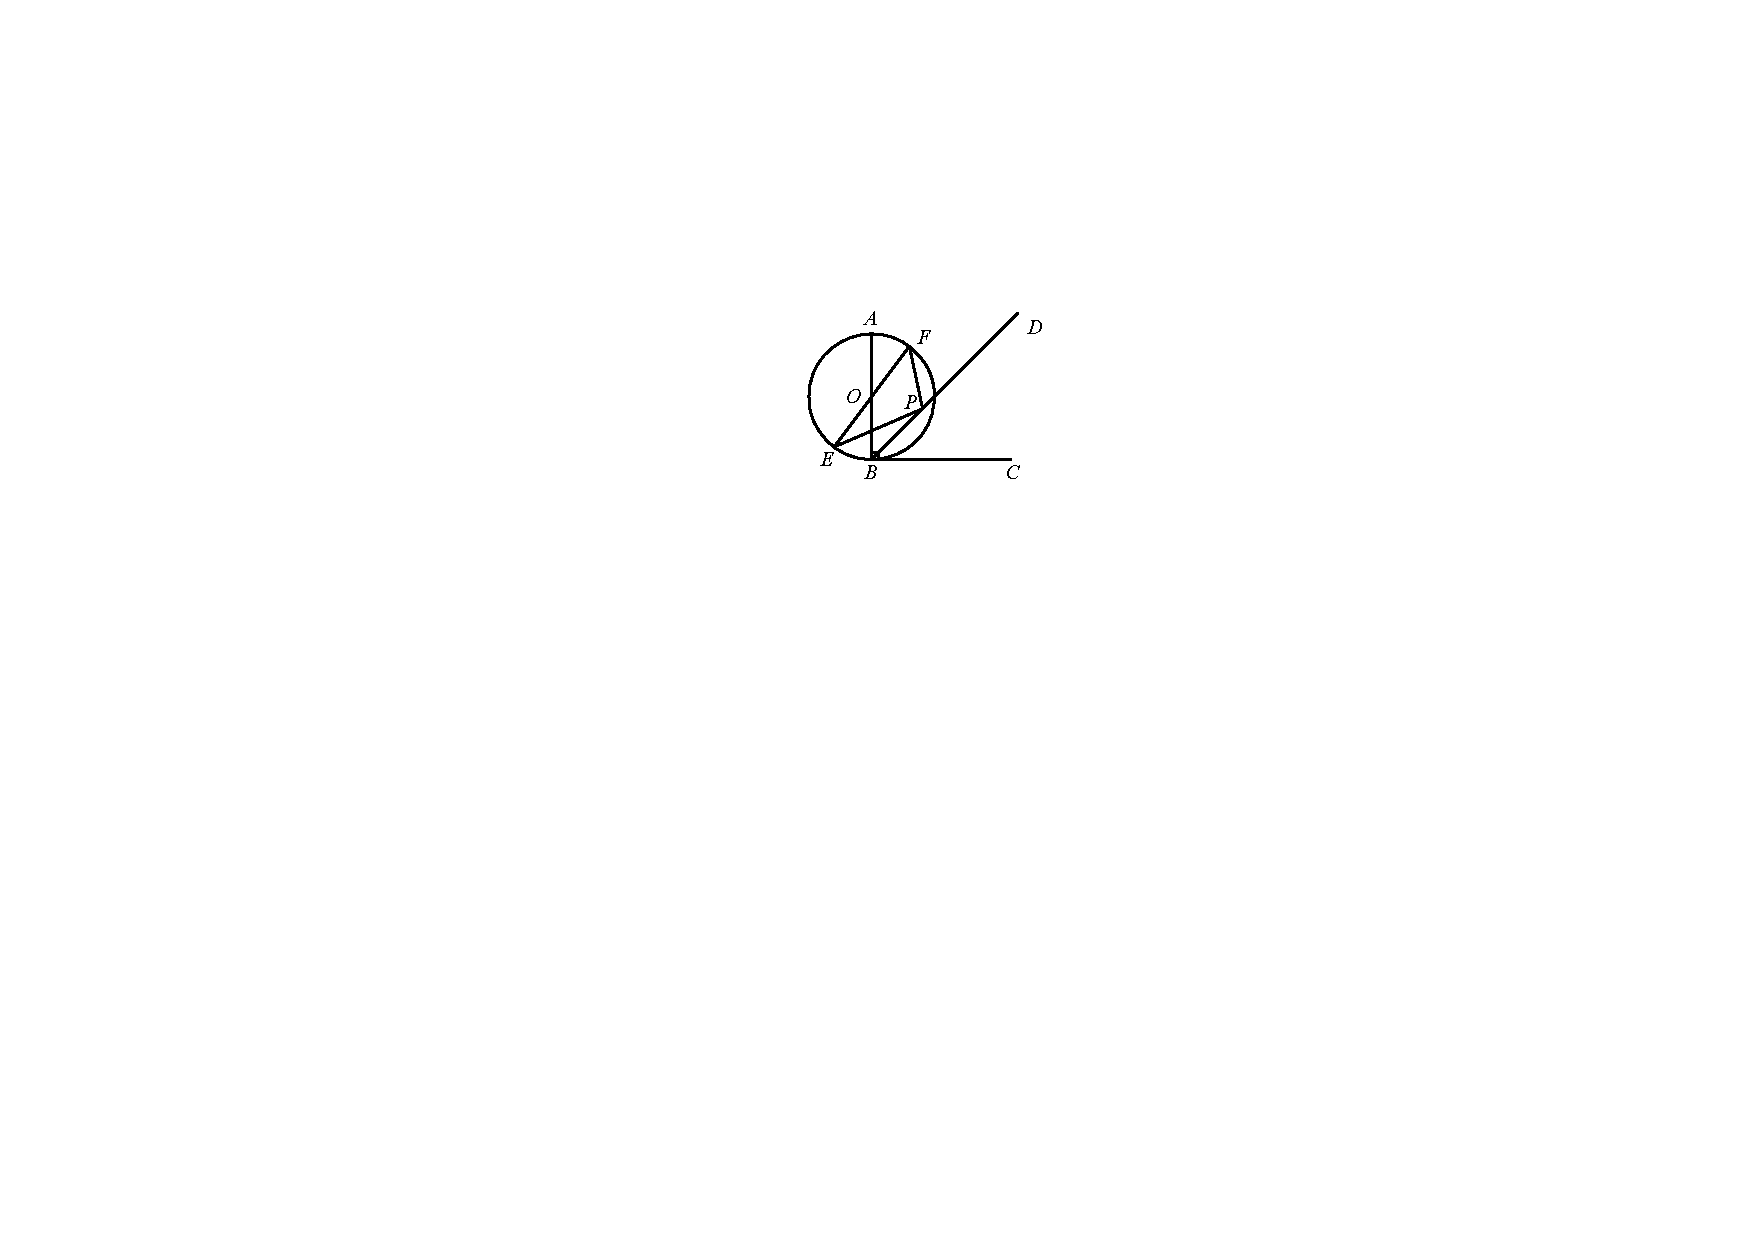
\includegraphics[width=0.25\linewidth]{PAxPB最值问题}
    \caption*{\ref{以AB为直径作圆习题}题图}
\end{figure}

\item \label{AE=4_5AB+1_5AC习题}在$ \Delta ABC $中,已知$ \vec{AE}=\dfrac{4}{5}
\vec{AB}+\dfrac{1}{5}\vec{AC},\ \vec{BD}=
\dfrac{1}{3}\vec{BC}+\dfrac{2}{3}\vec{BA} $,
$ AE $与$ BD $交于点$ F $,设$ \vec{BF}=\lambda 
\vec{BD} $,求$ \lambda $. 
\begin{figure}[h]
    \centering
    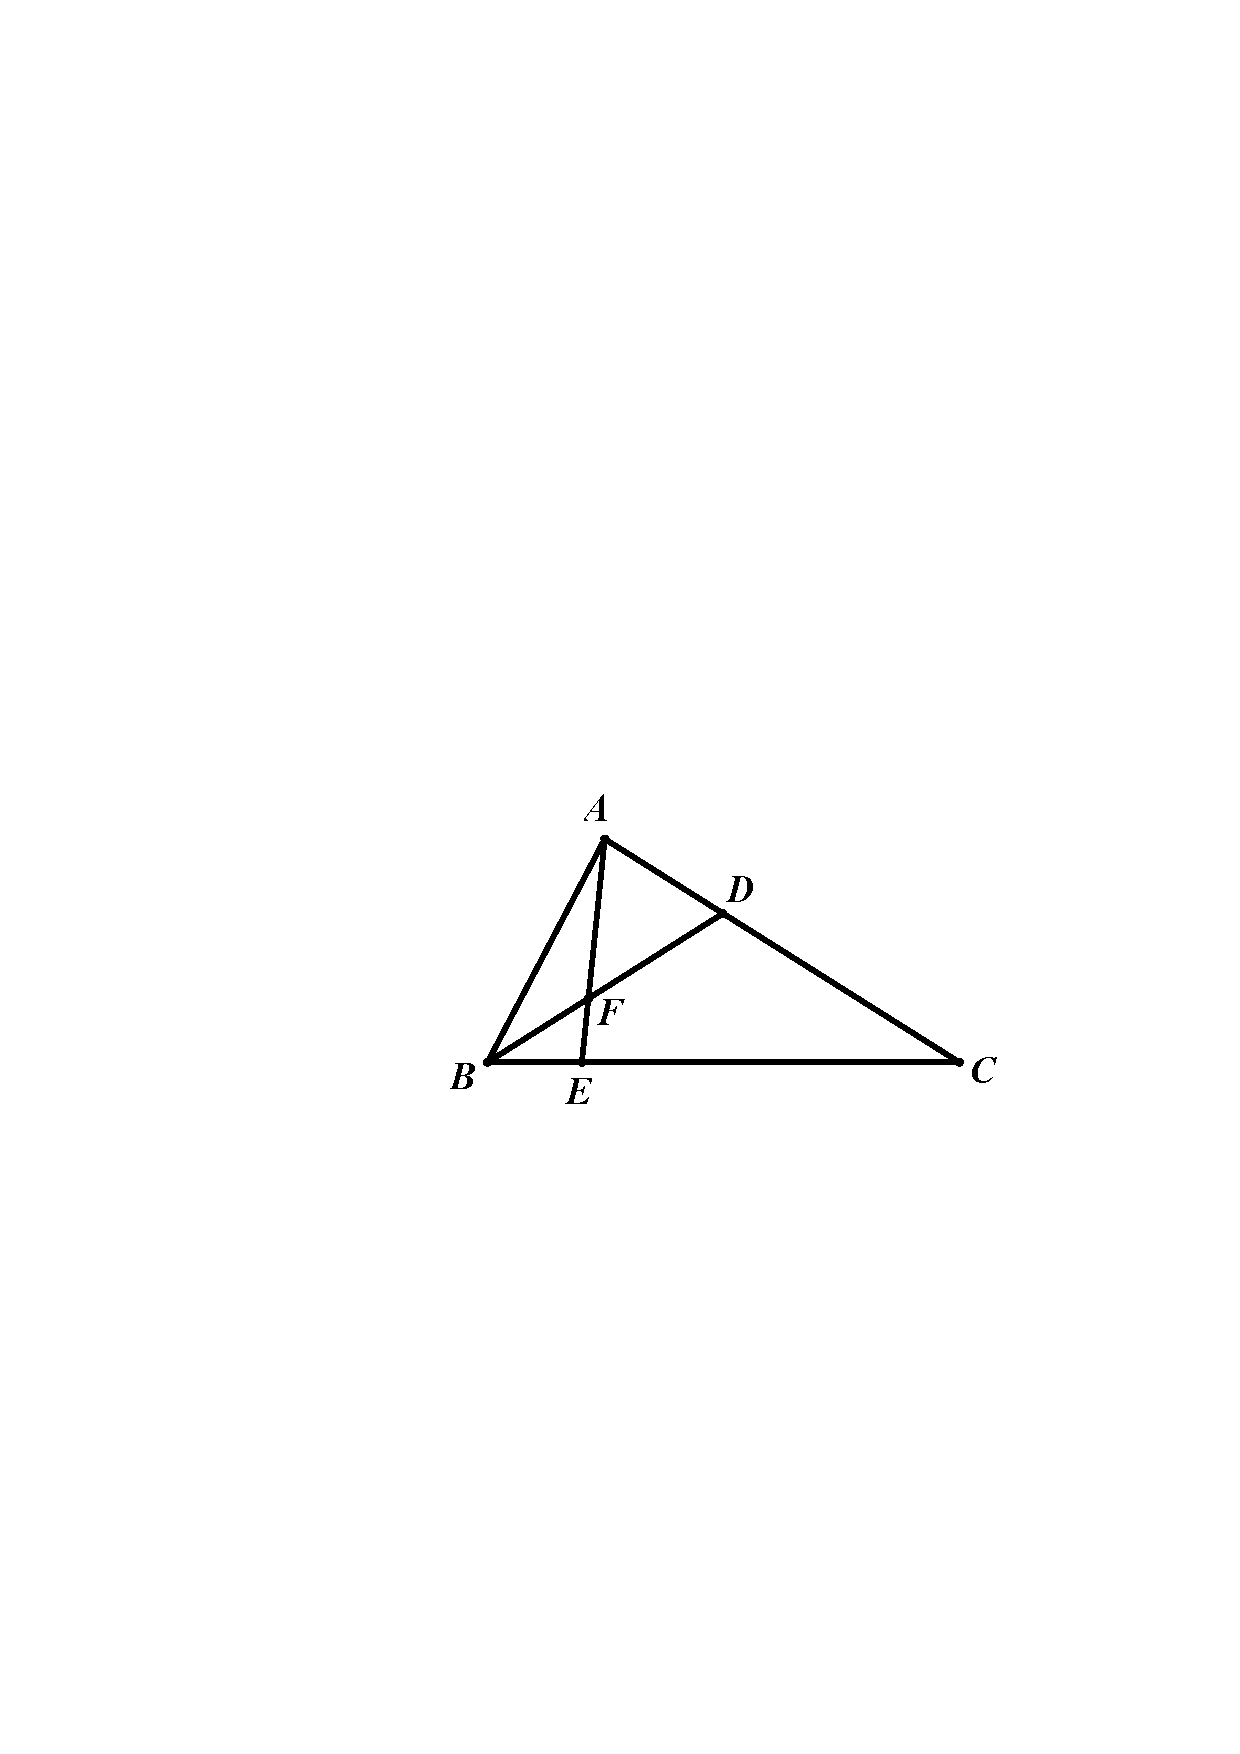
\includegraphics[width=0.3\linewidth]{长度占比习题2}
    \caption*{\ref{AE=4_5AB+1_5AC习题}题图}
\end{figure}

\item 设$ H $为$ \Delta ABC $的垂心,且有$ \vec{AH}=
\dfrac{1}{2}\vec{AB}+\dfrac{3}{10}\vec{AC} $,
求$ \cos \angle BAC $. 

\item 在$ \Delta ABC $中,$ D $是$ BC $边上一点,且$ \vec{BD}=
\dfrac{1}{5}\vec{BC} $. $ E $是$ AD $上一点,$ \vec{AE} =
\dfrac{2}{3}\vec{AD} $. 过$ E $点的直线与$ AB,AC $所在的直线分别交于
$ M,N $两点,设$ \vec{AM}=x\vec{AB},\vec{AN}=
y\vec{AC} $,且$ x>0,y>0 $. \\
(1)求$ \dfrac{8}{x}+\dfrac{2}{y} $的值;\q  (2)求$ xy $的最小值。
\begin{figure}[!htbp]
    \centering
    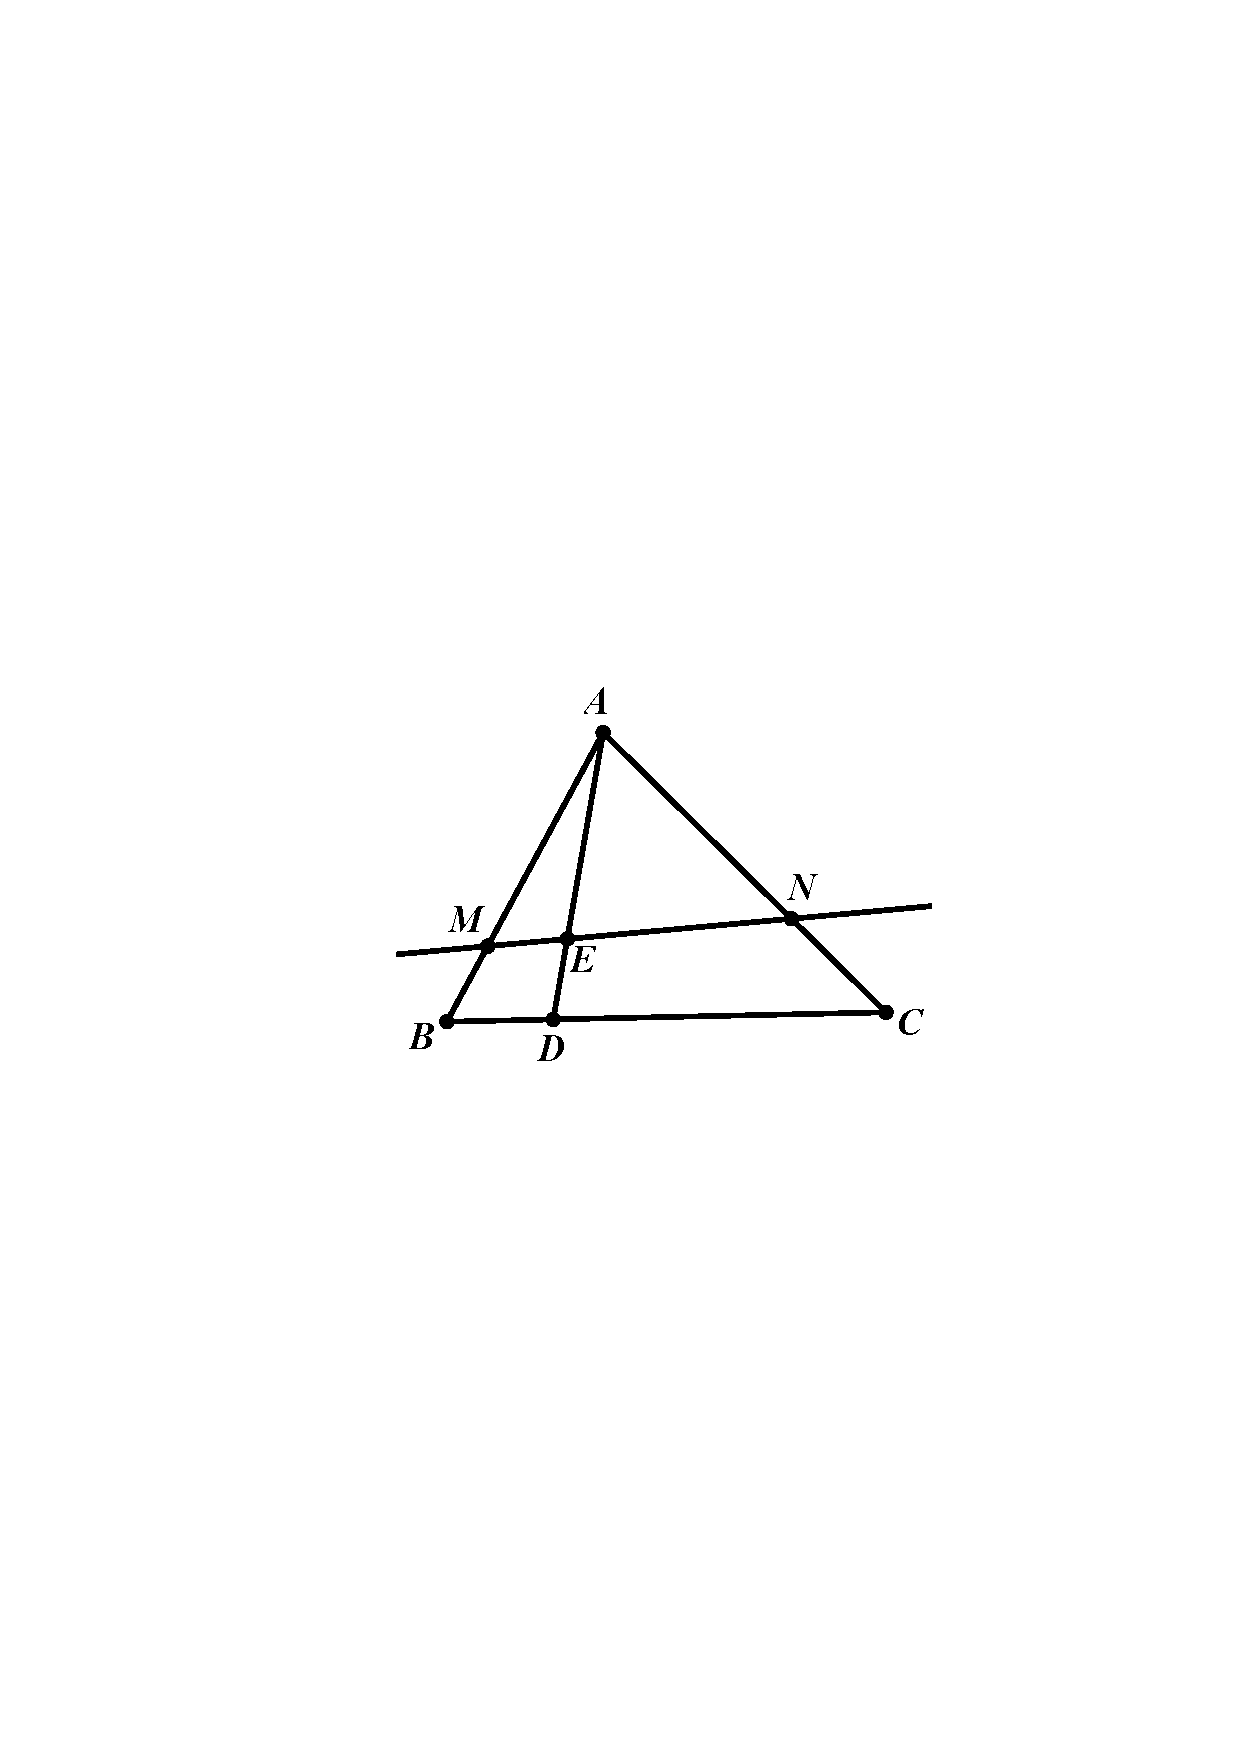
\includegraphics[width=0.3\linewidth]{系数倒数相加为定值}
\end{figure} 

\item 求证:在任意三角形中,小角的角平分线段比大角的角平分线段更长。
(“角平分线段”是指角平分线从顶点到对边的部分。)

\end{enumerate}

\section{习题答案}
\begin{enumerate}[label={\textbf{\arabic*.}},leftmargin=
    \inteval{\myenumleftmargin}pt]
\item 
根据外森比克不等式,$ \Delta ABC $为等边三角形,$ B=\dfrac{\pi}{3} $. 

\item 
$ \pm\dfrac{2\sqrt{15}}{3} $,1或$ \dfrac{20}{3} $,不能取负数,负数对应$ \dfrac{3\pi}{4} $. 

\item 
$ \vec{AB}=\vec{DC}=(3,-4),
\vec{AD}=\vec{BC}=(1,2),\ S=|-4-6|=10 $. 也可以使用
\eqref{多边形面积公式}式,注意按顺时针或者逆时针方向排列顶点,
而不要不假思索地按题目给出的顶点顺序。

\item 利用正弦定理“角化边”:$ a^2\leq b^2+c^2-bc $,所以
\begin{gather*}
    \cos A=\dfrac{b^2+c^2-a^2}{2bc}\geq \dfrac{1}{2},
    \q 0<A\leq \dfrac{\pi}{3}
\end{gather*}
\textbf{方法二}\ 利用$ \sin A=\sin(B+C)=\sin B\cos C+\cos B\sin C $,
\begin{gather*}
    \sin^2B\cos^2C+2\sin B\cos B\sin C\cos C+\sin^2C\cos^2B
    \leq \sin^2B+\sin^2C-\sin B\sin C \\
    \sin B\sin C(2\cos B\cos C+1)\leq 2\sin^2B \sin^2C \\
    \cos(B+C)\leq -\dfrac{1}{2} 
\end{gather*}
剩余略。此法计算量较大,不推荐。

\item 略

\item 略

\item (1) 当$ x\in\Big(0,\dfrac{\pi}{2}\Big) $时,
$ \sin x>\dfrac{2}{\pi}x $,所以
\begin{gather*}
    \sin A +\sin B +\sin C>\dfrac{2}{\pi}(A+B+C)=2
\end{gather*}
根据(\ref{三个余弦和不等式-小于})式,$ \cos A +\cos B +\cos C\leq \dfrac{3}{2} $,
所以,
\begin{gather*}
    \sin A +\sin B +\sin C>2 \geq \dfrac{4}{3} (\cos A +\cos B +\cos C)
\end{gather*}
事实上有更强的不等式:
\begin{gather*}
    \sin A +\sin B +\sin C>\Big(1+\dfrac{\sqrt{2}}{2}\Big)(\cos A +\cos B +\cos C)
\end{gather*}
只有当三角形为等腰直角三角形时,上面的不等号才能变成等号;对于钝角三角形,上式不成立。\\
(2)
\begin{align*}
    &\ \tan^2 A+\tan^2 B +\tan^2 C \\
    \geq &\ \dfrac{1}{3}(\tan A+\tan B +\tan C)^2\q (\text{柯西不等式}) \\
    \geq &\ \dfrac{1}{3}\Big(3\tan\dfrac{A+B+C}{3}\Big)^2\q 
    (\text{正切函数的凹凸性}) \\
    = &\ 9
\end{align*}
$ A=B=C=\dfrac{\pi}{3} $时,等号成立。

\item  % FermatPoint_6_7_8.m
(I) $ a^2=6,b^2=7,c^2=8 $,\\
$ u=a^4+b^4+c^4=149,\ v=a^2b^2+b^2c^2+c^2a^2=146 ,
\ w=a^2+b^2+c^2=21 $,\\
$ \sigma_2=xy+yz+zx=\sqrt{\dfrac{-u+2v}{3}}=
\sqrt{\dfrac{143}{3}}=6.904105\cdots $, \\
$s_2=\dfrac{1}{2}\left(w-\sqrt{\dfrac{-u+2v}{3}}\right)
=\dfrac{1}{2}\left(21-\sqrt{\dfrac{143}{3}}\right)
=7.047947\cdots$,\\
$ s_1=x+y+z=\sqrt{\dfrac{1}{2}[w+\sqrt{3(-u+2v)}]}=
\sqrt{\dfrac{1}{2}(21+\sqrt{429})}=4.566854\cdots $. 
\begin{gather*}
\begin{cases}
    x=\dfrac{1}{3}\left(s_1+\dfrac{a^2+c^2-2b^2}{s_1}\right)=
    \dfrac{1}{3}\sqrt{\dfrac{1}{2}(21+\sqrt{429})}
    =1.522284\cdots\\[5mm]
    y=\dfrac{1}{3}\left(s_1+\dfrac{a^2+b^2-2c^2}{s_1}\right)=
    \dfrac{1}{3}\left[\sqrt{\tfrac{1}{2}(21+\sqrt{429})}-
    \dfrac{3}{\sqrt{\frac{1}{2}(21+\sqrt{429})}}\right]
    =1.303315\cdots\\[5mm]
    z=\dfrac{1}{3}\left(s_1+\dfrac{b^2+c^2-2a^2}{s_1}\right)
    =\dfrac{1}{3}\left[\sqrt{\tfrac{1}{2}(21+\sqrt{429})}+
    \dfrac{3}{\sqrt{\frac{1}{2}(21+\sqrt{429})}}\right]
    =1.741253\cdots
\end{cases} 
\end{gather*}
(II) 当然可以用求根公式证明,不过有更简单的方法,
毕竟求根公式并不好记,也没必要记,
\begin{gather*}
    (x^2+xy+y^2)+(z^2+zx+x^2)=2(y^2+yz+z^2) \\
    2x^2+x(y+z)-(y+z)^2=0 \\
    4x^2+x(y+z-2x)-(y+z)^2=0 \\
    (2x+y+z)[2x-(y+z)]+x(y+z-2x)=0 \\
    (x+y+z)[2x-(y+z)]=0   
\end{gather*}
因为$x,y,z$都是正实数,所以$2x-(y+z)=0$.


\item 
\begin{gather*}
    c-x=z^2=(b-y^2)^2=[b-(a-x^2)^2]^2 \\
    x^8-4ax^6+(6a^2-2b)x^4+(-4a^3+4ba)x^2+x+(a^4-2a^2b+b^2-c)=0
\end{gather*} 

\item 
面积$ S=12\sqrt{5} $,内切圆半径$ r=\sqrt{5}$,外接圆半径$ R=\dfrac{21
    \sqrt{5}}{10} $,$ \vec{AB}\cdot \vec{AC} = 16,
AD=\dfrac{\sqrt{145}}{2} $. 
$ \cos A=\dfrac{2}{7},\ \cos\dfrac{A}{2}=\dfrac{3\sqrt{14}}{14},\ \tan\dfrac{A}{2}=
\dfrac{\sqrt{5}}{3} $,
$ \vec{AO}\cdot\vec{BC}=\dfrac{15}{2} $,
$ \vec{AI}\cdot\vec{BC}=\dfrac{r}{\tan \frac{A}{2}}
\left(|\vec{AC}|-|\vec{AB}|\right)=3 $. 

\item 
两条邻边加一条对角线可以合成零向量,或者合成两倍的对角线,最终可以是两倍对角线加
两倍对角线($ 2\sqrt{2}\times \sqrt{2} =4 $),或者是一倍对角线加三倍对角线\\
$ \sqrt{(\sqrt{2})^2+(3\sqrt{2})^2}=2\sqrt{5} $. 

\item $ \vec{PE}\cdot \vec{PF}=PO^2-OF^2 \geq 2-2^2=-2 $. 

\item 
\begin{figure}[h]
    \centering
    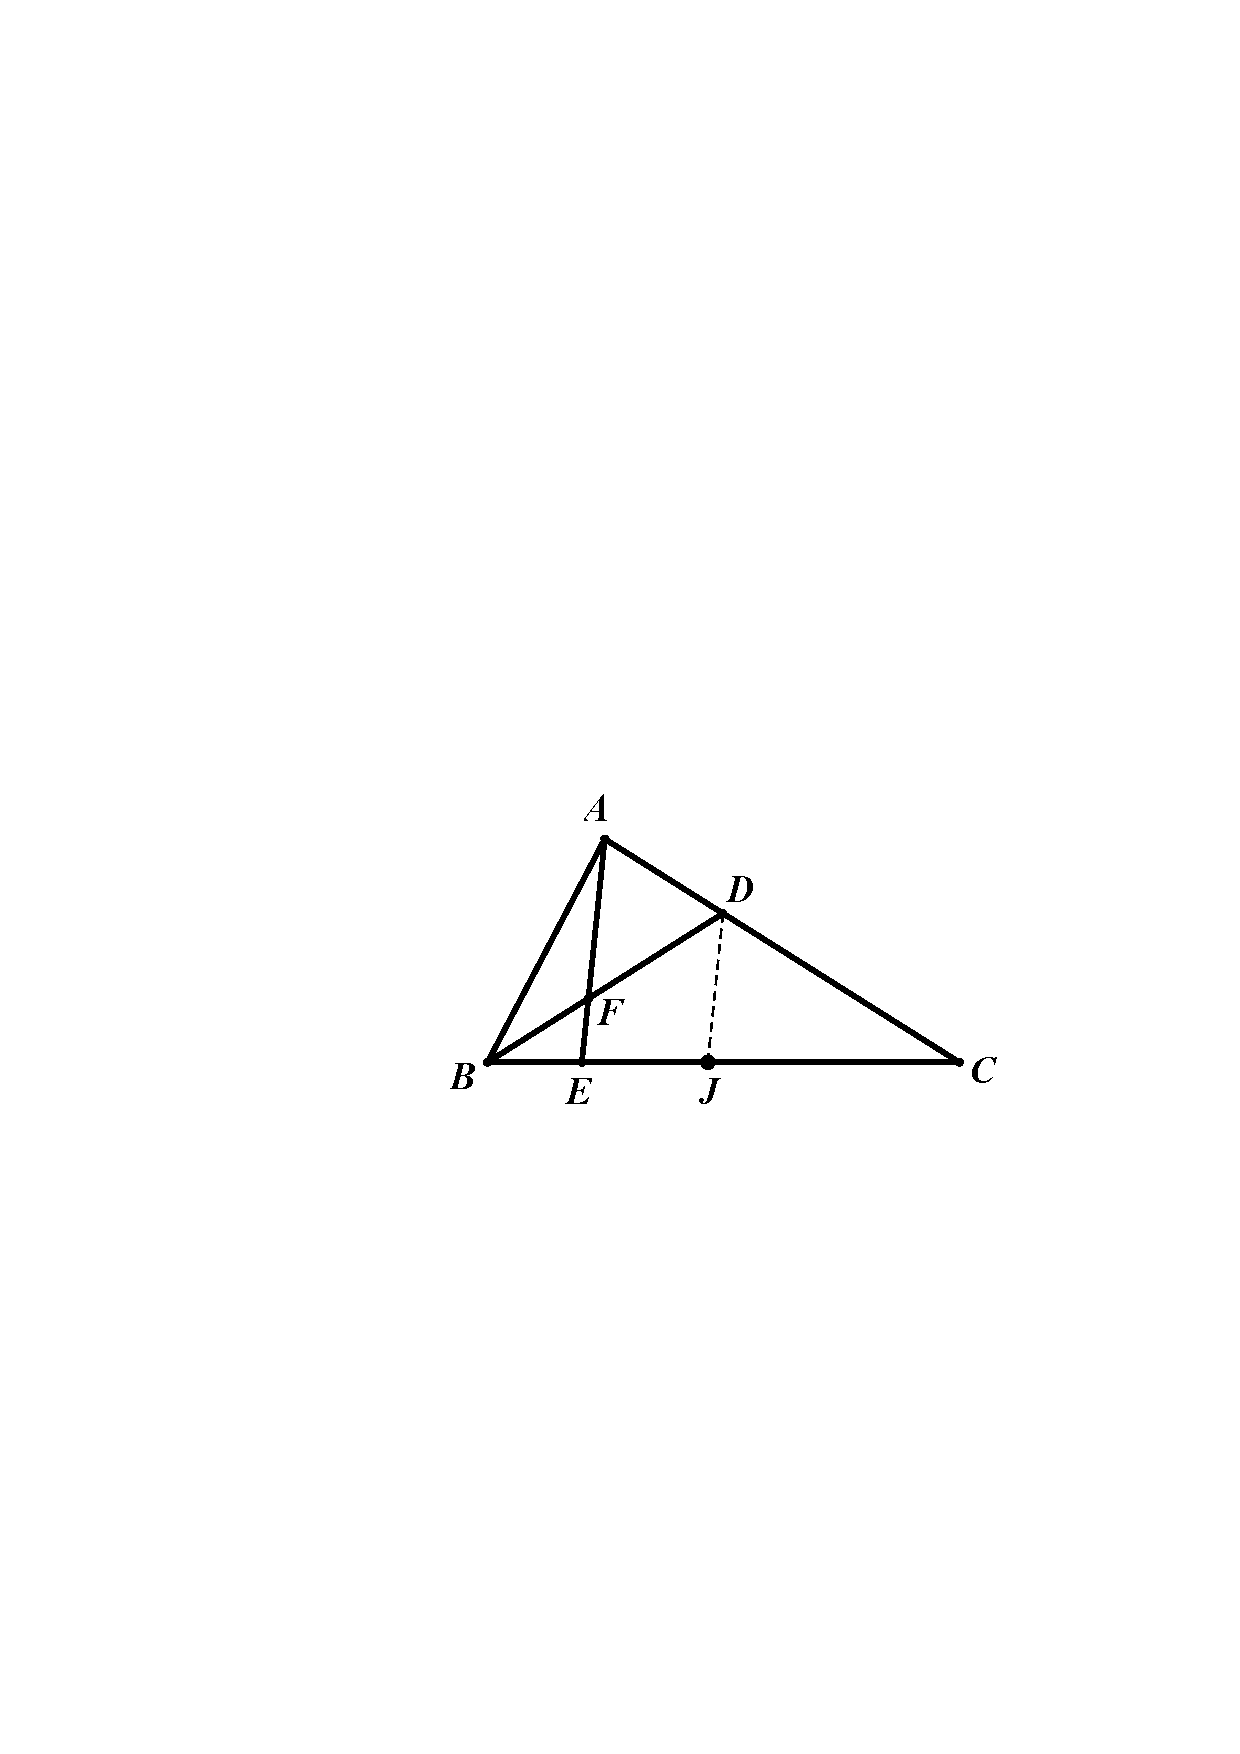
\includegraphics[width=0.3\linewidth]{长度占比习题2-解答}
\end{figure}
$ \dfrac{3}{7} $. 过$ D $作$ AE $的平行线交$ BC $于$ J $点,设$ EJ=x $,则$ EC=3x,\ BE=\dfrac{1}{4}EC=\dfrac{3x}{4},\ BJ=\dfrac{7x}{4},\ \dfrac{BF}{BD}=\dfrac{BE}{EJ}=\dfrac{3}{7} $. 

\item 条件可变形成
\begin{align}\label{垂心条件-变形-习题}
    2\vec{HA}+
    3\vec{HB} +5\vec{HC}=\vec{0}
\end{align}
设 $ \vec{HA}\cdot \vec{HB}=\vec{HA}
\cdot\vec{HC}=\vec{HB}\cdot \vec{HC}=t<0 $,分别用
$ \vec{HB},\vec{HC} $与(\ref{垂心条件-变形-习题})式做数量积,
可得:$ |\vec{HB}|=\sqrt{-\dfrac{7}{3}t} $, $ |\vec{HC}|=\sqrt{-t} $,
$ \cos\angle BHC=\dfrac{\vec{HB}\cdot \vec{HC}}
{|\vec{HB}||\vec{HC}|}=\dfrac{t}{\sqrt{-\frac{7}{3}t}\sqrt{-t}}
=-\dfrac{\sqrt{21}}{7} $,所以$ \cos \angle BAC=\dfrac{\sqrt{21}}{7} $.

\item 
$ \vec{BD}=\mu_1\vec{BC}, \vec{AE} =\mu_2\vec{AD} $,
\begin{align*}
    \vec{AE} =\mu_2\vec{AD} =&\ \mu_2\left[
    (1-\mu_1)\vec{AB}+\mu_1\vec{AC}\right]\\
    =&\ (1-\mu_1)\mu_2\vec{AB}+\mu_1\mu_2\vec{AC} \\
    \vec{AE}=\lambda\vec{AM}+(1-\lambda)
    \vec{AN}=&\ \lambda x\vec{AB}+(1-\lambda)y
    \vec{AC}
\end{align*}
$ \begin{cases}
    \lambda x = (1-\mu_1)\mu_2 \\
    (1-\lambda)y = \mu_1\mu_2
\end{cases} $. 所以$ \dfrac{(1-\mu_1)\mu_2}{x}+\dfrac{\mu_1\mu_2}{y}
=\lambda+1-\lambda=1 $.  \quad $ \dfrac{8}{x}+\dfrac{2}{y}=15 $. \\
(2) $ xy=\dfrac{1}{225}\cdot xy \left(\dfrac{8}{x}+\dfrac{2}{y}\right)^2=
\dfrac{1}{225}\left(\dfrac{64y}{x}+32+\dfrac{4x}{y}\right)\geq\dfrac{64}{225} $. 

\item 在$ \Delta ABC $中,设$ \angle B<\angle C $,
设$ \angle B $的角平分线段长度为$ l_B $,
$ \angle C $的角平分线段长度为$ l_C $,则
\begin{gather*}
    l_B^2=a^2+\left(\frac{1}{2}b\right)^2-2a\cdot \frac{1}{2}b
    \cos C \\
    l_C^2=a^2+\left(\frac{1}{2}c\right)^2-2a\cdot \frac{1}{2}c
    \cos B 
\end{gather*}
两式相减,再使用正弦定理,$ R $代表外接圆半径,
\begin{align*}
    l_B^2-l_C^2= &\ a(c\cos B-b\cos C) +\frac{1}{4}(b^2-c^2) \\
    =&\ R^2[4\sin A(\sin C\cos B-\sin B\cos C)+(\sin^2B-
    \sin^2C)] \\
    =&\ R^2[4\sin(B+C)(\sin C\cos B-\sin B\cos C)+(\sin^2B-
    \sin^2C)] \\
    =&\ R^2[4(\sin B\cos C+\cos B\sin C)(\sin C\cos B-
    \sin B\cos C)+(\sin^2B-\sin^2C)] \\
    =&\ R^2[4(\sin^2C\cos^2B-\sin^2B\cos^2C)+(\sin^2B-
    \sin^2C)] \\
    =&\ R^2\{4[\sin^2C(1-\sin^2B)-\sin^2B(1-\sin^2C)]+(\sin^2B-
    \sin^2C)\} \\
    =&\ 3R^2(\sin^2C-\sin^2B) >0
\end{align*}

\end{enumerate}
\myfootnote{\CopyrightStatementChap}
% {\footnotesize (可在以下空白区域自行增补知识点。)}  
\cleardoublepage

%~\newpage
%~\newpage

%------------------------------------------


